\documentclass[a4paper,titlepage,halfparskip,12pt]{scrreprt}
\usepackage[ngerman]{babel, varioref}
\usepackage[utf8]{inputenc}
\usepackage[T1]{fontenc}
\usepackage{graphicx}
\usepackage{fancyhdr}
\usepackage{amsmath}
\usepackage{geometry}
\geometry{a4paper, top=25mm,left=25mm,right=25mm,bottom=25mm, footskip=12mm}
\usepackage{longtable}
\usepackage{setspace}
\usepackage{lmodern}
%blocksatz
\sloppy
%formatierung literaturverzeichnisangabe
\bibliographystyle{unsrt}

%Auflistungen von Punkten
\usepackage{paralist} 
%urls anzeigen
\usepackage{url}

%farbe
\usepackage{color}															
\usepackage{colortbl}

%landscape
\usepackage{afterpage}
\usepackage{adjustbox}

\usepackage{notoccite}

%Codelisting
\usepackage{xcolor}
\definecolor{mygreen}{rgb}{0,0.6,0}
\definecolor{mygray}{rgb}{0.5,0.5,0.5}
\definecolor{mymauve}{rgb}{0.58,0,0.82}
\definecolor{burntorange}{rgb}{0.8, 0.33, 0.0}
\definecolor{cornellred}{rgb}{0.7, 0.11, 0.11}

% print escaped characters e.g. \n
\newcommand*{\escape}[1]{\texttt{\textbackslash#1}}

\usepackage{listingsutf8}
\lstset{
commentstyle=\color{mygreen},
numberstyle=\small\color{black},
stringstyle=\color{mymauve},
emph={square}, 
showstringspaces=false,
flexiblecolumns=false,
tabsize=2,
numbers=left,
numberblanklines=false,
stepnumber=1,
captionpos=b,
numbersep=5pt,
xleftmargin=15pt,
breaklines=true,
inputencoding=utf8,
extendedchars=true,
extendedchars=true,
basicstyle=\ttfamily\footnotesize,
keywordstyle = \bfseries\color{burntorange},
keywordstyle = [2]\bfseries\color{cornellred},
literate=%
    {Ä}{{\"A}}1%
    {Ö}{{\"O}}1%
    {Ü}{{\"U}}1%
    {ä}{{\"a}}1%
    {ö}{{\"o}}1%
    {ü}{{\"u}}1%
    {ß}{{\ss}}1,%
frame=None,
%frameround=ffff
}

%define Javascript language
\lstdefinelanguage{JavaScript}{
	keywords={typeof, new, true, false, catch, function, return, null, catch, switch, var, if, in, while, do, else, case, break},
	keywordstyle=\color{blue}\bfseries,
	ndkeywords={class, export, boolean, throw, implements, import, this},
	ndkeywordstyle=\color{darkgray}\bfseries,
	identifierstyle=\color{black},
	sensitive=false,
	comment=[l]{//},
	morecomment=[s]{/*}{*/},
	commentstyle=\color{purple}\ttfamily,
	stringstyle=\color{red}\ttfamily,
	morestring=[b]',
	morestring=[b]"
}

%% start defining yaml listings layout
\newcommand\YAMLcolonstyle{\color{red}\mdseries}
\newcommand\YAMLkeystyle{\color{black}\bfseries}
\newcommand\YAMLvaluestyle{\color{blue}\mdseries}

\makeatletter

% here is a macro expanding to the name of the language
% (handy if you decide to change it further down the road)
\newcommand\language@yaml{yaml}

\expandafter\expandafter\expandafter\lstdefinelanguage
\expandafter{\language@yaml}
{
  keywords={true,false,null,y,n},
  keywordstyle=\color{blue}\bfseries,
  basicstyle=\YAMLkeystyle,                                 % assuming a key comes first
  sensitive=false,
  comment=[l]{\#},
  morecomment=[s]{/*}{*/},
  commentstyle=\color{mygreen}\ttfamily,
  stringstyle=\YAMLvaluestyle\ttfamily,
  moredelim=[l][\color{orange}]{\&},
  moredelim=[l][\color{magenta}]{*},
  moredelim=**[il][\YAMLcolonstyle{:}\YAMLvaluestyle]{:},   % switch to value style at :
  morestring=[b]',
  morestring=[b]",
  literate =    {---}{{\ProcessThreeDashes}}3
                {>}{{\textcolor{red}\textgreater}}1     
                {|}{{\textcolor{red}\textbar}}1 
                {\ -\ }{{\mdseries\ -\ }}3,
}

% switch to key style at EOL
\lst@AddToHook{EveryLine}{\ifx\lst@language\language@yaml\YAMLkeystyle\fi}
\makeatother

\newcommand\ProcessThreeDashes{\llap{\color{cyan}\mdseries-{-}-}}

% end defining yaml listings layout

%meta data
\usepackage[hidelinks]{hyperref}
\urlstyle{same}

%akronymverzeichnis
\usepackage[printonlyused]{acronym}

% titel definieren
\newcommand{\titel}{\line(1,0){410}\\ \bigskip Entwicklung eines Instant-Messaging-Systems mit Python\\\bigskip \line(1,0){410}}

%autor definieren
\newcommand{\autor}{Lukas Priester,Oliver Klapper}
\newcommand{\keywords}{\autor,\titel,Studienarbeit}

% Allgemeines für das PDF
\hypersetup{
    pdftitle={\titel},
    pdfauthor={\autor},
    pdfcreator={\autor},
    pdfsubject={\titel},
    pdflang={Deutsch},
    pdfdisplaydoctitle=true,
    pdfkeywords={\keywords},
}

% set distances of chapter headlines in document
\renewcommand*\chapterheadstartvskip{\vspace*{20pt}} % set distance to header
% set distance to text
%\renewcommand*\chapterheadendvskip{%
%  \vspace*{1\baselineskip plus .1\baselineskip minus .167\baselineskip}}

%TODO überall eigene Darstellung unter Abbildungen hinzufügen

\begin{document}

\begin{table}[h]
\centering
\begin{tabular}{lcr}

\includegraphics[height=3.5cm]{images/dhbw-logo}
\end{tabular}
\end{table}
\bigskip
\bigskip
\begin{center}
\vspace*{12mm} {\LARGE\textbf{\titel}}\\
\vspace*{12mm} {\large\textbf{Studienarbeit}}\\
\vspace*{3mm} {\large\textbf{5. - 6. Semester}}\\
\vspace*{12mm} des Studiengangs Informationstechnik (B.Sc.)\\ an der Dualen Hochschule Baden-Württemberg Stuttgart\\
% \vspace*{3mm} an der Dualen Hochschule Baden-Württemberg\\
\vspace*{12mm} von\\
\vspace*{3mm} {\large\textbf{Lukas Priester, Oliver Klapper}}\\
\vspace*{12mm} \today\\
\end{center}
\vfill
\begin{spacing}{1.5}
\begin{tabbing}
mmmmmmmmmmmmmmmmmmmmmmmmmm \= \kill
\textbf{Bearbeitungszeitraum} \> 01.10.2019 - 08.06.2020\\
\textbf{Name, Martrikelnummer, Kurs} \> Oliver Klapper, 7288057, TINF17IN \\
\textbf{Name, Martrikelnummer, Kurs} \> Lukas Priester, 4191693, TINF17IN \\
\textbf{Betreuer der Hochschule} \> Alfred Becker\\
\end{tabbing}
\end{spacing}
%Seitennummerierung ausschalten
\pagenumbering{gobble}
\newpage

\section*{Selbstständigkeitserklärung}

\bigskip

Wir erklären hiermit ehrenwörtlich:

\bigskip

\begin{itemize}
\item[1.] dass wir unsere Studienarbeit mit dem Thema \texttt{Entwicklung eines Instant-Messaging-Systems mit Python} ohne fremde Hilfe angefertigt haben.
\item[2.] dass die Übernahme wörtlicher Zitate aus der Literatur, sowie die Verwendung von Gedanken anderer Autoren an den entsprechenden Stellen innerhalb der Arbeit gekennzeichnet sind.
\item[3.] dass diese Studienarbeit bei keiner anderen Prüfung eingereicht wurde.
\end{itemize}

Wir sind uns bewusst, dass eine falsche Erklärung rechtliche Folgen haben kann.

\bigskip

\begin{small}

\bigskip

\noindent\begin{tabular}{ll}
\makebox[2.5in]{\hrulefill} & \makebox[2.5in]{\hrulefill}\\
Ort, Datum & Lukas Priester \\
\\
\\
\makebox[2.5in]{\hrulefill} & \makebox[2.5in]{\hrulefill}\\
Ort, Datum & Oliver Klapper
\end{tabular}
\end{small}

\newpage

%abstract text
\section*{Abstract}
Communication is an essential part of human existence. A communication can take place in different ways. Due to an increased consumption of electrical devices, communication via digital channels is becoming increasingly important these days. The student thesis includes the implementation of an instant messaging system and is therefore concerned with digital communication.

The goal of the thesis is the design of a functional prototype based on the programming language Python. The understanding of elements of the chat system are summarized in the theoretical basics. As part of the development, two platforms are tested for use in the messaging system. These are the XMPP server ejabberd and the Apache software Kafka. The installation as well as the configuration and integration into the chat system are part of this work. It is up to the user to choose a platform.

The prototype is supported by a user interface that makes the functionalities available to the user in a simpler way. A discussion about the user interface provides information about a suitable module.

With the elaboration of data protection aspects a data protection-friendly implementation is aimed at. For this reason, the development is always based on the data protection guidelines. Defined minimum requirements for the prototype are sufficient for this.

The prototype represents the result of the student research project. It can be assigned functions such as sending and receiving messages. Elements like a REST API, the user interface and an underlying database are also part of the prototype.

The prototype enables communication between users via digital channels.


\newpage

%inhaltsverzeichnis
	% Inhaltsverzeichnis
	\cleardoublepage
	\begin{spacing}{1.1}
		\begingroup
		
			% auskommentieren für Seitenzahlen unter Inhaltsverzeichnis
			\renewcommand*{\chapterpagestyle}{empty}
			\pagestyle{empty}
			
			
			%\setcounter{tocdepth}{1}
			%für die Anzeige von Unterkapiteln im Inhaltsverzeichnis
			\setcounter{tocdepth}{2}
			
			\tableofcontents
			\clearpage
		\endgroup
	\end{spacing}

%% new header/footer settings
\renewcommand{\sectionmark}[1]{\markright{\thesection\ #1}} % make header rightmark
\fancypagestyle{fancyheadlines}{
\pagenumbering{arabic}
\fancyhf{}
\lhead{\slshape\rightmark}
%%\rhead{\slshape\nouppercase{\leftmark}}
\renewcommand{\headrulewidth}{0.4pt}
%\lfoot{\slshape DHBW Stuttgart | Lukas Priester, Oliver Klapper}
\cfoot{\thepage}
\renewcommand{\footrulewidth}{0.4pt}
}

% Redefine the plain page style, show only page number in figure,table,...contents
% and chapter pages
\fancypagestyle{plain}{%
  \fancyhf{}%
  %\lfoot{\slshape DHBW Stuttgart | Lukas Priester, Oliver Klapper}%
  \cfoot{\thepage}
  \renewcommand{\headrulewidth}{0pt}% Line at the header invisible
  \renewcommand{\footrulewidth}{0.4pt}% Line at the footer visible
}


\newpage
\pagenumbering{Roman}

%authorenverzeichnis
\addcontentsline{toc}{chapter}{Autorenübersicht}
\chapter*{Autorenübersicht}
\renewcommand{\arraystretch}{1.5}
\begin{table}[h]
	\centering
	\begin{tabular*}{\linewidth}{lll@{\extracolsep{\fill}}}
		\textbf{Kapitelnr.} & \textbf{Kapitel} & \textbf{Autor} \\
		\hline
		1 & Bedeutung von Instant-Messaging Systemen & Oliver K. \\
		2 & Datenschutzrechtliche Aspekte & Lukas P.\\
		3 & Anforderungen & Oliver K. \\
		4 & Theoretische Grundlagen & Lukas P. \\
		5 & Diskussion über die Art der Benutzeroberfläche & Lukas P.\\
		6 & Verprobung eines Einsatzes von Kafka und &\\
		&Ejabberd in einem Messaging System & Oliver K.\\
		7 & Aufbau und Entwurf der Architektur des Chatsystems & Oliver K.\\
		8 & Ejabberd als moderner Chatserver & Oliver K.\\
		9 & Apache Kafka für moderne Echtzeitübertragung & Oliver K.\\
		10 & Einführung in Python Module für ejabberd und &\\
		& Apache Kafka & Oliver K.\\
		11 & Umsetzung der Entwicklung einer REST API & Oliver K.\\
		12 & Entwicklung der Frontends für den XMPP-Client & Lukas P.\\
		13 & Entwicklung der Frontends für den Kafka-Client & Lukas P.\\
		14 & Gegenüberstellung der Instant Messaging Systeme & Lukas P.\\
		15 & Grundlagen von Softwaretest & Oliver K.\\
		16 & Ergebnis & Oliver K.\\
		17 & Fazit & Lukas P.\\
	\end{tabular*}
	\label{tab:autorenuebersicht}
\end{table}

\pagebreak


%abkürzungsverzeichnis
\cleardoublepage
\addcontentsline{toc}{chapter}{Abkürzungsverzeichnis}
\chapter*{Abkürzungsverzeichnis}
\begin{acronym}[YTMMM]
\setlength{\itemsep}{-\parsep}

\acro{IMS} {Instant Messaging System}
\acro{XMPP} {Extensible Messaging and Presence Protocol}
\acro{XML} {Extensible Markup Language}
\acro{TCP} {Transmission Control Protocol}
\acro{TLS} {Transport Layer Security}
\acro{MUC} {Multi-User-Chat}
\acro{MUC} {Multi User Chat}
\acro{ICQ} {I seek you}
\acro{VoIP} {Voice over IP}
\acro{HTML}{HyperText Markup Language}
\acro{DBMS}{Datenbankenmanagementsystem}
\acro{SQL}{Structured Query Language}
\acro{GUI}{graphical user interface}
\acro{WSGI}{Web Server Gateway Interface}
\acro{CSS}{Cascading Style Sheets}
\acro{Ajax}{Asynchronous JavaScript and XML}
\acro{ORM}{Object Relational Mapper}
\acro{RMI}{Remote Method Invocation}
\acro{RPC}{Remote Procedure Call}
\acro{ASF}{Apache Software Foundation}
\acro{MQ}{Message Queue}
\acro{CA}{Certification Authority}
\acro{RSA}{Rivest-Shamir-Adleman}
\acro{BSI}{Bundesamt für Sicherheit in der Informationstechnik}
\acro{PFS}{Perfect Forward Secrecy}
\acro{ACL}{Access Control List}
\acro{YAML}{YAML Ain't Markup Language}
\acro{DNS}{Domain Name System}
\acro{AES}{Advanced Encryption Standard}
\acro{DES}{Data Encryption Standard}
\acro{SSL}{Secure Socket Layer}
\acro{DOS}{Denial of Service}
\acro{URI}{Uniform Resource Identifier}
\acro{SASL}{Simple Authentication and Security Layer}
\acro{RFC}{Request for Comments}
\acro{MD5}{Message Digest Algorithm 5}
\acro{MAM}{Message Archive Management}
\acro{HTTP}{Hypertext Transfer Protocol}
\acro{REST}{Representational State Transfer}
\acro{API}{Application Programming Interface}
\acro{SSH}{Secure Shell}
\acro{UML}{Unified Modeling Language}
\acro{SSE}{Server-Sent-Events}
\acro{RAM}{Random-Access Memory}
\acro{MIME}{Multipurpose Internet Mail Extensions}
\acro{HTML}{Hypertext Markup Language}
\acro{PDF}{Portable Document Format}
\acro{JSON}{JavaScript Object Notation}
\acro{XML}{Extensible Markup Language}
\acro{JS}{JavaScript}
\acro{DOM}{document object model}
\end{acronym}

%abbildungsverzeichnis
\cleardoublepage
\addcontentsline{toc}{chapter}{\listfigurename}
\listoffigures
\newpage
%tabellenverzeichnis
\cleardoublepage
\addcontentsline{toc}{chapter}{\listtablename}
\listoftables
\newpage
%listingverzeichnis
\cleardoublepage
\addcontentsline{toc}{chapter}{\lstlistingname}
\lstlistoflistings
\newpage

\begin{onehalfspacing}

%% header and footer settings
\pagestyle{fancyheadlines}

\chapter{Bedeutung von Instant-Messaging-Systemen}
\label{chap:Einleitung}

Social Media (deutsche Übersetzung: \glqq soziale Medien\grqq{}) ist ein aktuelles und wichtiges gesellschaftliches Thema. Die vielfältigen und breitgefächerten Nutzungsmöglichkeiten beeinflussen das Privat- und das Berufsleben \cite{gabriel2017social}. Gabriel und Röhrs definieren Social Media in \cite{gabriel2017social} als die Verwendung digitaler Medien unter Einsatz computergeschützter Technologien, das heißt, von Hardware- und Softwaresystemen. Sie definieren den Nutzen von Social Media darin, dass Menschen Informationen suchen, erstellen, verteilen und austauschen können. Es gibt eine große Anzahl an unterschiedlichen Definitionen von Social Media. Nach Liu Yinyuan ist Social Media längst wichtiger Bestandteil des Unternehmensmarketings in Deutschland. In seinem Werk \glqq Social Media in China\grqq{} \cite{liu2016social} beschreibt er, dass in Unternehmen nicht mehr über die grundsätzliche Frage debattiert wird, ob Social Media für das Unternehmensmarketing eingesetzt werden soll, sondern wo und wie Social Media zielgerichtet eingesetzt werden kann. Heutige Unternehmen sind gekennzeichnet von computergestützten Anwendungssystemen, die in allen Funktionsbereichen zur Planung, Steuerung und Kontrolle der Geschäftsprozesse und zu ihrer Verwaltung eingesetzt werden. Sie setzen dieses System in der B2B-Kommunikation (Business-To-Business-Kommunikation) ein. Immer wichtiger werden \ac{IMS}, wie zum Beispiel Whatsapp, Telegram, iMessage und Jabber, die dazu dienen intern Informationen schnell im Unternehmen zu verbreiten, hoch verfügbar zu machen und um Geschäftsprozesse standortunabhängig steuern zu können \cite{gabriel2017social}. Zusätzlich werden Instant Messaging Systeme auch zur externen Kommunikation benutzt. Nach Gabriel und Röhrs ist es möglich, dass mehrere Unternehmen mit Hilfe von innovativen Kommunikationstechniken zur Erreichung eines gemeinsamen Ziels besser kooperieren können. Außerdem ist die schnelle und direkte Kontaktaufnahme von Kunden über ein Messaging System zum Support eines Unternehmens eine einfache und schnelle Möglichkeit, Fragen zum Produkt ohne langes Warten in der Hotline zu stellen. Nach \cite{b2bmehner} werden Nachrichten von Instant-Messaging-Systemen im Gegensatz zu einer E-Mail in Echtzeit übertragen und dem Empfänger direkt zugestellt. Laut einer Statistik von statista benutzen 1,5 Milliarden Nutzer in Deutschland WhatsApp pro Monat \cite{statistaIMS}. Der Anteil der Nutzer von Whatsapp in Deutschland beträgt 75 Prozent an der Gesamtbevölkerung \cite{statistaIMS}. Aus der Statistik  lässt sich folgern, dass Instant-Messaging-Systeme eine Möglichkeit darstellen, Kunden direkter anzusprechen oder Support zu gewährleisten. Eine wichtige Herausforderung von Instant-Messaging-Systemen ist die Einhaltung des Datenschutzes.

\section{Aufgabenstellung}
\label{sec:Aufgabenstellung}

In dieser Arbeit soll gezeigt werden, dass ein Instant-Messaging-System mit der Programmiersprache Python umgesetzt werden kann. Dabei soll diskutiert werden, welche Art von grafischer Oberfläche sich eignet, um dem Benutzer Chatfunktionalitäten bereitzustellen. Die Arbeit beschäftigt sich mit den Echtzeitplattformen Apache Kafka und Ejabberd, welcher das Protokoll \acs{XMPP} verwendet. Die beiden Plattformen sollen benutzt werden, um mit Hilfe von Python ein Chatsystem zu implementieren. Grundlegende Funktionalitäten, wie das Versenden und Empfangen von Nachrichten sollen mit Hilfe von beiden Plattformen und Python implementiert werden. Zusätzlich sollen die beiden Plattformen hinsichtlich ihrer Echtzeitfähigkeit untersucht und verglichen werden. Es soll geprüft werden, ob die Implementierung eines \acs{IMS} mit Apache Kafka in der Programmiersprache Python einfacher ist als über das klassische \acs{XMPP}-Protokoll.

\section{Ziele der Arbeit}
\label{sec:Ziele}

Neben der Umsetzung eines \acs{IMS}, wie in \autoref{sec:Aufgabenstellung} beschreiben, ist das Ziel der Arbeit die Grundlagen eines Instant-Messaging-Systems zu verstehen zu können. Zusätzlich soll über das Protokoll \acs{XMPP} recherchiert werden und dessen Funktionsweise dargestellt werden. Wichtig ist es außerdem, die Funktionsweise und die Grundlagen von den Echtzeitplattformen Ejabberd und Apache Kafka zu verstehen. Die beiden Plattformen sollen mit Hilfe der Programmiersprache Python in das \acs{IMS} integriert werden. Hierfür sind geeignete Python Module durch Recherche zu finden und die Funktionsweise vorzustellen. Ein weiteres wichtiges Ziel ist es, die Umsetzungsschritte und die Lösungen für Problemstellungen, die sich während der Implementierung ergeben, zu beschreiben. Das wichtigste Ziel ist, einen Prototypen des \acs{IMS} zu entwickeln, der grundlegende Chatfunktionalitäten über beide Echtzeitplattformen bereitstellt. Ferner soll durch Recherche und praktischen Entwicklungen das Fachwissen in der Programmiersprache Python vertieft werden. Neben der Recherche von technischen Aspekten, soll sich auch mit den datenschutzrechtlichen Grundlagen von Instant-Messaging-Systemen auseinander gesetzt und beschrieben werden. Das \acs{IMS} soll sich gemäß der Richtlinien des Datenschutzes verhalten.

\pagebreak

\section{Stand der Technik}
\label{sec:StandDerTechnik}

Instant-Messaging-Systeme existieren in der heutigen Form seit Ende der 1990er Jahre, ausgehend von einer Öffnung des Internets für einen größeren Nutzerkreis außerhalb von Forschungsinstitutionen. Das erste \ac{IMS} ist \ac{ICQ} der Firma Mirabilis, welches Benutzern ermöglicht, in einer grafischen Oberfläche Nachrichten untereinander oder in Chatrooms auszutauschen \cite{ICQ}. Die Systeme werden in unterschiedlichen Ausprägungen stets weiterentwickelt. Es kommen zur grundlegenden Funktion des Nachrichtenaustauschs weitere Features, wie Dateiübertragung, \ac{VoIP}, Video over IP, Ende-zu-Ende-Verschlüsselung oder Sprachnachrichten hinzu \cite{gross2007}. 
Weitere typische Funktionen sind die Möglichkeit des Logins mit Passwort und die Angabe der Verfügbarkeit oder die Übermittlung seines Standorts an andere Benutzer. Die Ansprüche an Funktionalitäten von Chatsystemen und der Echtzeitübertragung wachsen stetig weiter und es ist zu erwarten, dass in den kommenden Jahren der Fortschritt die Echtzeitübertragung und die Funktionalitäten von Instant-Messaging-Systeme verbessern wird. Um einen Beitrag zur Steigerung der Präsenz und der Funktionalitäten zu leisten, soll ein Chatsystem gebaut werden, dass einige ausgewählte Anforderungen an gängige Chatsysteme erfüllt.\cite{anastasiaIMS}

\pagebreak

\chapter{Anforderungen}
\label{Anforderungen}

Dieses Kapitel beschreibt allgemeine Anforderungen an das Projekt und an das zu entwickelnde \acs{IMS}. Das Verständnis und die Vollständigkeit aller Anforderungen sind notwendig, um die Studienarbeit erfolgreich umsetzen zu können.

Wichtig ist das Verständnis der Funktionsweise von Instant-Messaging-Systemen und der Plattformen ejabberd und Apache Kafka. Beide Technologien sollen in das \acs{IMS} integriert werden und die Verwaltung von Nachrichten realisieren. Deshalb ist eine umfassende Recherche und Einführung in die beiden Plattformen notwendig und in der Studienarbeit darzustellen. Dabei sind beide Technologien so zu implementieren, dass sie auch ohne das selbst entwickelte \acs{IMS} vollständig benutzt werden können. Das schließt die Verschlüsselung von Daten ein. Wird eine Verschlüsselung verwendet, muss diese aktuell sein und den Empfehlungen von Behörden entsprechen.

Zusätzlich sind Aspekte des Datenschutzes zu berücksichtigen. Diese sollen im Vorfeld durch eine Recherche in Erfahrung gebracht und aufgezeigt werden. Die Konfigurationen sollen den Richtlinien des Datenschutzes entsprechen.

Die Anwendungslogik des \acs{IMS} und die Interaktion mit der jeweiligen Plattform sollen mit einer in Python programmierten Software umgesetzt werden. Dabei ist zu recherchieren und zu diskutieren, welche Art von grafischer Oberfläche geeignet ist, um Benutzern die Funktionalitäten des \acs{IMS} bereitzustellen.

\subsubsection*{Minimale Anforderungen an die Chatfunktionalitäten:}

\begin{itemize}
\item Senden von Nachrichten an Benutzern einer Kontaktliste
\item Empfangen von Nachrichten von anderen Benutzern
\item Nachrichtenarchivierung
\item Benutzer als Kontakt hinzufügen
\item Benutzer des \acs{IMS} müssen sich für alle Aktionen am System anmelden.
\item Ein Benutzer muss sich am \acs{IMS} registrieren können.
\end{itemize}

Die Chatfunktionalitäten aus der oben genannten Auflistung müssen für beide Plattformen, ejabberd und Apache Kafka im \acs{IMS} implementiert werden.

Eine letzte Anforderung ist, die Umsetzbarkeit und die Performanz der beiden Plattformen ejabberd und Apache Kafka zu analysieren. Die Ergebnisse des Vergleichs sind in der Studienarbeit darzustellen und zu begründen.

Als Ergebnis der Umsetzung soll ein Prototyp des \acs{IMS} für eine kleine Anzahl an Benutzern existieren. Gleichzeitige Anmeldungen und Benutzung des Systems sollen aber funktionieren.

Als Unterstützung für die Entwicklung sollen Tests des Programm-Codes der Programmiersprache Python durchgeführt werden. Hierfür soll sich durch eine Recherche mit wichtigen Arten von Fehlern und mit den Möglichkeiten von Software-Tests befasst werden. Wichtige Grundlagen des Testens sind in der Studienarbeit mit Beispielen zu beschreiben.

\pagebreak

\chapter{Datenschutzrechtliche Aspekte}
\label{chap:Datenschutz}
Wird eine Anwendung, ein Webservice oder etwas anderes mehreren Kunden angeboten, kommt schnell das Thema Datenschutz auf. Aus diesem Grund wird der Datenschutz im Rahmen der Studienarbeit erläutert. Mit einem Instant Messaging System werden Kundendaten benötigt. Hinsichtlich der Menge an möglichen Inhalten, werden Kernfragen erarbeitet, welche den Abschnitt in seinem Umfang einschränkt. Dadurch wird das Thema zwar behandelt, aber nicht als Kernaufgabe der Studienarbeit beachtet.\\
Bei den Fragen, welche der Abschnitt umfasst, handelt es sich um die Folgenden:
\begin{itemize}
	\item Wie ist der Datenschutz bei Instant-Messaging Systemen zu beachten?
	\item Wie werden die Daten im Rahmen der Studienarbeit behandelt?
\end{itemize}
An dieser Stelle sei, aufgrund der engen Verknüpfung von Datenschutz und Instant-Messaging, auf den \autoref{chap:Einleitung} zu verweisen. Dieser Abschnitt beinhaltet die Bedeutung von Instant-Messaging-Systemen.

Datenschutz kann je nach Ausführung zu einer eigenen Studienarbeit werden. Zumindest wenn alle Punkte eingehalten werden sollen. In dem Zusammenhang gibt es auch unterschiedliche Interpretationen von Autoren, weshalb der Datenschutz immer mehr an Bedeutung gewinnt. Kai Jendrian sieht bspw. die Enthüllung von Edward Snowden als Wendepunkt der Vertraulichkeit von Kommunikationsdienstleistern. Daraus resultiert das Verhalten der Nutzer nach Alternativen und vor allem sichereren Messaging-Systemen zu schauen. \cite{jendrian14SicheresIM}\\
Interessant ist auch die Herangehensweise von R. Petrlic. In seinem ersten Schritt grenzt er Instant Messaging von E-Mail ab und bildet so einen Übergang von etwas altbewährten zu einem System, welche für die ältere Generation als \glqq neu\grqq\ angesehen wird. In dem  Zusammenhang fallen Schlüsselbegriffe, welche für die Systeme eine Rolle spielen. Die Begriffe sind in der \autoref{img:DatenschutzSchutzziele} dargestellt.
\begin{figure}[h]
	\centering
	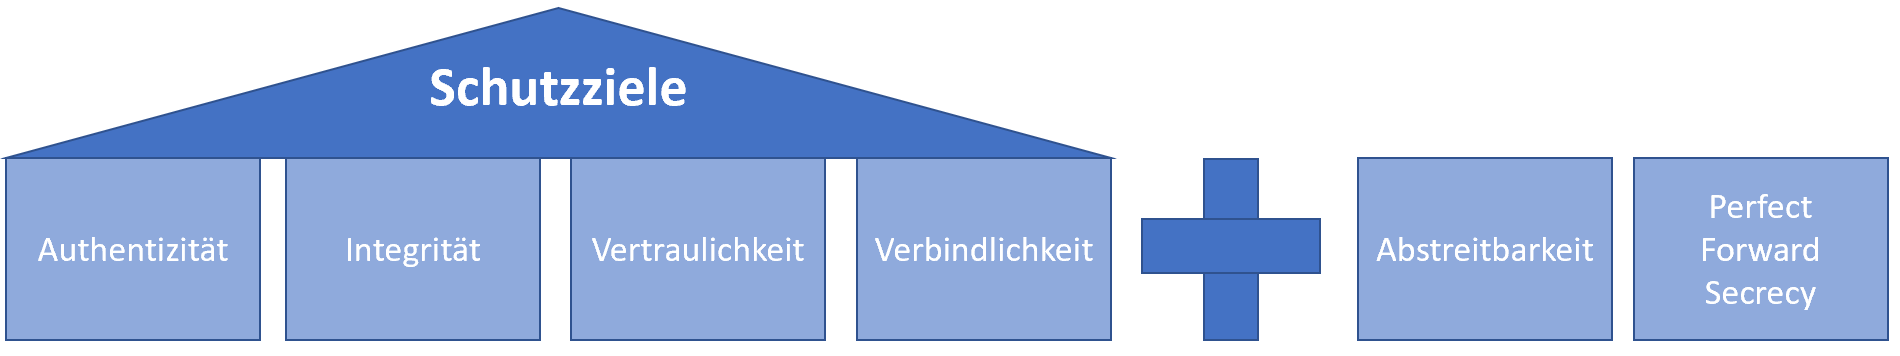
\includegraphics[scale=0.5]{images/DatenschutzSchutzziele}
	\caption{Schutzziele, eigene Darstellung}
	\label{img:DatenschutzSchutzziele}
\end{figure}
Die linken Begriffe aus der Abbildung, werden im Allgemeinen der IT-Security zugeordnet. Petrlic bezeichnet diese als Schutzziele der E-Mail Sicherheit. Durch die private Kommunikation über Instant Messaging-Systeme teilt er auch die rechten Begriffe den Schutzzielen zu. Daher ist bei Instant-Messaging-Systemen auf mehrere Sicherheitsaspekte zu achten. Mit der Abtastbarkeit kommt der Schutz vor einer dritten Partei hinzu. Mit dem Ziel soll gewährleistet werden das die dritte Partei den Urspung der Nachricht nicht verifizieren kann. Mit Perfect Forward Secrecy wird verhindert ältere Nachrichten durch eine Kompromittierung des privaten Schlüssels zu entschlüsseln. Zusätzlich zu den Schutzzielen, fällt im Zusammenhang mit Instant-Messaging-Systemen der Begriff Ende-zu-Ende-Verschlüsselung, welcher gewährleisten soll, dass ausschließlich die Kommunikationspartner die Nachrichten entschlüsseln können. \cite{petrlic2017datenschutz}

Für die Frage nach dem Datenschutz innerhalb der Studienarbeit, bildet sowohl die Thematik als auch die Anforderungen (\autoref{Anforderungen}), den Rahmen wie Daten zu behandeln sind. An dieser Stelle ist auch das allgemeine Recht einer Person zu beachten. Demnach wird der Datenschutz in Deutschland nicht nur durch den Schutz der Daten definiert, sondern durch den Schutz der Person vor Beeinträchtigung in seinem Recht als Persönlichkeit durch Umgang mit seinen personenbezogenen Daten. \cite{petrlic2017datenschutz}\\
In dem Kontext kann das Bundesdatenschutzgesetz zur Rate gezogen werden. Diese beschreiben Datenschutz auch schon bei der Technikgestaltung und den Voreinstellungen. Darin wird explizit aufgeführt so wenig personenbezogene Daten wie nur möglich zu verarbeiten. Das beinhalte sowohl das sammeln an Daten als auch das frühzeitige anonymisieren der Benutzerdaten. Außerdem wird aufgefordert geeignete Maßnahmen zu implementieren, welche diese Anforderungen sicherstellen. Zu der Menge an Daten, lassen sich auch den Umfang an Verarbeitung und die Speicherfristen der Daten hinzuzählen. \cite{bdsg2018}

In Anbetracht der Vielfältigkeit an Anforderungen zur Einhaltung des Datenschutzes ist der Benutzer auf das verarbeiten der Daten hinzuweisen. Mit der Umsetzung eines Messaging-Systems sind verschiedene Schritte notwendig. Ein Schritt beinhalte unter anderem die Implementierung eines datenschutzfreundlichen Systems. Dazu gehört die Berücksichtigung der Anforderungen aus dem oberen Abschnitt. Mit der Definition von Minimalanforderungen an das Chatsystem ist dasselbe für den Datenschutz von Vorteil. Dadurch wird die Kernaufgabe nicht beeinträchtigt. Wobei zu beachten ist, dass ein endgültiger Release alle relevanten Datenschutzverordnungen beinhalten muss. Die minimalen Datenschutzrechtlichen Aspekte gelten lediglich für einen Prototyp des Instant-Messaging Systems. Bei den Minimalanforderungen an Datenschutz handelt es sich um die Folgenden:
\begin{itemize}
	\item So wenig personenbezogene Daten sammeln, wie nur möglich
	\item Größtenteils eine Anonymisierung des Benutzers
	\item Datenschutzhinweise an den Benutzer
\end{itemize}




\pagebreak

\chapter{Theoretische Grundlagen}
\label{chap:Theorie}

Dieses Kapitel beschreibt Grundlagen verschiedener technischer Aspekte, die für die Umsetzung benötigt werden müssen. Ein Verständnis dieser Grundlagen ist wichtig, um ein \acs{IMS} umsetzen zu können.

\section{Funktionsweise von Instant-Messaging-Systemen}
\label{sec:IMSFunktion}

Verschiedene \ac{IMS} besitzen ähnliche Funktionsweisen. Möchte ein Benutzer einen \ac{IMS} nutzen, muss dieser eine bestimmte Software installieren. Diese Software wird als Instant-Messaging-Client (IM-Client bezeichnet. Der Benutzer muss sich an einem Authentifikationsserver registrieren. Es wird ein Benutzerprofil angelegt, welches aus aus einem Benutzernamen (User ID) und einem Passwort (Pre-Shared-Key) besteht. Diese Daten werden beim Login des Benutzers vom \ac{IMS} abgefragt. Ein Benutzerprofil kann weitere personenbezogenen Daten bestehen, wie zum Beispiel, Wohnort, Geschlecht und Geburtsdatum. Die Anzahl der Server für die Authentifizierung und der Bereitstellung des Dienstes variiert je nach der Anforderung an Verfügbarkeit und Anzahl der zu erwartenden Nutzer des \ac{IMS}. Die horizontale Skalierung von Servern und Diensten unterliegt allein dem Betreiber dieser Systeme, häufig finden sich jedoch Cluster-Systeme mit intelligenter Lastverteilung (Load-Balancing). \autoref{img:StrukturIMS} zeigt den allgemeinen Aufbau eines \ac{IMS}.\cite{anastasiaIMS}

\begin{figure}[h]
	\centering
	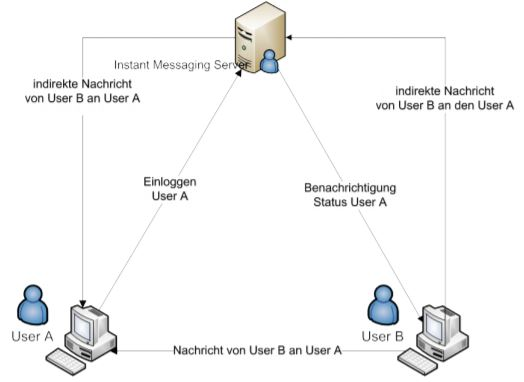
\includegraphics[width=.65\textwidth]{images/GrundlegendeStrukturIMS}
	\caption{Allgemeine Struktur eines Instant-Messaging-Systems \cite{anastasiaIMS}}
	\label{img:StrukturIMS}
\end{figure}

In der Abbildung wird eine horizontale oder vertikale Skalierung des \ac{IMS} vernachlässigt. Der Authentifikationsserver symbolisiert einen oder mehrere Server. Hat sich der Benutzer mit seinen Login-Daten erfolgreich gegenüber dem Authentifikationsserver authentifiziert, kann er andere, bereits registrierte, Benutzer kontaktieren. Die Verbindungsinformationen wie zum Beispiel IP-Adresse, die dem Client lokal zugewiesene Portnummer und die Kontaktliste (Freunde des Benutzers) werden an den Präsenzserver übermittelt. Dieser ist abhängig von der Implementierungsform ein Teil des IM-Servers oder ein eigenständiger Server. Der Präsenzserver überprüft, welche Benutzer aus der Kontaktliste verfügbar und angemeldet sind. Der Server sendet dem Benutzer die Ergebnisse der Statusüberprüfung zurück. Ist einer der gewünschten Benutzer \glqq online\grqq\ (verfügbar) kann durch die Auswahl der entsprechenden Kennung eine Verbindung aufgebaut werden und der Nachrichtenaustausch kann beginnen. Das ist möglich, weil der Server dem Sender die IP-Adresse und die Ziel-Portnummer des Kommunikationspartners übermittelt. Die Nachrichten werden direkt zwischen den Clients übertragen oder über den Server zwischen den Kommunikationspartnern übermittelt. Die Art der Übertragung ist von System zu System je nach Realisierung unterschiedlich. Der Kommunikationspfad ist abhängig von der Architektur und dem verwendeten Protokoll. Eine Nachricht kann zentral über den Server vermittelt werden (siehe \autoref{img:StrukturIMS}-indirekte Nachricht) oder nach dem Peer-to-Peer-Prinzip (siehe \autoref{img:StrukturIMS}-direkte Nachricht).

\section{XMPP-Extensible Messaging and Presence Protocol}
\label{sec:XMPP}
\ac{XMPP} bedeutet Extensible Messaging and Presence Protocol. Wird dieses ins Deutsche übersetzt, so entsteht die Bedeutung eines erweiterbares Nachrichten- und Anwesenheitsprotokoll. Eine Definition die \ac{XMPP} sehr gut beschreibt. \ac{XMPP} basiert auf \ac{XML}, welches eine Markup Sprache darstellt. Das Ziel von \ac{XMPP} war ein Protokoll für das Instant Messaging zu entwickeln. Laut dem RFC6120 lässt sich mittels \ac{XMPP} Daten zwischen zwei oder mehreren Netzwerkeinheiten nahezu in Echtzeit austauschen, welches als Vorteil für Sofortnachrichten bezeichnet werden kann. Diesbezüglich nutzt es das Internet und erlaubt den Usern Sofortnachrichten an andere Anwender innerhalb des Internets zu schicken. \ac{XMPP} lässt sich in viele verschiedene Funktionen aufteilen, weshalb der grundlegende Zweck ein anderes Ziel verfolgt. Im einfachsten Sinne ist die Idee von \ac{XMPP} den Austausch von kleinen Teilen strukturierter Daten (\glqq \ac{XML} stanzas\grqq\ zwischen einem oder mehreren Netzwerkteilnehmern zu ermöglichen. Primär wird \ac{XMPP} mithilfe einer Client-Server-Architektur implementiert, bei der sich ein Client mit einem Server verbindet, um mit anderen Teilnehmern Daten auszutauschen. Anderseits kann es als Protokoll auch zwischen Servern fungieren. Daraus resultiert der Vorteil nahezu unabhängig von Betriebssystemen und Browsern zu sein. Wird die Client-Server-Architektur implementiert, so ist in der Regel der Ablauf definiert durch folgende Schritte: \cite{RFC6120} 
\begin{enumerate}
	\item Bestimmen der IP-Adresse und des Ports zu dem sich verbunden werden soll 
	\item Eine \ac{TCP} Verbindung öffnen/aufbauen
	\item Öffnen eines \ac{XML}-Streams über \ac{TCP}
	\item Optional: Verwendung von \ac{TLS} für die Verschlüsselung
	\item Verwendung des SASLs Frameworks für die Authentifizierung
	\item Eine Ressource an den \ac{XML} stream anbinden
	\item Austausch unbegrenzter \glqq \ac{XML} stanzas\grqq\ ()=> kleine Teile strukturierter Daten) mit anderen Netzwerkteilnehmern
	\item Schließen des \ac{XML} streams
	\item Schließen der \ac{TCP} Verbindung
\end{enumerate}

\pagebreak

Die folgende \autoref{img:XMPPcommunication} zeigt den Start einer Kommunikation, wie im genannten Ablauf dargestellt, über \ac{XMPP} und den \ac{XML}-streams.

\begin{figure}[h]
	\centering
	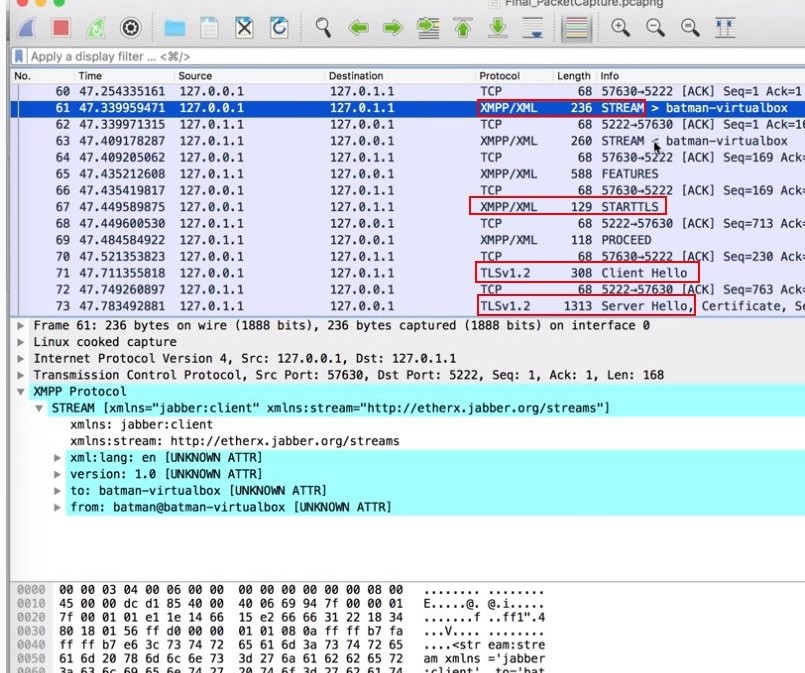
\includegraphics[width=\textwidth]{images/XML_Wireshark}
	\caption{Kommunikationsaufbau des \ac{XMPP}-Protokolls} %TODO Quelle fehlt
	\label{img:XMPPcommunication}
\end{figure} 

Für den Austausch von Daten gibt es zwei elementare Konzepte. Zum einen die \ac{XML}-Streams und die \ac{XML}-Stanzas. Diese zwei Konzepte werden definiert um das Verständnis des Datenaustauschs, wie es im obigen Ablauf definiert ist, zu erlangen. Bei dem Austausch der Daten mittels \ac{XML} streams wird von einem Container zwischen den Teilnehmern gesprochen. Der \ac{XML} stream ist durch den \glqq stream header\grqq\ (z.B. \ac{XML} <stream>) und dem Ende des streams, dargestellt durch \ac{XML} </streams>, eindeutig definiert. Die Anzahl der austauschbaren \ac{XML} Elemente ist unbegrenzt und durch die Lebensdauer des streams definiert. Das \ac{XML} stanza wird nun als diskrete semantische Einheit strukturierter Daten, das von einem Teilnehmer zu einem anderen über den \ac{XML} stream gesendet wird bezeichnet. Das \ac{XML} stanza ist ein direktes Kind-Element des streams. Ein stanza kann wiederum selbst Kind-Elemente enthalten, das den \ac{XML} stream definiert. Im Kern fungiert der \ac{XML} stream wie eine Hülle um alle \ac{XML} stanzas, die während einer Session versendet werden.

\pagebreak

Ein Aufbau kann wie in der folgenden \autoref{img:StrukturXMLstream} repräsentiert werden. \cite{RFC6120Sec4}
\begin{figure}[h]
	\centering
	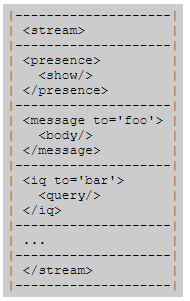
\includegraphics[scale=1.2]{images/XML_Stream}
	\caption{Allgemeine Struktur eines XML streams} %TODO Quelle fehlt
	\label{img:StrukturXMLstream}
\end{figure}

\pagebreak

\section{Grundlagen von Datenbanken}
\label{sec:Datenbank}
Für den Aufbau eines Chatsystems ist ein Datenbanksystem notwendig. Die Datenbank wird benötigt, weil Informationen und Parameter für die Authentifizierung des Benutzers gespeichert werden müssen. Außerdem ist die interne Datenbank Mnesia eines Ejabberd-Chatservers nicht für den Mehrbenutzer-Betrieb ausgelegt. Mnesia ist in der Sprache Erlang entwickelt. Sie besitzt eine weiche Echtzeitfähigkeit und ist auf Geschwindigkeit optimiert \cite{MnesiaDoc}. Die verfügbare Speicherkapazität von maximal 2 Gigabyte für den Betrieb ist nicht ausreichend für ein Mehrbenutzer-System \cite{ejabberdDoc}. Ein Mehrbenutzer-Betrieb eines ejabberd-Servers benötigt eine Datenbank, in der Nachrichtenverläufe, Kontakte jedes Benutzers und weitere Parameter gespeichert werden können.

Eine Datenbank beinhaltet eine Sammlung von mehreren Daten, die sich aufeinander beziehen können, und von einem \ac{DBMS} verwaltet werden. Kernkomponente für den Zugriff ist die einheitliche logische Schnittstelle zum \ac{DBMS}. Auf die Daten und Schnittstellen des \acs{DBMS} können mit der Programmiersprache \ac{SQL} zugegriffen werden. Dafür wird der Datenbank über \ac{SQL} nur mitgeteilt welche Daten benötigt werden. Ein Datenbanksystem muss bestimmte Eigenschaften besitzen, um den Zweck Daten zu speichern und sie wieder abzufragen, zu erfüllen.

\smallskip

\textbf{Eigenschaften:}
\begin{itemize}
	\item Unabhängigkeit von dem physischen Aufbau
	\item Schutz bei (Mehrfach-) zugriff auf Daten
	\item Integrität
	\item Zuverlässigkeit
	\item Ausfallsicherheit
\end{itemize}

Es gibt verschiedene Datenbankmodelle, nach denen eine Datenbankstruktur definiert wird. Die Datenbankmodelle unterteilen sich in relationale, objektorientierte, hierarchische und netzwerkartige sowie in moderne Datenbanken. Für die Projektarbeit wird ein relationales Datenbankmodell verwendet und deshalb dieses Modell genauer vertieft. Dementsprechend sind wichtige Schlüsselbegriffe zu definieren. Eine Tabelle wird ebenfalls als Relation bezeichnet(\autoref{img:RelationDB_Begriffe}). Eine Zeile der Relation heißt Tupel, die Spalten Attribute. Die Kardinalität entspricht der Anzahl von Tupeln und der Grad bezieht sich auf die Anzahl der Attribute. Ein wesentliche Bestandteil einer relationalen Datenbank ist der Primärschlüssel, welcher zwingend erforderlich ist und eindeutig sein muss. Der Schlüsselbegriff Gebiet bezieht sich auf ein Definitionsbereich eines Attributes, welches alle gültigen Werte für dieses Attribut umfasst. \cite{Schicker2017}

\textbf{Beispiel einer Relation:}

\smallskip

\begin{figure}[h]
	\centering
	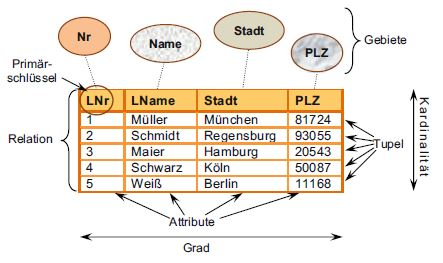
\includegraphics[scale=1.2]{images/RelationMitSchluesselbegriffe}
	\caption{Relation mit Schlüsselbegriffe \cite{Schicker2017}}
	\label{img:RelationDB_Begriffe}
\end{figure}

Eine relationale Datenbank ist definiert als eine Datenbank mit einer Ansammlung von zeitlich variierenden, normalisierten Relationen mit passenden Graden.
MySQL ist eines der weltweit verbreitetsten relationalen Datenbanksysteme, weil sie als Open-Source-Software und als kommerzielle Enterprise-Version verfügbar ist. MySQL wird von allen gängigen Betriebssystemen wie Linux oder Windows unterstützt. Entwickelt wird MySQL von der Oracle Cooperation. Die MySQL-Datenbanken sind relational und orientieren sich an den oben genannten Schlüsselbegriffen, die eine relationale Datenbank definieren. Die MySQL-Datenbank ist in der Software eine Client-Server-Architektur, die aus einem Multi-Threading-Server besteht. Dadurch werden verschiedene Backends, Clientprogramme und Verwaltungswerkzeuge parallel unterstützt.\cite{MysqlDoc}
\newpage

\section{Grafische Benutzeroberfläche}
\label{sec:Benutzeroberfläche}
Eine Grafische Benutzeroberfläche ist im Detail eine Schnittstelle zwischen einem Computer und einem Nutzer. Die im Hintergrund agierende Software soll mittels Symbole und anderen Elementen bedienbar gemacht werden. Im Englischen wird die Benutzeroberfläche als \ac{GUI} bezeichnet, welches im weitere Verlauf ebenfalls als Bezeichnung verwendet wird. Allgemein besitzt eine \ac{GUI} Bedien- und Steuerelement die mit der im Hintergrund laufenden Software interagiert. Der Einsatz einer \ac{GUI} liegt an der Usability, welches die Benutzerfreundlichkeit beschreibt. Eine \ac{GUI} soll demnach dem User die Möglichkeit geben, die Software auch ohne großen Aufwand bedienen zu können. Eine Eigenschaft die heutzutage nahezu jedes Programm beinhalten muss. \cite{thesmann2016interface}

Im Rahmen der GUI-Programmierung müssen mehrere Aspekte berücksichtigt werden um die Usability zu erfüllen. Dafür werden die Aspekte in 8 goldene Regeln zusammengefasst.
\begin{enumerate}
	\item Strebe nach Konsistenz
	\item Sorge für universelle Bedienbarkeit
	\item Biete informative Rückmeldung
	\item Entwerfe abgeschlossene Dialoge
	\item Biete einfache Fehlerbehandlung
	\item Lass die Einfache Umkehrung von Aktionen zu
	\item Vermittle ein Gefühl der Kontrolle
	\item Entlaste das Kurzzeitgedächtnis
\end{enumerate}
Im Folgenden wird kurz auf die 8 Regeln eingegangen.

Der erste Punkt, Strebe nach Konsistenz, befasst sich bspw. mit dem Erscheinungsbild einer Seite. Die Seite sollte dem Aspekt zur Folge die Elemente, wie einen Button, immer an der gleichen Stelle positionieren.

Der nächste Punkt, Sorge für universelle Bedienbarkeit, beinhaltet Anforderungen an Bedienelementen. Somit sollte jeder Nutzer die Bedienung und Kürzel ohne Einschränkungen verstehen können.

Ein Nutzer verlangt nach ausreichendem Feedback, die vor allem informativ und in vielen Fällen auch hilfreich sind. Ein Fakt der im dritten Punkt, Biete informative Rückmeldung, behandelt wird.

Der vierte Gesichtspunkt, Entwerfe abgeschlossene Dialoge, umfasst die Führung eines Nutzers, zum Beispiel durch einen Verkaufsprozess. Zu jedem Zeitpunkt soll der Nutzer wissen, in welchem Prozess er sich befindet.

Um die Bedürfnisse der Nutzer gerecht zu werden, muss wie in Punkt fünf, Biete einfache Fehlerbehandlung, definiert, die Fehler mit nützlichen Informationen für den Nutzer ausgestattet werden. Außerdem muss ein Ausweg in den normalen Programmablauf gewährleistet sein.

Ein Nutzer soll mit Punkt sechs, Lass die Einfache Umkehrung von Aktionen zu, die Möglichkeit haben kleine Ereignisse rückgängig zu machen.

Der siebte Gesichtspunkt, Vermittle ein Gefühl der Kontrolle, beinhaltet die Aktion und Reaktion. Demnach soll die Software auf eine Aktion des Nutzers reagieren und nicht andersrum. 

Der letzte Punkt, Entlaste das Kurzzeitgedächtnis, soll gewährleisten, dass die \ac{GUI} schlicht und einfach gehalten wird. Ein Nutzer sollte sich keine große Anzahl an Informationen merken müssen um einen Aktion auszuführen.
\cite{UI8Regeln2019}

Mit Betrachtung dieser 8 goldenen Regeln kann die grafische Benutzeroberfläche bei der Ausführung erfolgreich umgesetzt werden.


\section{HTML, CSS und JavaScript als Werkzeuge der Webentwicklung}
\label{sec:HTMLCSSJS}
Für ein grafische Benutzeroberfläche im Web werden Elemente benötigt, die das Erscheinungsbild aufbauen, gestalten und mit Dynamik verknüpfen. Dafür werden die Werkezeuge des Webdesign benötigt. Diese umfassen \ac{HTML}, \ac{CSS} und \ac{JS}.

\textbf{\ac{HTML}}\\
Das Internet mit seinen Funktionen Text-, Bild, Sound und weiteres abzubilden oder zu übertragen basiert auf einem gemeinsamen Standard. Dieser ist unter dem Namen Hypertext Markup Language \ac{HTML} bekannt, welcher zu deutsch unter einer Auszeichnungssprache zu verstehen ist. Konkret bezieht sich \ac{HTML} auf Hypertexte die per Definition die Verlinkung zwischen Texte mithilfe von Hyperlinks bezeichnen. \ac{HTML} als Markup Language entstand schon 1989 und diente zur Beschreibung und Verlinkung von Text. Mit \ac{HTML}5, welches ergänzend zur ersten Variante auch Audio- oder Videodateien an die Webseite binden kann, befindet sich die aktuellste Version im Umlauf. Während eine Weboberfläche unabhängig vom Betriebssystem ist, spielt die Verwendung von Browsern, die ihre eigenen HTML-Parser besitzen, eine bedeutsame Rolle. Aus diesem Grund können vom Webserver ausgelieferte \ac{HTML}-Dateien bei einer geringen Anzahl an Browsern Probleme bereiten. Innerhalb eines \ac{HTML}-Dokuments ist vor allem das Grundgerüst und der Aufbau relevant. Demnach werden die Elemente einer Webseite mit Sprachelementen, sogenannten Tags, beschrieben. Der Aufbau eines Grundgerüst ist in der \autoref{img:GrundgeruestHTML} dargestellt.
\begin{figure}[h]
	\centering
	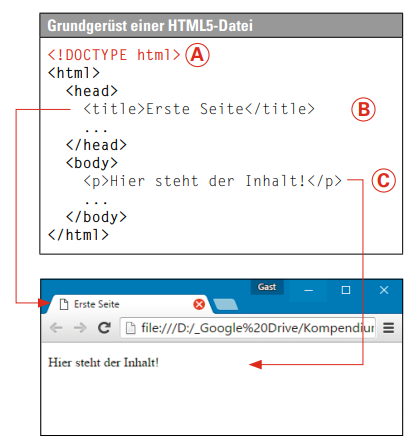
\includegraphics[scale=1.3]{images/HTML_Grundgeruest}
	\caption{Grundgerüst einer HTML-Datei, \cite{buhler2017html5}}
	\label{img:GrundgeruestHTML}
\end{figure}
\\Der \autoref{img:GrundgeruestHTML} sind die 3 wichtigen Tags (html, head, body) eines Standard \ac{HTML}-Dokumentes sowie der unter A angegebenen Dokumenttyp zu entnehmen. Während in vielen Programmiersprachen die Syntax umfassend groß sein kann, ist die Grammatik bei \ac{HTML} schlicht. Für die Korrektheit sind daher die genannten Tags bedeutend. Außerdem werden überwiegend Verschachtelung bei der Darstellung einer Webseite benötigt. Für einen weiteren Einfluss auf die Tags können sogenannte Attribute, wie in der folgenden \autoref{img:HTMLattribute} dargestellt, dem jeweiligen Tag zugeordnet werden. 
\begin{figure}[h]
	\centering
	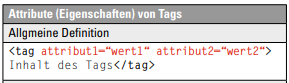
\includegraphics[scale=2.5]{images/HTMLattribute}
	\caption{Attribut eine \ac{HTML}-Tags, \cite{buhler2017html5}}
	\label{img:HTMLattribute}
\end{figure}
\\Als Resultat geht hervor, dass der Kern einer \ac{HTML}-Datei die Tags darstellen. Während nun das Dateiformat als reine Textdatei vorliegt, entstehen Fragen über die gestalterischen Aspekte wie z.B. Farben, Grafiken, Videos oder ähnliches. Hauptsächlich werden diese Aspekte innerhalb einer \ac{CSS}-Datei behandelt, dennoch gibt es dafür Merkmale, die in einer \ac{HTML}-Datei zu beachten sind. Um beispielsweise Grafiken oder Videos, die sich innerhalb eines anderen Unterordners befinden, zu integrieren, muss auf diese referenziert werden. Hierfür bietet \ac{HTML} die absolute und relative Referenz. Eine absolute Referenz, wie z.B. \textit{C:/Dokumente/Mustermann/Eigene Dateien/Webseiten/button.gif}, wird aufgrund der Abhängigkeit zum User des Computers nicht verwendet. Für die relative Referenz ist wiederum eine einheitliche Ordnerstruktur wichtig, da der Pfad von dem Speicherort der \ac{HTML}-Datei angegeben wird. Diese Struktur kann, wie in der folgenden \autoref{img:TreeHTMLStruktur} dargestellt, aussehen.
\begin{figure}[h]
	\centering
	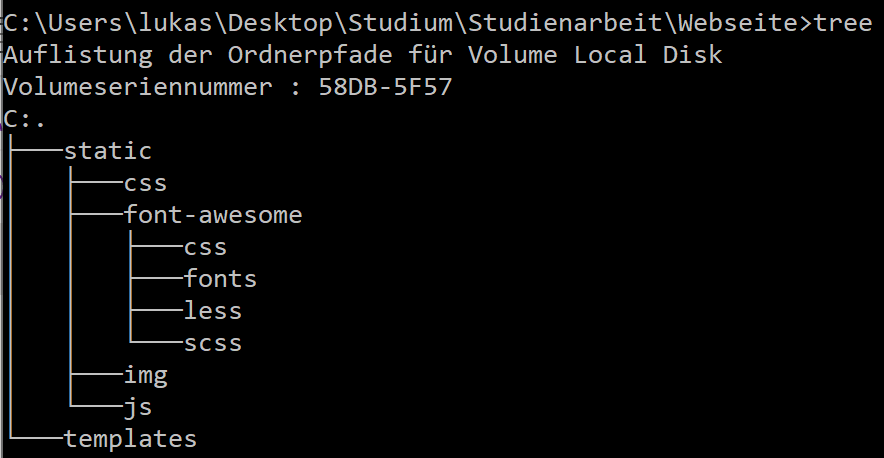
\includegraphics[scale=0.8]{images/TreeHTMLStruktur}
	\caption{Ordnerstruktur bei der Webentwicklung, eigene Darstellung} 
	\label{img:TreeHTMLStruktur}
\end{figure}
\\Demnach würde die \ac{HTML}-Datei in dem Ordner \textit{templates} liegen und die Bilder im Ordner \textit{static/img}, welcher über die relative Referenz unabhängig vom Betriebssystem und ähnliches erreicht werden kann. Je nach Dateityp orientieren sich auch die Tags innerhalb des \ac{HTML}-Dokumentes an den zu implementierenden Medientyp. Für eine Grafik gibt es daher den \texttt{img}-Tag, der die Referenz zum Bild enthält. Mit der Webentwicklung wird das Ziel verfolgt Inhalt und Gestaltung strikt voneinander zu trennen. Daher werden \ac{CSS}-Dateien, die sich mit dem Design befassen, benötigt.\cite{buhler2017html5}

\textbf{CSS:}\\
Die Dateien, die als \ac{CSS} deklariert werden, übernehmen die gestalterischen Aspekte, die ein \ac{HTML}-Dokument nicht erfüllen kann. Neben Designvarianten bietet \ac{CSS} auch die Möglichkeit, die Webseite an das jeweilige Endgerät, unterschiedlicher Auflösung, anzupassen. Wie schon für die \ac{HTML}-Dateien gilt auch für \ac{CSS}, dass Attribute nur von bestimmten Browsern akzeptiert werden. Daher gehört zur Webentwicklung ein ausgiebiges Testen dazu. Eine \ac{CSS}-Datei sollte Regeln folgen um Probleme, die im Zusammenhang mit dem HTML-Dokument auftreten können, zu verhindern. Die Grundregel bezieht sich auf den Ort der \ac{CSS}-Definition. Diese kann zum Einen in einer externen Datei, intern in einem eigenen Tag definiert, oder in ein \ac{HTML}-Tag integriert werden. Das ist unter anderem relevant wenn mehrere \ac{CSS}-Dateien zum Einsatz kommen, weil die verschieden Orte durch verschiedene Prioritäten geprägt sind. Allgemein wird die \ac{CSS}-Definitionen in eine eigene Datei ausgelagert um das Design und die \ac{HTML}-Datei zu trennen. Die \autoref{img:CSSrules} stellt dar, wie eine \ac{CSS}-Definition aufgebaut ist.
\begin{figure}[h]
	\centering
	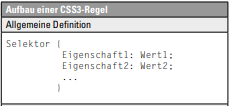
\includegraphics[scale=2.5]{images/CSS_Definition}
	\caption{Aufbau einer \ac{CSS}-Regel, \cite{buhler2017html5}}
	\label{img:CSSrules}
\end{figure}	
\\Der Aufbau besteht grundlegend aus einem Selektor, dem seine Eigenschaften bearbeitet werden sollen. Damit die Auswirkungen erkennbar werden, muss die \ac{CSS}-Datei mit dem HTML-Dokument verknüpft werden. Das geschieht innerhalb des Head-Tags in der \ac{HTML}-Datei, mit Hilfe des \texttt{link}-Tags \texttt{<link rel=\dq sytlesheet\dq \;type=\dq text/css\dq \;href=\dq design.css\dq>}. Der Selektor befindet sich immer vor einer geschweiften Klammer und kann unterschiedlich verwendet werden. Aufgrund der Verbindung zur HTML-Datei hängt der Selektor vom \ac{HTML}-Tag ab. Wird bspw. ein Button in dem \ac{HTML}-Tag als Klasse definiert, so wird über den Punkt zugegriffen. Wird jedoch der Button mit einer ID ausgestattet, so muss mit dem Rautezeichen darauf zugegriffen werden. Die nachfolgende Abbildung zeigt diese Varianten.
\begin{figure}[h]
	\begin{minipage}[c]{.4\textwidth}
		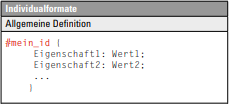
\includegraphics[width=\textwidth]{images/CSSID}
		\caption{Zugriff über ID, \cite{buhler2017html5}} 
		\label{img:CSSID}
	\end{minipage}
	\hspace{.1\linewidth}% Abstand zwischen Bilder
	\begin{minipage}[c]{.4\textwidth}
		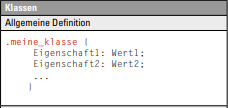
\includegraphics[width=\textwidth]{images/CSSKlasse}
		\caption{Zugriff über Klasse, \cite{buhler2017html5}}
		\label{img:CSSClass}
	\end{minipage}
\end{figure}
Für die Eigenschaften bietet sich mit der dritten Version von \ac{CSS} (\ac{CSS}3) eine Vielzahl an Möglichkeiten. Grundlegend kann jedes Element mithilfe der \ac{CSS}-Datei bearbeitet werden. Die Eigenschaften sind bspw. unter Typografie, Farbe, Abstände, Tabellen und vieles mehr gegliedert. In diesem Zusammenhang ist auch die Verwendungen von Ma"seinheiten bedeutsam. Mit \ac{CSS}3 werden viele verschiedene Ma"seinheiten unterstützt worüber die \autoref{img:CSSmasseinheiten} einen genaueren Überblick gibt.
\begin{figure}[h]
	\centering
	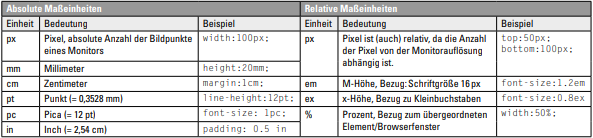
\includegraphics[scale=1.8]{images/CSSmasseinheiten}
	\caption{Ma"seinheiten innerhalb der Webentwicklung, \cite{buhler2017html5}} 
	\label{img:CSSmasseinheiten}
\end{figure}
\ac{CSS} verwendet die Selektoren und wendet auf diesen die definierten Eigenschaften an. Nebenbei bietet \ac{CSS} die Möglichkeit an, ein Layout zu erstellen. Dafür ist das sogenannte Boxmodell ausschlaggebend. Dieser ist definiert, die Elemente als eine Box mit Eigenschaften zu betrachten. Demnach gibt es in dem Zusammenhang vielerlei Möglichkeiten eine Box an die richtige Position, sowie mit der richtigen Größe abzubilden. Die Boxen können mit absoluten Werten definiert werden. Mit relativen Werten, welche Prozentwerte enthalten, können die Boxen sich in Abhängigkeit des Browserfensters ändern. Mit \ac{CSS}3 gibt es ebenso die Möglichkeiten flexible Boxen zu verwenden. Dadurch werden die Boxen unabhängig von der Position und Anordnung spalten- oder zeilenweise an den zur Verfügung gestellten Platz angeordnet. Bei der Betrachtung des Layouts spielt genauso das Endgerät eine Rolle. In dem Zusammenhang können Media Queries zum Einsatz kommen. Diese bieten die Option, Eigenschaften eines Selektors entsprechend der angegebenen Pixel zu ändern.
\begin{figure}[h]
	\centering
	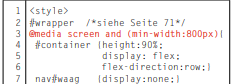
\includegraphics[scale=2.8]{images/MediaQbsp}
	\caption{Beispiel eines Media Queries, \cite{buhler2017html5}}
	\label{img:/MediaQbsp}
\end{figure}
\\Die \autoref{img:/MediaQbsp} stellt dar wie die Media Queries eingesetzt werden können. Diese werden entweder in der \ac{CSS}-Datei oder in dem Style-Tag einer \ac{HTML}-Datei definiert. Mit diesen Grundlagen lassen sich Seiten gestalterisch anpassen und auf mehreren mobilen Endgeräten ausgeben. Werden Inhalte benutzt, die sich ggf. zur Laufzeit ändern, wird überwiegend auf das dritte Element der Webentwicklung zurückgegriffen. Hierbei handelt es sich um JavaScript.\cite{buhler2017html5}

\textbf{JavaScript}\\
JavaScript verfolgt das Ziel interaktive oder dynamische Elemente auf der Webseite zu integrieren. Es ist eine Skriptsprache, die überwiegend auf Seiten des Clients eingesetzt wird. Der Code kann direkt über den Browser ausgeführt werden, da ein heutiger Browser einen Interpreter für die Skriptsprache besitzt. Dadurch ist JavaScript von den heutigen Browsern abhängig, weshalb das Web Frontend auf verschiedenen Browsern getestet werden muss. Mit JavaScript ergeben sich Möglichkeiten Probleme bzw. Schwierigkeiten dynamisch zu lösen. Ein beliebter Fall, als Beispiel, ist die Formularüberprüfung. Hierbei kann JavaScript die Korrektheit noch auf Seiten des Clients überprüfen und erst nach Abschluss dem Server übertragen. Dadurch können unnötige Datenübertragungen verhindert werden. Eine Schwierigkeit, die JavaScript birgt, ist die Ausschaltfunktion in den meisten Browsern. Besitzt eine Webseite eine große Anzahl an JavaScript Code so kann durch Deaktivierung im Browser mancher Inhalt nicht mehr funktionieren. Wie mit der Integration von \ac{CSS} gibt es auch bei JavaScript die Möglichkeit es innerhalb der \ac{HTML}-Datei oder in einer externen Datei zu verwenden. Im Falle der internen Lösung gibt es den script-Tag, der eine JavaScript-Code enthalten kann. Das nachfolgende \autoref{lst:JavaScriptExample} stellt dar, wie so ein JavaScript in den HTML-Body integriert werden kann.
\begin{lstlisting}[language=HTML,caption=Example Listing of JavaScript-Code,label={lst:JavaScriptExample}]
<div class="Login_succeeded">
<script>
document.write("Your Login was succesful");
</script>
</div>
\end{lstlisting}
Das Beispiel bildet ein simpler Fall von JavaScript ab. Der Code erzeugt lediglich ein Text in der HTML-Klasse. Eine der beliebtesten Verwendungen von JavaScript sind Fenster, die zur Benachrichtigung oder Warnung benutzt werden. In Verbindung mit Event-Handler, die auf bestimmte Ereignisse reagieren, kann so, je nach Anwendung, Fenster oder andere Elemente erzeugt werden. Ein Beispiel für so ein Event-Handler wäre das \glqq onclick\grqq. Dadurch lässt sich JavaScript-Code erst ausführen wenn bspw. auf ein Button oder anderes \ac{HTML}-Element geklickt wird. Neben Fenstern gibt es zahlreiche weitere Verwendungsmöglichkeiten, wie zum Beispiel Formulare, Textfelder, Checkboxen usw. Eine besondere Variante von JavaScript ist \ac{Ajax}, welches ein weiteres wichtiges Feature mit in die Webentwicklung einbringt. \ac{Ajax} kommt vor allem zum Einsatz, wenn es um Elemente geht die nicht durch eine Aktualisierung des Browser ausgelöst werden sollen. \ac{Ajax} ermöglicht in so einem Fall die dynamische Anfrage. Die nachfolgende \autoref{img:/AjaxUseCase} erklärt das Funktionsprinzip von \ac{Ajax} detailliert.
\begin{figure}[h]
	\centering
	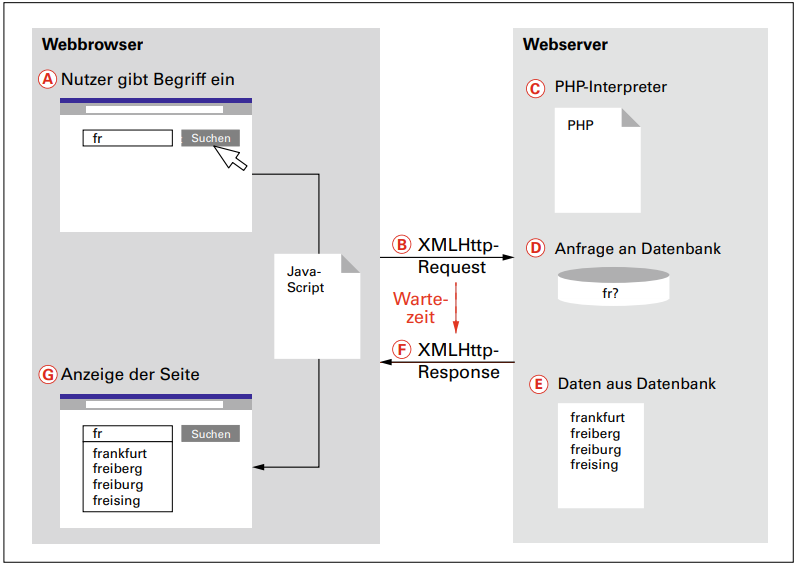
\includegraphics[scale=1.0]{images/AjaxUseCase}
	\caption{Anwendungsfall von Ajax, \cite{buhler2018webtechnologien}} 
	\label{img:/AjaxUseCase}
\end{figure}
Während ein User ein Textfeld beschreibt wird im Hintergrund, mithilfe des JavaScript-Objektes XMLHttpRequest, eine Anfrage an den Webserver gesendet. Dieser kann mit ersten Teilergebnissen antworten und so dem User bspw. eine Autovervollständigung anbieten. \ac{Ajax} ist in dem Fall keine neue Technologie sondert verwendet JavaScript anders, um mit dem Webserver im Hintergrund zu kommunizieren. In diesem Fall ist die Autovervollständigung lediglich ein einfaches Beispiel um die Funktion von \ac{Ajax} zu verstehen. Darüber hinaus gibt es weitaus mehr Anwendungsfälle von \ac{Ajax}. Bei aufwändigen Webseiten kommt ein weiteres Element zur Webentwicklung hinzu, das die Umsetzung erleichtern soll. Dabei handelt es sich um Frameworks. Wie es für \ac{CSS} und \ac{HTML} Bootstrap als Framework gibt, so gibt es auch im Zusammenhang mit JavaScript eine Vielzahl an Frameworks. Eines der beliebtesten Frameworks ist jQuery. Mit jQuery wird das Programmieren von JavaScript unterstützt. Außerdem ist der Zugriff auf HTML-Elemente bekannt durch die Varianten des Selektors bei \ac{CSS}. In jQuery wird über \$(\dq \#bereich1\dq) oder \$(\dq .farbe1\dq) auf ein Element zugegriffen. Der Standardaufbau, welcher in dem folgenden \autoref{lst:jQueryExample} dargestellt ist, zeigt eine Merkmal auf das zu achten ist.
\begin{lstlisting}[language=HTML,caption=Example Listing of jQuery,label={lst:jQueryExample}]
<script> $(document).ready(function(){
/* Hier der jQuery-Code */ });
</script>
\end{lstlisting}
Mit \texttt{\$(document).ready} werden grundsätzlich erste Probleme, die auftreten können verhindert. Demnach könnte ohne diese Funktion auf Elemente zugegriffen werden, welche noch nicht vollständig geladen sind. Das ready verhindert diese Problematik und wartet mit der Ausführung bis die Webseite komplett geladen ist. Die Problematik tritt sowohl bei jQuery als auch bei JavaScript auf. JQuery besitzt zahlreiche Plugins die bei der Webentwicklung verwendet werden können. JavaScript bildetet ein fundamentaler Baustein, der mithilfe zahlreicher Möglichkeiten und Frameworks für jede Anwendung Optionen bereitstellt, um dynamische Änderungen oder Interaktionen in die Webanwendung zu integrieren.\cite{buhler2018webtechnologien}
\pagebreak

\section{HTML und CSS-Entwicklung mit Hilfe von Bootstrap}
\label{sec:Bootstrap}
Im \autoref{sec:HTMLCSSJS} taucht der Begriff Bootstrap erstmalig auf. Herrn Krause zur Folge handelt es sich bei Bootstrap um ein \ac{CSS} Framework. In diesem Zusammenhang stellt sich die Frage, wieso der Titel des Abschnitts \ac{HTML} mit einbringt. Eine Frage welche im Verlauf des Abschnitts behandelt wird. Außerdem wird heutzutage ein Webauftritt durch zahlreiche Frameworks und Tools unterstützt, was die Relevanz des Abschnitts erklärt. Im Folgenden steht die Verwendung von Bootstrap und die hilfreichen Komponente, welche bei einer Webapplikation benutzt werden können, im Vordergrund. Hierbei handelt sich um zwei Komponenten deren Implementierung dargestellt werden. Weitere Kompontenten sind nicht Bestandteil der Ausführung, da sie aufgrund der Ähnlichkeit abgeleitet werden können. 

\subsection*{Installation und Integration von Bootstrap}
Bootstrap hat seinen Ursprung im Jahr 2010. Aufgrund der MIT Lizenz ist die Software frei zugänglich und erlaubt eine Wiederverwendung bei eigenen Projekten. Zum Zeitpunkt der Studienarbeit handelt es sich bei Bootstrap um die vierte Version (Bootstrap 4).\cite{bootstrapOnline}
Die Installation von Bootstrap unterschiedet sich von herkömmlichen Programmen, wie es ein unerfahrener Computernutzer gewöhnt ist. Bei Bootstrap handelt es sich um eine Vielzahl an Dateien, welche entweder über eine Online Verbindung eingebunden werden können, oder lokal. Bei der Online Verbindung muss lediglich die Quelle im entsprechenden Tag richtig gesetzt werden. Wird hingegen Bootstrap heruntergeladen, wird lokal ein Bootstrap-Ordner angelegt, der zahlreiche CSS-Dateien beinhaltet. Ein Übersicht über alle mitgelieferten Dateien ist in der \autoref{img:BootstrapStructer} dargestellt. Egal welcher Weg für die Integration von Bootstrap verwendet wird, die Webseite in Form der HTML-Datei muss mit den entsprechenden CSS-Dateien verknüpft werden.
\begin{lstlisting}[language=HTML,caption=Importieren der Bootstrap-Dateien,label={lst:IncludeBootstrap}]
<head>
<link rel="stylesheet"href="static/css/bootstrap.min.css') }}">
<link rel="stylesheet" href="static/css/font-awesome.min.css') }}">
</head>
\end{lstlisting}
Für die Integration gibt es mehrerer Möglichkeiten. Die wohl am häufigsten empfohlene Variante ist, die Integration im Header der HTML-Datei. Dafür wird, wie in dem \autoref{lst:IncludeBootstrap} dargestellt, innerhalb des head-Tags eine Referenz zur CSS-Datei von Bootstrap eingefügt. In diesem Fall handelt es sich um eine relative Referenz bei der die Dateien sich in dem entsprechenden Ordner befinden. \cite{krause2016introducing}

\subsection*{Wichtige Komponten und ihre Implementierung mithilfe Bootstrap}
\label{BootstrapComponents}
Mit dem Ziel Projekte bzw. Programme unabhängig von Betriebssystemen zu entwickeln, schieben sich die Webapplikationen immer mehr in den Vordergrund. Mit Hilfe von Bootstrap kann der Webauftritt komfortabel unterstützt werden. In diesem Abschnitt werden wichtige Komponenten und wie sie anzuwenden sind erörtert. Dadurch wird ein Basiswissen für Projekte welche als Webapplikation realisiert wird vermittelt. Aufgrund der Vielzahl an von Bootstrap angebotenen Möglichkeiten, werden ausschließlich die am häufigsten verwendeten Komponenten erläutert.

\textbf{Buttons}\\
Mit Bootstrap als CSS-Framework sind Komponenten wie Buttons in verschiedenen Formen bereits verfügbar. Das nachfolgende Listing (\autoref{lst:IncludeBootstrapButton}) bildet ab, wie ein vorgefertigter Button in eine HTML-Datei implementiert werden kann.
\begin{lstlisting}[language=HTML,caption=Implmentierung eines vorgerftigten Buttons,label={lst:IncludeBootstrapButton}]
<button class="btn btn-primary" type="submit">Button</button>
\end{lstlisting}
An dieser Stelle lässt sich die Frage nach der HTML-Verknüpfung, obwohl es sich um eine CSS-Framework handelt, beantworten. Die CSS-Dateien von Bootstrap definieren die Komponenten in ihrem gestalterischen Aspekt. An welcher Stelle und wie der Button zu verwenden ist, wird weiterhin mit \ac{HTML} oder \ac{JS} gelöst. Bei Betrachtung des Listings ist vor allem der Klassenname auffällig. Dieser ist bei einer eigenen Implementierung frei zu wählen. Wird aber eine Komponente von Bootstrap implementiert sind die spezifischen Namen zu verwenden, da zu diesem Namen eine Referenz in der CSS-Datei besteht.
\begin{figure}[h]
	\centering
	
\includegraphics[scale=2.1]{images/BootstrapButton}
	\caption{Darstellung eines Buttons durch Bootstrap, \cite{bootstrapOnline}} 
	\label{img:BootstrapButton}
\end{figure}
Nach erfolgreicher Implementierung kann ein Button, wie in \autoref{img:BootstrapButton} dargestellt, verwendet werden.

\textbf{Formulare}\\
Für einen Online-Händler ist das Formular nicht mehr wegzudenken. Doch auch bei Webapplikationen, die eine Registrierung bzw. eine Anmeldung verlangen benötigten in irgendeiner Form ein Formular. Hierfür kann eines mithilfe von Buttons und Inputs selbst implementiert werden oder ein Framework bringt Abhilfe. Im Fall von Bootstrap gibt es verschiedene Möglichkeiten eines Formulars. Für die Implementierung und Funktionsweise wird ein allgemeingültiges Formular betrachtet. Das \autoref{lst:IncludeBootstrapForm} stellt das Formular innerhalb der HTML-Datei dar.
\begin{lstlisting}[language=HTML,caption=Implmentierung eines Formulars \cite{bootstrapOnline},label={lst:IncludeBootstrapForm}]
<form>
<div class="form-group">
<label for="exampleInputEmail1">Email address</label>
<input type="email" class="form-control" id="exampleInputEmail1" aria-describedby="emailHelp">
<small id="Help" class="form-text text-muted">Helptext</small>
</div>
<div class="form-group">
<label for="exampleInputPassword1">Password</label>
<input type="password" class="form-control" id="exInpPwd">
</div>
<div class="form-group form-check">
<input type="checkbox" class="form-check-input" id="exampleCheck1">
<label class="form-check-label" for="Check1">Check me out</label>
</div>
<button type="submit" class="btn btn-primary">Submit</button>
</form>
\end{lstlisting}
Das Listing symbolisiert nicht nur das Formular sondern reflektiert die Verschachtelung einer HTML-Datei aus \autoref{sec:HTMLCSSJS}. Bestandteile dieses Listings, die nichts mit Bootstrap zu tun haben, sind:
\begin{itemize}
	\item HTML-Tags wie form, div, label, input, small
	\item Text innerhalb der HTML-Elemente
	\item Identifikationsnamen
\end{itemize}
Die Erkenntnis dieser Aufzählung zeigt, wie schlicht Bootstrap verwendet werden kann. Anderseits zeigt es wie aufwendig ein Formular auch mithilfe Bootstrap ist. Hier sei nochmals zu erwähnen, dass Bootstrap ausschließlich bei der Gestaltung unterstützt. Daher kann sind die HTML-Inhalte eigenständig zu implementieren. Dennoch kann mit Hilfe von Bootstrap ein Formular gestalterisch schnell umgesetzt werden. Das Resultat des Listings stellt die \autoref{img:BootstrapForm} dar. \cite{bootstrapOnline}
\begin{figure}[h]
	\centering
	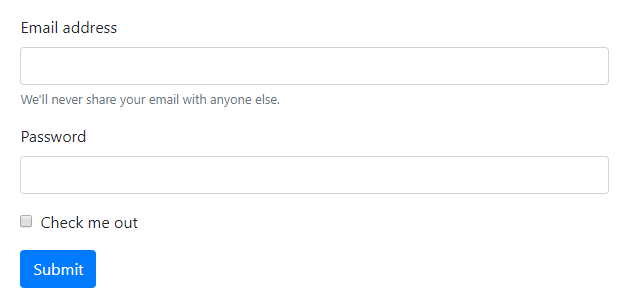
\includegraphics[scale=1.0]{images/BootstrapForm}
	\caption{Darstellung eines Formulars mit Bootstrap, \cite{bootstrapOnline}} 
	\label{img:BootstrapForm}
\end{figure}
\pagebreak

\chapter{Diskussion über die Art der Benutzeroberfläche}
\label{chap:DiskussionGUI}

Mit den theoretischen Inhalten aus \autoref{sec:Benutzeroberfläche} besteht Kenntnis über die Kernregeln einer grafischen Benutzeroberfläche. Um diese Regeln umzusetzen, sind vorab mehrere Aspekte, welche nachfolgend aufgeführt sind, zu beachten.
\begin{itemize}
	\item Programmiersprache
	\item Plattform
	\item Aufwand
\end{itemize}
Die Programmiersprache ist für jedes Projekt frei wählbar. Neben Vorteilen und Erfahrungen spielen persönliche Interessen ein großer Faktor bei der Wahl der Programmiersprache. Mit der Entscheidung über die Programmiersprache kann indirekt die Basis für eine grafische Benutzeroberfläche gelegt werden, je nachdem ob Backend und Frontend in der gleichen Programmiersprache sind. Aus diesen und weiteren Gründen wird in diesem Kapitel die Möglichkeiten einer grafischen Benutzeroberfläche mit der gewählten Sprache Python erörtert. Dabei spielt die Plattform ebenfalls eine wichtige Rolle. Diese definiert, wie und worauf der Benutzer das Programm nutzen kann. Welche Plattformen in Verbindung mit Python zur Verfügung stehen und welche, bezogen auf die Anforderungen aus \autoref{Anforderungen}, verwendet werden können, wird in den folgenden Abschnitten erörtert. Im Falle einer Entscheidung ist der Aufwand, in Form der Zeitspanne, ein wichtiges Kriterium, welches zu Diskussion beiträgt. Dieses Kriterium, bildet die Möglichkeit die Projektumsetzung mit den Projektanforderungen zu vergleichen. Bei der grafische Benutzeroberfläche nimmt das Kriterium Einfluss auf die Wahl eines Frameworks.

\section{GUI-Programmierung mit Python}
\label{sec:GuiPython}

Bei der Umsetzung einer grafischen Benutzeroberfläche müssen Regeln bezüglich der Usability (\autoref{sec:Benutzeroberfläche}) und die Eigenschaften der Programmiersprache beachtet werden. Mit Python als Programmiersprache kommen mehrere Module, welche für die grafische Benutzeroberfläche benutzt werden können, einher. Für diese Module ist vorab die Plattform zu wählen. Dabei geht es um die Diskussion, auf welche Plattform sich eine Chatapplikation mit Bezug zu den Nutzern besser realisieren lässt.

Die \ac{GUI}-Programmierung bei Python unterscheidet sich im Konzept nicht allzu sehr von anderen Programmiersprachen. Neben Schaltflächen stehen auch Fenster oder Menüs als Komponenten zur Verfügung. Angeordnet können diese in sogenannten Container. Für eine geeignete Anwenderschnittstelle müssen die Komponenten in die Container integriert werden. Hinzukommt ein äußerer Container, auch als Frame bezeichnet, ein Layout-Manager und eine Implementierung damit Aktionen durch Komponenten ausgelöst werden können. Wie im \autoref{sec:Benutzeroberfläche} erläutert, folgt eine \ac{GUI} mehreren Regeln. Demnach gibt es für die Programmierung einer grafischen Benutzeroberfläche vielerlei Möglichkeiten. In Python werden \ac{GUI} Frameworks angeboten, die eine Programmierung erleichtern sollen. Diese Frameworks können sich in der Art und der Verwendung unterscheiden. Außerdem sind Frameworks plattformabhängig. Damit ist eine Verwendung als Desktop- oder Webapplikation gemeint. Daher ist in der ersten Phase eine Plattform, anhand der Anforderungen an die Chatapplikation aus \autoref{Anforderungen}, zu evaluieren.\cite{Steyer2018}

\pagebreak

\autoref{tab:EntscheidungsmatrixFrameworkart} spiegelt die Ergebnisse eines Vergleichs zwischen den Tool-Frameworks und den Web-Frameworks von Python wider.

\renewcommand{\arraystretch}{2}
\begin{table}[h]
	\centering
	\caption{Entscheidungsmatrix der Frameworkart}
	\begin{tabular}{l|c|c|c}
		& & \multicolumn{2}{c}{Arten einer Python-GUI} \\
		Kriterien & Gewichtung & Tool-Framework & Web-Framework \\
		\hline
		Nutzerfreundlichkeit & 33\% & 2 & 2 \\
		\hline
		Schwierigkeit & 7\% & 2 & 1,7  \\
		\hline
		Umsetzbarkeit & 13\% & 2 & 2,2\\
		\hline
		Kompatibilität & 13\% & 2,2 & 1,7 \\
		\hline
		Design & 7\% & 2 &  2\\
		\hline 
		Verwendungszweck & 27\% & 2,5 & 1,5 \\
		\hline
		\textbf{Gesamtwertungszahl} & \textbf{100\%} & \textbf{2,161} & \textbf{1,831} \\
	\end{tabular}
	\label{tab:EntscheidungsmatrixFrameworkart}
\end{table}

Die Kriterien orientieren sich am Projekt und werden nachfolgend erläutert. Die Nutzerfreundlichkeit beinhaltet die Frage nach der Verständlichkeit. Dabei geht es darum, wie verständlich eine GUI mithilfe des Tools aufgebaut werden kann. Außerdem beinhaltet das Kriterium auch die Möglichkeiten des Tools, auf die Nutzerfreundlichkeit einzugehen. Die Schwierigkeit orientiert sich an der Implementierung. Dafür wird betrachtet wie leicht, schnell und komfortabel die Frameworkart in das Gesamtsystem integriert werden kann. Unabhängig von der Schwierigkeit geht es bei der Umsetzbarkeit um die Mittel, welche für eine Umsetzung benötigt werden, sowie auch um den Aufwand bei der Umsetzung. Die Kompatibilität umfasst die Unabhängigkeit von Betriebssystemen, Browsern und weitere Aspekte. Ein Standardkriterium für eine grafische Oberfläche ist das Design. Demnach geht es um die Möglichkeiten ein gutes Erscheinungsbild der Oberfläche mit dem entsprechenden Framework umzusetzen. Das letzte Kriterium, Verwendungszweck, bildet die Verbindung zum Projekt. Dafür wird analysiert, wie die Frameworkart zum Zweck des Projektes passt. Die Gewichtung der Kriterien innerhalb der \autoref{tab:EntscheidungsmatrixFrameworkart} sind der \autoref{tab:GewichtungFrameworkart} des Anhangs zu entnehmen.

Die \autoref{tab:EntscheidungsmatrixFrameworkart} bildet eine Hilfestellung zur Entscheidung einer passenden Frameworkart für das Projekt. Die Bewertung der Tools entsprechend der Kriterien folgt dem Benotungsschema der akademischen Bildung. Demnach ist eine 1 sehr gut und eine 6 ungenügend. Im Kriterium Nutzerfreundlichkeit schließen beide Frameworks mit der gleichen Note ab, da die Nutzerfreundlichkeit abhängig vom Designstil ist und bei beiden Frameworks umgesetzt werden kann. Das in der Einführung definierte Kriterium \glqq Schwierigkeit\grqq\, bekommt beim Web-Framework eine bessere Bewertung. Grund hierfür ist, dass für das Web-Framework überwiegend keine aufwändigen Module in Python benötigt werden. Gestaltet wird das Web Frontend über \ac{HTML} und \ac{CSS}, welche dann mit einem schlichten Modul verknüpft bzw. aufgerufen werden können. Aufgrund von Vorkenntnissen sowohl in \ac{HTML} als auch in \ac{CSS} wird die Schwierigkeit für das Web-Framework besser bewertet. Bei der Umsetzbarkeit steht das Tool-Framework aufgrund der Verwendung eines gesamten Moduls besser da. Ein Web-Framework bringt \ac{HTML}, \ac{CSS}, \ac{JS} und das Modul mit was ein größeren Umfang bedeutet. Vor allem muss der Programmierer mit allen Elementen umgehen können, weshalb eine Umsetzung schwieriger sein könnte. In der Kompatibilität wird das Web-Framework aufgrund der Unabhängigkeit bezüglich des Betriebssystems besser bewertet. Außerdem kann eine ausgelieferte \ac{HTML}-Seite von nahezu allen Browsern gelesen werden. Eine Möglichkeit die Lösung auf mobilen Endgeräten zu benutzen ist ebenfalls enthalten. Im Design unterscheiden sich die Frameworkarten nicht. Beide bieten vielerlei Möglichkeiten auf gestalterische Details einzugehen. Aufgrund des Projektes, einen Chat über \ac{XMPP} und ejabberd zu realisieren wird schon hauptsächlich das Internet genutzt. Dadurch bietet es sich an, den Server eine \ac{HTML}-Seite ausliefern zulassen. Aus diesem Grund wird das Web-Framework im Rahmen dieses Kriteriums besser bewertet. Anhand der Gesamtwertungszahl entsprechend der Benotung und der Gewichtung sind beide Frameworks zu empfehlen, dennoch schließt das Web-Framework besser ab, weshalb im weiteren Verlauf ein Web-Framework zum Einsatz kommen soll. \cite{FrameworkOverview} \cite{WebFramework}\\ 
Mit diesem Ergebnis müssen die verschiedenen Möglichkeiten eine Web-Framework in Bezug auf Python analysiert und bewertet werden. Auch in diesem Fall liefert eine Entscheidungsmatrix ein aufschlussreiches Ergebnis. Die Definition der selben Bewertungskriterien sind der Einführung der \autoref{tab:EntscheidungsmatrixFrameworkart} zu entnehmen. Weitere Kriterien wie Umfang und Komplexität werden in die Betrachtung miteinbezogen. Der Umfang spiegelt die Möglichkeiten und Größe im Aufbau des Tools wider. Die Komplexität befasst sich mit dem Aufwand einer Implementierung sowie auch die Hilfestellungen durch geeignete Dokumentationen. Das Bewertungsschema orientiert sich ebenfalls an der \autoref{tab:EntscheidungsmatrixFrameworkart}. Außerdem sind die Werte der Gewichtung bezogen auf das jeweilige Kriterium in der \autoref{tab:GewichtungWebFramework} im Anhang dargestellt.
\begin{table}[h]
	\centering
	\caption{Entscheidungsmatrix eines Web-Frameworks}
	\begin{tabular}{l|c|c|c|c|c}
		Kriterien & Gewichtung & Django & Flask & CherryPy & Bottle\\
		\hline
		Umfang & 17\% & 1,5 & 2 & 2 & 2,5 \\
		\hline
		Schwierigkeit & 17\% & 2,5 & 1,7 & 2,2 & 2 \\
		\hline
		Komplexität & 33\% & 2,2 & 1,7 & 2 & 1,7 \\
		\hline
		Verwendungszweck & 33\% & 2 & 2 & 2 & 2,2 \\
		\hline
		\textbf{Gesamtwertungszahl} & \textbf{100\%} & \textbf{2,067} & \textbf{1,850} & \textbf{2,033}  & \textbf{2,050} \\
	\end{tabular}
	\label{tab:EntscheidungsmatrixWebFramework}
\end{table}
Die Gesamtwertungszahl, welches der \autoref{tab:EntscheidungsmatrixWebFramework} entnommen werden kann, liefert ein knappes Ergebnis. Demnach bietet sich Flask am besten als Framework einer grafischen Oberfläche an. Im Umfang setzt sich das Tool Django gegen die Konkurrenten durch, da es aufgrund seiner Größe vielerlei Möglichkeiten mitbringt. Während die anderen Tools überwiegend als Mikroframework bezeichnet werden, zeichnet sich Django als Full-Stack/high-level Framework aus. Ebenfalls ein Grund weshalb die Schwierigkeit bei Django mit einer 2,5 bewertet ist. Ein Mikroframework bildet in der Hinsicht die leichtere und schnellere Variante. Die Komplexität ist vor allem bei Flask und Bottle gut bewertet. Grund hierfür ist unter anderem eine geringere Komplexität durch Möglichkeiten einer schlichten Implementierung. Außerdem bietet bspw. Flask eine sehr gute Dokumentation, welche die Komplexität verringern kann. Der Verwendungszweck ist nahezu gleichbleibend, da alle Frameworks genutzt werden können um das Projekt umzusetzen. Ausschließlich bei Bottle ist überwiegend die Rede von einem Framework das vor allem zur Einführung in das Themengebiet der Programmierung grafischer Oberflächen mit eine Web-Framework benutzt wird. Anhand des Ergebnisses und der sehr guten Dokumentation wird Flask als Web-Framework zum Einsatz kommen. Außerdem wird die Entscheidung durch die Statistiken aus dem Jahr 2018 (Abbildung) und dem Jahr 2020 (\cite{webframeworksStatistic}), in der Flask auch zu den beliebtesten Web-Frameworks zählt, unterstützt.
\cite{BottleDoc} \cite{CherryPyDoc} \cite{DjangoDoc} \cite{FlaskDoc}
\begin{figure}[h]
	\centering
	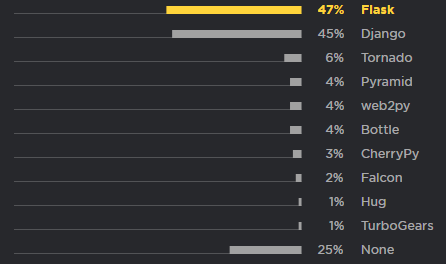
\includegraphics[scale=1.2]{images/FlaskSurvey2018}
	\caption{Ergebnis der Python Developers Survey 2018 \cite{pythonDeveloperSurvey2018}}
	\label{img:StatistikWebFrameworks}
\end{figure}

\section{Flask}
\label{sec:Flask}
Wie unter \autoref{sec:GuiPython} beschrieben, wird im Rahmen der Studienarbeit Flask verwendet. Es wird von mehreren Quellen und der offiziellen Dokumentation als Microframework betitelt. Grund hierfür ist der Aufbau von Flask. Bei der Definition des Begriffs \glqq micro\grqq\ ist nicht das Resultat zu betrachten. Mit Flask als Framework muss nicht die gesamte Web-Anwendung in einer Datei dargestellt werden. Hierbei handelt es sich eher um einen simplen Kern, welcher der Ausgangspunkt und das Ziel von Flask darstellt. Ausgehend von dem simplen Kern besitzt Flask die Möglichkeit in der Größe zu skalieren. Daher kann, bezogen auf die Grundstruktur von Flask, dem Begriff Framework das \glqq micro\grqq\ vorangestellt werden.\cite{FlaskDoc}\\
Auch Autoren, wie K. Relan mit seinem Werk über Flask und RESTAPIs, schmälern nicht die Funktionalität von Flask, sondern loben die simple Struktur mit der Erweiterbarkeit. Dadurch haben sie die Möglichkeit der Anwendung ihre eigene Konfiguration zuzuteilen und mit Erweiterungen leicht zu skalieren. \cite{FlaskRESTAPIsRelan}\\
Flask verknüpft die Entwicklung einer Web-Anwendung mit Python, weshalb das Framework eine Schnittstelle zum Webserver bildet. Bekannt ist Flask durch die Eigenschaft schnell und leicht eine minimale Anwendung zu implementieren und diese bei Bedarf in der Größe zu skalieren. Für die Verwendung von Flask sind zwei Bibliotheken wichtig. Bei diesen handelt es sich zum Einen um die \ac{WSGI}-Bibliothek Werkzeug und der Template-Bibliothek Jinja2. Module die standardmäßig von Flask verwendet werden. Flask bildet das Bindeglied zwischen den Modulen und erlaubt es bspw. mithilfe von Routen an bestimmten Endpunkten Funktionen, Aktionen oder ähnliches auszuführen. Ein Beispiel hierfür, wäre das ausliefern einer \ac{HTML}-Datei, welches im \autoref{lst:FlaskMinApp} dargestellt wird.
\begin{lstlisting}[language=Python,caption=Example Listing of Flask Python,label={lst:FlaskMinApp}]
from flask import Flask
app = Flask(__name__)

@app.route('/home')
def homepage():
return render_template('homepage.html')
\end{lstlisting}
Das \autoref{lst:FlaskMinApp} spiegelt das Routen sowie das Rendern einer \ac{HTML}-Datei von Python wider. Aufgrund des Paketverwaltungsprogramm pip kann Flask komfortabel installiert werden. Dementsprechend wird Flask in der ersten Zeile importiert, dann einer Anwendung zugeordnet und eine Route definiert. Dieser Route wird die Zeichenkette \glqq /homegrqq{} zugeteilt. Dadurch entstehen Vorteile auf Seiten der Betreiber als auch auf Seiten des Nutzers. Eine Route kann mithilfe des Browsers aufgerufen werden. In dem Fall der Anwendung aus dem \autoref{lst:FlaskMinApp}, läuft die Flask-Applikation auf der Adresse des localhost. Mit Aufruf des localhost (127.0.0.1) wird in der Flask-Applikation eine Route gesucht, welche auf die Anfrage eingeht. Dafür ergeben sich 3 Möglichkeiten, welche an dieser Stelle kurz erwähnt werden. Zum Einen kann der Browser zurückgeben, dass eine Webseite nicht erreichbar ist (\autoref{img:FlaskWebseiteNichtErreichabr}). 
\begin{figure}[h]
	\centering
	
\includegraphics[scale=1.5]{images/WebseiteNichtErreichbar}
	\caption{Keine Erreichbarkeit der Webseite, eigene Darstellung}
	\label{img:FlaskWebseiteNichtErreichabr}
\end{figure}
In dem Fall kann es sein, dass die Flask-Applikation nicht aktiv ist oder auf einer anderen Adresse erreichbar ist. Auch ein Netzwerkproblem könnte die Ursache hierfür sein. Bei der zweiten Möglichkeit befindet sich in der Flask-APP keine Route für die angegebene Adresse.
\begin{figure}[h]
	\centering
	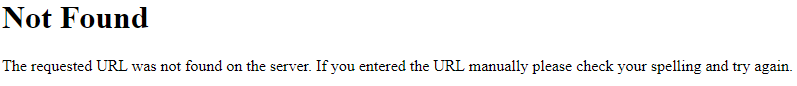
\includegraphics[scale=1.0]{images/NotFound}
	%TODO Ändern der Caption?
	\caption{Keine Erreichbarkeit der Webseite, eigene Darstellung}
	\label{img:FlaskWebseiteNotFound}
\end{figure}
In dem Fall kommt eine 404 mit der Bemerkung, dass die URL nicht gefunden wird, zurück (\autoref{img:FlaskWebseiteNichtErreichabr}). Bei der letzten Möglichkeit handelt es sich um eine korrekte URL. Im Fall des Beispieles wäre die Adresse: \texttt{http://127.0.0.1:8000/home} eine im \autoref{lst:FlaskMinApp} dargestellte Route. Durch den Aufruf der URL wird die definierte Funktion ausgeführt. Bei dem Beispiel wird eine HTML-Datei ausgeliefert.
Nun besitzt Flask vielerlei Möglichkeiten um Anfrage (POST, GET, usw.) zu differenzieren. Diese zählen nicht zur Grundfunktionalität von Flask und sind daher nicht Bestandteil dieses Abschnittes. Der nächste Vorteil von Flask beinhaltet die Möglichkeit einen Webserver im Entwicklungsmodus zu starten und aktuelle Code-Zeilen zu testen.
Flask ist also nicht zuständig für die Gestaltung der grafischen Oberfläche sondern benutzt sogenannte Templates in Form von HTML-Datei, die eine Webseite aufbauen. Für eine dynamische Webanwendung und den gestalterischen Aspekten sind statische Dateien, wie z.B. \ac{CSS}, notwendig. Aus diesem Grund benötigt Flask eine vorgegebene Ordnerstruktur, welche der nachfolgenden \autoref{img:TreeFlaskOrdnerstrukt} entnommen werden kann. Diese Struktur hilft um das Fehlerpotential, ausgelöst durch Zugriffe auf falsche Dateien, zu vermindern.
\begin{figure}[h]
	\centering
	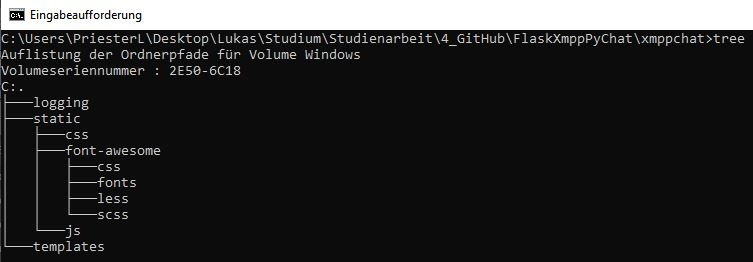
\includegraphics[width=\textwidth]{images/TreeFlaskOrdnerstrukt}
	\caption{Ordnerstruktur unter Flask, eigene Darstellung}
	\label{img:TreeFlaskOrdnerstrukt}
\end{figure}
Für die grafische Benutzeroberfläche würden diese Elemente ausreichen um eine simple Webseite aufzubauen, mit den \ac{HTML}- und \ac{CSS}-Dateien zu verknüpfen, über eine Route die Seite zu rendern und letztendlich, über den von Flask gestellten Webserver, zu testen. Dennoch bietet Flask mehr Möglichkeiten auch im Zusammenhang des Projektes. Zum Beispiel kann in Flask mit redirects, sessions, cookies, Datenbanken und vieles mehr gearbeitet werden. Bei der Anbindung bzw. Kommunikation mit einer Datenbank schreibt Flask als Modul nicht die Art der Datenbank vor. Dadurch gibt es die Möglichkeit bspw. eine MySQL, PostgreSQL, SQLite oder andere Datenbanken zu verwenden. In diesem Zusammenhang bietet Flask das Modul Flask-SQLAlchemy. Das Paket gilt als \ac{ORM}, und bietet die Möglichkeit high-level Operationen in Datenbank-Kommandos zu übersetzen. Ein Beispiel für die Verwendung des Moduls ist im folgenden \autoref{lst:SQLAlchemyMinApp} dargestellt.
\begin{lstlisting}[language=Python,caption=Example Listing of Flask-SQLAlchemy,label={lst:SQLAlchemyMinApp}]
from flask import Flask
from flask_sqlalchemy import SQLAlchemy

app = Flask(__name__)
app.config['SQLALCHEMY_DATABASE_URI'] = 'sqlite:////tmp/test.db'
db = SQLAlchemy(app)

class User(db.Model):
id = db.Column(db.Integer, primary_key=True)
username = db.Column(db.String(80), unique=True, nullable=False)
email = db.Column(db.String(120), unique=True, nullable=False)

def __repr__(self):
return '<User %r>' % self.username
\end{lstlisting}
Das Listing zeigt eine minimale Anwendung, welche die Erweiterung für die Datenbank nutzt. Dadurch bietet sich für den Programmierer, nach importieren alle nötigen Klassen, Benutzer ohne großen Aufwand herzustellen und der Datenbank hinzuzufügen (\autoref{lst:SQLAlchemyAddUser}).
\begin{lstlisting}[language=Python,caption=Hinzufügen eines Objektes in die Datenbanktabelle,label={lst:SQLAlchemyAddUser}]
>>> from yourapplication import User
>>> admin = User(username='admin', email='admin@example.com')
>>> guest = User(username='guest', email='guest@example.com')
\end{lstlisting}
Diese Listings zeigen nur einen Ausschnitt welche Möglichkeiten das Web-Framework bietet. Das ist der Grund für die Verwendung von Flask.\cite{FlaskDoc}
\pagebreak

\chapter{Verprobung eines Einsatzes von Kafka und Ejabberd in einem Messaging System}
\label{chap:VerprbungIMS}

Estrada und Ruiz sind der Meinung, das heutzutage kontinuierlich Echtzeitinformationen generiert werden \cite{estradaRuiz2016}. Die Daten müssen schnell und auf einfache Weise zu ihren Empfängern geliefert werden. Nach der Ansicht von Estrada und Ruiz \cite{estradaRuiz2016} sind Systeme, die Informationen produzieren (englisch Producer), und die Systeme, die Informationen konsumieren (englisch Consumer), untereinander unzugänglich. Berle \cite{berleKafkaOverview} weist auf Herausforderungen hin, die bei einem Versand von Nachrichten von einem System A an System B vorhanden sind, wenn diese direkt über \acs{RMI}\footnote{\ac{RMI} bezeichnet einen Aufruf eines entfernten Objekts und unterscheidet sich von einem \ac{RPC} nur darin, dass durch eine lokale Prozedur ein Objekt statt einer Anwendung aufgerufen wird.\cite[S.41]{andrew2008verteilte}}, einer \acs{REST} \acs{API} oder über Sockets miteinander kommunizieren, siehe \autoref{img:directCommunication}.

\begin{figure}[h]
	\centering
	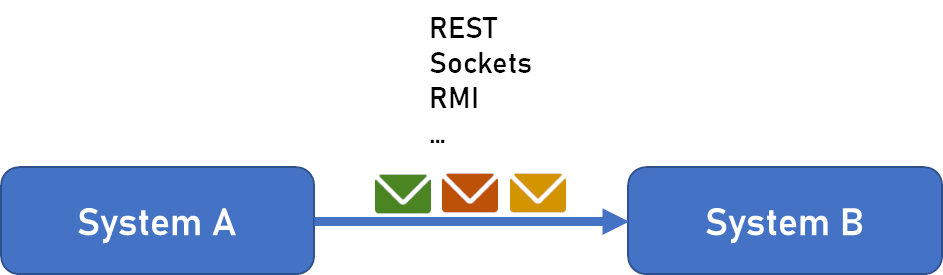
\includegraphics[width=.8\linewidth]{images/directCommunication}
	\caption{Direkte Kommunikation zwischen einem System A und System B, eigene Darstellung}
	\label{img:directCommunication}
\end{figure}

\subsubsection*{Herausforderungen der direkten Kommunikation\cite{berleKafkaOverview}:}

\begin{itemize}
\item System B ist aufgrund eines Wartungsfensters oder Netzwerkfehlers nicht erreichbar. System A hat aber nicht die Kapazität, Nachrichten so lange zu puffern, bis System B wieder verfügbar ist.
\item System A kann System B überlasten, indem A mehr Nachrichten schickt als B verarbeiten kann (\ac{DOS} Attacke).
\item System B erhält eine Nachricht von System A und stürzt während der Verarbeitung ab. Für System A gilt die Nachricht als verarbeitet, obwohl das nicht der Fall ist.
\end{itemize}

Um die Probleme lösen zu können, werden nach Berle Messaging Systeme zwischen Sender und Empfänger platziert, siehe \autoref{img:messagingSystemsCommunication}.

\begin{figure}[h]
	\centering
	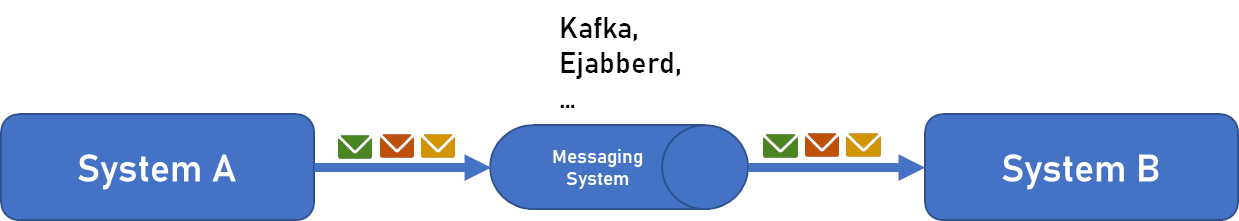
\includegraphics[width=\linewidth]{images/messagingSystemsCommunication}
	\caption{Kommunikation von System A und B über ein Messaging System, eigene Darstellung}
	\label{img:messagingSystemsCommunication}
\end{figure}

Konkreter kommen sogenannte Broker, auch Message Broker genannt, zum Einsatz. Ein Broker ist nach \cite{kimmerBroker} eine Einrichtung zur Vermittlung von Nachrichten zwischen einem Sender und einem oder mehreren Empfängern. Typische Aufgaben eines Message Brokers sind \cite{kimmerBroker}:

\begin{itemize}
\item Empfang und Versand von Nachrichten
\item Übersetzung des Nachrichtenformates des Senders in ein oder mehrere Nachrichtenformate des oder der Empfänger
\item Sorgt für effiziente Nachrichtenvermittlung (priorisierbare Nachrichtenverarbeitung)
\item Verbindung heterogener Systeme
\end{itemize}

Eine andere Möglichkeit ist ein Instant Messaging Server wie ejabberd. Nachrichten werden dabei über ein spezielles Protokoll - \ac{XMPP} (siehe \autoref{sec:XMPP}) - versendet. Ejabberd hat ähnliche Aufgaben wie ein Broker, nur dass alle Clients \acs{XMPP} als gemeinsame Sprache verstehen müssen, um miteinander kommunizieren zu können.

Auf diese Weise ist es Entwicklern möglich, skalierbare Systeme zu entwickeln, die eine Vielzahl von Benutzern unterstützen. Die meisten Messaging Systeme lassen sich in einem Cluster aufbauen, sodass die Last über mehrere identische Komponenten verteilt werden kann. Im Gegensatz zu Methoden wie \ac{RMI} muss ein Client nicht dauerhaft erreichbar und aktiviert sein \cite{andrew2008verteilte}. Das Broker System oder der Instant Messaging Server verwalten die Nachrichten des Clients und stellen die Nachrichten dem Client erst zu, wenn dieser wieder aktiv wird.

Sowohl ejabberd als auch Apache Kafka eignen sich, um Berles aufgeführten Probleme zu lösen. In der Studienarbeit werden beide Plattformen in ein eigenes \ac{IMS} integriert und für den Transport, die Verwaltung und die Speicherung von Nachrichten verwendet. Beide sollen auf Eignung überprüft werden und die Performanz der beiden Systeme verglichen werden.

\pagebreak


\chapter{Aufbau und Entwurf der Architektur des Chatsystems}
\label{chap:Architektur}

Nach den Anforderungen (\autoref{Anforderungen}) und Zielen der Arbeit (\autoref{sec:Ziele}) soll ein \ac{IMS} auf Basis eines \ac{XMPP}-Chatsystems entworfen und programmiert werden. Anschließend soll das gleiche Chatsystem auf Basis der Technologie Apache Kafka implementiert und mit dem \ac{XMPP}-Chatsystem verglichen werden. Hierfür muss ein verteiltes System entworfen werden.

Der Autor Tanenbaum definiert ein verteiltes System wie folgt: \glqq Ein verteiltes System ist eine Ansammlung unabhängiger Computer, die den Benutzern wie ein einzelnes kohärentes System erscheinen.\grqq\ \footnote{\cite[S.19]{andrew2008verteilte}} Die Definition von Tanenbaum hat mehrere wichtige Aspekte. Der Erste besagt, dass ein verteiltes System aus Komponenten besteht, die autonom sind. Sie bieten einen Dienst an oder haben eine bestimmte Aufgabe und eine lokale Zeit. Ein zweiter Aspekt ist, dass die Benutzer glauben, sie hätten es mit einem einzigen System zu tun. Die Eigenschaft \glqq kohärenz\grqq\ aus der Definition besagt, dass die Komponenten in einer bestimmten Art und Weise zusammen arbeiten, um den Benutzer einen Dienst zu erbringen. Ein besonderes Merkmal ist, dass keinerlei Annahmen über die Art der Computer getroffen werden. Diese können heterogen sein. Tanenbaum \cite{andrew2008verteilte} ist der Ansicht, dass die Herausforderungen eines verteilten Systems sind, die einzelnen Teilsysteme zu synchronisieren und die Zusammenarbeit korrekt zu implementieren.

Hierzu stellt sich die Frage, welche Dienste für das Chatsystem benötigt und wie die Dienste auf Komponenten sinnvoll verteilt werden. Der erste Teil der Frage kann mit Hilfe der Anforderungen aus \autoref{Anforderungen} beantwortet werden. Folgende Auflistung beinhaltet wichtige Funktionalitäten die als Komponenten zusammengefasst sind:

\begin{itemize}
\item Client für Benutzer, um Chat-Funktionalitäten durchführen zu können
\item ejabberd als \ac{XMPP}-Server für das \ac{XMPP}-basierte Chatsystem
\item Apache Kafka
\item Datenbank für Authentifizierung und Archivierung von Nachrichten
\end{itemize}

\newpage

Für die Beantwortung der Fragestellung, wie die Dienste auf Komponenten verteilt werden, bedarf es noch weiteren Untersuchungen. Theoretisch könnten alle Dienste bis auf den Chat-Client auf einer einzelnen Server-Instanz realisiert werden. Ein Vorteil ist, dass einzelne Dienste ohne Netzwerklatenzen miteinander kommunizieren können und Daten direkt austauschen können. Latenzen entstehen dann nur bei der Übertragung von Nachrichten vom Server zum Chat-Client und umgekehrt oder aufgrund der Bearbeitungszeit eines Dienstes. Dieser Architektur ist kritisch anzumerken, das die einzelnen Dienste um Ressourcen konkurrieren könnten und die Funktionsfähigkeit stark von der Qualität und der Leistung des Servers abhängig ist. Hinzu kommt, dass wenn der Server ausfällt oder beschädigt wird, jeder Dienst nicht mehr erreichbar ist. Das wäre entgegen den Vorteilen und Absichten von verteilten Systemen. Um die Architektur zu verbessern müssen die Eigenschaften und Ziele von verteilten Systemen berücksichtigt werden. Tanenbaum geht darauf detailliert in \cite{andrew2008verteilte} ein.

\subsubsection*{Eigenschaften von verteilten Systemen}

Eine Eigenschaft ist, dass die Unterschiede der Komponenten und die Art, wie sie untereinander kommunizieren, weitestgehend vor den Benutzern verborgen bleiben. Das bedeutet, dass wenn ein Benutzer eine Nachricht zu einem anderen Benutzer über das \ac{IMS} sendet, darf ein Benutzer nicht mitbekommen, wie viele und welche Instanzen mitwirken, um die Nachricht ihrem Empfänger zuzustellen. Eine weitere wichtige Eigenschaft ist, dass Benutzer konsistent mit dem verteilten System arbeiten können, egal wo und wann diese Zusammenarbeit stattfindet. Die Tatsache, dass ein Benutzer am \ac{IMS} angemeldet ist und Nachrichten versendet, darf keine Aktionen anderer Benutzer beeinflussen. Darüber hinaus sollte es leicht erweiterbar und skalierbar sein. Dieser Aspekt ist in dem vorher beschrieben Ansatz nicht gegeben. Es können nicht beliebig viele Dienste auf einem Server realisiert werden und auch die Ressourcen eines einzelnen Servers können nicht beliebig erweitert werden. Ein weiterer Punkt ist,dass Benutzer und Anwendungen nicht bemerken sollen, dass Teile ersetzt, repariert oder neue Teile hinzugefügt werden, um mehr Benutzer oder Anwendungen bedienen zu können.\cite{andrew2008verteilte}
Auf den Aspekt der Redundanz wird in dieser Arbeit nicht eingegangen. Das Ziel ist es nicht die Fehlertoleranz durch redundante Komponenten und Anwendungen zu gewährleisten, vielmehr soll ein Prototyp mit ausreichenden Funktionalitäten eines \ac{IMS} entwickelt werden und zwei verschiedene Implementierungsformen verglichen werden.

\subsubsection*{Ziele von verteilten Systemen \cite{andrew2008verteilte}}

\begin{itemize}
\item Ein verteiltes System sollte Ressourcen leicht zugreifbar machen.
\item Es sollt die Tatsache vernünftig verbergen, dass Ressourcen über ein Netzwerk verteilt sind.
\item Es sollt offen sein.
\item Es sollte skalierbar sein.
\end{itemize}

Die Auflistung führt Ziele auf, die Tanenbaum \cite{andrew2008verteilte} in seinem Werk immer wieder betont. Diese sind in Bezug auf das zu entwerfende \ac{IMS} wie folgt zu interpretieren:

Die Ressourcen sind die Chat-Funktionalitäten die ein Benutzer wahrnehmen kann. Das entwickelte System sollte diese Funktionalitäten dem Benutzer einfach zugänglich machen. Einfach zugänglich machen bedeutet, dass ein Benutzer nicht manuell sämtliche Dienste über viele Anmeldungen aufrufen muss, damit eine Nachricht an einem anderen Benutzer versendet wird. Vielmehr soll das \ac{IMS}, nachdem der Benutzer einen zentralen Auftrag zum Senden einer Nachricht veranlasst hat, alle benötigten Dienste selbst ansteuern und die Nachricht zuverlässig versenden. Ob und wie viele weiteren Dienste hierfür benötigt werden, soll das System vor dem Benutzer verbergen. Diesen Sachverhalt bezeichnet Tanenbaum in \cite{andrew2008verteilte} als Verteilungstransparenz. Das System muss also verbergen, dass es mit einer Datenbank oder mit ejabberd kommunizieren muss, um die Nachricht dem Empfänger zu zustellen. Neumann  definiert Skalierbarkeit sehr ausführlich in \cite{neumannDistributed1994}. Neumann ist der Auffassung, dass ein verteiltes System, das hinsichtlich seiner Ausdehnung skaliert wird, nicht an Leistung verlieren darf. Konkret für das \ac{IMS} bedeutet das, das durch ein Hinzufügen oder Duplizieren von Diensten andere Teilsysteme nicht negativ beeinflusst werden dürfen. Neumann betont, dass es nicht sinnvoll ist, einen Dienst nur zentral auf einem Server bereitzustellen. Nach seiner Meinung können Server einer zentralisierten Architektur zum Engpass werden. Diese Ansicht ist zutreffend, wenn das \ac{IMS} als Produktivsystem entwickelt werden würde. Das ist aber in dieser Studienarbeit nicht der Fall und kann deshalb vernachlässigt werden.

Das Ergebnis der Diskussion aus \autoref{chap:DiskussionGUI} bestätigt, das sich für die Art der Anwendung eine Webanwendung besonders eignet. Das erfordert, das der Benutzer mit dem \ac{IMS} direkt über den Browser interagieren kann. Die Webanwendung setzt allerdings eine Anwendungslogik voraus, die die Aktionen des Benutzers koordiniert und kontrolliert. Um das Gesamtsystem flexibel zu halten, sodass neben einem Benutzer auch andere Webdienste mit dem \ac{IMS} interagieren können, wird eine \acs{REST} \acs{API} programmiert. \acs{REST} bezeichnet einen Architekturstil, den Roy Fielding in seiner Dissertation \cite{fieldingREST} aus dem Jahr 2000 beschreibt. \ac{REST} verspricht Wiederverwendbarkeit, Erweiterbarkeit, Skalierbarkeit und die einfache Integration in die vorhandene Netz-Struktur \cite{fieldingREST}. Ressourcen werden über \acs{URI}s und über einen eindeutigen Namen aufgerufen. Die Ressourcen können in unterschiedlicher Form auftreten, wie zum Beispiel: \acs{PDF}, \acs{XML}, \acs{JSON} als moderne Form oder \acs{HTML}. Die Tatsache, dass eine Nachricht eines Benutzers über einen Aufruf einer \acs{URI}, wie zum Beispiel \texttt{https://chatportal.de/send-message}, von einem Client beauftragt werden kann, bestätigt die Vorteile des Architekturstils. Kommen in ferner Zukunft weitere Möglichkeiten für den Versand einer Nachricht hinzu, muss nur eine neue \acs{API}-Route eingerichtet werden. Das System bleibt flexibel und erweiterbar. Aus diesen Gründen wird für die Anwendungslogik eine \acs{REST} \acs{API} mit dem Framework Python Flask entwickelt.

Beachtet man die oben aufgeführten Überlegungen, ergibt sich für die Architektur die in \autoref{img:logischeTopologieIMS} dargestellte logische Topologie.

\begin{figure}[h]
	\centering
	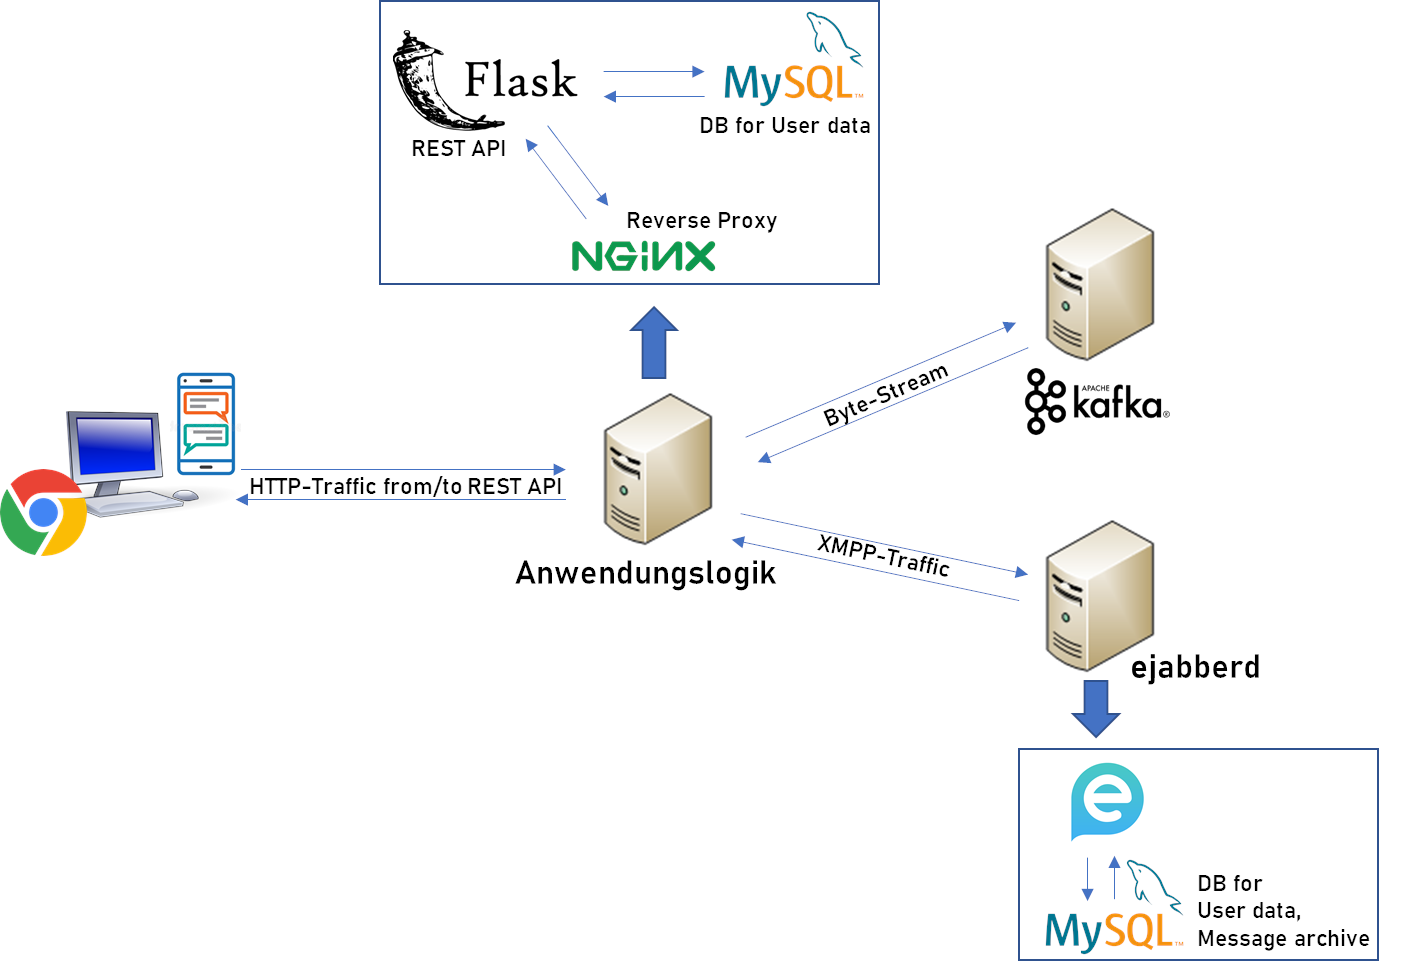
\includegraphics[width=\linewidth]{images/DetailliertesIMSArchitecture}
	\caption{Logische Topologie des zu entwickelnden \ac{IMS}, eigene Darstellung}
	\label{img:logischeTopologieIMS}
\end{figure}

Jeder Dienst wird auf einem Server verteilt mit Ausnahme der Datenbanken. Ejabberd und Kafka bilden die beiden unterschiedlichen Plattformen über die Chat-Nachrichten versendet werden können. Die Instanz zwischen den Clients und den beiden Plattformen realisiert die Anwendungslogik in Form einer \acs{REST} \acs{API}, die mit dem Microframework Python Flask entwickelt wird.

Die Grundidee ist folgende: Über ein Web-Frontend werden dem Benutzer Chat-Funktionalitäten bereitgestellt, die er nach einer Anmeldung am System verwenden kann. Über das Web-Frontend kann der Benutzer auswählen, ob er über den Apache Kafka Dienst oder über ejabberd Chat-Dienste nutzen möchte. Das Web-Frontend erzeugt hierzu entsprechende Requests, um der Flask Applikation mitzuteilen, für welche der beiden Plattformen sich der Benutzer anmeldet. So können beide Plattformen getrennt voneinander getestet werden. Ist ein Benutzer am \ac{IMS} angemeldet, werden die Nachrichten ausschließlich zu dem Dienst, für den sich der Benutzer zuvor angemeldet hat, koordiniert. Eine Benutzung von Apache Kafka und Ejabberd via \ac{XMPP} ist gleichzeitig nicht möglich. Die Architektur ist so entworfen, dass die \acs{REST} \acs{API} die volle Kontrolle über die Dienste für den Nachrichtentransport verfügt und alle Anfragen der Clients verarbeitet. Eine Kommunikation von Clients zu den Chat-Diensten direkt ist durch bestimmte Firewall-Regeln ausgeschlossen. Ein Client versendet und empfängt Nachrichten immer über die \acs{REST} \acs{API}. Aus Gründen des Qualitätsanspruchs werden Kafka und die ejabberd-Instanz trotzdem so konfiguriert, dass sie auch ohne der Anwendungslogik vollständig über das Internet benutzbar wären.

Wie die Anwendungslogik detailliert arbeitet, ist in der Detailansicht innerhalb von \autoref{img:logischeTopologieIMS} gezeigt (siehe blaue Rahmen). Zwischen den Clients und der Flask Applikation befindet sich NGINX als Reverse Proxy. Nach \cite{reverseProxyDesc} ist ein Reverse Proxy eine zusätzliche Schutzmaßnahme, die vor einen oder mehreren Webservern geschaltet werden kann. Im Gegensatz zu einem Proxy wird die Adressumsetzung in der entgegengesetzten Richtung durchgeführt.
Die Aufgabe des Reverse Proxys ist es, Anfragen von Clients stellvertretend anzunehmen und an den entsprechenden Server weiterzuleiten \cite{reverseProxyDesc}. Auf das \ac{IMS} bezogen, leitet NGINX Anfragen von Clients an die Flask \acs{REST} \acs{API} weiter. Die Flask Applikation benutzt eine MySQL Datenbank für die Benutzerauthentifizierung. Sie überprüft bei einer Anmeldung, ob der Benutzer berechtigt ist, das \ac{IMS} zu verwenden oder legt auf Anfrage einen neuen Benutzer in der Datenbank an. Zusätzlich versendet sie je nach gewählter Chat-Plattform des Benutzers, Nachrichten über \ac{XMPP} an ejabberd oder über Byte-Streams an Apache Kafka. Umgekehrt stellt sie dem Client die Nachrichten über eine Schnittstelle zu. Um Nachrichtenverläufe einem Client zu übermitteln, der das \ac{IMS} über ejabberd nutzen möchte, benötigt die \acs{REST} \acs{API} Zugang zur MySQL-Datenbank des ejabberd-Servers. Ejabberd benötigt eine eigene Datenbank, in der er Benutzer und Nachrichtenverläufe verwaltet. Er könnte auch alleine als \ac{IMS} mit Clients interagieren. Für die Integration von ejabberd in das selbst entwickelte \ac{IMS} können die beiden Datenbanken nicht zusammengeführt werden, weil für die Tabelle, in der Benutzerdaten gespeichert werden, keine Beschreibung in der ejabberd-Dokumentation vorhanden ist. Es sind keine Informationen über den verwendeten Hash-Algorithmus und wie der Salt erzeugt wird, enthalten. Der Aufwand der Synchronisation der beiden Datenbanken ist geringer, als den Code der open source Plattform ejabberd zu verstehen und die Algorithmen zu identifizieren. Die Konfiguration von ejabberd so zu verändern, dass die Passwörter in Klartext gespeichert werden, wird nicht den Zielen und dem Anspruch an diese Studienarbeit gerecht. Aus diesem Grund muss die \acs{REST} \acs{API} einen neuen Benutzer in beiden Datenbanken anlegen und die Benutzertabellen synchronisieren.

Abbildung \autoref{img:ArchitekturIMS} im Anhang zeigt die Netzwerktopologie des \ac{IMS}. Der ejabberd-Server ist in \autoref{img:ArchitekturIMS} als \texttt{ejabberd01} gekennzeichnet und der Apache Kafka Dienst als \texttt{apkafka01}. Die Instanz \texttt{ims-webapp01} realisiert NGINX, die Flask Applikation und die MySQL-Datenbank für Benutzerdaten. Auffällig ist, dass alle drei Instanzen eine öffentliche IP-Adresse im Internet haben. Der Internetzugang ist über eine Firewall gesichert und dient der Erreichbarkeit der Geräte für Debugging oder administrative Zwecke. Beispielsweise um über das \ac{SSH} Protokoll Software-Installationen durchzuführen oder Konfigurationen zu verwalten.

Diese Architektur ist unempfindlich gegenüber Erweiterungen. Würden in der Zukunft weitere Plattformen hinzukommen, müssen nur neue \acs{API}-Endpunkte hinzugefügt werden und die neuen Funktionen im Code umgesetzt werden. Bestehender Code und Endpunkte müssen nicht verändert werden. Zudem kann eine Komponente einfach ausgetauscht werden, falls diese beschädigt wird. Solange die Konfiguration die Gleiche bleibt, muss die Anwendungslogik nicht angepasst werden.

Nachdem die Architektur nach den Aspekten eines verteilten Systems entworfen ist, wird in den nächsten Kapiteln die Umsetzung der Architektur beschrieben. In den folgenden Abschnitten werden zuerst die Installation und Konfiguration von ejabberd und von Apache Kafka beschrieben. Danach wird die Umsetzung der Anwendungslogik in Python Flask erläutert und anschließend detailliert auf die Implementierung des Frontends eingegangen. Dabei werden wichtige Herausforderungen und deren Lösungsmöglichkeiten diskutiert.

\pagebreak

\chapter{Ejabberd als moderner Chatserver}
\label{chap:ejabberd}

Ejabberd ist einer der bekanntesten \ac{XMPP}-Server auf der Welt und kann in vielerlei Hinsicht verwendet werden. Er ist lizenzfrei benutzbar und unterstützt das Betriebssystem Windows, Linux und Mac OS. Sowohl Großprojekte als auch kleine Instanzen machen sich die Eigenschaften von ejabberd zum Vorteil. Der Start von ejabberd ist dem Jahr 2002 zuzuordnen. Ejabberd ist eine Abkürzung und steht für \glqq Erlang Jabber Daemon\grqq. Wie die Definition zeigt bezieht sich ejabberd auf die Programmiersprache Erlang. Grund hierfür ist, dass die ejabberd Software in Erlang geschrieben ist. Ejabber ist von Grund auf für die Unternehmensbereitstellung entwickelt, vor allem mit dem Ziel robust zu sein. Aufgrund davon, dass der Fokus auf die Unternehmen liegt, ist es wichtig, die Fehleranfälligkeit von ejabberd zu minimieren. Ein Vorteil der sich bis zum heutigen Zeitpunkt bewahrt hat. Außerdem kann ejabberd die Ressourcen mehrerer geclusterter Systeme nutzen. Des Weiteren besitzt ejabberd die Eigenschaft der Skalierbarkeit, indem die Kapazitäten mit wenig Aufwand erhöht werden kann. Ejabberd kann verschieden benutzt werden. Im Fall der Studienarbeit wird die Community Edition von ejabberd benutzt, welche als open source zur Verfügung steht. Neben der Community Edition gibt es auch noch Möglichkeiten einer Business Edition, welches vor allem für die großen Unternehmen mit besserem Support und mehr Funktionen konzeptioniert ist. Die Architektur eines ejabberd-Services erweitert die Kernfunktionen von \ac{XMPP}, welches das Senden von Nachrichten ist, um Faktoren wie die Skalierbarkeit, Konfigurierbarkeit und Fehlertoleranz.

\bigskip

\textbf{Relevante Funktionen:}

\begin{itemize}
	\item Einzelchat
	\item Gruppenchat (auch als Multi-User-Chat (\ac{MUC}) bezeichnet)
	\item Offline Nachrichten 
	\item Web-Unterstützung
	\item Nachrichtenübermittlungsbestätigung
	\item Übermittlung des Online-Status
	\item Verschlüsselte Übertragung von Nachrichten
	\item Kontaktliste jedes Benutzers
\end{itemize}

Die Architektur von ejabberd ist modular. Das bedeutet, dass die Architektur an den Zweck eines Projektes angepasst werden kann.

\autoref{img:ArchitekturEjabberd} zeigt eine Übersicht über die Architektur und die Flexibilität von ejabberd \cite{ejabberdModulesDeployment}.

\begin{figure}[h]
	\centering
	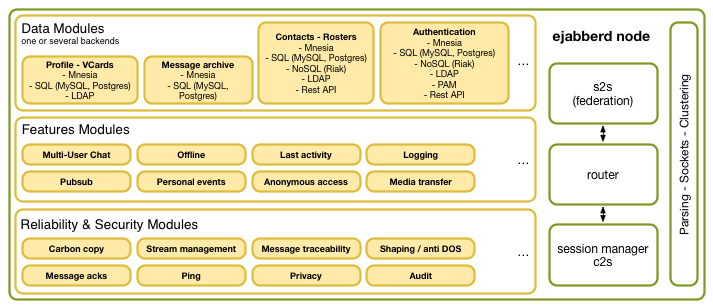
\includegraphics[width=\linewidth]{images/ejabberd_internals}
	\caption{Übersicht über die Architektur von ejabberd \cite{ejabberdModulesDeployment}}
	\label{img:ArchitekturEjabberd}
\end{figure}

Die interne Architektur von ejabberd setzt auf dem Router auf. Der Router leitet Anfragen an interne Dienste und Module weiter oder versendet Nachrichten. Neben der Kommunikation zwischen Clients und Server (c2s) unterstützt ejabberd die Kommunikation zu anderen \ac{XMPP}-Servern (s2s) und kann in bereits vorhandenen \ac{XMPP}-Domänen integriert werden. Die meisten anderen Elemente sind Plugins, die angepasst, erweitert oder ersetzt werden können, um eine benutzerdefinierte Lösung zu erstellen, die auf konkrete Anforderungen zugeschnitten ist. So lassen sich zum Beispiel Funktionen wie \ac{MUC} oder Logging benutzerdefiniert konfigurieren, siehe Feature Modules in \autoref{img:ArchitekturEjabberd}. Unerwünschte Module können deaktiviert werden. Eine wichtige Eigenschaft ist das Authentifizieren von Benutzern. Dafür kann ejabberd sowohl mit einer internen, als auch mit einer externen Datenbank zusammenarbeiten. Der Block Data Modules in \autoref{img:ArchitekturEjabberd} zeigt, dass ejabberd neben der Authentifizierung auch die Archivierung von Nachrichten (Message archive) oder die Verwaltung von Kontaktlisten (Contacts-Rosters) unterstützt. Aufgrund der genannten Eigenschaften und Funktionen von ejabberd, werden eine viele Anwendungsgebiete abgedeckt.\cite{ejabberdModulesDeployment, ejabberdDoc}

Während für kleine Projekte die interne Datenbank Mnesia ausreichend ist, wird in der Studienarbeit mit einer externen Datenbank gearbeitet. In den folgenden zwei Kapiteln wird erläutert, wie eine ejabberd-Instanz mit der Verwendung einer externen MySQL Datenbank installiert werden kann. Ferner wird beschrieben, wie die Standardkonfiguration so angepasst werden kann, dass der Server sicher und datenschutzfreundlich ist.

\pagebreak

\section{Installation des Chatservers ejabberd}
\label{sec:InstallationEjabberd}

\subsubsection*{Hardware und Betriebssystem}

Die minimalen Anforderungen an die Hardware sind in der Dokumentation von ejabberd \cite{ejabberdDocGettingStarted} nicht beschrieben. Die Dokumentation enthält Richtwerte für die Anzahl an Cores und die Menge an Arbeitsspeicher (RAM). Das System unterstützt bei 16 GB RAM und vier Cores insgesamt 200-300 Benutzer und zehn Clients gleichzeitig. Der Betreiber des Systems muss die Richtwerte an die Skalierung seines Systems selbst anpassen. Weil das System nach den Anforderungen keine große Anzahl an Benutzern unterstützen muss, wird eine Installation mit den folgenden Hardwarespezifikationen auf einer virtuellen Maschine umgesetzt:

\begin{itemize}
\item CPU: 2 vCPU
\item Kapazität des Arbeitsspeichers (RAM): 4 GB
\item Kapazität des persistenten Speichers: 12 GB
\end{itemize}

Die ejabberd Software unterstützt nach \autoref{chap:ejabberd} das Betriebssystem Linux. Für die Installation wird ein Linux Ubuntu 18.04 (LTS) gewählt, weil das Betriebssystem lizenzfrei ist und kostenlos benutzt werden kann.

\subsubsection*{Installation}

Ejabberd wird als einzelne Instanz installiert. Es wird keine Installation als Cluster, das einen Verbund aus mehreren gleichwertigen ejabberd Instanzen definiert, benötigt.

Nach \autoref{chap:ejabberd} ist die interne Mnesia Datenbank des Chatservers zu klein, um einen voll umfänglichen Testbetrieb zu realisieren. Aus diesem Grund wird eine MySQL-Datenbank installiert und eine sichere Installation durchgeführt. Die sichere Installation entfernt vorinstallierte Datenbanken und stellt sicher, dass die Datenbank über keine andere IP-Adresse als über die localhost IP-Adresse erreichbar ist.

\bigskip

\begin{lstlisting}[language=bash, caption={Installation der Mysql-Datenbank}]
$ sudo apt install mysql-server
$ sudo mysql_secure_installation
\end{lstlisting}

Die Datenbankinstallation ist erfolgreich, wenn der Verbindungsversuch mit dem root User des Betriebssystems erfolgreich verläuft. Der Befehl \texttt{sudo mysql -uroot} startet einen Verbindungsversuch.

Das relationale Datenbankschema das ejabberd benötigt, kann auf github heruntergeladen werden. Der erste Befehl lädt die SQL-Datei, in der das Datenbankschema definiert ist herunter. Der zweite Befehl erstellt in der Datenbank einen Benutzer \glqq ejabberd\grqq\ mit einem Passwort. Der Befehl in Zeile 3 schränkt die Zugriffsrechte des Benutzers auf die Datenbank \glqq ejabberd\grqq\ ein, die in Zeile 4 Listings erstellt wird. Der letzte Befehl spielt das Datenbankschema in die Datenbank \glqq ejabberd\grqq\ ein.

\bigskip
%TODO Gleiches Caption wie vorheriges Listing
 \begin{lstlisting}[language=bash, caption={Installation der Mysql-Datenbank}]
$ sudo wget https://raw.githubusercontent.com/processone/ejabberd/master/sql/mysql.sql
$ echo "CREATE USER 'ejabberd'@'localhost' IDENTIFIED BY 'passwort' " | sudo mysql -uroot
$ echo "GRANT ALL ON ejabberd.* TO 'ejabberd'@'localhost' IDENTIFIED BY 'passwort';" | sudo mysql -uroot
$ echo "CREATE DATABASE ejabberd;" | sudo mysql -uejabberd -p
$ sudo mysql -D ejabberd -uejabberd -p < mysql.sql
\end{lstlisting}



Der folgende Befehl installiert den Chatserver ejabberd und den Datenbank Treiber für MySQL, sodass sich der Chatserver auf die MySQL-Datenbank verbinden kann. Der Treiber ist in der Programmiersprache Erlang programmiert.

\bigskip

\begin{lstlisting}[language=bash, caption={Installation von ejabberd und des MySQL Datenbanktreibers}]
$ sudo apt -y install ejabberd
$ sudo apt install erlang-p1-mysql
\end{lstlisting}

Weil der Chatserver den Transport der Daten verschlüsseln und die Authentizität gewährleisten soll, wird ein TLS-Zertifikat der Let' s Encrypt Zertifizierungsstelle (engl. \ac{CA}) erstellt und im Chatserver installiert. Zertifikate schützen vor nicht autorisierten Zugriffen und bestätigen die Authentizität. Zusätzlich bewahren sie die Integrität der übertragenen Daten.\cite{melzer2010web}

Let's Encrypt verwendet das ACME-Protokoll, um zu überprüfen, ob ein bestimmter Domainname vorhanden ist und um ein Zertifikat auszustellen. Für die Ausstellung von Let's Encrypt Zertifikaten wird eine ACME-Client-Software benötigt.\cite{letsencryptACME}

Der Chatserver ejabberd hat keine Client-Software vorinstalliert, die das ACME-Protokoll unterstützt. Aus diesem Grund muss der open-source ACME-Client \glqq acme.sh\grqq\ installiert werden. Dieser ist kompatibel mit der Linux-Bash. Der Standalone-Modus des ACME-Clients realisiert einen Webserver, der die Domain gegenüber der Let's Encrypt \ac{CA} validiert.\cite{acmeshOfficial}
Der ACME-Client und seine benötigten Pakete werden mit folgenden Befehlen installiert.

\bigskip

\begin{lstlisting}[language=bash, caption={Installation der ACME-Client-Software für die Domainvalidierung}]
$ apt install socat curl
$ wget -O - https://get.acme.sh | sh
\end{lstlisting}

Mit folgendem Befehl wird ein \ac{RSA}-Zertifikat angefordert, wobei die Zeichenkette \glqq xmpp-dhbw.spdns.org\grqq\ der Domainname ist. Der Befehl ist mit dem root Benutzer durchzuführen.

\bigskip

\begin{lstlisting}[language=bash, caption={Installation des Let's Encrpt Zertifikats durch den ACME-Client}]
$ bash /root/.acme.sh/acme.sh --issue -d xmpp-dhbw.spdns.org --keylength 4096 --standalone
\end{lstlisting}

Das Argument \glqq keylength 4096\grqq\ definiert die Länge des privaten Schlüssels in Bit. Laut den technischen Empfehlungen des \ac{BSI} ist ein Schlüssel mit 2000 bit Länge bis Ende des Jahres 2022 sicher. Danach sollen Schlüssel mit einer Mindestlänge von 3000 bit verwendet werden, die das \ac{BSI} bis Ende 2023 als sicher einstuft.\cite{empfehlungBSI}

Nach den Anforderungen aus \autoref{Anforderungen}, wird zur Sicherheit ein privater Schlüssel mit 4096 bit Länge konfiguriert. Der Ablauf einer Verschlüsselung mit Hilfe des \ac{RSA}-Verfahrens ist in [Kapitelnummer einfügen] beschrieben.

Das Zertifikat und die Schlüssel befinden sich nach ihrer Beantragung im Ordner \texttt{/root/.acme.sh/xmpp-dhbw.spdns.org}. Diese werden im ejabberd-Server in der Konfiguration eingebunden. Dazu wird ein Unterverzeichnis im Installationspfad von ejabberd erstellt (Befehl 1) und das Zertifikat und der private Schlüssel in den Unterordner kopiert (Befehle 2-3). Der Unterordner kann in der Konfiguration von ejabberd angegeben werden.
Die letzten drei Befehle schränken die Berechtigungen ein. Sie machen den Ordner selbst und die Zertifikatsdateien zum Eigentum vom ejabberd Benutzer. Der \texttt{chmod}-Befehl definiert mit 600 als Argument, das die Datei nur vom ejabberd Benutzer gelesen und beschrieben werden dürfen. Alle anderen Benutzer, die auf dem System existieren werden davon ausgeschlossen.

Die Befehle sind weiterhin mit dem root Benutzer durchzuführen.

\bigskip

\begin{lstlisting}[language=bash, caption={Kopieren der Zertifikate in ein Unterverzeichnis und Einschränkung der Rechte},label={lst:ejabberdCerts}]
$ mkdir /etc/ejabberd/certs
$ cp /root/.acme.sh/xmpp-dhbw.spdns.org/fullchain.cer /etc/ejabberd/certs/fullchain.pem
$ cp /root/.acme.sh/xmpp-dhbw.spdns.org/xmpp-dhbw.spdns.org.key /etc/ejabberd/certs/
$ chown ejabberd:ejabberd /etc/ejabberd/certs/
$ chown ejabberd:ejabberd /etc/ejabberd/certs/*
$ chmod 600 /etc/ejabberd/certs/*
\end{lstlisting}

Für \ac{PFS} wird eine Datei erzeugt, die Diffie-Hellman (DH) Parameter enthält. Die DH-Parameter bestehen aus zwei Zahlen p (eine sehr große Primzahl) und g (Generatorwert, in openSSL immer 2). Die DH-Parameter werden für den Schlüsselaustausch zwischen Client und ejabberd-Server verwendet, um zu gewährleisten, dass bei jeder Verbindung im Sinne der \ac{PFS} ein neuer Sitzungsschlüssel erzeugt wird und nicht über einen unsicheren Kommunikationskanal ausgetauscht werden muss. Durch das DH-Verfahren können sich beide Kommunikationspartner auf einen geheimen Sitzungsschlüssel einigen ohne ihn übertragen zu müssen. Für die Berechnung des Schlüssels werden nur die DH-Parameter aus der Datei übertragen. Nach der Sitzung wird der erzeugte Schlüssel gelöscht. Durch das Verfahren wird verhindert, dass der Sitzungsschlüssel rekonstruiert werden kann. Eine Datei mit DH-Parameter zu erzeugen, benötigt viele CPU-Ressourcen und nimmt einige Zeit in Anspruch.\cite{perfectForwardSecrecy}

Der folgende Befehl erzeugt DH-Parameter mit einer Länge von 4096 bit.

\bigskip

\begin{lstlisting}[language=bash, caption={Erzeugen von Diffie-Hellman-Parametern für den ejabberd-Server},label={lst:DHParameters}]
$ openssl dhparam -out /etc/ejabberd/dh4096.pem 4096
\end{lstlisting}

Nachdem alle zuvor erläuterten Vorbereitungsschritte durchgeführt sind, kann der ejabberd-Server gestartet und ein automatisches Starten des Dienstes beim Bootvorgang aktiviert werden:

\bigskip

\begin{lstlisting}[language=bash, caption={Starten der ejabberd-Instanz}]
$ sudo systemctl start ejabberd #start ejabberd service
$ sudo systemctl enable ejabberd #auto start on boot
$ sudo systemctl status ejabberd
\end{lstlisting}

Liefert die Statusabfrage (Befehl 3) keine Fehler, muss im nächsten Schritt ein Benutzer angelegt werden, der die nötigen Rechte besitzt, sich in das webbasierte Administrationsportal einzuloggen. Im Auslieferungszustand ist in der \ac{ACL} des ejabberd-Servers der Zugriff für die Administration auf den Benutzer \texttt{admin} beschränkt.\cite{ejabberdMGMT}

Alle anders genannten Benutzer können sich mit ihrem Passwort im Administrationsportal einloggen, sie können aber keine Konfigurationen lesen oder verändern. Dieses Verhalten bestätigt ein Selbstversuch. Über das in erlang programmierte Skript kann ejabberd verwaltet werden. Der Benutzer admin wird mit folgendem Befehl angelegt:\cite{ejabberdMGMT}

\bigskip

\begin{lstlisting}[language=bash, caption={Anlegen eines Benutzers für die Verwaltung von ejabberd},label={lst:AddAdminUserEjabberd}]
$ sudo ejabberdctl register admin ejabberd-server passwort
\end{lstlisting}

Das Argument \texttt{register} ermöglicht das Anlegen des Benutzers. Das Argument \texttt{ejabberd-server} definiert die Domain innerhalb derer der Benutzer gültig ist. Es dürfen mehrere Domains auf dem Server registriert werden. Im Auslieferungszustand ist eine Domain \texttt{localhost} konfiguriert und das Administrationsportal ist unter \texttt{http://localhost:5280/admin} erreichbar. Damit das Administrationsportal mit dem Browser über die oben genannte Domain \texttt{http://xmpp-dhbw.spdns.org/admin} erreichbar ist und sich mit dem erstellten Benutzer innerhalb der Domain \texttt{ejabberd-server} eingeloggt werden kann, muss die Konfigurationsdatei angepasst werden.\cite{ejabberdMGMT}

Nach \cite{ejabberdDoc} ändert ejabberd die Konfigurationsdatei nicht, wenn ein Administrator Konfigurationen über das Administrationsportal ändert. Es empfiehlt sich daher, die Administrationsoberfläche für die Benutzerverwaltung zu benutzen und die Konfiguration innerhalb der Datei anzupassen.

Die Konfiguration von ejabberd über seine Konfigurationsdatei ist im nächsten Kapitel beschrieben.


\section{Konfiguration von ejabberd}
\label{sec:Konfiguration}

Dieses Kapitel stellt eine Zusammenfassung wichtiger Konfigurationsschritte dar, die den Anforderungen aus \autoref{Anforderungen} entsprechen.

Ejabberd bietet zwei Konfigurationsdateien, die sich im Format unterscheiden. Mit beiden Dateien können dieselben Konfigurationen vorgenommen werden. Es empfiehlt sich, sich für ein Format zu entscheiden, um Inkonsistenzen oder Konfigurationsfehler zu vermeiden.

\autoref{img:YAMLconfig} zeigt die Konfiguration in der Formatierung \ac{YAML} und \autoref{img:ErlangConfig} in der Formatierung Erlang auch Legacy Configuration gennant. Nach dem offiziellen ejabberd Configuration Guide \cite{ejabberdDoc} ist die im Format Erlang existierende Datei \texttt{ejabberd.cfg} veraltet und Administratoren sollten diese in das Format \ac{YAML} umwandeln. Bei Neuinstallationen sollen Konfigurationen direkt in der Datei \texttt{ejabberd.yml} vorgenommen werden. Diese ist im Format \ac{YAML} geschrieben.

\begin{figure}
\centering
\begin{minipage}{.5\textwidth}
  \centering
  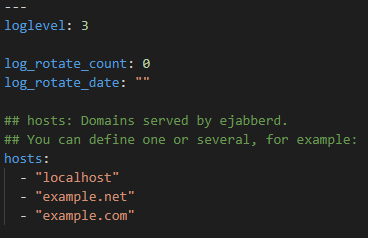
\includegraphics[width=.8\linewidth]{images/exampleYAMLConfig}
  \caption{Formatierung: \texttt{YAML}}
  \label{img:YAMLconfig}
\end{minipage}%
\begin{minipage}{.5\textwidth}
  \centering
  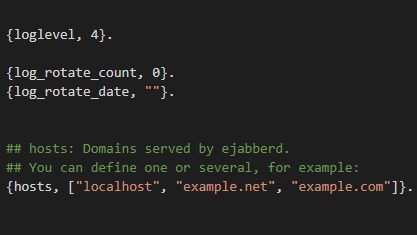
\includegraphics[width=.9\linewidth]{images/ejabberdErlangConfig}
  \caption{Formatierung: \texttt{Erlang}}
  \label{img:ErlangConfig}
\end{minipage}
\end{figure}

Eine genaue Beschreibung der Syntax und dem Aufbau ist in \cite{specificationYAML} vorhanden. \ac{YAML} ist eine vereinfachte Auszeichnungssprache (engl. markup language). Das Ziel des Designs \ac{YAML} ist die Annahme, dass sich jede beliebige Datenstruktur mit assoziativen Listen, Listen (Arrays) und Einzelwerten (Skalaren) darstellen lässt. In \autoref{img:YAMLconfig} beginnt ein in \ac{YAML} formatierter Abschnitt mit drei Bindestrichen. Danach ist beispielhaft ein Skalar \texttt{loglevel} aufgeführt, das wieder auf ein Skalar \texttt{3} abbildet. Diese Syntax entspricht dem Key-Value-Prinzip (Schlüssel-Wert-Prinzip). Die Skalare links vom Doppelpunkt sind Variablen, die auch innerhalb der \ac{YAML}-Datei mit \glqq \texttt{\{ variable \}}\grqq\ referenziert werden können. Werden mehrere Key-Value-Paare Zeile für Zeile aufgelistet, stellt diese Auflistung eine assoziative Liste dar. Das Skalar \texttt{host} ist eine Liste, die mehrere Elemente enthält. Deren Elemente beginnen mit einem Bindestrich. Eine Verschachtelung von Ausdrücken ist durch Einrücken von Ausdrücken möglich. \ac{YAML} erlaubt keine Verwendung von Tabulatoren. Eine Einrückung wird durch eine bestimmte Anzahl an Leerzeichen erzielt. Zeilen mit \texttt{\#} am Anfang sind Kommentare. Durch dieses Konzept ist \ac{YAML} wesentlich leichter von Menschen zu lesen und zu schreiben, außerdem vereinfacht es die Weiterverarbeitung der Daten, da die meisten Sprachen, wie C++, Python oder Java solche Konstrukte bereits integriert haben.

Für das Projekt wird die Konfiguration von ejabberd entsprechend den Empfehlungen aus dem Configuration Guide \cite{ejabberdDoc} in der Auszeichnungssprache \ac{YAML} durchgeführt.

\subsubsection*{Aspekte der Konfiguration}

\begin{itemize}
\item Es werden ausschließlich Clients, die die Kommunikation über das Protokoll \ac{XMPP} unterstützt, wie zum Beispiel Gajim oder Morzilla Thunderbird.

\item Neue Accounts von Benutzern können über In-Band-Registration, das bedeutet, direkt über den \ac{XMPP}-Client eröffnet werden.

\item Es ist grundsätzlich jedem Benutzer gestattet einen Account anzulegen.

\item Aus- und eingehende Kommunikation ist über \ac{TLS} verschlüsselt. Kann der verschlüsselte Kanal nicht aufgebaut werden, zum Beispiel weil der Client die vom Server angebotenen Verschlüsselungsalgorithmen nicht unterstützt, wird die Verbindung abgebrochen.

\item Die Sammlung kryptographischer Verfahren zur Verschlüsselung von Transportdaten (engl. Cipher-Suites) ist im Sinne der Anforderungen aus \autoref{Anforderungen} und des Datenschutzes aus \autoref{chap:Datenschutz} sehr strikt.

\item Die Konfiguration ist nicht für ein Cluster-System oder für die Kopplung von mehreren \ac{XMPP}-Servern vorgesehen.

\end{itemize}

\autoref{tab:PortsEjabberd} zeigt eine Übersicht über alle Standardports und ihrer zugehörigen Dienste.

\begin{table}[h]
\centering
\caption{Übersicht über Ports von ejabberd und deren Dienste}
\begin{tabular}{|l|p{.9\textwidth}|}
\hline
\textbf{Port} & \textbf{Beschreibung} \\
\hline
\textbf{5222} & Clients, die sich über \ac{XMPP} mit dem Server verbinden und kommunizieren wollen, benutzen diesen Port. \\
\hline
\textbf{5223} & \ac{XMPP}-Clients, die sich direkt über \ac{TLS} mit dem Server verbinden wollen, benutzen diesen Port. \\
\hline
\textbf{5269} & Server, die sich mit dem ejabberd-Server verbinden wollen, nutzen diesen Port. \\
\hline
\textbf{5270} & Server, die sich direkt über \ac{TLS} mit dem ejabberd-Server verbinden wollen, benutzen diesen Port.  \\
\hline
\textbf{5280} & Der Zugriff auf das webbasierte Administrationsportal ist unter diesem Port für autorisierte Benutzer möglich. \\
\hline
\end{tabular}
\label{tab:PortsEjabberd}
\end{table}

Die im Folgenden beschriebenen Konfigurationen weichen von der Standardkonfiguration im Auslieferungszustand ab und dienen dem Zweck einer datenschutzfreundlichen und sicheren Konfiguration.

\subsubsection*{Änderung der Datenbank}

Wie in \autoref{sec:Datenbank} beschrieben, ist die interne Mnesia Datenbank nicht für die Verwendung in Produktivumgebungen geeignet und hat nur eine Speicherkapazität von maximal 2 GB. Aus diesem Grund wird die Konfigurationsdatei so angepasst, dass alle Daten in der in \autoref{sec:InstallationEjabberd} installierten MySQL Datenbank gespeichert werden. \autoref{lst:EjabberdDBEinstellung} zeigt die Einstellungen für die Datenbank, die ejabberd verwenden soll.

\begin{lstlisting}[language=yaml, caption={Anpassung der Einstellungen für die Datenbank},label={lst:EjabberdDBEinstellung}]
auth_method: sql
default_db: sql
sql_type: mysql
sql_server: "127.0.0.1"
sql_database: "ejabberd"
sql_username: "ejabberd"
sql_password: "passwort"
sql_port: 3306
\end{lstlisting}

Als Standarddatenbank wird mysql festgelegt. Die Datenbank läuft auf demselben Server wie ejabberd und der Datenbankname ist der des installierten SQL-Schemas, siehe \autoref{sec:InstallationEjabberd}. Hier ist kritisch anzumerken, dass die Zugangsdaten der Datenbank direkt sichtbar in der Konfigurationsdatei hinterlegt sind. Im offiziellen Administration Guide \cite{plainTextConfigSecurity} ist empfohlen, dass nur autorisierte Benutzer ein Lese- und Schreibrecht auf die Konfigurationsdatei bekommen sollen. Dabei stellt sich allerdings die Frage, inwiefern sich das System trotz der eingeschränkten Rechte von Angreifern kompromittieren lässt. Erlangt ein Angreifer die Benutzerdaten eines autorisierten Benutzers hat er uneingeschränkten Zugriff auf sensible Informationen. Wünschenswert wäre eine bessere Möglichkeit, sensible Informationen abzusichern.

\subsubsection*{Konfiguration des Logging}

Das Log-Level bestimmt den Grad der Ausführlichkeit von Einträgen in eine Protokolldatei. Es beeinflusst die Anzahl und den Detailgrad der Informationen, die die Software von ejabberd während dem Betrieb aufzeichnet.\cite{ejabberdDoc}

Verfügbare Log-Level nach \cite{ejabberdDoc}:

\begin{description}
\item[0] Der Server protokolliert alle Aktivitäten, zum Beispiel IP-Adressen von Clients, weitere Informationen zur Verbindung, Fehler und Warnungen.
\item[1] Critical: nur kritische, interne Fehler werden protokolliert. Warnungen und andere Informationen über Benutzer und Verbindungen sind ausgeschlossen.
\item[2] Error: Jeder Fehler wird protokolliert. Andere Informationen über Benutzer oder Verbindungen werden nicht gespeichert.
\item[3] Warning: Alle Warnungen und Fehler werden protokolliert, Verbindungsdetails und Informationen über den Benutzer nicht.
\item[4] Info: Verbindungsdetails und Informationen über den Benutzer werden protokolliert, zusätzlich Warnungen und Fehler jeglicher Art.
\item[5] Debug: Alle Informationen, Fehler und Warnungen werden protokolliert. Detaillierte Informationen über einzelne Module für die Fehlersuche werden erhoben.
\end{description}

Das Log-Level wird auf den Wert \texttt{3} (Warning) gesetzt. Dadurch wird verhindert, das Anmeldevorgänge von Clients oder das Versenden von Nachrichten erfasst wird. Nur Warnungen oder Fehler werden protokolliert.\cite{ejabberdDoc}

\bigskip

\begin{lstlisting}[language=yaml, caption={Einstellung für das Log-Level von ejabberd}]
loglevel: 3
hide_sensitive_log_data: true
\end{lstlisting}

Weil die Option \texttt{hide\_sensitive\_log\_data} aktiviert ist, werden keine IP-Adressen und sensitive Daten protokolliert. Diese Einstellung erhöht die Privatsphäre der Benutzer.\cite{ejabberdDoc}

\subsubsection*{Konfiguration des Host}

Die Liste \texttt{hosts} in \autoref{lst:configHosts} auf Seite \pageref{lst:configHosts} definiert die Domains, deren Benutzer zugeordnet werden können. Eine ejabberd-Instanz kann mehrere Domains verwalten und bedienen. Das Listing zeigt die Konfiguration von ejabberd mit der Domain \texttt{ejabberd-server}. Es ist zulässig, der Liste weitere Domains hinzuzufügen. Für das Projekt wird jedoch nur eine Domain benötigt.

\bigskip

\begin{lstlisting}[language=yaml, caption={Konfiguration der Domains},label={lst:configHosts}]
hosts:
  - "ejabberd-server"
\end{lstlisting}

Die Domain ist gleichzeitig die \ac{XMPP}-Domain mit der Benutzer adressiert werden können. Der Name des Benutzers muss innerhalb der Domain eindeutig sein und mit der vollständigen Domain konkateniert werden, zum Beispiel: \texttt{testuser@ejabberd-server}. Andernfalls ist die Adressierung zum Beispiel für das Versenden und dem Empfang einer Nachricht inkorrekt.


\subsubsection*{Konfiguration der Zertifikate}

Wie Zertifikate für die Verschlüsselung der Transportdaten beantragt werden können, ist in \autoref{sec:InstallationEjabberd} beschrieben. Nach \autoref{lst:ejabberdCerts} befindet sich das Zertifikat und die Datei, die den privaten Schlüssel enthält, im Ornder \texttt{/etc/ejabberd/certs}. Der Ort der Zertifikate muss in der Konfigurationsdatei angegeben werden, sodass ejabberd und ein Client einen verschlüsselten Kanal aufbauen können.

\bigskip

\begin{lstlisting}[language=yaml, caption={Konfiguration der Zertifikate}]
certfiles:
  - "/etc/ejabberd/certs/fullchain.pem"
  - "/etc/ejabberd/certs/xmpp-dhbw.spdns.org.key"
\end{lstlisting}

In der Liste \texttt{certfiles} sind das \ac{RSA}-Zertifikat und die Datei, die den privaten Schlüssel für das Entschlüsseln empfangener Daten beim Aushandeln des Session-Keys beinhaltet, angegeben. Nun kann ein Client das Zertifikat anfordern, mit Hilfe des öffentlichen Schlüssels die Authentizität des Servers überprüfen und den erzeugten Session-Key verschlüsselt übertragen. Der Server entschlüsselt den Session-Key mit seinem privaten Schlüssel aus der \texttt{.key}-Datei.

\subsubsection*{Konfiguration der \ac{TLS}-Parameter}

Der Betreiber von verschlüsselten Diensten muss zwischen Abwärtskompatibilität und Sicherheit abwägen. Beide Aspekte beeinflussen sich gegenseitig. Der Betreiber muss festlegen, ob die Anforderungen an das System ihn dazu zwingen, die Sicherheit des Systems zu reduzieren, sodass Clients, die nur schwächere Verschlüsselungsalgorithmen beherrschen, ebenfalls unterstützt werden. Ist das nicht der Fall, können solche Clients ausgeschlossen und nur noch als sicher eingestufte Algorithmen erlaubt werden, um die Gefährdung der Benutzer zu minimieren.\cite{melzer2010web}

Ein Betreiber eines IT-Service kann sich im offiziellen Wiki des Morzilla Project bei der Wahl der \ac{TLS}-Parameter Unterstützung einholen. Unter \url{https://wiki.mozilla.org/Security/Server_Side_TLS} sind empfohlene Konfigurationen aufgelistet, die nach Kompatibilitätsgrad gruppiert sind.
Die Cipher-Suites, die im Auslieferungszustand vorhanden sind, sind für eine optimale Abwärtskompatibilität zu Clients und zu anderen \ac{XMPP}-Servern ausgelegt und sind nicht sehr strikt. Die Anforderungen aus \autoref{Anforderungen} beinhaltet eine datenschutzfreundliche und sichere Konfiguration. Aus diesem Grund werden nur aktuelle Verschlüsselungsalgorithmen erlaubt und ältere, bereits von der \ac{BSI} als unsicher eingestufte Cipher-Suites werden ausgeschlossen (Stand April 2020).

\bigskip

\begin{lstlisting}[language=yaml, caption={Konfiguration der \ac{TLS} Cipher Suites}, label={lst:ejabberdCipherSuites}]
define_macro:
  'TLS_CIPHERS': "ECDHE-ECDSA-AES256-GCM-SHA384:ECDHE-RSA-AES256-GCM-SHA384:ECDHE-ECDSA-CHACHA20-POLY1305:ECDHE-RSA-CHACHA20-POLY1305:ECDHE-ECDSA-AES128-GCM-SHA256:ECDHE-RSA-AES128-GCM-SHA256:ECDHE-ECDSA-AES256-SHA384:ECDHE-RSA-AES256-SHA384:ECDHE-ECDSA-AES128-SHA256:ECDHE-RSA-AES128-SHA256"
  'TLS_OPTIONS':
    - "no_sslv3"
    - "no_tlsv1"
    - "no_tlsv1_1"
    - "cipher_server_preference"
    - "no_compression"
  'DH_FILE': "/etc/ejabberd/dh4096.pem"

c2s_ciphers: 'TLS_CIPHERS'
s2s_ciphers: 'TLS_CIPHERS'
c2s_protocol_options: 'TLS_OPTIONS'
s2s_protocol_options: 'TLS_OPTIONS'
c2s_dhfile: 'DH_FILE'
s2s_dhfile: 'DH_FILE'
\end{lstlisting}

Um benutzerdefinierte Cipher-Suites für den \ac{TLS}-Verbindungsaufbau zu konfigurieren, werden wie in \autoref{lst:ejabberdCipherSuites} dargestellt, Makros definiert. Das Schlüsselwort \texttt{define\_macro} leitet die Definition von Makros ein. Ein Makro beginnt und endet mit einem Hochkomma, dazwischen wird ein Bezeichner definiert. Dem Makro ist ein Wert zugewiesen. In Zeile 2 des Listings ist das Makro \texttt{TLS\_CIPHERS} definiert, das auf einen Zeichensatz abbildet, der die strikteren Cipher-Suites enthält. So werden nur als sicher eingestufte Verschlüsselungsalgorithmen wie zum Beispiel \ac{AES} mit 128 Bit oder 256 Bit unterstützt. Bereits als unsicher eingestufte Verschlüsselungen wie \ac{DES} werden damit deaktiviert. Das Makro \texttt{TLS\_OPTIONS} definiert die \ac{SSL}-Versionen. Durch den Parameter \texttt{no\_tlsv1\_1} in der Liste, wird ausgeschlossen, dass sich ein Client über ältere \ac{SSL}-Protokollversionen als \ac{TLS}-Version 1.2 mit dem Server verbinden kann. Nur \ac{TLS}-Version 1.2 oder höher werden vom Server unterstützt. Können Server und Client keine Verschlüsselungsalgorithmen oder \ac{TLS}-Versionen vereinbaren, die sie beide unterstützen, lehnt der Server die Verbindung ab. In Zeile 9 ist das Makro \texttt{DH\_FILE} definiert, das auf den absoluten Pfad zur der Datei abbildet, die die erzeugten Diffie-Hellman-Parameter (\autoref{lst:DHParameters}) enthält. In den letzten sechs Zeilen ist aufgezeigt, wie die Makros innerhalb der Konfigurationsdatei referenziert und genutzt werden können. Die benutzerdefinierten Cipher-Suites werden für Verbindungen von Client zu Server (\texttt{c2s\_ciphers}) und Server zu Server (\texttt{s2s\_ciphers} konfiguriert. Zusätzlich werden die benutzerdefinierten Protokollversionen und die Diffie-Hellman-Parameter dem ejabberd-Server zugewiesen. Die Verbindung ist somit mit aktuellen Algorithmen verschlüsselt und Perfect Forward Secrecy (\ac{PFS}) durch die Diffie-Hellman-Parameter vorhanden.

\subsubsection*{Konfiguration der Dienste}

Für die Kommunikation mit Clients oder Servern müssen die Standard-Ports aus \autoref{tab:PortsEjabberd} konfiguriert werden. \autoref{lst:ejabberdPortsConfig} zeigt die Standardkonfiguration, die so ergänzt ist, dass die Änderungen die Sicherheit des Gesamtsystems positiv beeinflussen.

\bigskip

\begin{lstlisting}[language=yaml, caption={Konfiguration der Ports}, label={lst:ejabberdPortsConfig}]
listen:
  -
    port: 5222
    ip: "::"
    module: ejabberd_c2s
    starttls_required: true
    max_stanza_size: 65536
    shaper: c2s_shaper
    access: c2s
  -
    port: 5223
    ip: "::"
    module: ejabberd_c2s
    tls: true
    max_stanza_size: 65536
    shaper: c2s_shaper
    access: c2s
  -
    port: 5269
    ip: "::"
    module: ejabberd_s2s_in
  -
    port: 5270
    ip: "::"
    module: ejabberd_s2s_in
    tls: true
  -
    port: 5280
    ip: "::"
    module: ejabberd_http
    web_admin: true
\end{lstlisting}

\ac{XMPP}-Clients verbinden sich über Port 5222 mit dem Chatserver. Das wird dadurch festgelegt, dass diesem Port das Modul \texttt{ejabberd\_c2s} zugewiesen wird. Der Wert \glqq ::\grqq\ für die IP-Adresse bewirkt, dass der Server auf jeder seiner Netzwerkkarten und IP-Adressen Anfragen akzeptiert. Die Standardkonfiguration wird so ergänzt, dass \texttt{STARTTLS} bei jedem Verbindungsversuch vorausgesetzt wird. Die Option \texttt{max\_stanza\_size} bestimmt die maximale Anzahl an Bytes, die ein \ac{XMPP}-Stanza haben darf. Ist die Anzahl an Bytes über den konfigurierten Wert (65536), wird die Verbindung abgebrochen. In der Standardkonfiguration ist dieser Wert auf \texttt{infinity} gesetzt. Ein Angreifer kann den Server überlasten, wenn er eine hohe Anzahl an sehr großen \ac{XMPP}-Stanzas pro Session sendet. Diese Art des Angriffs bezeichnet man als \ac{DOS}. Die Begrenzung des Wertes vermindert die Wahrscheinlichkeit für den Erfolg eines solchen Angriffs.\cite{XMPPDOS}

Der Port 5223 ergänzt die Standardkonfiguration, sodass sich ein Client direkt via \ac{TLS} verbinden kann. Das bewirkt die Einstellung \texttt{tls: true}, die \texttt{starttls\_required: true} ersetzt.

Für die Verbindung von \ac{XMPP}-Servern zur ejabberd-Instanz ist der Standardport 5269 zuständig. Die Einstellung \texttt{ejabberd\_s2s\_in} bindet diesen Dienst an den Port. Für alle Verbindungen, die durch andere Server initiiert werden, ist \texttt{STARTTLS} notwendig. Das ist in der Standardkonfiguration in einer globalen Einstellung bereits festgelegt. Die globale Einstellung innerhalb der Konfigurationsdatei ist in diesem Listing nicht sichtbar.

Der Port 5270 ergänzt ebenfalls die Standardkonfiguration und dient dazu, dass Server sich direkt via \ac{TLS} mit ejabberd verbinden können.

Der Port 5280 implementiert das Modul \texttt{ejabberd\_http}. Durch die Einstellung \texttt{web\_admin: true} ist das Administrationsportal unter diesem Port verfügbar. Der Administrator dieses Projekts kann sich zum Beispiel unter dieser \ac{URI} in das Webportal einloggen: \texttt{https://xmpp-dhbw.spdns.org:5280/admin}.


\subsubsection*{Konfiguration der Zugriffskontrolle}

Ein Client authentifiziert sich gegenüber dem ejabberd-Server mittels \ac{SASL}. Nach \cite{SASLDescription} ist \ac{SASL} ein Framework, das von verschiedenen Protokollen im Internet für die Authentifizierung verwendet wird. Mittels \ac{SASL} handeln Client und Server standardisiert Authentifizierungsmethoden aus, die von der Applikation transparent genutzt werden.

\pagebreak

Der Betreiber eines ejabberd-Servers sollte für eine sichere Konfiguration veraltete Authentifizierungsmethoden ausschließen (siehe \autoref{lst:excludeOldAuthMechanism}).  

\bigskip

\begin{lstlisting}[language=yaml, caption={Ausschluss unsicherer Authentifizierungsmethoden}, label={lst:excludeOldAuthMechanism}]
disable_sasl_mechanisms:
  - "digest-md5"
  - "x-oauth2"
\end{lstlisting}

Authentifizierungsmethoden die ausgeschlossen werden sollen, werden in die Liste \texttt{disable\_sasl\_mechanisms} eingetragen. Nach \ac{RFC} 6331 ist \texttt{digest-md5} veraltet und unsicher. Er benutzt intern einen \ac{MD5}, den ein Angreifer leicht ermitteln kann und ist empfindlich gegenüber Man-In-The-Middle-Angriffe.\cite{DigestMD5Vulnerabilty}

Auch \texttt{x-oauth2} hat mehrere Sicherheitslücken. Die Methode ist empfindlich gegenüber \ac{DOS}-Angriffe. Nach \cite{xOAuthVulnerabilty} kann ein nicht authentifizierter Angreifer, den Server überlasten.

In \autoref{lst:AddAdminUserEjabberd} auf Seite \pageref{lst:AddAdminUserEjabberd} ist beschrieben, wie ein Benutzer mit administrativen Rechten auf dem Server angelegt werden kann. In der Standardkonfiguration ist der Benutzer \glqq admin\grqq\ berechtigt auf das Administrationsportal mit der Domain \texttt{localhost} zuzugreifen. Damit der Benutzer berechtigt ist, auf die für das Projekt erstellte Domain \texttt{ejabberd-server} zuzugreifen, muss die \ac{ACL} angepasst werden. Hierfür trägt ändert man im Abschnitt \texttt{acl} der Konfigurationsdatei die Domain, auf die der Benutzer \glqq admin\grqq\ verweist. Das Ergebnis der Änderung ist in \autoref{lst:aclChangeAdmin} dargestellt.

\bigskip

\begin{lstlisting}[language=yaml, caption={Anpassung der Access Control List (ACL) für den administrativen Zugriff},label={lst:aclChangeAdmin}]
acl:
  admin:
     user:
       - "admin": "ejabberd-server"
\end{lstlisting}


Nach all den durchgeführten Änderungen muss der Server mit dem Kommando \texttt{sudo systemctl restart ejabberd} neu gestartet werden.

\pagebreak

\subsubsection*{Überblick über das Administrationsportal}

Der Administrator kann sich mit Benutzername und Passwort in das Webportal einloggen. \autoref{img:AdminPortalEjabberdOverview} zeigt im linken Bild das Webportal nach einem Login.

\begin{figure}[h]
\centering
\begin{minipage}{.5\textwidth}
  \centering
  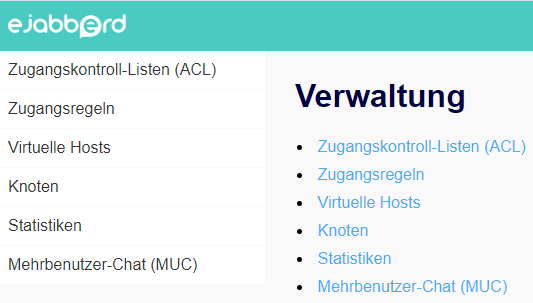
\includegraphics[width=.9\linewidth]{images/AdminPortalEjabberdOverview}
\end{minipage}%
\begin{minipage}{.5\textwidth}
  \centering
  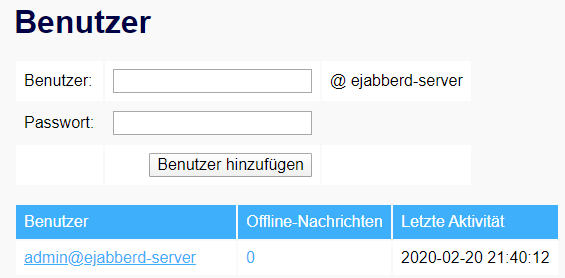
\includegraphics[width=\linewidth]{images/AdminPortalAddUsers}
\end{minipage}
\caption{Links Übersicht: Administrationsportal, rechts: Übersicht: Benutzerverwaltung, eigene Darstellung}
\label{img:AdminPortalEjabberdOverview}
\end{figure}

Mit einem Klick auf \texttt{Virtuelle Hosts} sieht man alle Domains, die auf dem ejabberd-Server registriert sind. Für dieses Projekt sieht man in der Übersicht die Domain \texttt{ejabberd-server} und die Anzahl der vorhandenen und aktuell angemeldeten Benutzer. Klickt man auf eine Domain und dann in der Auswahl auf \texttt{Benutzer}, können Benutzer verwaltet werden, siehe \autoref{img:AdminPortalEjabberdOverview} rechte Abbildung.

\subsubsection*{Konfiguration weiterer Module}

Welche weiteren Möglichkeiten es gibt, die Konfiguration von ejabberd sicherer und datenschutzfreundlicher zu machen, zeigt dieser Abschnitt auf.

Mit Shaper-Rules lassen sich unter anderem die maximale Anzahl an Verbindungen (Sessions) pro Benutzer einschränken.  

\bigskip

\begin{lstlisting}[language=yaml, caption={Anpassung der Shaper-Rules}]
shaper_rules:
  max_user_sessions: 10
  max_user_offline_messages:
    - 5000: admin
    - 500
\end{lstlisting}

Wie im Listing dargestellt, werden die Anzahl an Sessions pro Benutzer auf zehn verringert, um eine Überlastung des Servers und damit einen Systemausfall vorzubeugen. Zusätzlich wird die maximale Anzahl an Nachrichten, die der Server speichert, bis der Benutzer erneut online ist auf 500 reduziert. Diese Art von Nachrichten werden als Offline-Nachrichten bezeichnet. Die Anzahl an Offline-Nachrichten für den Benutzer \glqq admin\grqq\ mit 5000 Nachrichten ist vorkonfiguriert.

Ein weiteres wichtiges Modul ist \texttt{mod\_disco}. Dieses Modul erlaubt es, einem Client Kontaktinformationen zu zustellen, damit ein Benutzer Spam oder Missbrauch melden kann.

\bigskip

\begin{lstlisting}[language=yaml, caption={Kontaktinformationen für Spam- oder Missbrauchsmeldungen}]
mod_disco:
  server_info:
    -
      modules: all
      name: "abuse-addresses"
      urls:
        - "mailto:admin@mail.de"
    -
      modules: all
      name: "support-addresses"
      urls:
        - "mailto:admin@mail.de"
\end{lstlisting}

Das Listing zeigt wie in der Liste \texttt{server\_info} zusätzliche Informationen über den Server hinterlegt werden können. Ejabberd ünterstützt die \ac{XMPP}-Erweiterung \texttt{XEP-0157: Contact Addresses for XMPP Services}. Der Client sendet eine Anforderung über \ac{XMPP}. Der Server sendet dem Client die Kontaktinformationen zu. Der Client präsentiert dem Benutzer die Ergebnisse. Der genaue Ablauf ist in  \cite{xepContactInformation} beschrieben. Der Wert \texttt{all} bei \texttt{modules} bewirkt, dass die für alle Module, die ejabberd dem Client zur Verfügung steht, die Kontaktinformationen zugeordnet ist. Alternativ lässt sich eine Liste von bestimmten Modulen übergeben. Die Kontaktinformation ist dann nur für die in der Liste angegebenen Modulen abrufbar. Über den \texttt{url} Parameter lassen sich E-Mail Adressen oder bestimmte \ac{URI}s angeben.

Das Modul \texttt{mod\_last} protokolliert den Zeitpunkt, zu dem sich ein Client am System an- oder abmeldet. Im Sinne einer datenschutzfreundlichen Konfiguration wird das Modul durch Auskommentieren in der Konfigurationsdatei deaktiviert.

Nach den Anforderungen aus \autoref{Anforderungen} ist eine Nachrichtenarchivierung erforderlich. Eine Nachrichtenarchivierung ist eine gängige Funktionalität, die ein \acs{IMS} dem Benutzer bereitstellt. Deshalb ist eine Speicherung des Nachrichtenverlaufs notwendig. Zudem gibt es Clients, deren interner Speicherplatz zu gering ist, um Nachrichten selbst persistent zu speichern. Aus diesen Gründen kann das Modul \ac{MAM} aktiviert werden. Es ist in der \ac{XMPP}-Erweiterung \texttt{XEP-0313} spezifiziert.\cite{xepMAM}

Wichtige Funktionen von \ac{MAM} nach \cite{xepMAM}:

\begin{itemize}
\item Archivierung von Nachrichten auf dem Server
\item Archivierung der Nachrichten eines Multi-User-Chats (Gruppen-Chat)
\item Abruf der Nachrichten durch ein \ac{XMPP}-Query Request durch Clients
\item Synchronisation des Nachrichtenverlaufs zwischen mehreren Clients
\end{itemize}

\texttt{XEP-0313} spezifiziert viele weitere Funktionen, für die \ac{MAM} eingesetzt werden kann. In diesem Projekt wird jedoch nur die erste Funktion implementiert. Nach \cite{xepMAM} muss ein \ac{XMPP}-Server \ac{MAM} nicht zwingend bereitstellen und die Kontrolle über die Einstellungen kann der Betreiber des Servers festlegen. Das Protokoll erlaubt einem Benutzer aber auch, die Einstellungen für die Nachrichtenarchivierung selbst festzulegen, sodass dieser entscheiden kann, ob er Nachrichten auf dem Server archivieren möchte oder nicht. Ein Client, der diese XEP-Erweiterung unterstützt, informiert den Server über die Änderungen in den Einstellungen oder kann die aktuellen Einstellungen vom Server abfragen.\cite{xepMAM}

\autoref{img:MAMGetRequest} zeigt typische Kommunikationsverläufe.

\begin{figure}[h]
\centering
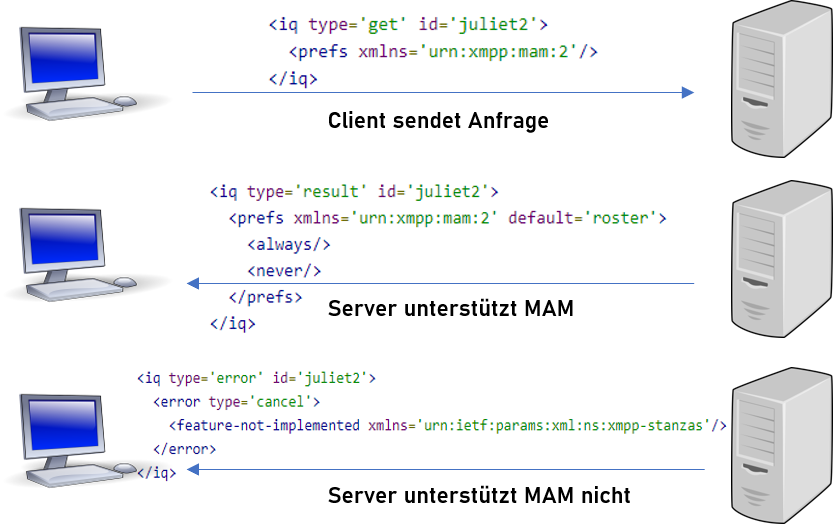
\includegraphics[width=.7\linewidth]{images/XEP0313_GetRequest}
\caption{Anfrage des Client zum Abruf der aktuellen \ac{MAM} Einstellungen \cite{xepMAM}, eigene Darstellung}
\label{img:MAMGetRequest}
\end{figure}

Der Client sendet eine Anfrage vom Typ \texttt{get} mit seiner Benutzer-ID. Im Element \texttt{prefs} gibt er das Protokoll \ac{MAM} an. Darunter sind zwei mögliche Antworten des Servers abgebildet. Im ersten Fall unterstützt der Server \ac{MAM} und antwortet mit den aktuellen Einstellungen des Benutzers. Das \texttt{prefs}-Element muss vorhanden sein. Dieses enthält die konfigurierten Richtlinien für die Archivierung. Die Elemente \texttt{always} und \texttt{never} müssen immer im \texttt{prefs}-Element enthalten sein, auch wenn sie leer sind. Sie beinhalten eine Liste von \texttt{jid}-Elemente (Jabber-IDs). Für die Jabber-IDs im Element \texttt{always} ist die Archivierung immer aktiv. Für die IDs im Element \texttt{never} archiviert der Server niemals Nachrichtenverläufe. Im dritten Teilbild ist eine alternative Antwort des Servers an den Client dargestellt. Der Server antwortet mit einer \ac{XMPP}-Nachricht vom Typ \texttt{error} und dem Element \texttt{feature-not-implemented}, wenn er \ac{MAM} nicht unterstützt oder die Funktion deaktiviert ist.\cite{xepMAM}

Der Autor Wild \cite{xepMAM} beschreibt, dass die Einstellungen der Archivierung mit einer Anfrage vom Typ \texttt{set} auch verändert werden können. Die Anfrage ist in \autoref{img:MAMUpdate} gezeigt.

\begin{figure}[h]
\centering
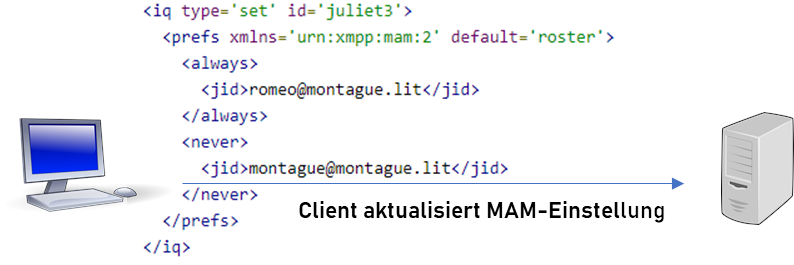
\includegraphics[width=.8\linewidth]{images/XEP0313_UpdateRequest}
\caption{Aktualisierung der Archivierungseinstellungen durch den Client \cite{xepMAM}, eigene Darstellung}
\label{img:MAMUpdate}
\end{figure}

Der Server speichert die Einstellungen nach Erhalt der Anfrage. Er archiviert von diesem Zeitpunkt an alle Nachrichten für die Jabber-ID \texttt{romeo@montague.lit}. Für den Benutzer der ID \texttt{montague@montague.lit} werden keine Nachrichten mehr in der Datenbank gespeichert.

\autoref{lst:sqlSettingsEjabberd} zeigt die Einstellungen von ejabberd für \ac{MAM}, die für dieses Projekt konfiguriert sind.

\bigskip

\begin{lstlisting}[language=yaml, caption={Konfiguration der Einstellungen für die Nachrichtenarchivierung}, label={lst:sqlSettingsEjabberd}]
mod_mam:
    db_type: sql
    assume_mam_usage: true
    default: always
    request_activates_archiving: true
\end{lstlisting}


Das Modul \texttt{mod\_mam} realisiert die zuvor beschrieben Funktionen von \ac{MAM}. Einerseits schreibt der Datenschutz vor, dass der Benutzer Kontrolle über seine Daten behalten muss, andererseits sind Nachrichtenverläufe hilfreich für Benutzer, um den Kontext der Nachrichten zu verstehen. Aus diesem Grund ist ein Kompromiss in der Einstellung festzulegen. Die Nachrichten sollen nur archiviert werden, wenn ein Benutzer das ausdrücklich veranlasst. Durch der aktivierten Einstellung \texttt{request\_activates\_archiving} speichert ejabberd nur dann Nachrichten, wenn der Client eine Anfrage sendet, die diese Archivierung aktiviert. Sendet ein Client diese Anfrage, werden ab diesem Zeitpunkt an alle Nachrichten des Client gespeichert. Mit \texttt{db\_type: sql} wird festgelegt, dass die Nachrichten in der in \autoref{sec:InstallationEjabberd} installierten MySQL Datenbank gespeichert werden.

Über das Modul \texttt{mod\_roster} kann vermieden werden, dass bei jedem Login die gesamte Kontaktliste (Roster) eines Benutzers erneut heruntergeladen werden muss. Das folgende Listing zeigt die Einstellungen.

\bigskip

\begin{lstlisting}[language=yaml, caption={Einstellungen des Moduls mod\_rosters}]
mod_roster:
  versioning: true
\end{lstlisting}

Dadurch wird die \ac{XMPP}-Erweiterung \texttt{XEP-0237: Roster Versioning} \cite{xep0237RosterVersioning} aktiviert und sorgt dafür, dass die Kontaktliste nur bei Änderungen erneut heruntergeladen werden muss. Das Verfahren spart damit Bandbreite ein.

Abschließend werden aus Sicherheitsgründen das Modul \texttt{mod\_version} und \texttt{mod\_http\_api} angepasst. Die Anpassungen sind in \autoref{lst:ejabberdImportantSecuritySettings} dargestellt.

\begin{lstlisting}[language=yaml, caption={Konfiguration relevanter Module für die Sicherheit von ejabberd},label={lst:ejabberdImportantSecuritySettings}]
mod_version: 
  show_os: false

## mod_http_api: {}
\end{lstlisting}

Ein Client kann die Version des Betriebssystems, auf dem ejabberd installiert ist, grundsätzlich abfragen. Das wird durch die Einstellung \texttt{show\_os: false} verhindert. Ebenfalls wird das Modul \texttt{mod\_http\_api} deaktiviert. Eine Administration über das \ac{HTTP} ist damit nicht möglich. Die ejabberd-Instanz kann nur noch über das erlang Kommandozeilenprogramm \texttt{ejabberdctl} verwaltet werden, siehe \autoref{lst:AddAdminUserEjabberd}.

Nun ist ejabberd für den Gebrauch in der Projektarbeit konfiguriert. Der Server kann nun von jedem beliebigen \ac{XMPP}-Client genutzt werden.

\pagebreak

\chapter{Apache Kafka für moderne Echtzeitübertragung}
\label{chap:KafkaDescription}

Warum es sinnvoll ist für die Umsetzung eines \acs{IMS}, Messaging-Systeme wie Apache Kafka einzusetzen, ist in \autoref{chap:VerprbungIMS} ausführlich erörtert. Dieses Kapitel beschreibt die Funktionsweise von Apache Kafka. 

Apache Kafka ist eine verteilte Event-Streaming-Plattform \cite{kafkaConfluent}. Konkret bezeichnet Nannoni in seiner Dissertation \cite{nannoniDissKafka} Kafka als eine Message Broker\footnote{Message Broker: Einrichtung zur Vermittlung von Nachrichten zwischen einem Sender und einem oder mehreren Empfängern, siehe \autoref{chap:VerprbungIMS}.} Middleware\footnote{Software, die die Anwendungsschicht unabhängig vom Betriebssystem von den darunterliegenden Schichten entkoppelt.}. Die Plattform ist seit 2011 ein Apache Incubator\footnote{Projekt der \ac{ASF} um sicherzustellen, dass die geförderte Software frei von rechtlichen Konflikten und kompatibel mit den Leitprinzipien der Open-Source-Stiftung ist.\cite{asfIncubator}} und wird seit 2012 von der Apache Software Foundation entwickelt und gepflegt\cite{kafkaConfluent}. \autoref{img:kafkaMainArchitecture} zeigt die globale Architektur von Apache Kafka.

\begin{figure}[h]
	\centering
	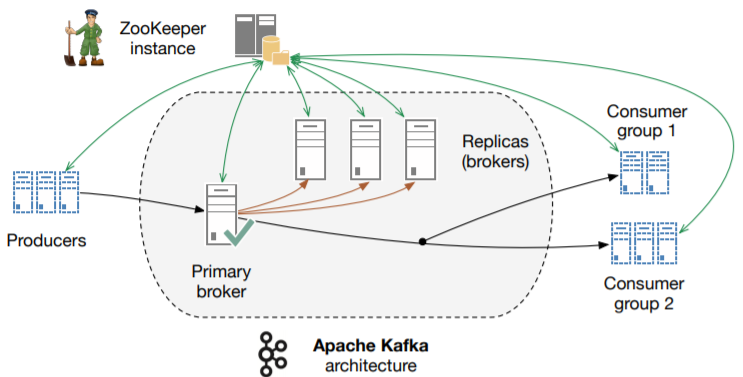
\includegraphics[width=\textwidth]{images/kafkaMainArchitecture}
	\caption{Globale Architektur von Apache Kafka mit einem Topic, einer Partition und Replikationsfaktor 4 \cite{nannoniDissKafka}}
	\label{img:kafkaMainArchitecture}
\end{figure}

Die Architektur von Apache Kafka besteht aus Topics, Producers, Consumers, und Brokers. Alle Nachrichten befinden sich in Partitionen, die wiederum in den Brokern liegen.
Um eine Nachricht zu lesen oder zu schicken, muss immer das jeweilige Topic einer Partition angegeben werden.
Apache Kafka speichert die Partitionen (inklusive Nachrichten) auf den Brokern in einem eigenen, binären Dateiformat. Die Plattform kann aus einem einzigen Kafka Broker oder, wie \autoref{img:kafkaMainArchitecture} zeigt, aus mehreren Kafka Brokern bestehen. Es muss aber immer ein Primary Broker vorhanden sein, der die Nachrichten speichert und je nach Konfiguration auf weiteren Brokern repliziert, um die Ausfallsicherheit und Verfügbarkeit zu erhöhen. In der \autoref{img:kafkaMainArchitecture} sind vier Kafka Broker abgebildet, weshalb der Replikationsfaktor (englisch Replication factor) gleich 4 ist. Entsprechend der offiziellen Dokumentation bietet diese Persistence-By-Design Architektur die maximale Sicherheitsstufe gegen Software-Abstürze ohne, dass das System an Leistung verliert. Diese Skalierbarkeit ist in Kafka so tief verankert, dass ein nicht-repliziertes Kafka-System aus technischer Sicht lediglich ein Kafka-System mit dem Replikationsfaktor 1 ist. Ein Kafka Broker funktioniert nicht ohne eine externe Apache Zookeeper Instanz. Zookeeper ist für die Koordination zwischen Producer, Apache Kafka und Consumer zuständig. Zusätzlich bietet dieser das verteilte Konfigurieren und Synchronisieren, sowie ein Namensregister für die einzelnen Broker des verteilten Systems an.\cite{nannoniDissKafka}

Berle ist der Auffassung, dass das Funktionsspektrum von Kafka hinter dem eines \ac{IMS} liegt, aber Kafka durch seine Vielseitigkeit und dem hohen Datendurchsatz oft anderen vergleichbaren Systemen überlegen ist \cite{berleKafkaOverview}. Vergleichbare Systeme wie RabbitMQ oder HornetQ sind für geringe Datenmengen schneller, für große Datenmengen hat Apache Kafka aber einen höheren Datendurchsatz. Der Unterschied des Datendurchsatzes wird an Hand der \autoref{tab:performanceKafka} mit den Messergebnissen von Quadri deutlich \cite{quardriKafkaPerformance}.

\begin{table}[h]
\centering
\caption{Vergleich des Datendurchsatzes bei Versenden und Empfangen von Nachrichten von Apache Kafka mit anderen Technologien}
\begin{tabular}{|l|r|r|}
\hline
\textbf{Technologie} & \textbf{Senden (Nachrichten/s)} & \textbf{Empfangen (Nachrichten/s)} \\
\hline
\texttt{Apache Kafka} & 33000 & 31000 \\
\hline
HornetQ & 17000 & 16000 \\
\hline
SQS-1node & 14000 & 4000\\
\hline
RabbitMQ-batch100 & 3000 & 3000 \\
\hline
\end{tabular}
\label{tab:performanceKafka}
\end{table}

Estrada und Ruiz definieren Apache Kafka wie folgt:
\glqq Apache Kafka is a real-time publish-subscribe solution messaging system: open source, distributed, partitioned, replicated, commit-log based with a publish-subscribe schema.\grqq\footnote{\cite[S.166]{estradaRuiz2016}}

Die Definition lässt sich wie folgt interpretieren und die Arbeitsweise daraus ableiten:
Apache Kafka ist ein verteiltes persistentes Log, das als ereignisorientiertes (englisch Publish/Subscribe) Messaging System genutzt werden kann. In diesem verteilten Log werden Nachrichten als Key-Value-Paar gespeichert. Nach Tanenbaum \cite{andrew2008verteilte} ist die grundlegende Idee von ereignisorientierten Architekturen, dass Prozesse Ereignisse veröffentlichen (publish) und nur die Prozesse diese Ereignisse empfangen, die sie abonniert (subscribe) haben. Hinzu kommt, dass Kafka die Nachrichten von Ereignissen persistent speichern kann, weshalb Kafka in die Architekturen von verteilten Systemen als Hybrid eingeordnet werden kann, siehe \autoref{img:PublishSubscribeTanenbaum}.

\begin{figure}[h]
	\centering
	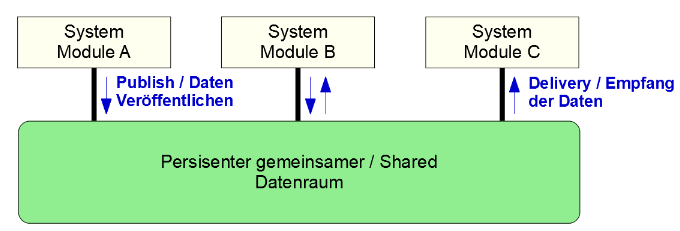
\includegraphics[width=.8\textwidth]{images/PublishSubscribeTanenbaum}
	\caption{Hypride Architektur eines ereignisorientierten Systems mit persistentem Datenspeicher \cite{richterArchitekturVS}}
	\label{img:PublishSubscribeTanenbaum}
\end{figure}

Die einzelnen Systeme werden durch diesen Ansatz zeitlich entkoppelt. Modul C muss nicht aktiv sein, wenn Modul A eine Nachricht veröffentlicht. Der persistente Datenraum speichert die Nachricht, sodass Modul C diese abholen kann, wenn es wieder aktiviert wird. Diese Funktion übernehmen klassisch spezialisierte \ac{MQ} Systeme, wie beispielsweise RabbitMQ, ActiveMQ und viele weitere. Die Hauptunterschiede liegen in der horizontalen Skalierbarkeit für große Datenmengen. Beispielsweise betreibt Microsoft Oracle ein Kafka Cluster mit 1300 Brokern, der 1 Trillion Nachrichten pro Tag verarbeitet \cite{ritchieKafkaMicrosoft}. Die Kafka Plattform ist skalierbar und kann durch viele zusätzliche Kafka Broker erweitert werden. Sie verbindet heterogene Clients miteinander, in dem sie den Clients die Kommunikation untereinander ermöglicht.

\pagebreak

Konkret ist die ereignisorientierte Architektur in Apache Kafka wie folgt umgesetzt, siehe \autoref{img:kafkaPrinciple}:

\begin{figure}[h]
	\centering
	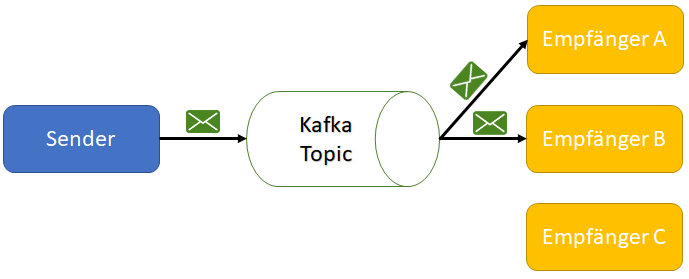
\includegraphics[width=.8\textwidth]{images/principleKafka}
	\caption{Funktion des Publish/Subscribe Prinzips von Apache Kafka, eigene Darstellung}
	\label{img:kafkaPrinciple}
\end{figure}

Ein Sender (englisch Producer) produziert Nachrichten in ein Topic. Dieser Vorgang entspricht einer Publish Aktion der ereignisorientierten Architektur. Empfänger (englisch Consumer) konsumieren die Nachrichten aus diesem Topic, was der Subscribe Aktion entspricht. Die Nachricht, auch Record genannt, stellt dabei das Ereignis dar und wird erst bei Bedarf aus dem Topic gelöscht. Ein Topic in Kafka ist nach Berle \cite{berleKafkaOverview} eine logische Instanz, zu der Nachrichten gesendet und ausgelesen werden können. Je nach Konfiguration besteht ein Topic aus einer endlichen Anzahl N an Partitionen. Ein Kafka Broker ist verantwortlich für mehrere Topics und deren N Partitionen. \autoref{img:kafkaTopicExample} zeigt die Architektur eines Topics.

\begin{figure}[h]
	\centering
	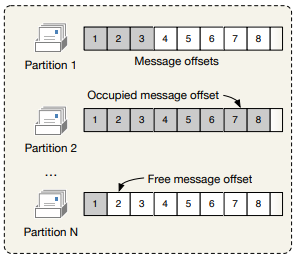
\includegraphics[width=.55\textwidth]{images/kafkaTopicExample}
	\caption{Architektur eines Topics \cite{nannoniDissKafka}}
	\label{img:kafkaTopicExample}
\end{figure}

Ein Producer entscheidet selbst, in welche Partitionen er welche Datensätze schreibt \cite{berleKafkaOverview}. In einigen Anwendungsfällen kann das relevant sein, typisch wird jedoch ein Round-Robin-Verfahren gewählt, bei dem nach einer bestimmten Anzahl an Nachrichten die Partitionen abwechselnd verwendet werden \cite{berleKafkaOverview}. \autoref{img:kafkaTopicExample} zeigt, dass innerhalb eines Topics die Nachrichten ungleichmäßig auf Partitionen verteilt sein können.

Eine Nachricht ist mit einem Offset gekennzeichnet \cite{berleKafkaOverview, nannoniDissKafka}. Der Offset ist innerhalb einer Partition eine eindeutige Ganzzahl. Bei jedem Eintreffen einer Nachricht wird der Offset inkrementiert. Trifft in \autoref{img:kafkaTopicExample} eine Nachricht in die Partition 1 wird ihr der Offset 4 zugeordnet, trifft sie in Partition N erhält die Nachricht den Offset 2. Durch dieses Konzept empfangen Consumer die Nachrichten in der Reihenfolge, in der sie ein Producer versendet. Die eindeutige Kennzeichnung ermöglicht es Consumern, auch vergangene Nachrichten ab einem bestimmten Offset zu konsumieren.\cite{nannoniDissKafka}

Kafka speichert die Nachrichten immer auf der Festplatte. Die Nachrichten müssen irgendwann mit einer der folgenden Richtlinien (Cleanup Policies) \cite{berleKafkaOverview} gelöscht werden, weil die Festplattenauslastung ansonsten zu groß wird:

\begin{description}
\item[Retention-Time:] Die ältesten Daten werden frühestens nach einer frei definierbaren Zeit gelöscht. In der Standardeinstellung ist diese Zeit mit 7 Tagen definiert.
\item[Retention-Size:] Die ältesten Daten werden frühestens gelöscht, sobald der Speicherbedarf der Nachrichten eine definierte Größe erreicht hat.
\item[Log-Compaction:] Es werden nur Nachrichten aus dem Log gelöscht, deren Schlüssel mehrfach vorkommt und niemals die neueste Nachricht mit dem Schlüssel. Für mehr Informationen, siehe \cite{kafkaLogCompaction}.
\end{description}

Die Standardeinstellung ist die Retention-Time.

\pagebreak

\subsubsection*{Consumer Gruppen}

Aus einem Topic kann eine Nachricht solange wiederholt gelesen werden, bis die Cleanup Policy die Nachrichten löscht. Durch Consumer Gruppen kann ein Kafka Broker sich auch als Queue verhalten \cite{nannoniDissKafka}. Die Funktionsweise von Consumer Gruppen verdeutlicht \autoref{img:kafkaConsumerGroups}.

\begin{figure}[h]
	\centering
	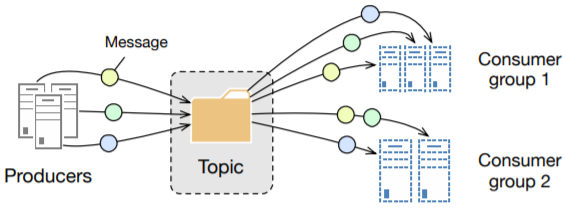
\includegraphics[width=.8\textwidth]{images/kafkaConsumerGroups}
	\caption{Konzept der Consumer Gruppe: Beispiel mit einem Topic und einer Partition \cite{nannoniDissKafka}}
	\label{img:kafkaConsumerGroups}
\end{figure}

Jeder Consumer kann zu einer Consumer Gruppe gehören. Eine Consumer Gruppe kann jede Nachricht eines Kafka Topics nur einmal lesen. Angenommen zwei Consumer sind dergleichen Consumer Gruppe zugeordnet. Lesen beide aus dem gleichem Topic, lesen beide niemals die gleiche Nachricht, sondern verschiedene. Konsumieren zwei Consumer Gruppen aus dem gleichen Topic, erhalten beide Consumer Gruppen eine Kopie der Nachrichten. Innerhalb der Consumer Gruppe kann eine Nachricht jedoch nur einmal gelesen werden.\cite{berleKafkaOverview, nannoniDissKafka}

\textbf{Bemerkung:} Berle \cite{berleKafkaOverview} betont, dass in der Praxis häufig einer gesamten Applikation eine Consumer Gruppe zugeordnet werden. Consumer sind Threads, die aus derselben Consumer Gruppe konsumieren, um die Nachrichten schneller konsumieren zu können.

\pagebreak

\section{Installation von Apache Kafka}
\label{sec:InstallationKafka}

Die nachfolgende Anleitung bezieht sich auf die Installation eines Kafka-Systems. Die Installationsanleitung beschreibt alle notwendigen Schritte, um einen Server mit der Kafka Version 2.4.0 in Betrieb zu nehmen. Die Anleitung beschreibt nicht, wie ein Cluster-System, welches einen Verbund mehrerer Kafka Broker darstellt, in Betrieb genommen werden kann. Ziel ist es, eine einfache Installation aufzuzeigen und Kafka als Service auf einem Server bereitzustellen ohne, dass für die Ausführung der Kafka-Instanz ein Benutzer angemeldet sein muss. Die Informationen und Befehle sind aus der Kafka-Dokumentation \cite{kafkaDoc} zu entnehmen.

\bigskip

\textbf{Voraussetzungen:}

\smallskip

\begin{itemize}
\item Linux Ubuntu 18.04 LTS
\item Server
\begin{itemize}
\item mindestens 4GB RAM, empfohlen 8GB (Installation mit weniger RAM kann zu Problemen beim Start von Kafka führen, weil die Java Virutal Machine (JVM) eine \glqq OutOfMemory\grqq\ -Exception werfen kann.
\end{itemize}
\item OpenJDK 8 (Kafka ist in der Programmiersprache Java programmiert und benötigt deshalb eine lauffähige JVM.)
\end{itemize}

\subsubsection*{Anlegen eines Benutzers}

Für die Erstellung eines Benutzers muss sich auf dem Server mit einem Benutzer eingeloggt werden. Mit folgendem Kommando wird ein Benutzer mit dem Namen Kafka angelegt. Mit dem zweiten Kommando wird der Benutzer der \glqq sudo\grqq\ -Gruppe hinzugefügt und ist ab diesem Zeitpunkt berechtigt höher privilegierte Befehle auszuführen. Das letzte Kommando legt ein Passwort an, dass bei der Ausführung höher privilegierter Befehle abgefragt wird.

\smallskip

\begin{lstlisting}[language=Bash]
$ sudo adduser kafka # Benutzer anlegen
$ sudo adduser kafka sudo # Benutzer zur sudo-Gruppe hinzufügen
$ sudo passwd kafka # Anlegen eines sudo-Passwords
\end{lstlisting}

Anschließend muss sich mit dem neu erstellten Benutzer eingeloggt werden (Kommando: su kafka).

\subsubsection*{Installation der benötigten Komponenten}


Als nächstes muss das komprimmierte Kafka-Binary heruntergeladen werden. Hierzu kann das \texttt{curl}-Kommandozeilentool verwendet werden, um das Binary direkt aus dem Internet herunterzuladen und im Home-Verzeichnis des kafka-Benutzers gespeichert werden.

\smallskip

\begin{lstlisting}[language=Bash]
$ curl "http://mirror.checkdomain.de/apache/kafka/2.4.0/kafka_2.12-2.4.0.tgz" -o ~/kafka_2.12-2.4.0.tgz
\end{lstlisting}

Falls OpenJDK 8 noch nicht installiert ist, muss folgender Befehl ausgeführt werden.

\smallskip

\begin{lstlisting}[language=Bash]
$ sudo apt-get install openjdk-8-jdk
\end{lstlisting}

Erstellen Sie ein Grundverzeichnis in dem alle Kafka-Komponenten extrahiert werden können. Legen Sie mit folgendem Befehl ein Verzeichnis mit dem Namen \glqq kafka\grqq\ an. Extrahieren Sie die komprimierte Datei in dasselbe Verzeichnis.

\smallskip

\begin{lstlisting}[language=Bash]
$ mkdir ~/kafka && cd ~/kafka
$ tar -xvzf ~/kafka_2.12-2.4.0.tgz --strip 1
\end{lstlisting}

Kafka ist ab jetzt bereit für eine Konfiguration.

\subsubsection*{Konfiguration von Kafka}

Kafka lässt es in der Standardkonfiguration nicht zu neue Topics, eine Kategorie oder eine Gruppe zu löschen. Um das zu ändern, muss die Konfigurationsdatei von Kafka angepasst werden. Falls der \glqq nano\grqq\ -Editor auf Ihrem System nicht verfügbar ist, können Sie einen Editor Ihrer Wahl verwenden, zum Beispiel \glqq vi\grqq.

\smallskip

\begin{lstlisting}[language=Bash]
$ nano ~/kafka/config/server.properties
\end{lstlisting}

Fügen Sie diese Einstellung in der Datei hinzu:

\texttt{delete.topic.enable = true}

Speichern Sie anschließend die Datei und beenden Sie den Editor.

Kafka benötigt Zookeeper, um starten zu können. Zookeeper ist automatisch nach der Installation aus Schritt 2 vollständig vorhanden und befindet sich ebenfalls im erstellten \glqq kafka\grqq\ -Verzeichnis. Testen Sie mit folgenden Kommandos, ob Zookeeper und Kafka erfolgreich starten. Starten Sie zuerst Zookeeper, warten Sie 30 Sekunden, öffnen Sie eine zweite CLI auf dem System und starten Sie anschließend Kafka. Wird kein Fehler geworfen, waren alle Schritte bisher erfolgreich verlaufen und Kafka ist betriebsbereit.

\smallskip

\begin{lstlisting}[language=Bash]
$ ~/kafka/bin/zookeeper-server-start.sh ~/kafka/config/zookeep.properties # Start: zookeeper
$ ~/kafka/bin/kafka-server-start.sh ~/kafka/config/server.properties # Start: kafka
\end{lstlisting}

Zeigt der Kommandozeilen-Output nur Nachrichten der Kategorie \glqq INFO\grqq\ und keine Fehlermeldungen, sind beide Dienste erfolgreich gestartet. Ansonsten überprüfen Sie Ihre Schritte erneut und korrigieren Sie die Fehler.

Für den Start von Kafka ist im aktuellen Zustand eine Anmeldung des Benutzers erforderlich, der Zookeeper und Kafka als Benutzerprozess startet. Um Kafka als Server-Dienst bereitzustellen folgen Sie dem nächsten Kapitel der Anleitung. Möchten Sie lediglich die Grundfunktionalitäten ausprobieren und benötigen keine globale Verfügbarkeit, kann Schritt 4 der Anleitung entfallen.

\subsubsection*{Bereitstellung von Kafka als Dienst auf einem Server}

Teilschritte für die Bereitstellung als Server-Dienst:

\begin{itemize}
\item Systemd-Datei für Zookeeper erstellen
\item Systemd-Datei für Kafka erstellen
\item Zookeeper-Dienst starten
\item Kafka-Dienst starten
\end{itemize}

\bigskip

\textbf{Systemd-Datei für Zookeeper erstellen:}

\bigskip

\begin{lstlisting}[language=Bash]
$ sudo nano /etc/systemd/system/zookeeper.service
\end{lstlisting}

Folgender Inhalt muss in die Datei kopiert werden:

\smallskip

\begin{lstlisting}[language=Bash]
[Unit]
Requires=network.target remote-fs.target
After=network.target remote-fs.target

[Service]
Type=simple
User=kafka
ExecStart=/home/kafka/kafka/bin/zookeeper-server-start.sh /home/kafka/kafka/config/zookeeper.properties
ExecStop=/home/kafka/kafka/bin/zookeeper-server-stop.sh
Restart=on-abnormal

[Install]
WantedBy=multi-user.target
\end{lstlisting}

Speichern Sie die Datei und gehen Sie zum nächsten Schritt.

\textbf{Systemd-Datei für Kafka erstellen:}

\bigskip

\begin{lstlisting}[language=Bash]
$ sudo nano /etc/systemd/system/kafka.service
\end{lstlisting}

Folgender Inhalt muss in die Datei kopiert werden:

\smallskip

\begin{lstlisting}[language=Bash]
[Unit]
Requires=zookeeper.service
After=zookeeper.service

[Service]
Type=simple
User=kafka
ExecStart=/bin/sh -c '/home/kafka/kafka/bin/kafka-server-start.sh /home/kafka/kafka/config/server.properties > /home/kafka/kafka/kafka.log 2>&1'
ExecStop=/home/kafka/kafka/bin/kafka-server-stop.sh
Restart=on-abnormal

[Install]
WantedBy=multi-user.target
\end{lstlisting}

Speichern Sie die Datei und gehen Sie zum nächsten Schritt.

\textbf{Zookeeper-Dienst starten:}

\bigskip

\begin{lstlisting}[language=Bash]
$ sudo systemctl start zookeeper # Starten des Zookeeper-Dienstes
\end{lstlisting}

Überprüfen Sie den Status des Diensts mit folgendem Kommando. Der Status sollte \glqq active\grqq\ sein.

\smallskip

\begin{lstlisting}[language=Bash]
$ sudo systemctl status zookeeper
\end{lstlisting}

Der Output zeigt, dass Zookeeper aktiv ist:

\begin{figure}[h]
	\centering
	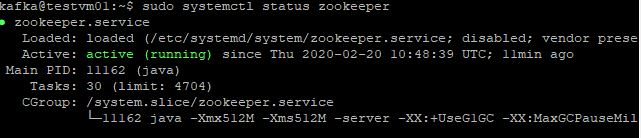
\includegraphics{images/StatusZookeeper}
	\caption{Status des Zookeeper-Dienstes nach dem Start}
	\label{img:StatusZookeeper}
\end{figure}

Für ein automatisches Starten des Dienstes nach einem Reboot führen Sie folgendes Kommando aus:

\smallskip

\begin{lstlisting}[language=Bash]
$ sudo systemctl enable zookeeper
\end{lstlisting}

Ab jetzt wird Zookeeper automatisch nach einem Neustart beim Hochfahren aller Systeme mit gestartet.

\textbf{Kafka-Dienst starten:}

\bigskip

Führen Sie die gleichen Befehle für den Start des Kafka-Dienstes durch. Achten Sie darauf, dass Sie in allen Befehlen \glqq zookeeper\grqq\ durch \glqq kafka\grqq\ als Dienstbezeichnung ersetzen.

\smallskip

Überprüfen Sie mit dem \glqq status\grqq\ -Befehl, ob der Dienst aktiv ist. Der Output sollte wie folgt aussehen:

\begin{figure}[h]
	\centering
	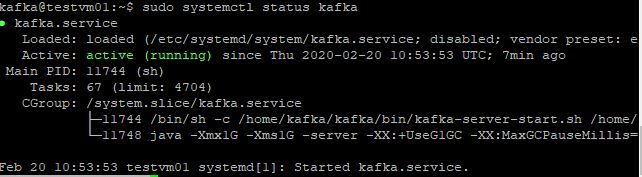
\includegraphics{images/StatusKafka}
	\caption{Status des Kafka-Dienstes nach dem Start}
	\label{img:StatusZookeeper}
\end{figure}

Nun sind Zookeeper und Kafka als Linux-Server-Dienst verfügbar ohne, dass ein Benutzer hierfür dauerhaft angemeldet sein muss.

\subsubsection*{Testen der Installation}

Um sicherzustellen, dass Kafka als Dienst korrekt läuft, wird eine \glqq HelloWorld\grqq\ -Nachricht produziert und konsumiert. Um eine Nachricht mittels Kafka zu versenden sind zwei Bestandteile nötig:

\begin{itemize}
\item Producer, welcher ein Topic registriert und Nachrichten produziert
\item Consumer, welcher Nachrichten aus dem Topic lesen kann
\end{itemize}

Hierfür werden die bei der Installation mitgelieferten Skripte im \glqq kafka\grqq\ -Verzeichnis benutzt.

Zuerst muss ein Topic erstellt werden. Das Topic heißt für Testzwecke \glqq Test\grqq.  Führen Sie folgenden Befehl aus:

\smallskip

\begin{lstlisting}[language=Bash]
$ ~/kafka/bin/kafka-topics.sh --create --zookeeper localhost:2181 --replication-factor 1 --partitions 1 --topic Test
\end{lstlisting}

Der Befehl benötigt den Zookeeper-Dienst mit dessen Portnummer (Standard-Port: 2181) als Argument, weil Zookeeper für die Verwaltung der Kafka-Instanzen benötigt wird. Ist das Topic erfolgreich erstellt, erscheint folgender Output auf der Kommandozeile: \glqq Created topic Test\grqq.

Um einen Producer zu starten, der als Nachricht \glqq HelloWorld\grqq\ produziert und dem Kafka-Dienst übergibt, führen Sie folgenden Befehl aus:

\smallskip

\begin{lstlisting}[language=Bash]
$ echo "Hello, World" | ~/kafka/bin/kafka-console-producer.sh --broker-list localhost:9092 --topic Test > /dev/null
\end{lstlisting}

Der Befehl produziert eine Nachricht für das Topic \glqq Test\grqq\ und übergibt die Nachricht an Kafka.

Der Consumer benötigt als Argument den Zookeeper Hostname und den Port (Standardport: 2181) und das Topic aus dem Nachrichten konsumiert werden sollen.

\smallskip

\begin{lstlisting}[language=Bash]
$ ~/kafka/bin/kafka-console-consumer.sh --bootstrap-server localhost:9092 --topic Test --from-beginning
\end{lstlisting}

Nach der Ausführung des Consumer-Skripts, sollte die Nachricht \glqq HelloWorld\grqq\ auf dem Bildschirm erscheinen. Ist das nicht der Fall, überprüfen Sie Ihre durchgeführten Schritte. Das Skript blockiert den Benutzerprozess, weil der Consumer weiterhin auf eintreffende Nachrichten wartet. Um das Skript abzubrechen verwenden Sie STR+C als Shortcut auf der Tastatur.

Kafka steht nun als Server-Dienst zur Verfügung. Kafka kann für seine Einsatzbereiche ab jetzt vollständig verwendet werden.

\pagebreak

\chapter{Einführung in Python Module für ejabberd und Apache Kafka}
\label{chap:pythonModule}

Dieses Kapitel gibt eine Einführung in die Python Module sleekxmpp, pykafka und kafka-python. Für die Umsetzung ist es wichtig, die Funktionsweise und die Möglichkeiten der Module zu kennen. Diese Module werden von der \acs{REST} \acs{API} benötigt, um Nachrichten zu versenden oder zu empfangen.


\section{Python Modul sleekxmpp als \acs{XMPP}-Client}
\label{sec:SleekxmppModul}

Damit die Flask Applikation mit ejabberd kommunizieren kann, wird ein Python Modul benötigt, dass als \acs{XMPP}-Client mit ejabberd interagieren kann. Eine Anforderung ist, dass das Modul leicht zu verwenden ist und möglichst viele auf \acs{XMPP}-basierenden Chatfunktionalitäten enthält. Die Programmiersprache Python bietet viele \acs{XMPP}-Clients von denen einige im Folgenden aufgelistet sind:

\begin{itemize}
\item aioxmpp
\item xmpppy
\item pyxmpp
\item jabberpy
\item sleekxmpp
\end{itemize}

Sie unterscheiden sich alle in der Ausführlichkeit der Dokumentation, im Funktionsumfang und in der Handhabbarkeit für Entwickler. Auch werden einige Module, wie zum Beispiel jabberpy, nicht mehr weiterentwickelt und gewartet. Sleekxmpp \cite{pythonSleekxmpp} verspricht im Gegensatz zu anderen \acs{XMPP}-Clients in Python einen großen Funktionsumfang, eine ausführliche Dokumentation und Flexibilität. Außerdem wird es häufig von Communities, wie \texttt{stackoverflow.com}, und in der Literatur \cite{definiteGuideXMPP} empfohlen. Aus diesen Gründen wird \texttt{sleekxmpp} für Entwicklung des eigenen \acs{IMS} verwendet. Die \acs{REST} \acs{API} soll \texttt{sleekxmpp} benutzen, mit der ejabberd-Plattform interagieren und kommunizieren zu können.

Das Modul \texttt{sleekxmpp} kann über den Python Paketmanager pip wie folgt installiert werden:

\texttt{pip install sleekxmpp}

\autoref{lst:sleekxmppClassExample} zeigt eine Klasse \texttt{EchoBot}, die das Modul sleekxmpp verwendet. Die Beispiele und Implementierungen halten sich an die Empfehlungen der Dokumentation von \texttt{sleekxmpp} \cite{pythonSleekxmpp}.

\begin{lstlisting}[language=python, caption={Vorbereitungen für die Verwendung des Moduls sleekxmpp}, label={lst:sleekxmppClassExample}]
from sleekxmpp import ClientXMPP
class EchoBot(ClientXMPP):

    def __init__(self, jid, passwd):
        super(EchoBot, self).__init__(jid, passwd)
        self.add_event_handler('session_start', self.start)
        self.add_event_handler('message', self.message)
\end{lstlisting}

Die Klasse \texttt{EchoBot} erbt von der Klasse \texttt{ClientXMPP} des \texttt{sleekxmpp} Moduls. Der Konstruktor erwartet als Argumente eine Jabber-ID und ein Passwort. Diese werden an den Konstruktor von \texttt{ClientXMPP} weitergereicht. Sie werden für den Verbindungsaufbau zum \acs{XMPP}-Server benötigt. Mit der Methode \texttt{add\_event\_handler} wird ein Event definiert und eine Referenz auf eine Methode angegeben. Die Methode wird ausgeführt, wenn das Event eintrifft. Empfängt der \acs{XMPP}-Client eine Nachricht über \acs{XMPP}, wird die Methode \texttt{self.message} aufgerufen. Innerhalb dieser sogenannten Callback Methoden, kann ein Entwickler benutzerdefinierte Abläufe im Code implementieren. Das bestätigt die Flexibilität von \texttt{sleekxmpp}.

Ein Beispiel für die Callback-Methode \texttt{start} zeigt \autoref{lst:sleekxmppCallbackStart}.

\begin{lstlisting}[language=python, caption={Beispiel: Callback-Methode des Moduls sleekxmpp}, label={lst:sleekxmppCallbackStart}]
def start(self, event):
    self.send_presence()
    self.get_roster()
\end{lstlisting}

Die Callback-Methode wird aufgerufen, nachdem eine Verbindung mit einem \acs{XMPP}-Server hergestellt ist. Sie benutzt vererbte Methoden von der Klasse \texttt{ClientXMPP}. Zuerst wird der Online-Status an den Server übermittelt und mit Hilfe der zweiten Methode die Kontaktliste des angemeldeten Benutzers vom Server heruntergeladen. Die gesammte Kommunikation zwischen \acs{XMPP}-Client und \acs{XMPP}-Server basiert auf den Richtlinien des \acs{XMPP}-Protokolls. Sleekxmpp abstrahiert aufwendige Formatkonvertierungen und die Umsetzung der Richtlinien. Es bietet dem Entwickler Schnittstellen und Methoden, um den \acs{XMPP}-Client einfach in Applikationen integrieren zu können.

Die benutzerdefinierte Klasse \texttt{EchoBot} kann wie folgt genutzt werden, siehe \autoref{lst:sleekxmppExampleUseEchoBot}.

\begin{lstlisting}[language=python, caption={Beispiel: Aufbau einer Verbindung zu einem \acs{XMPP}-Server mit sleekxmpp}, label={lst:sleekxmppExampleUseEchoBot}]
xmpp_client = EchoBot('testuser@ejabberd-server', 'passwort')
plugins = ['xep_0030', 'xep_0004', 'xep_0060', 'xep_0199']

for item in plugins:
    xmpp_client.register_plugin(item)

if xmpp_client.connect('10.10.8.10', 5222):
    t1 = threading.Thread(target=xmpp_client.process, kwargs={'block': True}, deamon=True)
    # send messages or do something else
    
    xmpp_client.disconnect(wait=True)
\end{lstlisting}

Zuerst wird eine Instanz der Klasse \texttt{EchoBot} erzeugt. Anschließend wird eine Liste mit benötigten \acs{XMPP}-Stanzas initialisiert. Zum Beispiel ermöglicht die \acs{XMPP}-Stanza XEP-0030 eine Service Discovery. Ein Client kann also verfügbare Dienste auf dem \acs{XMPP}-Server abfragen. XEP-0004 ruft Informationen über Datenformate und Datenaustausch vom Server ab. Genaue Details über XEP-Stanzas finden sich im offiziellen \acs{XMPP}-Definite Guide \cite{definiteGuideXMPP}. Die Stanzas werden anschließend in einer Schleife am \acs{XMPP}-Client registriert. Mit der Methode \texttt{connect} verbindet sich sleekxmpp unter Angabe von IP-Adresse und Port mit dem Server.  In der Dokumentation finden sich ausschließlich Beispiele, in denen die Methode \texttt{xmpp\_client.process(block=True)} aufgerufen wird. Das sleekxmpp-Objekt wartet dadurch auf eingehende Nachrichten. Die Konsequenz daraus ist, dass der sequentielle Programmablauf unterbrochen ist, weil der Haupt-Thread blockiert. Mit dem  Code-Konstrukt aus der Dokumentation ist es nicht möglich in einem Programm auf eingehende Nachrichten zu warten und nebenbei eine Nachricht zu versenden. Ein Problem, das später fatal wäre, für die Umsetzung des \acs{IMS}. Die Lösung ist, wie in \autoref{lst:sleekxmppExampleUseEchoBot} dargestellt, die Methode \texttt{process(block=True)} in einem eigenen Thread ausführen zu lassen. Dadurch kann eine Nachricht versendet werden, während auf eintreffende Nachrichten gewartet werden kann. Trifft eine Nachricht ein, wird kurz zur Callback-Methode gesprungen und diese ausgeführt.\cite{pythonSleekxmpp}

\pagebreak

\section{Python Module für Apache Kafka Client}
\label{sec:KafkaModul}

Wie die \acs{REST} \acs{API} mit ejabberd kommunizieren kann, ist bereits erläutert. Es stellt sich allerdings die Frage, wie die \acs{REST} \acs{API} mit der Apache Kafka-Instanz kommunizieren kann. Für Python sind Module verfügbar, die direkt mit Apache Kafka kommunizieren können.

\subsubsection*{Typische Module:}

\begin{itemize}
\item kafka-python
\item pykafka
\end{itemize}

In der Community von github wird pykafka für seine bessere Performanz gegenüber kafka-python gelobt. Auch ist es mehr mit für Python typische Implementierungsstrukturen entworfen, zum Beispiel asynchrones Fehlerhandling oder Benutzung von Kontext-Managern.\cite{pykafkaGithubMeaning}

\autoref{lst:pykafkaProducerExample} zeigt, wie der Producer des Moduls pykafka verwendet werden kann. Der Beispielcode schreibt die Nachricht \glqq hello world\grqq\ in das Kafka Topic \glqq test\grqq.

\begin{lstlisting}[language=python, caption={Beispiel: Verwendung des Producers des Moduls pykafka}, label={lst:pykafkaProducerExample}]
from pykafka import KafkaClient

kafka_client = KafkaClient(hosts='10.10.8.4:9092')
topic = kafka_client.topics['test']

with topic.get_producer() as kafka_producer:
    kafka_producer.produce(b'hello world')
\end{lstlisting}

Zuerst wird die Klasse \texttt{KafkaClient} importiert. Anschließend wird durch Aufruf des Konstruktors die Verbindung zur Kafka-Instanz hergestellt. Dem Konstruktor bekommt als Übergabeargument die IP-Adresse mit Port unter welcher die Apache Kafka-Instanz über das Netzwerk erreichbar ist. Danach wird das Topic definiert in das Nachrichten produziert werden sollen. Über das Topic und einem Kontext-Manager wird die Methode \texttt{produce} aufgerufen, die die Nachricht versendet. Sie erwartet ein Byte-Objekt. Ein e Nachricht vom Typ String in Python darf nicht übergeben werden.  Der Kontext-Manager sorgt für den automatischen Verbindungsauf- und abbau. Die Methode \texttt{get\_producer} sorgt, dafür, dass der Producer asynchron arbeitet. Die Methode \texttt{produce} wird sofort nach dem Versand der Nachricht verlassen, unabhängig davon, ob diese von der Kafka Instanz in das Topic geschrieben wird oder nicht. Diese Art von Producer eignet sich für das Versenden von großen Nachrichten. Das Modul kann allerdings auch über die Methode \texttt{get\_sync\_producer} einen Producer initialisieren, der solange blockiert, bis die Kafka-Instanz den Empfang der Nachricht quittiert hat.

Aus Gründen der Performanz wird \texttt{get\_producer} in der Studienarbeit genutzt.

Ein Consumer kann mit pykafka wie folgt implementiert werden (siehe \autoref{lst:pykafkaConsumerExample}).

\begin{lstlisting}[language=python, caption={Beispiel: Verwendung des Consumers des Moduls pykafka}, label={lst:pykafkaConsumerExample}]
from pykafka import KafkaClient

kafka_client = KafkaClient(hosts='10.10.8.4:9092')
topic = kafka_client.topics['test']
for i in topic.get_simple_consumer():
    print(i.value.decode())
\end{lstlisting}

Genau wie in \autoref{lst:pykafkaProducerExample}, wird zuerst eine Verbindung zur Kafka-Instanz hergestellt. Anschließend wird das Topic definiert, von dem der Consumer Nachrichten konsumieren soll. Über die Methode \texttt{get\_simple\_consumer} wird eine Consumer-Instanz erzeugt, über das mit einer Schleife iteriert werden kann. Der Consumer gibt alle Nachrichten auf der Konsole auf, die im Topic enthalten sind. Sind alle Nachrichten ausgegeben oder keine Nachrichten im Topic vorhanden, blockiert er sofort. Er wartet dann auf eintreffende Nachrichten und gibt die neu eingetroffenen Nachrichten aus. Dieser einfache Consumer hat folgenden Nachteil: Konsumieren mehrere Consumer aus dem gleichen Topic, konsumieren alle Consumer die gleichen Nachrichten. Mehrere Consumer können nicht dazu benutzt werden, die Geschwindigkeit der Verarbeitung von Nachrichten zu steigern. Ist das Anwendungsszenario aber nötig, empfiehlt die Dokumentation den Consumer, den die Methode \texttt{get\_balanced\_consumer} erzeugt.

Das Modul pykafka hat für die Implementierung des \acs{IMS} den Nachteil, dass es keine Topics auf Kafka-Instanzen angelegen kann. Jeder Benutzer des \acs{IMS} muss bei der Registrierung ein eigenes Topic erhalten. Würde alle Benutzer sich ein gemeinsames Topic teilen, würden alle Benutzer alle Nachrichten erhalten. Das sollte vermieden werden. Ein Producer eines konkreten Benutzers darf nur in ein bestimmtes Topic schreiben, wenn der Empfänger der Nachricht in seiner Kontaktliste enthalten ist. So können Nachrichten Punkt-zu-Punkt übertragen werden.

Aus diesem Grund ist die alleinige Benutzung von pykafka nicht möglich. Das Modul kafka-python enthält jedoch eine Klasse \texttt{KafkaAdminClient} über die sich Topics auf Kafka-Servern anlegen lassen. 

\pagebreak

\autoref{lst:kafkapythonAdmin} zeigt, wie ein Topic mit dem \texttt{KafkaAdminClient} angelegt werden kann.

\begin{lstlisting}[language=python, caption={Beispiel: Anlegen eines Topics mit dem KafkaAdminClient des Moduls kafka-python}, label={lst:kafkapythonAdmin}]
from kafka.admin import KafkaAdminClient, NewTopic

admin_client = KafkaAdminClient(bootstrap_servers='10.10.8.4:9092')
topics = [ NewTopic(name="example_topic", num_partitions=1, replication_factor=1) ]
try:
    admin_client.create_topics(new_topics=topics,validate_only=False)
except errors.TopicAlreadyExistsError as e:
    # handle error

\end{lstlisting}

Nachdem sich durch Aufruf des Konstruktors der Kafka Admin-Client mit dem Kafka-Server verbunden hat, wird mit Hilfe der Klasse \texttt{NewTopic} ein neues Topic erstellt. Das Topic erhält einen Namen, und die Anzahl an Partitionen die für das Topic reserviert werden sollen. Zusätzlich kann über den Replication Factor die Replizierung des Topics auf anderen Kafka-Brokern veranlasst werden. Eine \glqq 1\grqq\ bedeutet, dass das Topic nur auf einem Kafka-Broker angelegt wird. Das neue Topic wird in eine Liste eingefügt. Die Liste kann auch mehrere Topics enthalten. Über die Methode \texttt{create\_topic} werden die Topics aus der Liste angelegt. Existiert ein Topic auf dem Kafka-Broker bereits, wird eine Exception geworfen und der Vorgang abgebrochen.

Für die Studienarbeit werden beide Python Module eingesetzt und sich für die Implementierung an die Dokumentationen \cite{pykafkaDocumentation, pythonKafka} gehalten.

\pagebreak

\chapter{Umsetzung der Entwicklung einer \acs{REST} \acs{API}}
\label{chap:Backend}

Ausgangspunkt dieses Kapitels ist das Ergebnis der in \autoref{chap:Architektur} definierten Architektur. Dieses Kapitel befasst sich mit der Entwicklung der \acs{REST} \acs{API}. Es zeigt wichtige Aspekte und Ideen der Umsetzung mittels des Microframeworks Python Flask auf. Zu Beginn werden Anforderungen an die \acs{REST} \acs{API} und anschließend die genaue Umsetzung und der Programm-Code erläutert.

\subsubsection*{Anforderungen an die \acs{REST} \acs{API}:}

\begin{itemize}
\item Datenbankzugriffe
\item Authentifizierung der Benutzer
\item Schützen der Ressourcen vor nicht autorisiertem Zugriff
\item Bereitstellen von Chat-Funktionen über \ac{XMPP} und über Apache Kafka
\item Koordinierung des Nachrichtentransports von Clients zu benötigten Diensten des \ac{IMS}
\item Implementierung der Chat-Funktionen, die in der Weboberfläche vom Benutzer aufgerufen werden können.
\item Auslieferung von \ac{HTML}-, \ac{CSS}- und JavaScript-Dokumenten an den Browser des Clients
\item Fehlerbehandlung zum Beispiel bei invaliden Übergabeparametern
\end{itemize}

\section{Verbergen von Konfigurationsparametern der Flask Applikation}

Laut einer Statistik der Universität Maryland \cite{securityStatisticWebSites} werden Computer mit Internetzugriff alle 39 Sekunden von Hackern angegriffen. Die Statistik bestätigt, dass aufgrund dem hohen Risiko eines Angriffs, keine Leichtsinnigkeit bei der Implementierung vorhanden sein darf. Schon durch kleine Schwachstellen ist es Angreifern möglich, sensible Zugangsdaten abzugreifen und die Kontrolle über Systeme zu übernehmen. Aus diesem Grund sollten Zugangsdaten nicht direkt in Klartext im Programm-Code stehen. Die benötigten Zugangsdaten für ejabberd, Apache Kafka und den beiden MySQL-Datenbanken werden deshalb in einer separaten Datei im Datenaustauschformat \acs{JSON} abgespeichert. Die Flask Applikation soll beim Start alle Parameter auslesen und dynamisch verwenden. Auf diese Weise bleiben sensible Zugangsdaten geschützt, weil der Zugriff auf die separate Datei über das Betriebssystem auf wenige Benutzer beschränkt wird.

\autoref{img:configJSON-Datei} zeigt die Datei mit beispielhaften Zugangsdaten. Die Datei enthält alle wichtigen Informationen, wie IP-Adressen, Portnummern und alle Zugangsdaten für Apache Kafka, ejabberd und den beiden Datenbanken. Die Zugangsdaten für die Datenbank sind bereits im \acs{URI}-Format von SQLAlchemy eingetragen, sodass diese nicht erst durch zusätzlichen Programm-Code in das richtige Format gebracht werden müssen.

\begin{figure}[h]
	\centering
	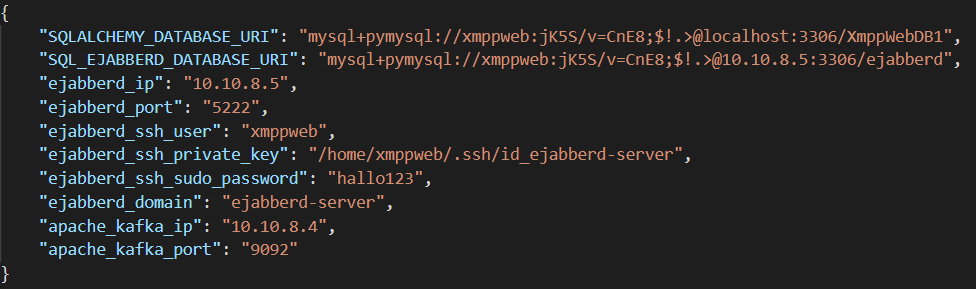
\includegraphics[width=\linewidth]{images/configJSON-Datei}
	\caption{Auszug aus der Konfigurationsdatei mit beispielhaften Zugangsdaten}
	\label{img:configJSON-Datei}
\end{figure}

Die Zugangsdaten sind in der Datei im Datenformat \ac{JSON} gespeichert, welches auf dem Name-Value-Prinzip basiert. Ein name (deutsch Name) bildet eindeutig auf einen value (deutsch Wert) ab. Maschinen verarbeiten das Datenformat schnell und einfach und für den Menschen ist es einfach lesbar. \ac{JSON} ist unabhängig von einer Programmiersprache.\cite{jsonIntroduction}

\autoref{lst:readConfigFile} zeigt einen Ausschnitt aus dem Code der Flask Applikation und wie die Konfigurationsparameter eingelesen werden können.

\begin{lstlisting}[language=python, caption={Auslesen der Konfigurationsparameter aus einer Datei}, label={lst:readConfigFile}]
with open("/home/xmppweb/config.json") as config_file:
    config = json.load(config_file)

app = Flask(__name__)
app.config['SQLALCHEMY_DATABASE_URI'] = config.get('SQLALCHEMY_DATABASE_URI')
app.config['SQLALCHEMY_BINDS'] = {
    "ejabberd_database": config.get('SQL_EJABBERD_DATABASE_URI') }
\end{lstlisting}

Mit dem Python Modul \texttt{json} und dessen Methode \texttt{load} können die Daten aus der Datei \texttt{config.json} importiert werden \cite{pythonJSONapi}. Die \texttt{load} Methode akzeptiert ein File-Objekt (hier \texttt{config\_file} genannt), der für das Einlesen einer Datei benötigt wird. Detaillierte Informationen über File-Objekte in Python 3 finden sich in der Dokumentation \cite{usageFileDeskr}. Gemäß der Konvertierungstabelle aus der Dokumentation \cite{pythonJSONapi} wird der Inhalt der Textdatei in das Datenformat Dictionary deserialisiert. Ein Dictionary in Python ist ein assoziatives Datenfeld und basiert ähnlich zu \ac{JSON} auf ein Key-Value-Prinzip. Über einen eindeutigen Key (deutsch Schlüssel) kann auf einem Value (deutsch Wert) zugegriffen werden. Das Dictionary aus \autoref{lst:readConfigFile} enthält die Konfigurationsparameter. Über die \texttt{get} Methode kann durch Angabe des Keys auf den Value zugegriffen werden. Für mehr Informationen über die Datenstruktur Dictionary, siehe \cite{pythonDictionaries}. So können die \acs{URI}s der beiden Datenbanken in die Konfiguration der Flask Applikation eingetragen werden.  Die Verwendung und der Zugriff auf die Konfigurationsparameter des Dictionaries wird in weiteren Listings benötigt. So kann zum Beispiel die IP-Adresse von Apache Kafka oder der ejabberd-Instanz dynamisch während der Laufzeit eingebunden werden, ohne dass diese direkt im Programm-Code sichtbar ist.

\section{SQLAlchemy Schema für die Benutzerauthentifizierung}

Für die Benutzerauthentifizierung und Registrierung von Benutzern am \acs{IMS} wird nach \autoref{img:logischeTopologieIMS} eine MySQL-Datenbank verwendet. Die MySQL-Datenbank läuft direkt als Dienst auf dem Server der Flask Applikation, um die Netzwerklatenz für Datenbankzugriffe möglichst gering zu halten. In der Tabelle \texttt{user\_auth} der Datenbank befinden sich alle Daten über die Benutzer. Weil alle Funktionalitäten des \acs{IMS} über die \acs{REST} \acs{API} koordiniert werden, muss ein SQLAlchemy Schema für den Zugriff auf die Tabelle erstellt werden. \autoref{lst:classUser} im Anhang definiert ein SQLAlchemy Schema für die Tabelle \texttt{user\_auth} und in \autoref{tab:descriptionUserClass} sind alle Spalten der Tabelle beschrieben. SQLAlchemy sorgt dafür, dass ein Entwickler im Programm-Code mit einem Objekt interagieren kann anstatt Tabellen mit SQL-Statements zu verändern. Die Attribute des SQLAlchemy Schemas entsprechen dabei den Spalten einer Tabelle. Durch das Schema ist SQLAlchemy die Struktur und die Daten, die in der Tabelle gesammelt werden sollen, bekannt. Alle Datenbankzugriffe und Netzwerkzugriffe abstrahiert SQLAlchmey für den Entwickler. Die Interaktion mit der Datenbank wird einfacher und die Flexibilität erhöht.

Die Klasse wird durch weitere Methoden erweitert, die in der Flask Appliaktion häufig verwendete Operationen implementieren. Das verhindert, das mehrfach der gleiche Code geschrieben und gewartet werden muss. Die Methoden werden im Folgenden kurz vorgestellt, weil sie in den \acs{API}-Routen der Flask Applikation häufig verwendet werden. Die Klasse erbt von der Klasse UserMixin des \texttt{flask\_login} Moduls, welches ein Python Modul darstellt, dass Login und Session Management vereinfacht. Die Methoden von \texttt{flask\_login} kann ein Entwickler in den Methoden der \acs{API}-Routen verwenden, um Benutzer ein- oder auszuloggen. Dieses Zusatzpaket vereinfacht die Entwicklung. Ein Entwickler muss keine Logik für den Login und dem Session-Management selbst entwickeln. Das Modul abstrahiert diese Art von Operationen und verbirgt diese hinter einfach zu benutzenden Schnittstellen. Genaue Informationen über die Verwendung findet sich in der offiziellen Dokumentation \cite{flaskLogin} des Moduls. Damit das Modul einen Benutzer eindeutig identifizieren kann und ihn korrekt ein- und ausloggen kann, muss nach \cite{flaskLogin} eine Methode \texttt{get\_id} innerhalb des Schemas definiert werden.

\autoref{lst:UserMethodFlaskLogin} zeigt die Implementierung.

\bigskip

\begin{lstlisting}[language=python, caption={Methode zur Identifizerung des Benutzers für das flask\_login Modul}, label={lst:UserMethodFlaskLogin}]
def get_id(self):
    return (self.user_id)
\end{lstlisting}

Das Attribut \texttt{user\_id} des User-Objekts entspricht der Spalte \texttt{user\_id} der Tabelle \texttt{user\_auth}. \texttt{user\_id} ist der Primärschlüssel der Datenbank und identifiziert eine Benutzer Entität eindeutig.

Damit ein Objekt der Klasse erzeugt werden kann, welches eine Identität der Tabelle \texttt{user\_auth} darstellt, muss ein Konstruktor definiert werden (siehe \autoref{lst:UserMethodConstructor}).

\bigskip

\begin{lstlisting}[language=python, caption={Konstruktor der Klasse User}, label={lst:UserMethodConstructor}]
    def __init__(self, user, email, passwd, topic_id, jabber_domain="@ejabberd-server"):
        self.username = user
        self.email = email
        self.passwd = self.__set_password(passwd)
        self.jabber_id = "{0}{1}".format(user, jabber_domain)
        self.kafka_topic_id = topic_id
\end{lstlisting}

Dem Konstruktor müssen alle Informationen über einen Benutzer übergeben werden. Die Beschreibung der einzelnen Daten einer Benutzer Entität befindet sich im Anhang in \autoref{tab:descriptionUserClass}. Der Konstruktor weißt beim Aufruf alle übergebenen Parameter den Attributen zu und erstellt das Objekt. Um zu verhindern, dass ein Passwort in Klartext oder eine falsche \texttt{jabber\_id} im User-Objekt gespeichert sein kann, formatiert der Konstruktor während der Initialisierung die Werte selbst. Mit Hilfe der \texttt{format}-Funktion kann ein Zeichensatz in eine benutzerdefinierte Form gebracht werden. Anwendungsbeispiele und Details befinden sich in \cite{pythonFormat}. Auf diese Weise wird die Jabber ID automatisch erzeugt. Sie ergibt sich durch Konkatenation aus Benutzername und der Jabber Domain. Die Konkatenation ergibt sich durch Anwenden der \texttt{format}-Funktion. Der formatierte Zeichensatz wird dann dem Attribut \texttt{jabber\_id} zugewiesen. Zum Beispiel ergibt sich aus dem Benutzernamen \texttt{testuser} und der Jabber ID \texttt{@ejabberd-server} die Jabber ID \texttt{testuser@ejabberd-server}. Das Passwort wird durch Aufruf der privaten Methode \texttt{set\_password} über eine Hashfunktion \footnote{Eine Hashfunktion H, enthält eine Eingabe des Alphabets beliebiger Länge (etwa ein Password) und erzeugt daraus einen Hashwert h fester Länge n = |h|, etwa ‘24988892bfc53b18b6d0fcc6ccbb9b59’.\cite{wendzel2018}} in einen Hashwert umgewandelt. \autoref{lst:UserMethodPasswordHash} zeigt die Implementierung dieser Methode.

\begin{lstlisting}[language=python, caption={Methode zur Berechnung des Password Hashes}, label={lst:UserMethodPasswordHash}]
def set_password(self, password, method="sha384"):
    if not type(password) == str:
        raise TypeError("expected a string as argument in set_password function.")
    return generate_password_hash(password, method=method)
\end{lstlisting}

\texttt{set\_password} verwendet die Methode \texttt{generate\_password\_hash} aus dem Python Modul werkzeug \cite{werkzeugDoc}. Das Modul erleichtert, die Erstellung eines Hashwerts, sodass der Entwickler selbst keine Hashfunktionen implementieren muss. Die Methode wirft eine Exception, falls das übergebene Password nicht vom Typ String (str) ist. Ansonsten wird das Passwort zusammen mit dem übergebenen Typ der Hashfunktion an \texttt{generate\_password\_hash} übergeben, die den Hashwert berechnet.

Das Python Modul werkzeug enthält zusätzlich eine Methode \texttt{check\_password\_hash}, die überprüft, ob ein in Klartext übergebener Zeichensatz mit einem gegebenen Hashwert übereinstimmt \cite{werkzeugDoc}. Die Klasse \texttt{User} verwendet diese Funktion gemäß \autoref{lst:UserClassVerifyMethod}.

\bigskip

\begin{lstlisting}[language=python, caption={Methode zur Überprüfung auf Übereinstimmung eines Zeichensatzes mit einem übergebenen Hashwert}, label={lst:UserClassVerifyMethod}]
def verify_password(self, password):
    return check_password_hash(self.passwd, password)
\end{lstlisting}

Die Methode \texttt{check\_password\_hash} berechnet dabei zuerst den Hashwert des in Klartext übergebenen Passworts. Anschließend überprüft es, ob der berechnete Hashwert mit dem übergebenen Hashwert übereinstimmt. Auf diese Weise kann ein User-Objekt, dass von der Datenbank über SQLAlchemy zurückgegeben wird, eine Methode anbieten, die sofort überprüfen kann, ob ein Passwort mit dem Passwort des Benutzers aus der Datenbank übereinstimmt. Der Rückgabeparameter ist vom Typ Boolean und ist True, falls die Hashwerte und damit die Passwörter übereinstimmen, ansonsten False.

\section{Umsetzung der Logins eines Benutzers}

Die Klasse \texttt{User} ist so modifiziert, dass sie Login Funktionalitäten unterstützt. Bevor die Methoden des \texttt{flask\_login} Moduls verwendet werden können, muss ein Flask-, SQLAlchemy- und Login-Manager-Objekt in der Flask Applikation instanziiert werden. (siehe \autoref{lst:flaskPrepareLogin}).

\begin{lstlisting}[language=python, caption={Vorbereitungen der Login Funktionalität in der Flask Applikation}, label={lst:flaskPrepareLogin}]
app = Flask(__name__)
db = SQLAlchemy(app)
login_mgmt = LoginManager(app)
login_mgmt.login_view = 'login'
\end{lstlisting}

Über das LoginManager-Objekt \texttt{login\_mgmt} können in der Flask Applikation Benutzer ein- und ausgeloggt werden. Das Objekt abstrahiert alle dafür benötigten Operationen und verwaltet die Sessions der Benutzer selbstständig. Das Modul vereinfacht die Implementierung eines Logins. Damit nicht angemeldete Benutzer, beim Zugriff auf eine geschützte Ressource zurück zur Login-Seite geleitet werden, wird \texttt{login\_view} entsprechend gesetzt. Zeile 4 in \autoref{lst:flaskPrepareLogin} definiert, dass die Methode \texttt{login} der Flask Applikation aufgerufen wird, wenn ein Benutzer, der nicht eingeloggt ist, auf eine geschützte Seite zugreift. Wie diese Methode funktioniert und implementiert ist, wird im weiteren Verlauf noch beschrieben.\cite{flaskLogin}

Der Login-Manager bietet die folgenden beiden Methoden für das Ein- und Ausloggen von Benutzen:

\begin{description}
\item[login\_user:] Loggt einen Benutzer ein. Benötigt als Übergabeargument ein User-Objekt.
\item[logout\_user:] Loggt einen Benutzer aus.
\end{description}

Bevor diese beiden Methoden im Code der Flask Applikation benutzt werden können, muss eine Callback Methode implementiert werden, die beim Ein- und Ausloggen von Benutzern aufgerufen wird. In \autoref{lst:UserClassCallback} ist die Implementierung der Callback Methode dargestellt.

\begin{lstlisting}[language=python, caption={Callback Methode für das Modul flask\_login}, label={lst:UserClassCallback}]
@login_mgmt.user_loader
def load_user(user_id):
    return User.query.get(int(user_id))
\end{lstlisting}

Die Methode lädt ein User-Objekt über die SQLALchemy Operation \texttt{query.get} aus der Datenbank und gibt es zurück. Die Wichtigkeit von Methode \texttt{get\_id} aus \autoref{lst:UserMethodFlaskLogin} zeigt sich in diesem Listing. Ohne diese Funktion, die die ID des User-Objekts zurückgibt, fehlt der Callback Methode der Parameter, der einen Benutzer eindeutig in der Datenbank identifiziert.\cite{flaskLogin}

Die vorgestellten Methoden des Login-Managers und der Klasse \texttt{User} können in der Flask Applikation genutzt werden, um Benutzer zu registrieren oder ein- und auszuloggen. So wird vermieden, dass an verschiedenen Stellen im Code mehrfach der gleiche Code programmiert wird.

Zusätzlich muss verhindert werden, dass bestimmte \acs{API}-Route von einem unangemeldeten Benutzer aufgerufen werden kann.

In \autoref{lst:flaskLoginProtectedDecorator} ist dargestellt, wie mit dem Login-Manager eine \acs{API}-Route vor unangemeldeten Benutzern geschützt werden kann.

\begin{lstlisting}[language=python, caption={Code für den Schutz der \acs{API}-Route vor unangemeldeten Benutzern}, label={lst:flaskLoginProtectedDecorator}]
@app.route("/gochat")
@login_required
def gochat():
    # code of the method gochat
\end{lstlisting}

Der Decorator \texttt{@login\_required} verhindert, dass ein Client die \acs{API}-Route aufruft, wenn er nicht über den Login-Manager bereits angemeldet ist. Der Mehrwert ist, dass ohne zusätzlichem Programmieraufwand, dafür gesorgt werden kann, dass nur angemeldete Benutzer die Chatfunktionalitäten des \acs{IMS} benutzen dürfen. Der Decorator muss nur über die Definition der \acs{API}-Routen eingefügt werden, welche nur von angemeldeten Benutzern aufgerufen werden dürfen.\cite{flaskLogin}

\pagebreak

\section{Umsetzung der Registrierung von Benutzern}

Für die Umsetzung wird folgende \acs{API}-Route definiert, unter der die Benutzerregistrierung möglich ist:

\texttt{http://193.196.53.24/register}

\autoref{img:umlActivityRegistration} im Anhang zeigt die Anwendungslogik für die Benutzerregistrierung, welche in einem \acs{UML} Aktivitätsdiagramm dargestellt ist. Ruft ein Client die oben definierte \acs{URI} auf, so wird eine Methode \texttt{register} in der Flask Applikation aufgerufen, in der diese Abläufe implementiert sind. Zuerst überprüft die Methode, ob der Benutzer bereits authentifiziert ist. Falls das der Fall ist, leitet die \acs{REST} \acs{API} den Client auf eine der Chatseiten um, für die sich der Benutzer des Clients bereits angemeldet hat. Die Chatseite kann entweder die der Kafka Plattform oder die der ejabberd Plattform sein. Greift der Client auf die \acs{URI} mit der \acs{HTTP} Basisoperation GET zu, findet keine Registrierung statt. Dem Client wird die \acs{HTML}-Seite ausgeliefert über die der Benutzer sich registrieren kann. Greift der Client mit einer \acs{HTTP} POST Anfrage auf die \acs{URI} zu, startet der Registrierungsprozess. Im ersten Schritt überprüft die Anwendungslogik, ob die vom Client gesendeten Daten, wie Benutzername, Passwort und weitere, im Datenaustauschformat \acs{JSON} vorliegen. Ferner wird überprüft, ob der Benutzer schon vorhanden ist. Falls nein, wird der Benutzer auf den beiden Chatplattformen ejabberd und Apache Kafka, sowie in der Tabelle \texttt{user\_auth} angelegt. Schlägt einer der drei Registrierungsprozesse fehl, werden nachfolgende Registrierungsschritte nicht ausgeführt. Außerdem hält die Anwendung bei einem Fehler die Datenbanken durch entsprechende Rollbacks und Fehlerbehandlung konsistent. Die Anwendungslogik verhält sich nicht korrekt, wenn der Server der Flask-Applikation während einem Registrierungsschritt aufgrund höherer Gewalt ausfällt. Eine Fehlerbehandlung in diesem Fall ist jedoch nicht Ziel dieser Studienarbeit. Ist der Benutzer auf beiden Plattformen und in der Tabelle der Benutzerdatenbank angelegt, ist der Registrierungsprozess erfolgreich.

Der Code für die Fehlerbehandlungen ist durch Conditional Code oder Exception Handling realisiert und eine Beschreibung des Codes bringt wenig Mehrwert. Es stellt sich aber die Frage, wie die drei Registrierungsschritte implementiert werden können.

Um einen Benutzer auf der \acs{XMPP}-basierten Plattform ejabberd anzulegen, könnte die \acs{REST} \acs{API} direkt in die MySQL-Datenbank der ejabberd-Instanz hineinschreiben. SQLAlchemy ist nach \autoref{lst:readConfigFile} bereits für den Zugriff auf die MySQL-Datenbank konfiguriert. Dagegen ist kritisch einzuwenden, dass in der offiziellen Dokumentation \cite{ejabberdDoc} keinerlei Informationen über den Aufbau des MySQL-Datenbankschemas vorhanden sind und Informationen über verwendete Hashfunktionen von Passwörtern unbekannt sind. Auch ist der Algorithmus für die Erzeugung der Salt\footnote{Salt: zufällig gewählte Zeichenfolge, die an einen gegebenen Klartext vor dessen weiterer Verarbeitung in einer Hashfunktion angehängt wird, um die Entropie der Eingabe zu erhöhen.\cite{wendzel2018}} Zeichenfolge unbekannt und nicht beschrieben. Die Flask Applikation kann aus diesen Gründen nicht direkt einen neuen Benutzer in die Datenbank von ejabberd anlegen. Nach dem Netzplan in \autoref{img:ArchitekturIMS} ist der Server der Flask Applikation direkt über das private Netzwerk \texttt{internalDMZ} mit der ejabberd-Instanz verbunden. Zudem lässt sich auf der ejabberd-Instanz nach \autoref{lst:AddAdminUserEjabberd} ein neuer Benutzer über das Kommandozeilenprogramm \texttt{ejabberdctl} in der Datenbank anlegen. Die Flask Applikation könnte sich über \ac{SSH} auf die ejabberd-Instanz verbinden und \texttt{ejabberdctl} direkt benutzen. Hierzu wird ein Benutzer auf dem Linux-System der ejabberd-Instanz angelegt, der die benötigten Rechte besitzt, um das Kommandozeilenprogramm \texttt{ejabberdctl} zu benutzen. Auf dem Linux-Server der Flask Applikation wird der gleiche Benutzer angelegt und zwischen dem ejabberd-Server und dem Server der Flask Applikation eine Public-Key-Authentifizierung über \ac{SSH} konfiguriert. So kann sich die Flask Applikation beim Aufbau der \ac{SSH}-Verbindung sicher authentifizieren, ohne ein Passwort eingeben zu müssen.

Dieser Ansatz lässt sich leicht mit dem Python Modul \texttt{subprocess} umsetzen \cite{pythonSubprocess}. Mit \texttt{subprocess} lassen sich Prozesse auf dem Betriebssystem starten und nach deren Ausführung die Return-Codes des Prozesses abfragen. Zusätzlich lassen sich Eingabe-, Ausgabe- und Fehlernachrichtenströme des Prozesses auslesen. Die Grundidee ist, eine Klasse \texttt{UserManagement} zu programmieren, die das Modul \texttt{subprocess} verwendet, um einen Benutzer in der Datenbank von ejabberd anlegen oder löschen zu können. Mit \texttt{subprocess} lässt sich der \ac{SSH}-Befehl von Linux in einem eigenen Prozess starten und das Unterprogramm \texttt{ejabberdctl} über \ac{SSH} ausführen, siehe \autoref{img:subprocesSSH}.

\begin{figure}[h]
	\centering
	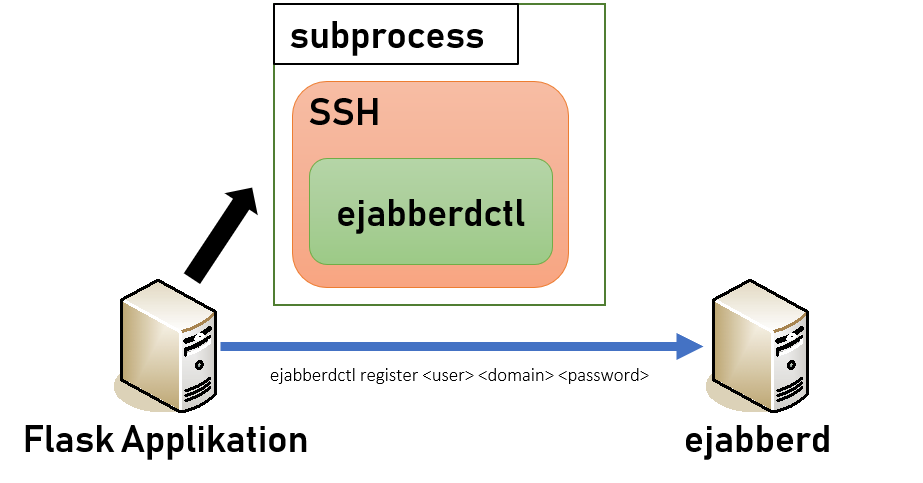
\includegraphics[width=.8\linewidth]{images/subprocessSSH}
	\caption{Grundidee der Benutzerregistrierung auf ejabberd mittels subprocess, eigene Darstellung}
	\label{img:subprocesSSH}
\end{figure}

\pagebreak

Um einen Benutzer \texttt{testuser} mit dem Passwort \texttt{hallo123} anzulegen, muss \texttt{subprocess} folgenden Befehl ausführen:

\texttt{echo “sudo\_password“ | ssh –tt –i $~$/.ssh/private\_key 10.10.8.10 “sudo ejabberdctl register testuser ejabberd-server hallo123“
}

\textbf{Bemerkung:} \texttt{ejabberdctl} kann nur mit erweiterten Rechten auf dem Linux-System ausgeführt werden, weshalb das sudo-Passwort mit angegeben werden muss.

\autoref{lst:UserManagementSubprocess} zeigt, wie dieser Befehl in der Methode \texttt{create\_user\_remotely} der Klasse \texttt{UserManagement} mit \texttt{subprocess} implementiert werden kann.

\begin{lstlisting}[language=python, caption={Methode create\_user\_remotely der Klasse UserManagement}, label={lst:UserManagementSubprocess}]
def create_user_remotely(self, username, passwd, server_domain):
    COMMAND = f"echo \"{self.sudo_passwd}\" | ssh -tt -i {self.private_key} {self.host} \"sudo ejabberdctl register {username} {server_domain} {passwd}\""

    result = subprocess.Popen(COMMAND, shell=True, stdout=subprocess.PIPE, stderr=subprocess.PIPE)

    stdout, stderr = result.communicate()
    return result.returncode
\end{lstlisting}

Die Variablen \texttt{sudo\_passwd}, \texttt{private\_key} und \texttt{host} sind Attribute der Klasse, welche dem Konstruktor mit übergeben werden müssen. Das Kommando (COMMAND) mit seinen variablen Parametern wird mit einem Python f-String formatiert und dynamisch generiert. Anschließend öffnet die Methode \texttt{Popen} von \texttt{subprocess} einen neuen Prozess und führt den Befehl aus. Mittels \texttt{communicate} interagiert \texttt{subprocess} mit dem erzeugten Prozess und extrahiert Informationen und Return Code aus den Nachrichtenströmen des Prozesses. Die Methode gibt dem Aufrufer den Return Code des Prozesses zurück. Falls der \texttt{ejabberdctl}-Befehl auf dem Remote-Server oder der Prozess selbst nicht erfolgreich ausgeführt werden konnte, ist der Return Code ungleich null. Der Aufrufer bekommt über den Return Code also Feedback über die Registrierung des Benutzers.

In der Klasse \texttt{UserManagement} ist ebenfalls eine Methode implementiert, die der Aufrufer benutzen kann, um einen Benutzer auf der ejabberd-Plattform zu löschen. Die Methode hilft Inkonsistenzen zu vermeiden. Der Aufbau ist sehr ähnlich zu der Methode in \autoref{lst:UserManagementSubprocess}, nur, dass das Kommando ein \texttt{unregister} anstatt \texttt{register} und auf die Angabe des Passworts verzichtet werden muss.

Ein Objekt der Klasse \texttt{UserManagaement} kann in der Methode \texttt{register} der \ac{API}-Route benutzt werden, um in der Datenbank von ejabberd einen neuen Benutzer zu registrieren.

\pagebreak

Den Code für die Methode \texttt{register} der Flask Applikation zeigt \autoref{lst:flaskRegisterCode}.

\begin{lstlisting}[language=python, caption={Code der \acs{API}-Route für die Benutzerregistrierung}, label={lst:flaskRegisterCode}]
@app.route("/register", methods=["GET", "POST"])
def register():
    ### error handling, consistency checks ###

    user_reg_obj = UserManagement(config['ejabberd_ip'], config['ejabberd_ssh_user'],priv_key=config['ejabberd_ssh_private_key'], sudo_passwd=config['ejabberd_ssh_sudo_password'])
    return_code=user_reg_obj.create_user_remotely(req_content["username"], req_content["password"], config["ejabberd_domain"])
    if return_code != 0:
        # error handling

    topic_id = str(uuid.uuid4())
    kafka_admin_client = KafkaAdminClient(bootstrap_servers=f'{config["apache_kafka_ip"]}:{config["apache_kafka_port"]}')
    topic_list = [NewTopic(name=topic_id, num_partitions=1, replication_factor=1)]
    kafka_admin_client.create_topics(new_topics=topic_list,validate_only=False)
    user = User(req_content["username"], req_content["eMail"], req_content["password"], topic_id)
    db.session.add(user)
    db.session.commit()
    
    ### error handling ###
\end{lstlisting}

Der \acs{JSON}-Payload ist bereits deserialisiert und befindet sich im Dictionary \texttt{req\_content}. In diesem Dictionary sind Informationen wie Benutzername, Passwort, E-Mail-Adresse und weitere enthalten, die zum Anlegen des Benutzers benötigt werden. Im Dictionary \texttt{config} sind alle Zugangsdaten der Konfigurationsdatei. Der Code beinhaltet alle drei notwendigen Registrierungsschritte. Zuerst wird ein Objekt der Klasse \texttt{UserManagement} erzeugt und mit Hilfe dieser Klasse der Benutzer auf der ejabberd-Plattform angelegt. Mit Hilfe des Return Codes dieser Operation, kann im Falle eines Fehlers weitere Registrierungsschritte verhindert werden. Die Methode dann wird vorzeitig verlassen und eine Antwort an den Client gesendet. Anschließend wird eine 36-stellige Topic ID mit dem Python Modul \texttt{uuid} zufällig erzeugt. Die Topic ID wird für das Anlegen eines Benutzers auf der Kafka-Plattform benötigt. Kafka kann keine Benutzer verwalten, jedoch Topics, welche Nachrichten speichern. Ein Topic wird einem Benutzer zugeordnet. So besitzt jeder Benutzer seinen eigenen Chatkanal und andere Benutzer empfangen keine Nachrichten von diesem Benutzer. Das Python Modul \texttt{kafka-python} \cite{pythonKafka} beinhaltet eine Klasse \texttt{KafkaAdminClient} mit dem ein neues Topic auf einer Kafka-Instanz angelegt werden kann. Nach \autoref{img:ArchitekturIMS} kann die Flask Applikation eine Verbindung über das Netzwerk zur Kafka Plattform herstellen. Als Server erwartet der Konstruktor des \texttt{KafkaAdminClient} die IP-Adresse der Kafka-Instanz. Anschließend kann über die Methode \texttt{create\_topics} ein neues Topic angelegt werden. Sie erwartet eine Liste mit \texttt{NewTopic}-Objekte als Argument, welche ebenfalls das Python Modul \texttt{kafka-python} bereitstellt. Das Modul wirft eine Exception, falls ein Topic bereits vorhanden ist oder eine Verbindung nicht möglich ist (Fehlerbehandlung nicht dargestellt). Als letzten Registrierungsschritt muss der Benutzer zur Datenbank auf der Flask-Instanz hinzugefügt werden, denn diese vermeidet die Benutzer-Accounts des \ac{IMS} für die Webapplikation. Dazu wird ein Objekt des SQLAlchemy-Schemas \texttt{User} angelegt und über SQLALchemy Operationen in die Datenbank eingefügt. Treten Fehler bei Registrierungsschritten auf, sorgt die Fehlerbehandlung dafür, dass Schritte rückgängig gemacht werden oder nachfolgende Registrierungsschritte nicht mehr ausgeführt werden. Der Datenbestand bleibt konsistent.

\section{Globales Dictionary für die Umsetzung von Chatfunktionalitäten}

Für das Senden und Empfangen von Nachrichten werden die in \autoref{sec:SleekxmppModul} und \autoref{sec:KafkaModul} vorgestellten Python Module verwendet. Es stellt sich jedoch die Frage, wie die Objekte der Module für jeden Benutzer isoliert verwendet werden können. Die Methode, die aufgerufen wird, wenn ein Client auf eine bestimmte \acs{API}-Route zugreift, hat einen lokalen Namensraum. Alle Objekte und Variablen werden nach verlassen der Methode gelöscht. Die Probleme, bereits beim Login von Benutzern entstehen, zeigt \autoref{lst:flaskProblemLocalNamespace}. Der Codeumfang des \autoref{lst:flaskProblemLocalNamespace} ist auf die Darstellung der resultierende Probleme reduziert. Die sich daraus ergebenen Probleme können analog auf die Verwendung des Moduls für die Apache Kafka Plattform übertragen werden.

\begin{lstlisting}[language=python, caption={Problem für Chatfunktionalitäten aufgrund des lokalen Namensraums von Methoden}, label={lst:flaskProblemLocalNamespace}]
@app.route("/login", methods=["GET", "POST"])
def login():
	# code to login user into session management...
	sleekxmpp_object = EchoBot("user1@ejabberd-server", "hallo123")
	# code to prepare connection
	if sleekxmpp_object.connect("10.10.8.10", 5222):
		# code to listen for new messages
\end{lstlisting}

Nachdem der Erstellung des \texttt{sleekxmpp}-Objekts, wird eine Verbindung mit dem \acs{XMPP}-Server hergestellt werden. Anschließend folgt der Code aus \autoref{lst:sleekxmppExampleUseEchoBot}, indem mittels eines Thread-Objekts auf eintreffende Nachrichten gewartet wird. Das kann aber nur solange geschehen, bis das \texttt{sleekxmpp}-Objekt beim Verlassen der Methode wieder zerstört wird. Damit erreicht der Thread sein natürliches Ende. Nachdem müssen aber solange Empfangen werden können, bis sich ein Benutzer ausloggt. Versendet ein Client durch Aufruf einer anderen \acs{API}-Route eine Nachricht, muss diese wieder ein \texttt{sleekxmpp}-Objekt erzeugen und die Nachricht versenden. Nach Verlassen des lokalen Namensraums der Methode ist das Objekt wieder zerstört. Es ist ineffizient ein Objekt ständig neu zu erzeugen, das nur eine sehr kurze Zeit, nämlich dem Versenden der Nachricht, benötigt wird.

Das Objekt für kurze Operationen nicht dauernd erzeugen zu müssen, verbessert diese Situation. Eine Möglichkeit ist, das Objekt beim Login als globale Variable zu initialisieren. Auf diese Weise kann das Objekt von anderen Methoden wiederverwendet und auf eingehende Nachrichten bis zum Logout des Benutzers gewartet werden. Dagegen ist kritisch anzumerken, dass ein anderer Benutzer, der sich ebenfalls am \acs{IMS} anmeldet, das Objekt mit seinem erzeugten Objekt überschreibt. Denn einem Benutzer gehört eine Jabber-ID und das \texttt{sleekxmpp}-Objekt meldet sich über das Netzwerk mit Jabber-ID und Passwort am \acs{XMPP}-Server an. Ein Objekt kann nicht mehrere Verbindungen über mehrere Jabber-IDs verwalten \cite{pythonSleekxmpp}.

Es ist also nach einer Möglichkeit gesucht, mit der Objekte wiederverwendet werden können und jeder Benutzer seine eigenen Objekte benutzt. Zusätzlich dürfen die Aktionen eines angemeldeten Benutzers die Aktionen eines anderen Benutzers nicht beeinflussen.

Ein globales Dictionary das in der Datei der Flask Applikation angelegt wird, kann für jeden Benutzer ein eigenes Objekt speichern.

Dieser Code initalisiert ein leeres Dictionary:

\texttt{session\_dict = \{\}}

Im Datentyp Dictionary bildet ein Schlüssel eindeutig auf einen Wert ab. Dieser Wert kann wieder ein Dictionary sein. Es ist eine Verschachtelung zulässig.\cite{pythonDictionaries}

Das Dictionary enthält Informationen über den aktuell angemeldeten Benutzer und wird deshalb in dieser Studienarbeit auch häufig als Session-Dictionary bezeichnet. Der Begriff in dieser Arbeit bezeichnet dieses Dictionary.

Ein Benutzer wird eindeutig über den Primärschlüssel in der Datenbank identifiziert. Der Primärschlüssel ist eine Ganzzahl. Diese Ganzzahl, welche auch als ID bezeichnet werden kann, kann als Schlüssel im Dictionary verwendet werden. Die ID als Schlüssel ist eindeutig und verweist dann auf ein weiteres Dictionary, dass alle für den angemeldeten Benutzer relevanten Daten speichert.

\pagebreak

\autoref{img:sessionDict} zeigt das Dictionary mit Beispieleinträgen.

\begin{figure}[h]
	\centering
	
\includegraphics[width=.6\textwidth]{images/sessionDict}
	\caption{Beispiel: Einträge in das globale Dictionary für Chatfunktionalitäten, eigene Darstellung}
	\label{img:sessionDict}
\end{figure}

Das Session-Dictionary zeigt einen Zustand, in dem zwei Benutzer am \acs{IMS} angemeldet sind. Die ID der beiden Benutzer aus der Datenbank wird als Schlüssel verwendet. Die beiden Benutzer sind für unterschiedliche Plattformen angemeldet. Der Benutzer testuser1 benutzt das Apache Kafka System für den Nachrichtentransport und der Benutzer testuser2 die \acs{XMPP}-basierte Plattform über ejabberd. Wichtig ist, dass für jeden Benutzer ein eigenes Objekt gespeichert wird, sodass kein Objekt überschrieben werden kann. Je nachdem, für welche Plattform sich ein Benutzer angemeldet hat, wird ein Objekt des entsprechenden Python-Clients unabhängig von anderen Benutzern unabhängig gespeichert. Zusätzlich können in diesem Dictionary auch noch weitere Informationen, wie zum Beispiel für welche Plattform ein Benutzer angemeldet ist.

Der Vorteil ist folgender:

Im Code von Methoden der \acs{API}-Routen kann durch Conditional Code unterschieden, welche Plattform der Benutzer benutzt. Dadurch kann eine \acs{API}-Route für beide Plattformen verwendet werden. Es muss nicht für jede Plattform eine extra \acs{API}-Route definiert werden. Die Fehlerbehandlung und die Überprüfungen sind zum Beispiel für den Versand von Nachrichten für beide Plattformen gleich. Das Frontend muss für beide Plattformen dieselbe Anfrage und denselben Payload versenden. Auf diese Weise kann Code gespart werden. Das vereinfacht die Wartung der Software. Code muss im Falle von Änderungen nur an einer Stelle geändert werden. Das reduziert die Fehleranfälligkeit.

Ein weiterer Vorteil ist, dass auf die Daten in dem verschachtelten Dictionary schnell zugegriffen werden kann. Ein Dictionary bietet einen Zugriff auf einen Wert in der Geschwindigkeitsklasse O(1) \cite{pythonSpeed}. Bekommt die \acs{API} von einem Client den Auftrag, für einen Benutzer eine Nachricht zu versenden, kann sie gezielt auf das Objekt des Benutzers zugreifen und die Nachricht an die jeweilige Plattform senden.

\textbf{Beispiel:} \texttt{session\_dict[32]['xmpp\_object'].send\_message(...)}

Das Session-Dictionary ist in \autoref{img:sessionDict} nicht vollständig abgebildet. In dieser Arbeit wird das Dictionary um weitere Daten erweitert, wenn das für die Funktionen des \acs{IMS} notwendig ist.

\section{Beschreibung der \acs{API}-Route des Logins}

Für einen Login am \ac{IMS} wird folgende \acs{API}-Route definiert:

\texttt{http://193.196.53.24/login}

\autoref{img:umlActivityLogin} im Anhang zeigt die Anwendungslogik der Flask Applikation vom Login eines Benutzers. Verbindet sich ein Benutzer mit seinem Client auf die oben genannte \acs{URI} wird eine Methode \texttt{login} der Flask Applikation aufgerufen, in der diese Abläufe implementiert sind. Ist ein Benutzer bereits eingeloggt und in der \acs{REST} \acs{API} authentifiziert, leitet die \acs{API} den Benutzer auf die Chatseite um, für die der Benutzer bereits authentifiziert ist. Greift der Client auf die \acs{URI} mit der Basisoperation \acs{HTTP} GET zu, findet keine Anmeldung am System statt. Dem Client wird die \acs{HTML}-Seite durch die \acs{API} ausgeliefert, über die der Benutzer sich anmelden kann. Greift der Client mit der Basisoperation \acs{HTTP} POST auf die \acs{URI} zu, startet der Anmeldevorgang. Zuerst wird überprüft, ob der Benutzername in der Datenbank vorhanden ist und das vom Client gesendete Passwort mit dem Passwort-Hash aus der Datenbank übereinstimmt. Falls nein, sind die Daten im \acs{JSON}-Payload invalide und der Benutzer wird über eine Fehlermeldung informiert. Anhand des Werts, auf den der Name \texttt{requested\_platform} im \acs{JSON}-Payload verweist, wird unterschieden, ob ein Benutzer über die \acs{XMPP}-basierte Plattform oder über die Apache Kafka Plattform kommunizieren möchte. Je nach gesetztem Eintrag, benutzt die \acs{API} entweder einen \acs{XMPP}-Client oder einen Apache Kafka Client als Python Modul, um Nachrichten empfangen und versenden zu können. Hat sich die Flask Applikation mit dem korrekten Python Client an einen der beiden Plattformen erfolgreich eingeloggt, muss die \ac{API} den Benutzer noch im Session-Management des Login-Managers einloggen. So weiß die \acs{API}, welcher Benutzer gerade am \acs{IMS} angemeldet ist und welche Plattform dieser benutzt.

\pagebreak

Den Code für den Loginvorgang zeigt \autoref{lst:flaskLoginCode}.

\begin{lstlisting}[language=python, caption={Code der \acs{API}-Route für den Benutzerlogin}, label={lst:flaskLoginCode}]
@app.route("/login", methods=['GET', 'POST'])
def login():
    # error handling code
    user = User.query.filter_by(username=req_content["username"]).first()
    if not user or not user.verify_password(req_content["password"]):
        # send errors and exit
    if req_content.get('requested_platform') == 'xmpp':
        xmpp_client = create_sleekxmpp_client(user, req_content)

        if xmpp_client.connect((config.get("ejabberd_ip"), config.get("ejabberd_port"))):
            t1 = threading.Thread(target=xmpp_client.process, kwargs={'block': True}, daemon=True)
            t1.start()
            login_user(user, remember=req_content["remember"])
            # send successfull message and exit
        # if not taken -> send errors and exit
    elif req_content.get('requested_platform') == 'kafka':
        kafka_client = get_kafka_client()
        kafka_producer = kafka_client.topics[user.kafka_topic_id].get_producer()
        # error handling
        global session_dict
        session_dict[user.user_id] = {"kafka_producer_object": kafka_producer, "topic": user.kafka_topic_id, "requested_platform": "kafka"}
        login_user(user, remember=req_content["remember"])
        # send successfull message or handle errors and exit
    else:
        # send errors and exit
\end{lstlisting}

Im Dictionary \texttt{req\_content} befindet sich der vom Client an die \acs{API} übertragene Payload, der die Informationen für die Anmeldung enthält. Im Dictionary \texttt{config} sind Konfigurationsparameter und Zugangsdaten bereits eingelesen. Die \acs{REST} \acs{API} überprüft zuerst, ob der Benutzer in der Datenbank vorhanden ist. Hierzu verwendet sie die SQLAlchemy Operation \texttt{query.filter\_by}, mit der die Tabelle \texttt{user\_auth} durchsucht werden kann. Gesucht wird nach dem ersten auffindbaren Eintrag, der dem Benutzernamen entspricht. Anschließend wird überprüft, ob die SQLAlchemy Operation ein User-Objekt zurückgegeben hat und ob das übermittelte Passwort mit dem Passwort-Hash aus der Datenbank übereinstimmt. Falls das der Fall ist, wird anhand des Wertes, auf dem der Schlüssel \texttt{requested\_platform} aus dem Payload verweist, entschieden, für welche Plattform sich der Benutzer anmelden möchte. Fordert der Client die Plattform \texttt{xmpp} an, erzeugt die Methode \texttt{create\_sleekxmpp\_client} ein Objekt des Python \texttt{sleekxmpp}-Clients und gibt es an den Aufrufer zurück. Sie fügt es in das globale Session-Dictionary bereits ein. Außerdem erzeugt sie eine zufällige Zeichenfolge, welche zusätzlich in das Session-Dictionary eingefügt wird. Diese wird später für den Empfang von Nachrichten benötigt und im weiteren Verlauf der Arbeit erläutert. Im nächsten Schritt wird ein Verbindungsaufbau zur ejabberd-Instanz mit Hilfe des \acs{XMPP}-Clients gestartet. Falls dieser erfolgreich ist, wird mit Hilfe des Python Moduls \texttt{threading} \cite{pythonThreading} ein Thread gestartet, der dauerhaft auf den Empfang von Nachrichten wartet. Sofern keine Fehler aufgetreten sind, kann das \texttt{sleekxmpp}-Objekt aus dem globalen Session-Dictionary von anderen Methoden für den Nachrichtenversand verwendet werden. Der gestartete Thread wartet im Hintergrund auf eingehende Nachrichten. Über die Methode \texttt{login\_user} des Login-Managers wird der Benutzer an der \acs{REST} \acs{API} angemeldet und ins Session-Management des Login-Managers aufgenommen.
Meldet sich der Client für die Plattform Kafka an, wird mit Hilfe des Python Moduls \texttt{pykafka} ein Producer-Objekt erzeugt und in das globale Session-Dictionary eingefügt. Methoden, die Nachrichten versenden, können das Producer-Objekt direkt verwenden. Zusätzlich wird die Topic ID darin gespeichert, sodass ein Producer anhand des globalen Session-Dictionary weiß, wie die Topic ID des Benutzers lautet, an dem er die Nachricht senden möchte. Dieser Sachverhalt wird im Verlauf der Arbeit noch genauer erläutert. Genau wie beim Anmeldevorgang an die \acs{XMPP}-basierte Plattform wird am Ende des Codeabschnitts der Benutzer über \texttt{login\_user} an der \acs{REST} \acs{API} angemeldet.

\textbf{Bemerkungen:} Fehlerbehandlungen und Exception-Handling sind in \autoref{lst:flaskLoginCode} bewusst aufgrund von Unübersichtlichkeit nicht dargestellt. Die \acs{REST} \acs{API} informiert den Benutzer jedoch über Fehler.

\pagebreak

\section{Laden des Chatverlaufs bei Benutzung der \acs{XMPP}-basierten Plattform}

Die \acs{API} muss einem Client den Nachrichtenverlauf übermitteln können. Der Client kann den Nachrichtenverlauf über die \acs{URI} \texttt{193.196.53.24/get\_messages} erhalten.  Die Nachrichten werden bei der \acs{XMPP}-basierten Plattform von ejabberd direkt in seiner MySQL-Datenbank gespeichert.

\autoref{img:ejaberdChatHistory} zeigt einen Ausschnitt mit relevanten Spalten aus der Tabelle, in der die Chatverläufe von ejabberd gespeichert werden. Die Inhalte aus der Spalte xml sind auf die notwendigen Informationen begrenzt.

\begin{figure}[h]
	\centering
	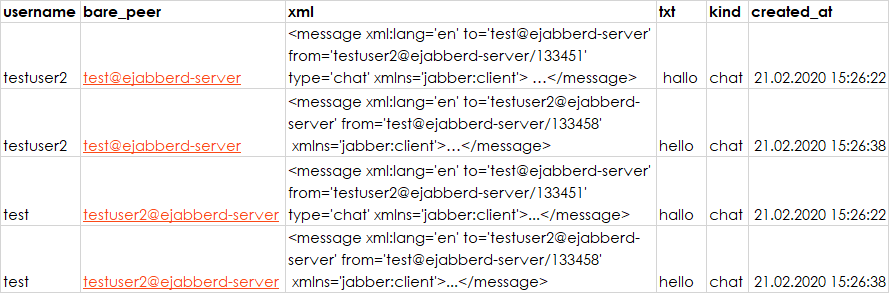
\includegraphics[width=\textwidth]{images/ejabberdChatHistory}
	\caption{Aufbau der Tabelle der Chatverläufe von ejabberd, eigene Darstellung}
	\label{img:ejaberdChatHistory}
\end{figure}

Die \acs{API} muss den Chatverlauf aus der Tabelle direkt exportieren und in das Datenformat \acs{JSON} konvertieren. Das \acs{JSON}-Objekt mit den Chatverläufen kann einem Client dann zurückgegeben werden. Die Struktur der Tabelle entspricht nicht den Design-Prinzipien von relationalen Datenbanken. Die Nachrichten in der Tabelle sind redundant gespeichert. Zum Beispiel wird die gleiche Nachricht, die testuser2 an test schickt, von den beiden Chatpartnern jeweils einmal gespeichert. Die Nachrichten in Zeile 1 und 3, sowie in Zeile 2 und 4 sind jeweils gleich. Hinzu kommt, dass die Tabelle keine optimale Struktur besitzt, um anhand der Informationen in einer Spalte zu entscheiden, wer welche Nachricht gesendet und empfangen hat und zu welchem Chatverlauf eine Nachricht gehört. Ein einfacher Export des Chatverlaufs zwischen zwei Benutzern ist nicht möglich. Mit einem typischen SELECT-Befehl der Sprache \acs{SQL} ist es nicht möglich alle Chatverläufe für jeden Benutzer zu extrahieren.

Eine mögliche Lösung ist, die Eindeutigkeit der Spalte xml zu verwenden. Die Spalte xml speichert die Nachricht im Datenformat \acs{XML}. In diesem Format überträgt das \acs{XMPP}-Protokoll die Nachricht zwischen Client und Server. Die Attribute from und to einer Nachricht verweisen eindeutig auf die Jabber-ID und damit auf den Benutzer, der die Nachricht versendet oder empfangen hat. Ein Chatverlauf ist zwischen zwei Kommunikationspartnern kann mit Hilfe der Spalten username, bare\_peer und und dem Attribut from aus dem \acs{XML} eindeutig aus der Tabelle extrahiert werden.

Einen Algorithmus der diesen Ansatz nutzt, zeigt \autoref{lst:flaskExtractXMPPChathistory}.

\begin{lstlisting}[language=python, caption={Code für die Generierung des Chatverlaufes von ejabberd}, label={lst:flaskExtractXMPPChathistory}]
def get_chat_history(username):
    POSITION_XML = 1
    chat_rosters_bare_peers = Archiv.query.with_entities(Archiv.bare_peer).filter_by(username=username).group_by("bare_peer").all()
    chat_msgs = {}
    for bare_peer in chat_rosters_bare_peers:
        list_peer_msgs = []
        results = Archiv.query.with_entities(Archiv.txt, Archiv.xml, Archiv.created_at, Archiv.kind).filter_by(username=username).filter_by(bare_peer=bare_peer[0]).all()
        for item in results:
            match = re.findall(regex, item[POSITION_XML])
            list_peer_msgs.append({"txt": item[0], "timestamp": item[2].strftime('%Y-%m-%d %H:%M:%S'), "type": item[3], "from": match[0]})
        list_peer_msgs_sorted = list(sorted(list_peer_msgs, key=lambda k: k["timestamp"]))
        chat_msgs[bare_peer[0].split('@')[0]] = list_peer_msgs_sorted
    return chat_msgs
\end{lstlisting}

Die Methode implementiert eine Klasse \texttt{Archiv}, die ein SQLAlchemy Schema darstellt und den Aufbau der Tabelle von ejabberd beschreibt, die die Chatverläufe speichert. So kann SQLAlchemy auf die Tabelle der Datenbank von ejabebrd zugreifen. Das Schema ist aus Gründen der Vollständigkeit im Anhang \autoref{lst:flaskClassArchiv} abgebildet, eine Beschreibung bietet jedoch wenig Mehrwert. Vielmehr wird im Folgenden der Algorithmus beschrieben, den diese Klasse implementiert.
Die Methode akzeptiert einen Benutzernamen und extrahiert den gesamten Chatverlauf des Benutzers mit seinen Kommunikationspartnern. Zu Beginn extrahiert eine SQLAlchemy Operation alle Chatpartner des Benutzers.
Ein mögliches Ergebnis des Benutzers testuser2 sieht wie folgt aus:

\texttt{[('test@ejabberd-server',),('testuser3@ejabberd-server',)]}

Die SQLAlchemy Operation gibt eine List mit Tupeln zurück, die alle Benutzer enthält, mit denen testuser2 kommuniziert. Die Anzahl der Elemente der Liste entspricht der Anzahl der Chatverläufe.

In den folgenden Erläuterung wird ausschließlich gezeigt, wie der Chatverlauf des Benutzers mit dem Kommunikationspartner \texttt{test@ejabberd-server} extrahiert wird. Die Methode muss die Vorgänge jedoch für jeden Chatpartner ausführen, sodass am Ende ein Chatverlauf von allen Kommunikationspartnern entsteht.

Im nächsten Schritt muss für jeden Chatpartner der Nachrichtenverlauf mit einer SQLALchemy Operation abgefragt werden. Der Chatverlauf zwischen dem Benutzer und dem Chatpartner aus der Liste wird in der Variablen \texttt{results} gespeichert. Die Methode \texttt{with\_entities} teilt SQLAlchemy mit, dass nur die Spalten, die als Argumente übergeben sind, abgefragt werden sollen. Die relevanten Spalten sind: txt, xml, created\_at, kind. Die Bedeutung der Spalten ergibt sich aus \autoref{img:ejaberdChatHistory}. Zurückgegeben wird eine Liste von Tupeln, die alle Nachrichten des Kommunikationsverlaufs enthält.

Stellt man die Ergebnisse in einer Tabelle dar, ergibt sich \autoref{img:ejabberdChatHistoryWithoutRedundancy}:

\begin{figure}[h]
	\centering
	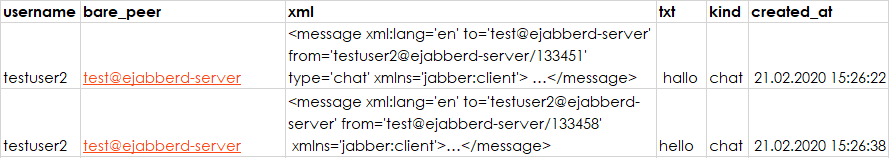
\includegraphics[width=\textwidth]{images/ejabberdChatHistoryWithoutRedundancy}
	\caption{Darstellung der Chatverläufe von ejabberd mit entfernten Redundanzen, eigene Darstellung}
	\label{img:ejabberdChatHistoryWithoutRedundancy}
\end{figure}

Im Vergleich zu \autoref{img:ejaberdChatHistory} sind alle redundanten Informationen entfernt. Das Ergebnis beinhaltet nicht mehr die redundant gespeicherten Nachrichten aus der Sicht von jedem Benutzer.

Über die Spalte xml lässt sich über eine Regex\footnote{Mittels einer Regex können Zeichenketten durch Angabe eines Patterns aus einer Zeichenkette extrahiert werden.\cite{pythonRegex}} in Python, die Jabber-ID des Attributs from extrahieren. Anhand des from Attributs kann der Absender der Nachricht genau zugeordnet werden. Zum Beispiel lässt sich anhand des Attributs from in Zeile von \autoref{img:ejabberdChatHistoryWithoutRedundancy} sagen, dass die Nachricht \glqq hallo\grqq, von testuser2 stammt und der Benutzer test der Empfänger dieser Nachricht ist.

Auf diese Weise baut der Algorithmus ein Dictionary für jede Nachricht, in der alle wichtige Informationen, wie Absender, Empfänger, Art der Nachricht (Einzel- oder Gruppenchat) und Zeitstempel der Nachricht enthalten sind.

Die einzelnen Dictionaries werden dann in eine Liste eingefügt. Die Liste entspricht dann dem Chatverlauf zwischen zwei Benutzern.

\pagebreak

Das Ergebnis des Chatverlaufs zwischen den Benutzern testuser2 und test aus \autoref{img:ejabberdChatHistoryWithoutRedundancy} sieht wie folgt aus:

\texttt{[\{'txt': 'hallo', 'timestamp': '2020-02-21 15:26:22', 'type': 'chat', 'from': 'testuser2'\},} \\ \texttt{\{'txt': 'hello', 'timestamp': '2020-02-21 15:26:38', 'type': 'chat', 'from': 'test'\}]}

Damit der Nachrichtenverlauf zeitlich in der richtigen Reihenfolge gespeichert ist, wird die Liste nach dem Zeitstempel sortiert, siehe Zeile 11 in \autoref{lst:flaskExtractXMPPChathistory}.

Diesen Ablauf muss die Methode für jeden Chatpartner durchlaufen. Die daraus erhaltenen Chatverläufe müssen noch in einem übergeordneten Dictionary \texttt{chat\_msgs} eingefügt werden. So enthält das Dictionary den Chatverlauf des Benutzers zu jedem Kommunikationspartner.

Ein Beispiel des gesamten Nachrichtenverlaufs von testuser2 sieht wie folgt aus (siehe \autoref{img:ejabberdExampleFullChathistory}):

\begin{figure}[h]
	\centering
	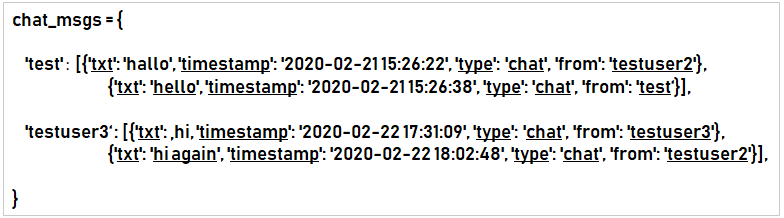
\includegraphics[width=\textwidth]{images/ejabberdExampleFullChathistory}
	\caption{Beispiel: Gesamter Chatverlauf eines Benutzers von ejabberd, eigene Darstellung}
	\label{img:ejabberdExampleFullChathistory}
\end{figure}

Die Namen der Chatpartner bilden als Schlüssel im Dictionary eindeutig auf den Chatverlauf ab. Das funktioniert, weil der Name des Chatpartners in der Flask Applikation gemäß \autoref{lst:classUser} eindeutig sein muss.

Ein Client oder die Webanwendung kann sich nun auf die \acs{URI} \texttt{193.196.53.24/get\_chathistory} verbinden, um den gesamten Nachrichtenverlauf im Datenaustauschformat \acs{JSON} abzufragen. Das Dictionary das den gesamten Chatverlauf enthält kann über die Methode \texttt{jsonify} des Flask Moduls in ein JSON-Objekt leicht umgewandelt werden:

\texttt{jsonify(chat\_msgs)}

\pagebreak

Der Mehrwert des vorgestellten Algorithmus ist, das ein Client den Chatverlauf in einer geordneten Struktur erhält und selbst entscheiden kann, in welcher Formatierung die Nachrichten dem Benutzer angezeigt werden. Außerdem ist über das Key-Value-Prinzip schnell auf den Chatverlauf des Benutzers mit einem bestimmten Kommunikationspartner zugreifbar:

\texttt{chat\_msgs['test']} oder \texttt{chat\_msgs['testuser3']}

\pagebreak

\section{Umsetzung des Senden von Nachrichten in der \acs{API}}

Die \acs{REST} \acs{API} versendet Nachrichten entweder an ejabberd oder Apache Kafka,je nachdem welche Plattform ein Benutzer verwendet. Der Client muss hierfür mit der Basisoperation \acs{HTTP} POST einen Auftrag an die \acs{URI} \texttt{http://193.196.53.24/send\_message} senden.

\autoref{img:requestExampleSendMessages} zeigt den Payload der Anfrage im \acs{JSON}-Format.

\begin{figure}[h]
	\centering
	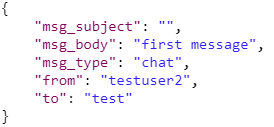
\includegraphics[width=.5\textwidth]{images/requestExampleSendMessages}
	\caption{Beispiel: \acs{JSON}-Payload für das Versenden Nachrichten, eigene Darstellung}
	\label{img:requestExampleSendMessages}
\end{figure}

Die \acs{API} benötigt alle Angaben, um eine Nachricht versenden zu können. Der Paremeter from verweist auf den Benutzer, welcher die Nachricht absendet, der Parameter to auf den Benutzer, an welchen die Nachricht versendet werden soll. In \texttt{msg\_body} steht die Nachricht und in \texttt{msg\_subject} der Betreff der Nachricht. Dieser kann, wie in \autoref{img:requestExampleSendMessages} dargestellt, auch leer sein. Er wird nur für den Versand einer Nachricht mit dem \acs{XMPP}-Client benötigt, aber nicht für die Kommunikation mit Apache Kafka. Falls in der Zukunft auch ein Gruppenchat realisiert wird, kann \texttt{msg\_type} dazu verwendet werden, den Typ der Nachricht zu einzuordnen.

Im Anhang in \autoref{img:umlActivitySendMessage} ist die Anwendungslogik in einem \acs{UML}-Aktivitätsdiagramm dargestellt. Sendet ein Client eine \acs{HTTP} POST Anfrage, wird zuerst überprüft, ob der Benutzer des Clients bereits im \acs{IMS} eingeloggt ist. Falls nein, sendet die \acs{API} dem Client eine Benachrichtigung im \acs{JSON}-Format. Falls Einträge im \acs{JSON}-Payload der POST Anfrage fehlen oder invalide sind, sendet die \acs{API} dem Client ebenfalls entsprechende Benachrichtigungen. Ein Nachrichtenversand ist nur möglich, wenn der Benutzers des Clients eingeloggt ist und die Parameter im Payload gültig sind. Danach unterscheidet die \acs{API} anhand des Parameters \texttt{requested\_platform} für welche Plattform der Benutzer angemeldet ist und sendet die Nachricht mit dem entsprechenden Python Client - entweder mit dem sleekxmpp-Client oder über den pykafka-Client. Treten Fehler auf, wenn eine Nachricht versendet wird, informiert die \acs{API} den Client über eine Nachricht im \acs{JSON}-Format.

Wie der Versand einer Nachricht im Code der \acs{API} umgesetzt ist, wird im Folgenden beschrieben:

Die \acs{API} muss unterscheiden, für welche Plattform ein Benutzer angemeldet ist. Das kann durch Conditional Code entschieden werden.

\autoref{lst:selectedPlatformCode} zeigt, wie die \acs{API} entscheidet, über welche Plattform die Nachricht versendet werden soll.

\begin{lstlisting}[language=python, caption={Code für den Versand einer Nachricht über die \acs{API} an ejabberd}, label={lst:selectedPlatformCode}]
if session_dict[current_user.user_id]['requested_platform']=='xmpp':
	# send message via sleekxmpp object
    # if no errors -> send successfull feedback to client
elif session_dict[current_user.user_id]['requested_platform']=='kafka':
    # send message with pykafka producer
    # if no errors -> send successfull feedback to client
else:
    # send error -> no valid plattform
\end{lstlisting}

Die \acs{API} nutzt die Einträge aus dem Session-Dictionary. Der Aufruf \texttt{current\_user.user\_id} ist eine Funktion des Login-Managers, der die ID des Benutzers zurückgibt, der diese Operation gerade aufruft. Zurückgegeben wird die ID des Benutzers aus der Tabelle user\_auth, welche die Benutzerinformationen speichert. Die ID ist, wie in vorherigen Abschnitten beschrieben, der Primärschlüssel der Tabelle und verweist eindeutig auf den Benutzer. Der Login-Manager benutzt diese ID, um die Sessions von Benutzern zu verwalten. Weil die ID eines Benutzers im Session-Dictionary als Schlüssel benutzt wird, kann die \acs{API} direkt auf die Einträge des Benutzers im Session-Dictionary zugreifen und verwenden. Durch diese Überprüfung versendet die \acs{API} die Nachricht an die richtige Plattform im Backend.

\autoref{lst:flaskSendMessage} zeigt, wie die Nachricht versendet wird, wenn der Benutzer für die Plattform ejabberd angemeldet ist.
%TODO gleiches caption wie vorheriges?
\begin{lstlisting}[language=python, caption={Code für den Versand einer Nachricht über die \acs{API} an ejabberd}, label={lst:flaskSendMessage}]
# if-part of Listing 5.44
if session_dict[current_user.user_id]['requested_platform']=='xmpp':
    session_dict[current_user.user_id]["xmpp_object"].push_message(JSON_Data["to"]+"@ejabberd-server", JSON_Data["msg_body"], JSON_Data["msg_subject"], JSON_Data["msg_type"])
    # if no errors -> send successfull feedback to client
\end{lstlisting}


In {JSON\_Data} sind die Parameter enthalten, die der Client an die \acs{API} über die POST Anfrage übermittelt hat.
Über das Session-Dictionary ruft die \acs{API} die Methode des sleekxmpp-Objekts auf, um die Nachricht zu versenden. Jeder Benutzer hat sein eigenes sleekxmpp-Objekt im Session-Dictionary. Das Versenden einer Nachricht beeinflusst keine anderen Objekte oder Einträge im Dictionary. Der Methode wird der Benutzername konkateniert mit der ejabberd-Domain, die Nachricht, der Betreff und der Typ der Nachricht übergeben. Diese Informationen benötigt das Modul sleekxmpp, um Nachrichten über \acs{XMPP} versenden zu können. Die Kontaktlisten der Benutzer pflegt und verwaltet ejabberd in seiner eigenen MySQL-Datenbank. Ejabberd prüft selbstständig, ob ein Benutzer mit einem anderen Benutzer kommunizieren darf. Es ist keine zusätzliche Verwaltung durch die \acs{API} nötig.

Anders ist die Situation, wenn die Nachricht über die Apache Kafka Plattform versendet werden soll:

Apache Kafka verwaltet die Topics von Benutzern, aber nicht die Kontaktliste eines Benutzers. Hierzu muss in der MySQL-Datenbank, die die Flask Applikation benutzt, eine Tabelle erstellt werden, die jedem Benutzer einen Chatpartner zuordnet. Die Beziehung zwischen den Benutzern im \acs{IMS} ist eine Many-To-Many-Relationship. In deutscher Literatur wird eine Many-To-Many-Relationship auch als m:m-Beziehung bezeichnet \cite{Schubert2007}. Nach Schubert \cite{Schubert2007} besteht zwischen zwei Entitätenklassen E1 und E2 genau dann eine m:m-Beziehung, wenn zu jedem Exemplar aus E1 mehrere Exemplare der Entitätenklasse E2 gehören können und umgekehrt. Im \acs{IMS} kann ein Benutzer von mehreren Benutzern als Kontakt hinzugefügt werden genauso, wie er selbst mehrere Benutzer als Kontakt hinzufügen kann. Die Besonderheit ist, dass in diesem Fall die Entitätenklassen E1 und E2 gleich sind und beide die Entitätenklasse Benutzer repräsentieren.

In \autoref{tab:tableContacts} ist die Tabelle contacts mit Einträgen dargestellt.

\begin{table}[h]
\centering
\caption{Übersicht über die Tabelle contacts für die Speicherung von Chatpartnern für die Plattform Apache Kafka}
\begin{tabular}{|l|l|}
\hline
\textbf{user\_id} &  \textbf{peer\_id} \\
\hline
41 & 32 \\
\hline
41 & 12 \\
\hline
32 & 41 \\
\hline
12 & 41 \\
\hline
... & ... \\
\hline
\end{tabular}
\label{tab:tableContacts}
\end{table}

Die Tabelle beinhaltet die IDs aus der Tabelle \texttt{user\_auth} der Datenbank (siehe Anhang \autoref{lst:classUser} und \autoref{tab:descriptionUserClass}) als Fremdschlüssel. Wie in vorherigen Kapiteln erwähnt, speichert die Tabelle \texttt{user\_auth} die Benutzer des \acs{IMS}. Sowohl die Spalte \texttt{user\_id} und \texttt{peer\_id} sind aufgrund der m:m-Beziehung zwischen den Benutzern Primärschlüssel in \autoref{tab:tableContacts}. Die ID eines Benutzers bildet eindeutig auf die ID eines anderen Benutzers ab, welcher sein Chatpartner ist. Die Zuordnung gilt auch umgekehrt. Weil die Kommunikation in einem \acs{IMS} bidirektional ist, muss ein Eintrag für beide Richtungen gesetzt werden, wenn ein Benutzer jemanden als Kontakt hinzufügt, siehe \autoref{tab:tableContacts}.

Die contacts hat den Mehrwert, dass die \acs{API} vor dem Versenden einer Nachricht über die Apache Kafka Plattform überprüfen kann, ob die Benutzer Chatpartner sind.

Der Code für den Versand einer Nachricht über die Apache Kafka Plattform ist in \autoref{lst:flaskSendMessageKafka} dargestellt.

\begin{lstlisting}[language=python, caption={Code für den Versand einer Nachricht über die \acs{API} an Apache Kafka}, label={lst:flaskSendMessageKafka}]
# elif-part of Listing 5.44
elif session_dict[current_user.user_id]['requested_platform']=='kafka':
# check in table contacts if chat partners exists
# return error as JSON if chat partners does not exist
# get kafka topic id of chat partner through a join with table user_auth
# peer_kafka_topic stores the kafka topic id of the chat partner
msg_timestamp = datetime.today().strftime('%Y-%m-%d %H:%M')
msg = {"msg": JSON_Data['msg_body'], "from": JSON_Data['from'], "to": JSON_Data['to'], "timestamp": msg_timestamp, "type": "chat"}
session_dict[current_user.user_id]['kafka_producer_object'].produce(json.dumps(msg).encode())

if peer_id in session_dict:
session_dict[peer_id]['kafka_producer_object'].produce(json.dumps(msg).encode())
else:
kafka_client = get_kafka_client()
topic = kafka_client.topics[peer_kafka_topic]
with topic.get_producer() as kafka_producer:
    kafka_producer.produce(json.dumps(msg).encode())
\end{lstlisting}

In \texttt{JSON\_Data} sind die Parameter des Payloads aus der \acs{HTTP} POST Anfrage.
Zuerst überprüft die \acs{API} mit Hilfe der in \autoref{tab:tableContacts} dargestellten Tabelle contacts, ob dem Sender der Empfänger als Chatpartner zugeordnet ist. Dafür muss ein Eintrag in der Tabelle contacts existieren. Weil in \texttt{JSON\_Data} nur der Benutzername des Absenders und des Empfängers vorhanden sind, muss über ein Join\footnote{Ein Join bildet aus den Datensätzen zweier Tabellen einer relationalen Datenbank eine Ergebnistabelle, deren Datensätze, je nach angegebener Bedingung, Attribute beider Tabellen enthält.\cite{Schubert2007}} mit der Tabelle user\_auth festgestellt werden, ob ein Eintrag in der Tabelle contacts existiert. Falls nein, darf die Nachricht nicht versendet werden und die \acs{API} antwortet dem Client mit einem Fehler im \acs{JSON}-Format. Sind die beiden Benutzer Chatpartner, wird über das Session-Dictionary der Producer des Empfängers aufgerufen und die Nachricht in sein spezielles Topic produziert. Zusätzlich wird der Producer des Senders aus dem Session-Dictionary aufgerufen und die Nachricht ebenfalls an den Sender verschickt. So haben Sender und Empfänger immer einen synchronisierten Chatverlauf.

Die Vorgehensweise funktioniert nur, wenn Sender und Empfänger gleichzeitig online sind. Ist der Empfänger offline, ist kein Eintrag im Session-Dictionary und damit kein Producer-Objekt vorhanden. Dann muss ein Producer-Objekt manuell erzeugt werden und die Nachricht in das Topic des Empfängers produziert werden. Die Topic ID des Empfängers wird in diesem Fall über den bereits beschriebenen Join aus der Datenbank abgefragt. Der Versand der Nachricht ist optimiert für den Fall, dass der Empfänger ebenfalls online ist. Es muss kein Producer-Objekt extra erzeugt werden. Producer-Objekt und Topic ID werden aus dem Session-Dictionary direkt verwendet (Zeile 12 in \autoref{lst:flaskSendMessageKafka}). Nur wenn der Empfänger der Nachricht offline ist, muss ein Producer-Objekt auf Kosten der Performanz erzeugt werden (Zeile 16 in \autoref{lst:flaskSendMessageKafka}).

\textbf{Bemerkung:} \texttt{json.dumps(msg).encode()} konvertiert das Dictionary \texttt{msg} in einen Byte-Code. So kann ein \acs{JSON}-Objekt in ein Topic produziert werden.

\section{Umsetzung der Zustellung von empfangenen Nachrichten an den Client}

Die \acs{REST} \acs{API} kommuniziert mit Apache Kafka oder mit ejabberd über bestimmte Python Module. Es stellt sich jedoch die Frage, wie die Nachricht dem Client des \acs{IMS} übermittelt wird. Empfängt die \acs{API} eine Nachricht, muss sie die Nachricht direkt dem Client oder zum Web-Frontend weiterleiten ohne, dass der Client ständig nach neuen Nachrichten am Flask-Server anfragen muss. Dieser Mechanismus wird als Server Push bezeichnet. Bei einem Server Push \cite{sseVSwebsockets} hält ein Client die Verbindung zum Server dauerhaft offen. Der Server schickt den Client über diese Verbindung automatisch Informationen ohne, dass der Client explizit beim Server anfragen muss. Dieser Mechanismus wird für die Umsetzung in der Studienarbeit benötigt, weil ansonsten der Informationsfluss unterbrochen ist und keine Echtzeitübertragung von Nachrichten möglich ist. Der Client müsste ohne diesen Mechanismus nach einer Zeitspanne t beim Server anfragen, ob neue Nachrichten vorhanden sind. Falls ja, überträgt der Server die neuen Nachrichten und der Client verarbeitet diese. Ein \acs{IMS} besitzt jedoch eine gewisse Echtzeitfähigkeit, weshalb dieser Ansatz zu verwerfen ist.

Zwei Webtechnologien, mit denen ein Server Push umgesetzt werden kann, sind \cite{sseVSwebsockets}:

\begin{itemize}
\item Web Sockets
\item \ac{SSE}
\end{itemize}

Über Web Sockets ist eine bidirektionale Kommunikation zwischen Client und Server möglich. Ein Server kann einem Client Nachrichten senden und umgekehrt auch Nachrichten vom Client über den Web Socket empfangen. Client und Server können ohne Unterbrechungen miteinander kommunizieren, solange die Verbindung bestehen bleibt.\cite{sseVSwebsockets}

Bei \ac{SSE}s kann nur der Server dem Client Informationen senden \cite{sseMorzilla, sseVSwebsockets}. Die Verbindung ist unidirektional. In \autoref{img:SSE-Architecture} ist ein Ablauf eines Server-Sent-Events zwischen Client und Server dargestellt.

\begin{figure}[h]
	\centering
	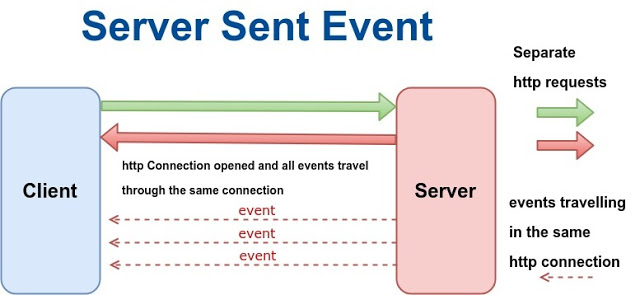
\includegraphics[width=.8\textwidth]{images/SSE-Architecture}
	\caption{Ablauf eines Server-Sent-Events \cite{sseFunctionGraphic}}
	\label{img:SSE-Architecture}
\end{figure}

Der Client erhält in Echtzeit automatisch Informationen vom Server. Die Informationen gehören zu einem Event. Der Client empfängt Informationen für ein oder mehrere Events.\cite{sseMorzilla, sseVSwebsockets}

Gemeinsamkeiten von beiden Technologien sind, dass beide über das \acs{HTTP}-Protokoll kommunizieren und sie lang andauernde Verbindungen zwischen Client und Server benutzen.

Ein Nachteil von \acs{SSE}s ist, dass eine geringere Anzahl an Browsern mit \acs{SSE}s als mit Web Sockets kompatibel sind. Ein Vorteil ist, dass \acs{SSE}s bei einer unterbrochenen Verbindung zwischen Server und Client automatisch erneut eine Verbindung herstellen.\cite{sseMorzilla}

Für die Studienarbeit wird ausschließlich eine unidirektionale Verbindung vom Server zum Client benötigt. Der Client versendet seine Nachrichten, wie im vorherigen Abschnitt erklärt mit einer \acs{HTTP} POST Anfrage. Eine Verbindung vom Client zum Server wird deshalb nicht gebraucht. Aus diesem Grund werden \acs{SSE}s verwendet, um die Nachrichten den Clients zuzustellen.

Daten, die der Server dem Client über ein \acs{SSE} sendet, müssen immer als Zeichensatz in UTF-8 kodiert sein und wie folgt formatiert sein \cite{sseMorzilla}:

\texttt{data: <Daten>\escape{n}\escape{n}}

Zusätzlich muss das serverseitige Skript, das Ereignisse sendet, mit dem \acs{MIME}-Typ\footnote{ Der MIME-Typ gibt an, um welche Art oder Klasse es sich bei den gesendeten Daten handelt.\cite{mimeTypDescription}} \glqq text/event-stream\grqq\ dem Client antworten \cite{sseMorzilla}.

In Python Flask lassen sich Server-Sent-Events mit Generatoren realisieren. Generatoren in Python sind Funktionen, die Werte generieren und an den Aufrufer zurückgeben. Sie enthalten anstatt einer \texttt{return}-Anweisung ein \texttt{yield}. Ein Generator ist ein Objekt über das iteriert werden muss, um einen Wert zu erhalten. Die \texttt{yield}-Instruktion gibt den momentanen Wert zurück.

\autoref{lst:pythonGeneratorExample} zeigt ein Beispiel eines Generators. Der Code gibt zeilenweise die Zahlen 1 bis 10 auf der Konsole aus.

\begin{lstlisting}[language=python, caption={Beispiel: Code für ein Generator Objekt in Python}, label={lst:pythonGeneratorExample}]
def myfunction(x):
    for i in range(10):
        yield x
        x += 1
for i in myfunction(1):
    print(i)
\end{lstlisting}

Der Generator erzeugt zehn Werte und inkrementiert den übergebenen Wert x bis die Abbruchbedingung zutrifft. Im Unterschied zu einer Funktion mit \texttt{return}-Anweisung kann sich ein Generator den Zustand von Variablen nach jeder Iteration merken. Der Generator in \autoref{lst:pythonGeneratorExample} gibt nach jeder Iteration einen Wert zurück ohne, dass der aktuelle x-Wert wie bei einer \texttt{return}-Anweisung verloren geht.

Eine \acs{API}-Route in Flask kann einen Generator benutzen, um ein Server-Sent-Event zu implementieren. Ein Beispiel zeigt \autoref{lst:pythonGeneratorFlaskExample}.

\begin{lstlisting}[language=python, caption={Beispiel: Code für ein Server-Sent-Event in Python Flask}, label={lst:pythonGeneratorFlaskExample}]
from flask import Flask, Response
app = Flask(__name__)
def myfunction(x):
    for i in range(10):
        yield "data: %s\n\n" % x
        x += 1

@app.route('/')
def print_x():
    return Response(myfunction(1), mimetype="text/event-stream")
\end{lstlisting}

Die \texttt{Response}-Funktion von Flask aus \autoref{lst:pythonGeneratorFlaskExample} akzeptiert ein Generator-Objekt. Ruft ein Client die  \acs{URI} / auf, so startet das Server-Sent-Event und sendet dem Client die Zahlen 1 bis 10.

Diese Funktionalität von Flask kann genutzt werden, um einem Client Nachrichten auszuliefern.

Die Architektur dieser Lösung verdeutlicht \autoref{img:SSE-kafkaMessages}.

\begin{figure}[h]
	\centering
	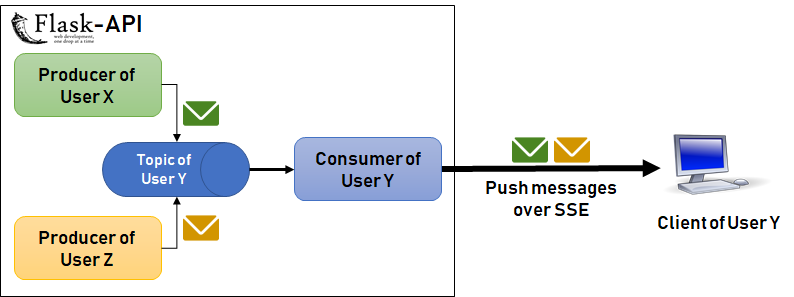
\includegraphics[width=.9\textwidth]{images/SSE-kafkaMessages}
	\caption{Ablauf des Empfangs von Nachrichten über die Apache Kafka Plattform, eigene Darstellung}
	\label{img:SSE-kafkaMessages}
\end{figure}

Die Producer der Chatpartner eines Benutzers produzieren Nachrichten in sein Topic. Der Consumer des Empfängers konsumiert die Nachrichten und der Server sendet die Nachrichten über das Server-Sent-Event an den Client.

In \autoref{lst:flaskPykafkaSSE} ist das Server-Sent-Event dargestellt, das Nachrichten, die von der Kafka Plattform empfangen werden, an den Client übermittelt.

\begin{lstlisting}[language=python, caption={Code des Server-Sent-Events für den Empfang von Nachrichten der Kafka Plattform}, label={lst:flaskPykafkaSSE}]
@app.route('/kafkastream/')
def get_messages():
    client = get_kafka_client()
    def events(user_id):
        global session_dict
        for i in client.topics[session_dict[user_id]['topic']].get_simple_consumer():
            yield 'data: {0}\n\n'.format(i.value.decode())
    return Response(events(current_user.user_id), mimetype="text/event-stream")
\end{lstlisting}

Verbindet sich ein Client auf die \acs{URI} \texttt{193.196.53.24/kafkastream/}, führt die Flask Applikation die Funktion \texttt{get\_messages} aus. Zuerst erzeugt die Methode \texttt{get\_kafka\_client} ein Objekt des Moduls pykafka. Das Objekt verbindet sich automatisch mit dem Kafka-Broker. Anschließend initialisiert die \texttt{Response}-Methode das Server-Sent-Event und ruft die Methode \texttt{events} auf.
Die Operation \texttt{current\_user.user\_id} des Login-Managers gibt die ID des eingeloggten Benutzers zurück, der diese \acs{API}-Route aufruft. Weil die ID für jeden Benutzer unterschiedlich ist, wird damit die Methode \texttt{events} für jeden Benutzer mit unterschiedlichem Argument aufgerufen. Die ID des Benutzers ist Schlüssel des globalen Session-Dictionary. Über die ID und das Session-Dictionary kann das Topic eines bestimmten Benutzers abgefragt werden. Für jeden Benutzer wird über das Topic ein Consumer-Objekt über \texttt{get\_simple\_consumer} erzeugt. Für jeden Benutzer wird ein eigenes Consumer-Objekt erzeugt, dass Nachrichten aus dem Topic des Benutzers konsumiert. Ein Benutzer kann keine Nachrichten empfangen, die nicht für ihn bestimmt sind. Der Generator gibt die eintreffenden Nachrichten zurück, welche dem Client über das Server-Sent-Event zugestellt werden.

Diese Lösung eignet sich auch für den Empfang von Nachrichten über die \acs{XMPP}-basierte Plattform ejabberd. Der sleekxmpp-Client von Python arbeitet mit einer Callback-Methode, die aufgerufen wird, wenn eine neue Nachricht eingetroffen ist. Der Code der Callback-Methode verarbeitet die Nachricht und muss die Nachricht direkt in das Server-Sent-Event weitergeben. Den Server-Push aus der Callback-Methode heraus auszulösen, ist mit den Möglichkeiten von Flask nicht möglich. Das Generator-Objekt muss hierzu von der Callback-Methode befüllt werden, was nicht möglich ist. Ein Generator-Objekt kann nur einmal erstellt werden und produziert solange Werte, bis die Abbruchbedingung zutrifft. Eine Aktualisierung des Generator-Objekts, während es ausgeführt wird, ist nicht möglich. Diesen Entschluss bestätigt die Recherche nach einer Möglichkeit, ein Generator-Objekt zu aktualisieren. Die Empfehlung von Communities wie \glqq stackoverflow.com\grqq\ ist ein Generator-Objekt neu zu erzeugen, statt es zu aktualisieren \cite{resetGeneratorObjectPython}. Zusätzlich ist fraglich, was eine geeignete Abbruchbedingung innerhalb des Generator-Objekts ist, denn der Empfang der Nachricht lässt sich nur über die Callback-Methode realisieren. Sleekxmpp bietet keine Schnittstelle für Entwickler, um auf eine Queue oder Liste, in der die Nachrichten zwischengespeichert werden, zuzugreifen.

Eine geeignete Lösung ist, Redis als Zwischenspeicher von Nachrichten einzusetzen. Redis ist eine In-Memory Datenbank und ist Open-Source. Eine In-Memory Datenbank speichert Daten im nicht persistenten Speicher (\acs{RAM}). Redis kann als Cache, High-Performance Datenbank und als Message-Broker verwendet werden.\cite{redisDocumentation}

Für die Lösung mit dem sleekxmpp-Client wird Redis als Message-Broker eingesetzt, der die Nachrichten im \acs{RAM} zwischenspeichert. Redis arbeitet nach dem in \autoref{img:PublishSubscribeTanenbaum} auf Seite \pageref{img:PublishSubscribeTanenbaum} vorgestellten Publish-Subscribe-Prinzip, mit dem Unterschied, dass der Datenraum nicht persistent ist. Im Zusammenhang mit Redis und dem Publish-Subscribe-Prinzip gibt es drei wichtige Fachbegriffe, die häufig verwendet werden: Publisher, Subscriber und Channel. Publisher produzieren Nachrichten in einen Channel von Redis, aus denen Subscriber die Nachrichten lesen können. Die Voraussetzung dafür ist, dass der Subscriber sich bei Redis für den Channel registriert.

\autoref{img:RedisFunction} verdeutlicht die Funktion des Publish-Subscribe-Prinzips von Redis nach \cite{redisDocumentation}.

\begin{figure}[h]
	\centering
	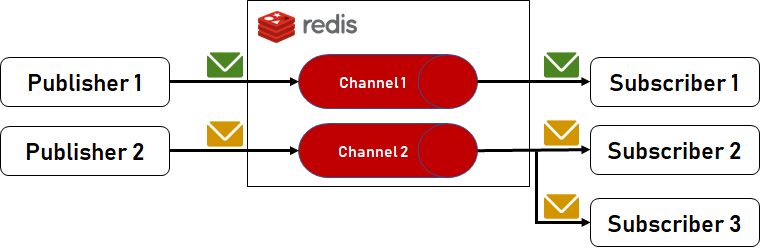
\includegraphics[width=\textwidth]{images/RedisFunction}
	\caption{Funktion des Publish-Subscribe-Prinzips von Redis, eigene Darstellung}
	\label{img:RedisFunction}
\end{figure}

Mehrere Publisher können in einen Channel Nachrichten schreiben und umgekehrt können mehrere Subscriber Nachrichten aus einem Channel lesen. Ein Channel ist die logische Verbindung zwischen Publisher und Subscriber, über den die Nachrichten ausgetauscht werden.\cite{redisDocumentation}

Flask unterstützt das Python Modul redis-py, mit dem Publish- und Subscribe-Operationen in die In-Memory Datenbank veranlasst werden können.

\autoref{lst:prepareFlaskForRedis} zeigt, wie eine In-Memory Datenbank mit Python erstellt werden kann und die Benutzung von Redis vorbereitet wird.

\begin{lstlisting}[language=python, caption={Code für die Einbindung von Redis in die Flask Applikation}, label={lst:prepareFlaskForRedis}]
import redis
#more imports ...

app = Flask(__name__)
red = redis.StrictRedis(decode_responses=True)
#more code ...
\end{lstlisting}

Nach dem Import des Moduls im Code der Flask Applikation muss eine StrictRedis-Instanz erzeugt werden. Über diese Instanz, in \autoref{lst:prepareFlaskForRedis} \glqq redis\grqq\ genannt, können Nachrichten in Channels produziert werden oder aus einem Channel gelesen werden.

\pagebreak

Wichtige Operationen:

\begin{description}
\item[red.publish(<channel>, <message>)] Eine Nachricht in einen bestimmten Channel hineinschreiben (Publish-Operation).
\item[red.subscribe(<channel>)] Einen Channel abonnieren (Subscribe-Operation).
\item[red.listen()] Nachrichten aus dem abonnierten Channel lesen.
\end{description}

In \autoref{img:RedisSleekxmppMessages} ist der logische Ablauf bei der Zustellung der Nachrichten über das Server-Sent-Event und Redis abgebildet.

\begin{figure}[h]
	\centering
	\includegraphics[width=\textwidth]{images/RedisSleekxmppMessages}
	\caption{Empfang von Nachrichten über das Server-Sent-Event mit Redis, eigene Darstellung}
	\label{img:RedisSleekxmppMessages}
\end{figure}

Die Sleekxmpp-Clients der Sender versenden die Nachrichten an ejabberd über \acs{XMPP}. Die Sleekxmpp-Clients der Empfänger warten auf eingehende Nachrichten vom ejabberd-Server. Trifft eine Nachricht ein, produziert die Callback-Methode des Sleekxmpp-Objekts die Nachricht in den Channel des Empfängers. Diese Operation ist die Publish-Operation. Beim Login eines Benutzers am \acs{IMS} wird eine Channel-ID zufällig erzeugt und dem Benutzer im Session-Dictionary zugewiesen. Auf diese Weise ist die Zuordnung von einem Benutzer zu seinem Channel nach dem Login eindeutig gegeben. Auf diese Funktion wird im Detail nicht genauer eingegangen. Die Beschreibung hat keinen Mehrwert für die Lösung des Empfangs einer Nachricht. Die Flask Applikaion liest über die Subscribe-Operation die Nachrichten aus dem Channel des Benutzers und stellt diesen die Nachrichten über ein Server-Sent-Event zu.

\pagebreak

Der Code für das Server-Sent-Event ist in \autoref{lst:flaskSleekxmppSSE} dargestellt.

\begin{lstlisting}[language=python, caption={Code des Server-Sent-Events für den Empfang von Nachrichten über ejabberd}, label={lst:flaskSleekxmppSSE}]
@app.route('/stream')
def stream():
    def event_stream(user_id):
        pubsub = red.pubsub()
        global session_dict
        stream_id = session_dict[user_id]["stream_id"]
        pubsub.subscribe(stream_id)
        for message in pubsub.listen():
            yield 'data: %s\n\n' % message['data']
    return Response(event_stream(current_user.user_id), mimetype="text/event-stream", status=200)
\end{lstlisting}

Verbindet sich ein Client auf die \acs{URI} \texttt{http://193.196.53.24/stream}, führt die Flask Applikation die Methode \texttt{stream} aus. Die Methode \texttt{Respone} des Flask-Moduls ruft für jeden Benutzer die Methode \texttt{event\_stream} auf, die Daten für das Server-Sent-Event produziert. Genau wie in \autoref{lst:flaskPykafkaSSE}, sorgt die Operation \texttt{current\_user.user\_id} dafür, dass sich das Argument der Methode \texttt{event\_stream} je nach Benutzer unterscheidet. Die Benutzer-ID wird dafür verwendet, um für jeden Benutzer die Channel-ID aus dem Session-Dictionary auszulesen. In \autoref{lst:flaskSleekxmppSSE} ist die Channel-ID \glqq stream\_id\grqq\ genannt. Anschließend werden über den Subscribe-Mechanismus die Nachrichten aus dem Channel gelesen und der Generator produziert die Nachrichten in den Event-Stream. Der Client erhält die Nachrichten über den Event-Stream.

Mit Server-Sent-Events werden die Nachrichten automatisch dem Client übermittelt. Wird die Verbindung unterbrochen, verbindet sich der Client-Code automatisch erneut mit dem Server-Sent-Event. Die Lösung macht den Empfang von Nachrichten direkt am Client oder in einem Web Frontend möglich.

\section{Hinzufügen von Benutzern als Kontakte}

Dieser Abschnitt befasst sich mit der Implementierung einer Funktion, die es Benutzern ermöglicht, andere Benutzer als Kontakt hinzuzufügen. Die Funktionalität in einem \acs{IMS} ist wichtig, weil sonst keine Kommunikation mit Benutzern stattfinden kann. Ein Benutzer soll einen Kontakt selbstständig hinzufügen kennen, wenn er den Benutzernamen des zukünftigen Chatpartners kennt.

Ein Benutzer kann einen anderen Benutzer zu seinen Kontakten hinzufügen, wenn sein Client eine \acs{HTTP}-Post Anfrage an die \acs{API}-Route \texttt{http://193.196.53.24/add\_contact} sendet.

Im Anhang in \autoref{img:umlAddContactStudienarbeit} ist die Anwendungslogik in einem \acs{UML}-Aktivitätsdiagramm dargestellt. Die \acs{API} führt die darin dargestellten Abläufe durch, wenn ein Client die \acs{API} beauftragt, einen Kontakt hinzuzufügen. Im ersten Schritt wird überprüft, ob der Benutzer am \acs{IMS} angemeldet ist. Falls das nicht der Fall ist, sendet die \acs{API} dem Client eine Fehlermeldung im Datenaustauschformat \acs{JSON}. Falls der Benutzer angemeldet ist, überprüft die \acs{API}, ob die im \acs{HTTP}-Payload vorhandenen Daten valide sind. Der Name des Benutzers, der als Kontakt hinzugefügt werden soll, und die benutzte Plattform müssen im \acs{JSON}-Payload enthalten sein. Die \acs{API} überprüft, ob der Benutzername aus dem Payload in der Datenbank existiert und sendet dem Client, falls das nicht der Fall ist, eine Fehlermeldung. Zusätzlich wird sichergestellt, dass ein Benutzer sich nicht selbst als Chatpartner hinzufügen kann. Sind die Daten valide, entscheidet die \acs{API} anhand des Wertes im Payload, für welche Plattform der Benutzer hinzugefügt werden soll. Zum Beispiel kann ein Benutzer, der für die Plattform ejabberd angemeldet ist, einen anderen Benutzer als Kontakt nur in seine Kontaktliste der ejabberd-Plattform hinzufügen, aber nicht für die Plattform Kafka. Umgekehrt wenn er an der Plattform Kafka angemeldet ist, kann er nur Kontakte für die Plattform Kafka hinzufügen, aber nicht für ejabberd. Der Mehrwert ist, dass so die Entwicklung weniger aufwendig ist. Anschließend wird der Kontakt für die entsprechende Plattform hinzugefügt und die Benutzer können sich gegenseitig Nachrichten schreiben.

Beim Hinzufügen eines Kontakts auf der Plattform ejabberd, benutzt die \acs{API} den Sleekxmpp-Client von Python. Hierfür verwendet dieser das \acs{XMPP}-Protokoll, um den ejabberd-Server die Änderung in seiner Kontaktliste mitzuteilen. Der Kontakt kann über die Methode \texttt{update\_roster} des Moduls Sleekxmpp hinzugefügt werden.

\autoref{lst:sleekxmppUpdateContacts} zeigt den Ausschnitt des Codes der \acs{API}-Route, der die Kontaktliste über den Sleekxmpp-Client aktualisiert.

\begin{lstlisting}[language=python, caption={Code für das Hinzufügen eines Kontakts über \acs{XMPP}}, label={lst:sleekxmppUpdateContacts}]
# error handling code
if JSON_Data.get("requested_platform") == "xmpp":
    session_dict[current_user.user_id]["xmpp_object"].update_roster(f'{user_name}@{config["ejabberd_domain"]}', name=user_name)
    # send successfull message or handle errors
\end{lstlisting}

In \texttt{JSON\_Data} befinden sich die Daten des \acs{JSON}-Payloads vom Client. Ist \texttt{requested\_platform} im Payload auf \texttt{xmpp} gesetzt, wird der neue Chatpartner über den Sleekxmpp-Client zur Kontaktliste des Benutzers hinzugefügt. Die Methode wird über das Sleekxmpp-Objekt des Benutzers aus dem Session-Dictionary aufgerufen. Denn das Sleekxmpp-Objekt verwaltet über den ejabberd-Server die Kontaktliste des Benutzers. Die Methode erhält als Argumente die Jabber-ID und den Namen des Benutzers, der hinzugefügt werden soll. Zum Schluss sendet die \acs{API} ein \acs{JSON}-Objekt an den Client zurück, das den Ausgang der Operation enthält.

\textbf{Bemerkung:} Mit dem Modul Sleekxmpp lässt sich nur die eigene Kontaktliste aktualisieren. Umgekehrt hat der neu hinzugefügte Kontakt nicht den Benutzer, der ihn hinzugefügt hat, in seiner Kontaktliste. Eine Möglichkeit die Kontaktliste des anderen Benutzers mit zu aktualisieren ist mit der \acs{XMPP}-Erweiterung \texttt{XEP-0321} möglich. Für mehr Informationen siehe \cite{xep0321remoteRosterMgmt}. Die Erweiterung wird allerdings nicht von Sleekxmpp unterstützt. Auch ist es nicht möglich, das Sleekxmpp des anderen Benutzers aus dem Session-Dictionary direkt zu benutzen, um seine Kontaktliste ebenfalls zu aktualisieren. Der Benutzer muss nicht am System angemeldet sein und deshalb kein Sleekxmpp-Objekt des Benutzers im Session-Dictionary vorhanden sein. Auch kann kein Objekt neu erzeugt werden, denn dafür ist ein Passwort notwendig. Das Passwort ist aber im \acs{IMS} nicht im Klartext gespeichert.

Eine Lösung ist, das Hinzufügen des anderen Benutzers zu ignorieren. Durch den Chatverlauf kann der andere Benutzer ihm immer antworten und vergangene Nachrichten sehen. Diese Lösung wird in der Studienarbeit verwendet.

Um einen Kontakt für die Plattform Kafka hinzuzufügen, wird die \autoref{tab:tableContacts} benötigt, in der die Kontakte von Benutzern der Apache Kafka Plattform gespeichert werden. Fügt ein Benutzer einen Kontakt hinzu, muss die \acs{API} zwei Zeilen in die Tabelle aus \autoref{tab:tableContacts} eintragen.

\autoref{tab:tableAddContactKafka} zeigt ein Beispiel, wenn Benutzer mit der ID 41 den Benutzer mit der ID 32 als Kontakt hinzufügt.

\begin{table}[h]
\centering
\caption{Eintrag in die Tabelle contacts für das Hinzufügen eines Kontakts der Plattform Apache Kafka}
\begin{tabular}{|l|l|}
\hline
\textbf{user\_id} &  \textbf{peer\_id} \\
\hline
... & ... \\
\hline
41 & 32 \\
\hline
32 & 41 \\
\hline
... & ... \\
\hline
\end{tabular}
\label{tab:tableAddContactKafka}
\end{table}

Dieser Mechanismus stellt sicher, dass sich beide Benutzer gegenseitig als Kontakt hinzufügen und keine Fehler entstehen, wenn ein Benutzer dem Anderen eine Nachricht sendet.

In \autoref{lst:kafkaUpdateContacts} ist ein Ausschnitts des Codes der \acs{API}-Route dargestellt, der den Benutzer als Kontakt für die Plattform Apache Kafka hinzufügt. Das Listing lässt sich als Fortsetzung von \autoref{lst:sleekxmppUpdateContacts} betrachten.

\begin{lstlisting}[language=python, caption={Code für das Hinzufügen eines Kontakts der Plattform Kafka}, label={lst:kafkaUpdateContacts}]
# error handling code
# Fortsetzung von Listing 5.53.
elif JSON_Data.get("requested_platform") == "kafka":
    sql = # SQL-Befehl für das Hinzufügen in die Datenbank als String
    db.session.execute(sql, {'user_id': current_user.user_id, 'username': user_name})
    db.session.commit()
    # send successfull message or handle errors
\end{lstlisting}

Der SQL-Befehl wird in einer Variablen als Zeichensatz vorbereitet. Die Methode \texttt{execute} fügt die Einträge des Dictionary in das SQL-Statement ein. Die Operation \texttt{current\_user.user\_id} gibt die Benutzer-ID des Benutzers zurück, der am \acs{IMS} angemeldet ist und die \acs{API}-Route aufruft. Anhand der Benutzer-ID des Aufrufers und dem Namen des Benutzers, den der Aufrufer als Kontakt hinzufügen möchte, fügt die Methode \texttt{execute} die beiden Zeilen in die Tabelle der Datenbank ein (siehe \autoref{tab:tableAddContactKafka}).

Der Mehrwert für die Entwicklung des \acs{IMS} ist, dass Benutzer Kontakte hinzufügen können und die Chatfunktionalitäten um weitere typische Funktionen eines \acs{IMS} erweitert werden.

\pagebreak

\chapter{Entwicklung des Frontends für den XMPP-Client}
\label{sec:FrontendXMPP}
Einleitend geht der \autoref{sec:GuiPython} auf die Möglichkeiten einer grafischen Benutzeroberfläche mit Python ein. Mit dem Resultat der Entscheidungsmatrizen aus \autoref{tab:EntscheidungsmatrixFrameworkart} und \autoref{tab:EntscheidungsmatrixWebFramework} wird das Web Frontend mithilfe der in \autoref{sec:HTMLCSSJS} erläuterten Werkzeuge einer Webentwicklung realisiert. In diesem Zusammenhang werden im Folgenden alle relevanten HTML- und JavaScript-Dateien analysiert und detailliert erläutert. 

Vorab ist der Begriff des XMPP-Clients zu definieren. Mit der Entwicklung eines Chatsystem auf Basis von XMPP wird das Ziel verfolgt ejabberd als Messaging-System und XMPP als Kommunikationssprache zu nutzen. Dafür wird sowohl ein Server als auch ein Client benötigt. Mit der Projektumsetzung auf der Web-Plattform kann der Client verschieden definiert werden. Nach Günter Pomaska kann der Client sowohl die Hardware, als auch die Software darstellen.\cite{pomaska2012webseiten}. Demnach handelt es sich bei dem XMPP-Client um die Software bzw. den Browser welcher über XMPP mit dem Server kommuniziert.

\section{Das Prinzip der Webseiten-Programmierung}
\label{WebsiteProgramming}
Bei der Entwicklung eines Frontends für eine Web-Applikation sind wichtige Bestandteile zu beachten. Diese bilden den Kern des Unterabschnitts. Wie der Einführung zu entnehmen ist bilden die Werkzeuge aus \autoref{sec:HTMLCSSJS} den Kern der Webseiten-Programmierung. Diese werden nach Günter Pomaska als \glqq Sprachen im Web\grqq\ bezeichnet. Zu den Sprachen kommt die Webseite als weiteres Bestandteil hinzu. Für die Entwicklung des Frontends ist die Kenntnis über das Ausliefern von Webseiten relevant. Dafür kann die \autoref{img:WebseiteAnforderung} betrachtet werden.
\begin{figure}[h]
	\centering
	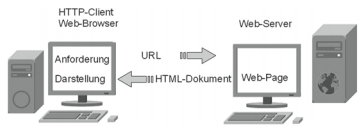
\includegraphics[scale=2.1]{images/WebseiteAnfordern}
	\caption{Das Anfordern einer Webseite eine Clients, \cite{pomaska2012webseiten}}
	\label{img:WebseiteAnforderung}
\end{figure}
Mithilfe einer URL kann der Client eine Webseite vom Web-Server anfordern. Nach der Datenübertragung wird die Seite vom Browser dargestellt. Bezogen auf dieses Funktionsprinzip können die Inhalte nicht ohne eine erneute Anforderung verändert werden. Daher werden HTML-Dokumente als statische Dateien bezeichnet. Wird eine client-seitige Dynamik mithilfe von Javascript und dem \ac{DOM} integriert, können die Webinhalte client-seitig ohne Neuanforderung verändert werden. Eine Variante, welche heutzutage fester Bestandteil der Webseiten-Programmierung ist. \cite{pomaska2012webseiten}
Bei der Implementierung dynamischer Elemente, wie der Formularüberprüfung auf Seiten des Clients, kann die Verknüpfung zu den Prinzipien hergestellt werden. Außerdem tritt das Konstrukt aus \autoref{img:WebseiteAnforderung} in mehreren Bereichen der Client-Entwicklung auf.

\section{Organisation und Aufbau des Frontends}
\label{AufbauFrontendXMPP}
Für die Entwicklung eines Web-Frontends bildet eine Rahmenstruktur die Basis. Hierbei handelt es sich um den Webauftritt durch die Verknüpfung mehrerer HTML-Dateien.\cite{buhler2017html5}
Um auf den \ac{HTML}-Aufbau der Webseiten einzugehen ist das Verständnis über die Struktur und die Verknüpfung der Einzelseiten relevant. Für diese Verknüpfungen können die nachfolgenden Abbildungen betrachtet werden.
\begin{figure}[h]
	\begin{minipage}[c]{.38\textwidth}
		\includegraphics[scale=0.45]{images/HTMLDateienOrdner}
		\caption{HTML-Dateien, eigene Darstellung}
		\label{img:HTMLDateienOrdner}
	\end{minipage}
	\hspace{0.05\linewidth}% Abstand zwischen Bilder
	\begin{minipage}[c]{.5\textwidth}
		\includegraphics[scale=0.5]{images/HTMLDateienAufrufbaum}
		\caption{Interaktionen zwischen den Dateien, eigene Darstellung}
		\label{img:DateinAufrufbaum}
	\end{minipage}
\end{figure}
\autoref{img:HTMLDateienOrdner} zeigt welche HTML-Dateien für die Applikation bzw. für den XMPP-Client relevant sind und wo diese in der Ordnerstruktur zu finden sind. Die Ordnerstruktur hängt mit der Verwendung von Flask zusammen und orientiert sich an dem \autoref{sec:Flask}. Die zweite \autoref{img:DateinAufrufbaum} zeigt wie die Seiten sich gegenseitig benötigen. Hierbei handelt es sich nicht um Referenzen innerhalb des Source-Codes, sondern um die Aufrufstruktur für den Nutzer. Mit der \texttt{index.html}, dargestellt in kursiver Schrift, wird angedeutet, dass kein Nutzer diese Seite ausgeliefert bekommt. Dieses \ac{HTML}-Dokument dient lediglich als Basis. Die weiteren Dateien erben den Inhalt der index.html, was die UML-Notation andeuten soll. Auf der zweiten Ebene hat der Nutzer die Möglichkeit zwischen den Dateien, welche hinter einem API-Endpunkt liegen, zu wechseln, je nach Verwendung. Mit dem Verständnis über die Beziehungen der Dateien wird im Folgenden auf den \ac{HTML}-Aufbau der einzelnen HTML-Dokumenten eingegangen.

\section{Vererbung von Webseiten mithilfe von Flask}
\label{subsec:TemplateInheritance}
Flask als microframework bietet zahlreiche Möglichkeiten. Aus \autoref{sec:Flask} ist bekannt, dass Flask mehrere Komponenten beinhaltet. Eines kann als Jinja identifiziert werden, welches unter anderem als Template-Bibliothek bezeichnet wird. Wie dem vorherigen Abschnitt zu entnehmen ist, handelt es sich bei dem Konzept des Frontends um die Vererbung von HTML-Elementen. Ein Konzept, welche durch Jinja ermöglicht wird.

Die offizielle Seite von Flask bezeichnet das Vererben von HTML-Vorlagen als mächtigstes Tool von Jinja. Die Vererbung erlaubt das Konstruieren eines Rahmens für den gesamten Webauftritt. Um dieses Prinzip zu verwenden werden mindestens 2 HTML-Seiten benötigt. In einem ersten Schritt wird das sogenannte \glqq Base Template\grqq\ definiert. Diese Seite verkörpert den Rahmen, wobei es alle Elemente, welche dauerhaft benötigt werden, implementiert. Ein Beispiel für die Grundseite ist im \autoref{lst:BaseTemplate} dargestellt.
\begin{lstlisting}[language=HTML,caption=Beispiel einer Grundseite für das Vererbungsprinzip,label={lst:BaseTemplate}]
<!doctype html>
<html>
	<head>
		
		<link rel="stylesheet" href="">
		<title> - My Webpage</title>
		
	</head>
	<body>
		<div id="content"></div>
		<div id="footer">
			
			
		</div>
	</body>
</html>
\end{lstlisting}
Das hinzugewonnen Feature ist die Unterteilung des Base Templates in Blöcke. Diese werden mit \texttt{\{\% Block X\%\}} eingeleitet. Den Abschluss eine Blocks wird mit \texttt{\{\% endblock \%\}} dargestellt. Ein Block, wie er im \autoref{lst:BaseTemplate} dargestellt ist, wird vom Base Template definiert. Dadurch wird indirekt ein freiere Raum konstruiert, der von dem Kindelement befüllt werden kann ohne Inhalte zu überschreiben. Das Base Template lässt sich laut der Dokumentation als Elternteil bezeichnen. Im weiteren Verlauf bieten die Blöcke die Möglichkeit von Kindelementen überschrieben zu werden. Die Aufgabe eines \glqq Child Templates\grqq\ besteht darin, die leeren Blöcke mit Inhalt zu füllen. Aufschluss darüber wie eine Kindseite das löst, bildet das \autoref{lst:ChildTemplate} ab. Demnach beginnt das HTML-Dokument nicht mit den Standard-Tag \texttt{<!doctype html>}, sondern stellt die Verknüpfung zum Base Template her. In dem Fall stellt das \texttt{extends} ein Keyword dar, wodurch alle HTML-Elemente der Elternseite übernommen werden. Das umfasst die HTML-Tags und was damit einhergeht. Außerdem werden die Blöcke als eine Art Rahmen übernommen.
\begin{lstlisting}[language=HTML,caption=Beispiel für Kindseite beim Vererbungsprinzip von Jinja,label={lst:ChildTemplate}]

Index

	{{ super() }}
	<style type="text/css">
		.important { color: #336699; }
	</style>


	<h1>Index</h1>
	<p class="important">
	Welcome on my awesome homepage.

\end{lstlisting}
Um die Blöcke mit Inhalt zu füllen replizieren die Kindseiten den Blocknamen. Anschließend können die HTML-Tags und Attribute definiert werden. Im Folgenden liegt das Augenmerk auf Zeile 4 von \autoref{lst:ChildTemplate}. Wird der Block von einem Kindelement mit Inhalt befüllt, würden die Blockinhalte des Elternelements überschrieben werden. Um dieses Vorgehen zu verhindern kann mithilfe von \texttt{\{\{ super() \}\}} die Blockinhalte des Base Templates übernommen werden. Dieses Prinzip der Vererbung finden Verwendung bei der Entwicklung der index.html. \cite{FlaskTempInherDoc}

\section{Strukturaufbau der Webseiten}
\label{subsec:StrukturaufbauWebseiten}
Aus dem aktuellen Kenntnisstand geht hervor, dass ein Webauftritt durch mehrere Werkzeuge realisiert werden kann. Mit der Implementierung und Erörterung des Strukturaufbaus wird das HTML-Grundgerüst gebildet. Daher sind die einzelnen Seiten aus \autoref{img:HTMLDateienOrdner} mit den HTML-Elementen der Kern des Abschnittes. Zur Vereinfachung der Darstellung wird auf ausführlichen HTML-Code verzichtet. Ausschließlich wichtige Bestandteile für die Webseite und ihrer Funktion als Teil des XMPP-Clients werden dargestellt. Bei diesen handelt es sich um:
\begin{itemize}
	\item HTML-Tags, welche für den Webauftritt benötigt werden
	\item Klassennamen
	\item Identifikationsnamen
	\item Verschachtelungen je nach Relevanz
\end{itemize}
HTML-Code wird im Folgenden durch Abbildungen erläutert. Ein HTML-Tag bildet demnach eine Box mit schwarzen Rahmen. Dadurch können Verschachtelungen als innere Elemente der äußeren Box dargestellt werden. Füllt sich im Verlauf eine HTML-Box, so werden unrelevante Boxen grau abgebildet.

Eine Struktur als Rahmen der Webseite basiert grundlegend auf die Verwendung von \ac{HTML}. Für die Webseite bedeutet das, dass die Struktur aus div-Boxen und anderen \ac{HTML}-Elementen besteht. Die div-Box kann den Tags, welche in \autoref{sec:HTMLCSSJS} erläutert sind, zugeordnet werden. Das erweitert den Umfang der \ac{HTML}-Tags aus \autoref{sec:HTMLCSSJS} um eine weitere Variante. Grundsätzlich basiert ein Webauftritt auf einer index.html Datei, welche als Ausgangspunkt für den ersten Aufruf eines Nutzers dient. Bezogen auf die Struktur gibt es bei der Web-Entwicklung lediglich Vorschläge für die Umsetzung, dennoch ist das Konzept nach eigenen Anforderungen zu definieren. Demnach kann eine Webseite komplett in der \texttt{index.html} Datei ausgeliefert werden, oder für jede Route, die der Nutzer adressieren kann, wird eine neue \ac{HTML}-Datei ausgeliefert. Im Rahmen der Studienarbeit wird das zweite Konzept verfolgt, weshalb die index.html Datei lediglich als Basis für eine einheitliche Struktur dient. Dieses Konzept ist in der \autoref{img:DateinAufrufbaum} dargestellt und im \autoref{subsec:TemplateInheritance} beschrieben. Außerdem ist daraus ersichtlich, dass die index.html nicht direkt ausgeliefert wird. Wie die nachfolgende \autoref{img:index-struktur} zeigt, bildet der nav-Tag das Konstrukt, welches der Hauptbestandteil der index-Seite und damit dem Base Template darstellt.
\begin{figure}[h]
	\centering
	\includegraphics[width=\linewidth]{images/indexbody}
	\caption{Navigationsleiste innerhalb des Base Templates, eigene Darstellung}
	\label{img:index-struktur}
\end{figure}
Der nav-Tag wird unter der Verwendung einer Navigationsleiste in HTML5 benutzt. Mit der Verwendung des speziellen Klassenamens wird auf Bootstrap referenziert. Welche Rolle der Klassenname bei Bootstrap hat, ist Bestandteil von \autoref{sec:Bootstrap}. Das Konstrukt ist Teil der index-Datei, um eine einheitliche Navigationsleiste für jede weitere Webseite zu definieren. Des Weiteren sind dieser Leiste HTML-Elemente zuzuordnen. Der strukturelle Aufbau mit den Ergänzung an dem Basis-Konstrukt ist in der folgenden \autoref{img:index-strukturInhalt} dargestellt.
\begin{figure}[h]
	\centering
	\includegraphics[width=\linewidth]{images/indexbodyInhalt}
	\caption{Erweiterung der Navigationsleiste um weitere HTML-Elemente, eigene Darstellung}
	\label{img:index-strukturInhalt}
\end{figure}\\
Die Erweiterungen beinhalten zwei i-Tags, welche Icons darstellen bzw. hervorheben sollen. Interessant an diesen Tags ist der Klassenname. Aufgrund der Verwendung von Bootstrap können spezielle Klassennamen angewendet werden, um auf Styles zu referenzieren. Das Gleiche gilt für Icons. Nur besteht dadurch eine Referenz auf die \texttt{fontawesome.min.css} Datei aus \autoref{img:BootstrapStructer}. Der a-Tag definiert eine Referenz in Form eines Hyperlinks, welcher zu einer angegebenen Seite verzweigen kann. Grundidee ist hierbei die Verzweigung des Logos auf die index-Seite bzw. auf die Webseite, die der Nutzer als home-Seite betrachten soll. Die div-Box als letztes Element der Index-Seite beinhaltet weitere Elemente, die keine Relevanz für den Strukturaufbau der Webseite darstellen. Diesem Element sind überwiegend weitere Links und Textfelder zugeordnet, wie es der \autoref{img:Navbar} zu entnehmen ist. Den \ac{HTML}-Elementen kann mithilfe von \ac{CSS} gestalterische Aspekte verliehen werden. Diese Aufgabe kann das unter \autoref{sec:Bootstrap} vorgestellte Framework namens Bootstrap übernehmen. Mit kleinen Ergänzungen zur den vorgefertigten CSS-Elementen von Bootstrap stellt die \autoref{img:Navbar} die vollständige index-Seite dar, welche ausschließlich zur Vererbung dient. 
\begin{figure}[h]
	\centering
	\includegraphics[width=\linewidth]{images/indexHTML&CSS}
	\caption{Webbrowserdarstellung der Index-Seite, eigene Darstellung}
	\label{img:Navbar}
\end{figure}\\
Aufbauend auf der Index-Seite können alle weiteren Webseiten die Navigationsleiste über die index.html Datei erben, wie es das Konzept aus \autoref{img:DateinAufrufbaum} darstellt. Hierfür wird die Vorgehensweise aus \autoref{subsec:TemplateInheritance} verwendet. Dadurch kann eine durchgängige Struktur beibehalten werden. Die Index-Seite bildet daher keine Möglichkeit durch einen Nutzer direkt adressiert zu werden. Die erste Anlaufstelle eines unangemeldeten Nutzers wird durch die Login-Seite abgebildet. Unabhängig von der Navigationsleiste bietet die \texttt{login.html} Datei ein Formular für den Anmeldevorgang.

\pagebreak

Mit Hilfe von Bootstrap wird die Basis-Struktur durch div-Boxen und Klassennamen definiert, wie sie der folgenden \autoref{img:BasisStrukturLogin} zu entnehmen sind.
\begin{figure}[h]
	\centering
	\includegraphics[width=\linewidth]{images/loginBasisStruktur}
	\caption{Basis-Struktur der login-Seite, eigene Darstellung}
	\label{img:BasisStrukturLogin}
\end{figure}
Basierend auf diesem Aufbau bildet die Klasse \texttt{d-flex justify-content-center} die Möglichkeit weitere div-Boxen flexibel anzuordnen. Eine Variante wie sie in \autoref{sec:HTMLCSSJS} unter \ac{CSS} erläutert wird. Die \autoref{img:BasisStrukturLogin} bildet noch kein Formular der Login-Seit ab, sondern lediglich einen Container für eine korrekte Anordnung. Im Folgenden wird der div-Box mit der Klasse \texttt{content-section pt-5 pl-5} ein form-Tag hinzugefügt, um in Kooperation mit Bootstrap ein Formular, bezogen auf die Anmeldung, zu konstruieren.
\begin{figure}[h]
	\centering
	\includegraphics[scale=0.55]{images/loginBasisStruktur&FormContainer}
	\caption{Integration des Formular-Tags in die Login-Basisstruktur, eigene Darstellung}
	\label{img:BasisStrukturLoginUnd Formular}
\end{figure}\\
Die Design-Elemente werden über der Bootstrap-Datei dem Formular mitgegeben. Der strukturelle Aufbau der Login-Seite ist damit vollendet. Für das Formular werden dem form-Container Textfelder, Buttons und ähnliches hinzugefügt, welche das Formular gestalterisch vervollständigen.

\pagebreak

Diese Elemente sind in der \autoref{img:LoginSeiteVollständig} dargestellt. Außerdem bildet die \autoref{img:LoginSeiteVollständig} die vollständige Login-Seite ab, wobei dieser Webseite eine weitere div-Box zugeteilt werden kann, welche für die Struktur keine Relevanz darstellt und daher nicht aufgeführt ist.
\begin{figure}[h]
	\centering
	\includegraphics[width=\linewidth]{images/loginSeiteFertig}
	\caption{Vollständige Login-Seite, eigene Darstellung}
	\label{img:LoginSeiteVollständig}
\end{figure}
Die Registrierungs-Seite ist ähnlich zur Login-Seite. Aus diesem Grund wird die Registrierungs-Seite nicht ausführlich erklärt, sondern lediglich die HTML-Inhalte und das Design dargestellt. Einziges unterscheidendes Merkmal zur Login-Seite sind die HTML-Elemente innerhalb des Formulars, welche sich vor allem in der Anzahl unterscheiden. Die folgende \autoref{img:RegisterSeiteVollständig} zeigt sowohl die Struktur als auch die Darstellung für den Nutzer.
\begin{figure}[h]
	\centering
	\includegraphics[width=\linewidth]{images/RegisterPage2}
	\caption{Vollständige Registrierungs-Seite, eigene Darstellung}
	\label{img:RegisterSeiteVollständig}
\end{figure}
Aus der \autoref{img:RegisterSeiteVollständig} sind die erwähnten Unterschiede nicht zu entnehmen, da Sie keinen Einfluss auf die Grundstruktur der Registrierungsseite haben. Ausschließlich bei der Darstellung tieferer Verschachtelungen würden die Unterschiede erkennbar werden.\\ 
Die Hauptseite des Web-Clients wird dem Nutzer durch die \texttt{gochat.html} Datei ausgeliefert. Wie der \autoref{img:DateinAufrufbaum} zu entnehmen ist, kann der Nutzer die Seite von der login.html Seite erreichen. Nach einer Registrierung kann sich ein Benutzer am System anmelden. Die gochat.html Datei beinhaltet den Aufbau des Chats sowie zahlreiche weitere Funktionen welche dem Nutzer nur angeboten werden wenn er angemeldet ist. Ein Securityaspekt, welcher im Backend geregelt wird und kein Bestandteil der HTML-Dokumente ist. Die gochat.html Datei gliedert sich in mehrere HTML-Tags bzw. in mehrere div-Boxen, auf die im einzelnen detaillierter eingegangen wird. Dafür stellt die erste \autoref{img:BasisStruktur1Gochat} eine Art erste Ebene dar, welche die einzelnen Elemente voneinander abgrenzt und eine Struktur für die Teilbereiche bildet.
\begin{figure}[h]
	\centering
	\includegraphics[width=\linewidth]{images/BasisStruktur1Gochat}
	\caption{Strukturierung von gochat.html auf der ersten Ebene, eigene Darstellung}
	\label{img:BasisStruktur1Gochat}
\end{figure}
Die ausgegraute div-Box mit der Klasse \texttt{navbar} wird ausschließlich für die Vollständigkeit mit aufgeführt. Die Klasse ist Teil der index.html und wird von gochat.html geerbt. Dadurch besteht die erste Ebene aus den drei anderen div-Boxen. Die erste div-Box mit der id \texttt{containerMain} deckt den gesamten Viewport der Webseite ab. Dadurch ergibt sich die Möglichkeit innere Container entsprechend des Viewports anzupassen.\\
Ein relevantes Merkmal ist hierbei die Klasse \texttt{row}, welches Bestandteil von Bootstrap ist. Die Klasse kann in mehreren Situationen zum Einsatz kommen. Im Fall von der gochat.html Datei handelt es sich um das Grid-System von Bootstrap. Dieses bietet die Möglichkeit Container bzw. div-Boxen in dem von Bootstrap spezifizierten Grid auszurichten. Dadurch wird dem Anwender die Möglichkeit geboten eine row zu definieren und diese, wie die nachfolgende Abbildung zeigt, in columns zu unterteilen.
\begin{figure}[h]
	\centering
	\includegraphics[scale=0.9]{images/GridSystem}
	\caption{Das Grid System von Bootstrap, \cite{krause2016introducing}}
	\label{img:GridSystem}
\end{figure}
Mit diesem Konzept können die Inhalte problemlos aneinander gereiht bzw. angeordnet werden. \cite{krause2016introducing}\\
Aufgrund dieser Konzeptionierung wird der id \texttt{content-window} die Klasse \texttt{col} zugeordnet. Damit wird gewährleistet, dass sich die div-Box wie eine Spalte anordnet. Die Anordnung kann außerdem über eigene CSS-Styles definiert werden, wie es bei dem Sidepanel der Fall ist. Da die CSS keine detaillierte Auswirkung auf die Struktur hat wird auf diese Styles nicht genaueres eingegangen. Im Folgenden soll das Sidepanel mit seinem Container im Vordergrund stehen. Um die innere Struktur zu definieren sind die Aufgaben bzw. die Anzeigemöglichkeiten des Sidepanels zu definieren. Entsprechend der Aufgaben können Boxen angelegt werden, welche den Inhalt im weiteren Verlauf spezifizieren. Demnach handelt es sich um die folgenden Bestandteile:
\begin{itemize}
	\item Profilanzeige
	\item Suchfunktion innerhalb der eigenen Kontaktliste
	\item Kontaktliste für Einzel- und Gruppenchats
	\item Zusätzliche Optionen
\end{itemize}
Zur Integration in die gochat.html wird für jeden Bestandteil einen eigener Container definiert. Diese werden dem Sidepanel zugeordnet, wie es auf der nachfolgenden \autoref{img:Sidepanel} dargestellt ist.
\begin{figure}[h]
	\centering
	\includegraphics[scale=0.55]{images/BasisStruktur1GochatSidepanel}
	\caption{Erweiterung des Sidepanels um die aufgezählten Bestandteile, eigene Darstellung}
	\label{img:Sidepanel}
\end{figure}
Die eigenständigen Container bietet die Möglichkeit die Elemente getrennt voneinander zu gestalten. Außerdem kann dadurch den Elementen im weiteren Verlauf dynamische Aspekte zugeteilt werden. Damit steht die Struktur des Sidepanels. Den einzelnen Containern können weitere HTML-Elemente zugeordnet werden. Das hat eine tiefere Verschachtelung zur Folge, welche nicht nähers erläutert wird. Lediglich Elemente, die der Nutzer sehen kann sollen kurz dargestellt werden. Für den Container mit der id \texttt{profile} bedeutet das, ein img-Tag für das Profilbild und ein p-Tag für den Namen des Nutzers.
Der \texttt{search}-Box kann ein Inputfield zugeordnet werden, welches dem Nutzer die Möglichkeit bietet Texte einzugeben. \cite{bootstrapOnline}\\
Dem Container, unterhalb der search-Box, kann eine größere Relevanz zugeordnet werden. Grund hierfür ist die Verbindung des Containers mit den Projektanforderungen. Die div-Box mit der Id \texttt{contacts} enthält die Chatpartner des angemeldeten Nutzers.

\pagebreak

Wie die einzelnen Kontakte in den Container integriert werden können, kann der nachfolgenden \autoref{img:SidepanelContacts} entnommen werden. 
\begin{figure}[h]
	\begin{minipage}[c]{.48\textwidth}
		\centering
		\includegraphics[scale=0.52]{images/SidepanelContacts}
		\caption{Darstellung der Kontakte als HTML-Elemente, eigene Darstellung}
		\label{img:SidepanelContacts}
	\end{minipage}
	\hspace{0.04\linewidth}% Abstand zwischen Bilder
	\begin{minipage}[c]{.45\textwidth}
		\centering
		\includegraphics[scale=0.35]{images/KontaktlisteUserview}
		\caption{Darstellung der Kontakte (User View), eigene Darstellung}
		\label{img:KontaktlisteUserview}
	\end{minipage}
\end{figure}
Hierfür kommen die Listen-Elemente von HTML5 zum Einsatz. Das \texttt{ul} definiert die Liste und steht für eine \texttt{unordered list}. Kindelemente des \texttt{ul}-Tags sind die \texttt{li}-Tags. Diese definieren ein Listeneintrag.
Übertragen auf die Funktion handelt es sich bei dem \texttt{ul-Tag} um die Initialisierung einer Liste von Kontakten. Entsprechend symbolisieren die li-Container einen einzelnen Kontakt. Standardmäßig werden Listen unter HTML5 mit Bullets markiert. Diese Eigenschaft kann mithilfe von CSS verhindert werden. Die Klassennamen nehmen Bezug zur den dynamischen und gestalterischen Inhalten. Aus diesem Grund unterscheidet sich ein Klassenname von den anderen. Das Resultat davon, ist die Gestaltung eines einzelnen Kontaktes. Dadurch kann dem Benutzer ein Kontakt als \glqq aktiv\grqq\ bzw. \glqq ausgewählt\grqq\ dargestellt werden. Die Darstellung aus Sicht des Benutzers ist in \autoref{img:KontaktlisteUserview} ersichtlich. \cite{w3schoolsUlTag}\\
Mit der Umsetzung der zusätzlichen Optionen wird der \texttt{bottom-bar} zwei Buttons zugeteilt, welche diese Optionen bereitstellen sollen. Für die div-Box mit der id \texttt{content-window} ist die Vorgehensweise identisch, um alle Aufgabenbereiche, aus den Anforderungen, in der grafischen Benutzeroberfläche abzudecken. Diesem Container müssen daher folgende Bestandteile zugeordnet werden.
\begin{itemize}
	\item Profilanzeige des Chatpartners
	\item Nachrichtenansicht
	\item Möglichkeit eine Nachricht einzugeben (Textfeld)
\end{itemize}
In Abhängigkeit dieser definierten Bestandteile wird jedem ein Container zugeteilt, der die Aufgaben innehalten soll.
\begin{figure}[h]
	\centering
	\includegraphics[scale=0.60]{images/BasisStruktur1GochatContentWindow}
	\caption{Erweiterung des Containers \texttt{content-window} um die aufgezählten Bestandteile, eigene Darstellung}
	\label{img:Content-window}
\end{figure}
Der Klasse \texttt{contact-profil} sind die gleichen HTML-Elemente wie der div-Box \texttt{profile} untergeordnet. Ergänzend dazu ist dem Kontaktprofil des Chatpartners ein Dropdownmenü zugeteilt, welches weitere Optionen bereitstellen soll. Für die Struktur von gochat.html wird dieses Element nicht benötigt. Außerdem ist das Dropdownmenü überwiegend ein CSS-Element, weshalb es kein wichtiger Aspekt in der Struktur darstellt. Der Container mit der Id \texttt{messages-container} bildet lediglich einen Rahmen um die Nachrichten des Chats, weshalb der Container keine besonderen Attribute hat. Dem Container werden ausschließlich weiteren HTML-Elemente zugeteilt. Die Nachrichten entstehen zur Laufzeit und sind daher nur in der Gestaltung zu erläutern. Dafür ist die \autoref{img:ContentWindowChatMessages} zu beachten. Der Abbildung zur Folge hat der Nachrichten-Container eine weitere div-Box sowie Listen-Elemente gekennzeichnet mit dem \texttt{ul} und \texttt{li}-Tag. Übertragen auf die Darstellung der Nachrichten aus \autoref{img:GochatUserview} bilden die Listeneintrag eine einzelne Nachricht. Die Nachrichten werden entsprechend der unterschiedlichen Klassennamen identifiziert. Der \texttt{li}-Tag mit der Klasse \texttt{clearfix} symbolisiert die empfangenen Nachrichten.
\begin{figure}[h]
	\centering
	\includegraphics[scale=0.45]{images/ContentWindowChatMessages}
	\caption{HTML-Ansicht der Nachrichten, eigene Darstellung}
	\label{img:ContentWindowChatMessages}
\end{figure}
Demzufolge steht der leere li-Tag für die gesendeten Nachrichten. Für die detaillierte Darstellung, werden weitere HTML-Elemente innerhalb der Listeneinträge benötigt. Da diese keinen Einfluss auf den strukturellen Aufbau haben, sind sie zu vernachlässigen.\\
Das Hauptmerkmal der Klasse \texttt{input-group} ist das Textfeld und der Button, welches es innehat. Dadurch wird dem Nutzer gewährleistet seine Nachrichten einzugeben und über ein Button zu senden. Weitere HTML-Elemente spielen in der Struktur keine Rolle und sind daher nicht weiters aufgeführt. Alle Elemente, welche die Struktur der gochat.html Datei beschreiben sind in der \autoref{img:Content-window} aufgeführt. Unter der Verwendung von Bootstrap und eigenen Styles zeigt die \autoref{img:GochatUserview} die Hauptseite aus der Sicht des Benutzers.
\begin{figure}[h]
	\centering
	\includegraphics[scale=0.4]{images/GochatUserAnsicht}
	\caption{gochat.html aus Sicht des Nutzers, eigene Darstellung}
	\label{img:GochatUserview}
\end{figure}
Mit der fertigen Struktur von gochat.html sind alle Webseiten, die der Webserver ausliefert, im Detail erörtert. Das Erscheinungsbild, wie es bspw. in \autoref{img:GochatUserview} dargestellt ist entsteht hauptsächlich unter der Verwendung von \ac{CSS}. Diese Details werden aufgrund der Redundanzen und der Ähnlichkeit zu den Beispielen aus \autoref{sec:HTMLCSSJS} nicht nähers erläutert und können dem Source-Code entnommen werden. Eine größere Relevanz spielen die dynamischen Elemente, welche das Nutzerverhalten direkt beeinflussen können. Aus diesem Grund wird der JavaScript Code mit Bezug zur jeweiligen HTML-Datei detaillierter erläutert.
\pagebreak

\section{Integration dynamischer Elemente in die Webseiten}
\label{subsubsec:DynamischeElementeWebseiten}
Der XMPP-Client bzw. die Webseiten benötigen für eine korrekte Ausführung JavaScript. Dadurch können Vorteile genutzt werden, welche Bestandteil im \autoref{sec:HTMLCSSJS} sind. Im Falle des XMPP-Clients bietet JavaScript die Möglichkeit HTML-Elemente zur Laufzeit zu verändern. Eine Veränderung der Styles ist ebenso möglich. Wie JavaScript in den einzelnen Webseiten verwendet wird und was für ein Nutzen es bietet, soll nachfolgende erläutert werden. Die Vorgehensweise orientiert sich an dem vorherigen Abschnitt. Grund hierfür ist die Auswirkung eines JavaScript-Codes auf ein einzelnes \ac{HTML}-Dokument, weshalb die jeweilige Datei mit dem entsprechenden Codesnippet im Vordergrund steht.

Den Anfang stellt die \texttt{index.html} Datei dar. Da die Seite nicht direkt adressiert wird, benötigt die Datei als Basisseite keine dynamischen Elemente. Aufgrund des Konzeptes der Vererbung, aus \autoref{subsec:TemplateInheritance}, können statische Dateien, welche sowohl von Bootstrap als auch von anderen Frameworks benötigt werden, in dem Header mitangegeben werden. 
\begin{lstlisting}[language=HTML,caption=Listing der eingebundenen JS-Dateien im Header der index.html,label={lst:HeaderWithJS}]
<head>
<script src="{{url_for('static',filename='js/jquery-3.4.1.min.js')}}"></script>
<script src="{{url_for('static',filename='js/emojionearea.min.js')}}"></script>
<script src="{{url_for('static',filename='js/bootstrap.min.js')}}"></script>
</head>
\end{lstlisting}
Das \autoref{lst:HeaderWithJS} stellt dar, welche statische Dateien, die lokal auf dem Server liegen, über den relativen Pfad eingebunden werden. Dabei handelt es sich lediglich um ein Ausschnitt ausgewählter Dateien, die in direkter Beziehung zur ihrem Framework liegen. Während jQuery und Bootstrap eindeutig zu identifizieren sind, handelt es sich bei \texttt{emojionearea.min.js} um eine JavaScript-Datei, welche die Realisierung von Emojis ermöglicht. Eine detaillierte Erklärung der \ac{JS}-Dateien, welche als Framework fungieren, sind nicht Bestandteil der Studienarbeit.\\
Mit der \texttt{Login-Seite} entstehen die ersten dynamischen Elemente, welche in der JavaScript-Datei namens \texttt{loginjs.js} implementiert sind. Für einen Überblick sind die Aufgabenbereiche, die mithilfe von \ac{JS} gelöst werden können, zu definieren.
\begin{itemize}
	\item Überprüfen des Loginformulars auf eine Eingabe
	\item Überprüfen der Logindaten auf Korrektheit
	\item Rückmeldungen an den Benutzer
\end{itemize}
Um den Server zu entlasten sind vor allem die Formularfelder clientseitig zu überprüfen. Damit ist vor allem die Überprüfung von leeren Feldern gemeint. Außerdem kann mithilfe von JavaScript die Dateninhalte, nach der Überprüfung, dem Server übermittelt werden. Wie es bei JavaScript üblich ist, referenzieren viele Funktionen auf \ac{HTML}-Elemente. Für die Login-Seite, wie sie in der \autoref{img:LoginSeiteVollständig} dargestellt ist, werden die Funktionen mit dem Login- bzw. Sign in-Button verknüpft. Der Sachverhalt ist zu Beginn des \autoref{lst:JSLoginButton} dargestellt. Durch \texttt{\$(\#login-form-button)} wird auf das \ac{HTML}-Element mit der entsprechenden Id referenziert. 
\begin{lstlisting}[language=Javascript,caption=Angehängte Funktion an ein HTML-Element,label={lst:JSLoginButton}]
$('#login-form-button').click(function(event){
	event.preventDefault()
	var form = $('#login-form');
	var url = form.prop('action');
	var type = form.prop('method');
	var form_data = {
		username: document.getElementById("username").value,
		password: document.getElementById("password").value,
		remember: document.getElementById("formRememberCheck").checked }
	if (checkformIsFilled(form_data)){
		modular_ajax(url,type,form_data);}
});
\end{lstlisting}
Mit \texttt{.click(function(event)\{...\})} wird ermöglicht eine Funktion, durch einen Klick des Anwenders, auszuführen. Der Klick stellt dabei das \texttt{event} dar. Das wird in Zeile 2 benötigt, um ggf. das Event bzw. die ausgelöste Funktion zu unterbrechen. Ein beliebte Anwendung von \texttt{preventDefault()} sind die Formulare, wie es in diesem Codesnippet ersichtlich ist. Grund dafür, ist die Bindung zu einem Button. Um nämlich die normale Funktion eines Buttons zu unterbrechen kann die Funktion aus Zeile 2 verwendet werden. Unter diesem Prinzip wird das \glqq canceln\grqq\ eines Ereignisses verstanden. \cite{w3schoolsPrevDefault}\\
Vor der Überprüfung werden Variablen mit den jeweiligen \ac{HTML}-Elementen initialisiert. Die relevante Funktion zur Überprüfung des Formulars wird in der If-Bedingung aufgerufen und ihre Funktionsweise wird durch die \autoref{img:CheckFunctionLogin} visuell dargestellt.
\begin{figure}[h]
	\centering
	\includegraphics[scale=0.8]{images/FunktionUeberpruefenLogin}
	\caption{Funktionsdarstellung von \texttt{checkformIsFilled(form\_data)}, eigene Darstellung}
	\label{img:CheckFunctionLogin}
\end{figure}
Interessant ist hierbei die Abfrage nach den leeren Feldern, welches über \texttt{!\$.trim(value)} gelöst wird. Eine Variante, die durch jQuery ermöglicht wird. In diesem Fall ist \texttt{Trim} eine Funktion, welche alle leeren Inhalte vor und nach einem Wort bzw. String ignoriert. \cite{jQueryTrim}\\ 
Angewendet wird diese Methode beim Iterieren über das Dictionary \texttt{form\_data}, welches alle zu überprüfenden Inputfelder enthält. Mit \texttt{.value} wird die Variable mit dem Inhalt des Feldes initialisiert. Trim überprüft bei jeden Schleifendurchlauf den Value eines Keys. Ist der String bzw. der Value leer, so ergibt die erste Bedingung durch das vorangestellt Ausrufezeichen ein True. Daraus geht hervor, dass der Benutzer in das Feld nichts eingetragen hat. Ist das Resultat der zweiten Bedingungen ebenfalls ein True bekommt der Benutzer eine Rückmeldung und das Senden der Daten an den Server über die Funktion \texttt{modular\_ajax()} wird verhindert. Sind alle Felder korrekt ausgefüllt wird der andere Pfad ausgeführt und die Daten werden dem Server übermittelt. Dafür wird \texttt{modular\_ajax()} verwendet. Die Funktion bildetet einen Codeblock ab, welcher für Ajax Standard ist. Weitere Details über Ajax sind Bestandteil vom \autoref{sec:HTMLCSSJS}. Innerhalb der Funktion werden die Daten in einem geeigneten Format dem Server übermittelt. Ein Ausschnitt ist im folgenden \autoref{lst:LoginDataSend} dargestellt.
\begin{lstlisting}[language=Javascript,caption=Ausschnitt aus \texttt{modular\_ajax()},label={lst:LoginDataSend}]
function modular_ajax(url, type, formData) {
	var csrftoken = $('meta[name=csrf-token]').attr('content')
	$.ajax({
		url: url,
		data: JSON.stringify(formData),
		headers: { "X-CSRF-Token": csrftoken },
		success: function ( data ){
			location.href = "/gochat"
		},
		error: function(data) {
			data = data.responseJSON
			printMessageWithCategory("Ups!", data.feedback, data.category);
		}, 
}).done(function() {}); };
\end{lstlisting}
Wie dem \autoref{lst:LoginDataSend} zu entnehmen ist, handelt es sich bei der Datenübertragung um ein JSON-Format, welches mittels \texttt{JSON.stringify()} aus \texttt{form\_data} generiert wird. Außerdem wird dem Header das CSRF-Token mitgegeben, um die Session auf ein höheres Sicherheitslevel zu heben. Mit \texttt{success} und \texttt{error} bietet Ajax die Möglichkeit auf die Antwort des Servers zu reagieren. Bei einem erfolgreichen request wird der Client mittels der Angaben in Zeile 8 auf die Hauptseite umgeleitet. Erhält der XMPP-Client vom Server ein Fehler in Form eines HTTP-Statuscodes, so wird dem Benutzer eine Nachricht als HTML-Text generiert.\cite{jQueryAjax}\\
Zur Vollständigkeit der JavaScript Datei gibt es lediglich noch Funktionen, die \ac{HTML}-Text ausgeben oder Klassen eines \ac{HTML}-Elements ändern. Diese haben keine große Auswirkung auf das Systemverhalten, weshalb keine detaillierte Erklärung Bestandteil der Studienarbeit ist. Die Überprüfung, wie sie dem Nutzer erscheint, ist in der \autoref{img:LoginUeberpruefungsVarianten} dargestellt.
\begin{figure}[h]
	\centering
	\includegraphics[width=\linewidth]{images/LoginUeberpruefungJSGesamt}
	\caption{Überprüfungsvarianten der Login-Seite aus Nutzersicht, eigene Darstellung}
	\label{img:LoginUeberpruefungsVarianten}
\end{figure}
Die \autoref{img:LoginUeberpruefungsVarianten} besteht aus 3 Einzelbilder von denen die zwei linken Bilder Ergebnisse der Funktion \texttt{checkformIsFilled(form\_data)} darstellen. Das dritte Bild entsteht wiederum erst nach dem Datenaustausch mit dem Server. Der entsprechende Code kann dem \autoref{lst:LoginDataSend} Zeile 11 und 12 entnommen werden. Wie schon bei dem Strukturaufbau, gibt es auch bei den dynamischen Elementen kaum Unterschiede zwischen der Login-Seite und der \texttt{Registrierung-Seite}.
Bei den Unterschieden und Ergänzungen handelt es sich um:
\begin{itemize}
	\item Erweiterung der Textfelder
	\item Kein \glqq remember me\grqq\
	\item Validierungsfunktionen
	\item Checkbox für die Datenschutzrichtlinie
\end{itemize}
Die Textfelder sind Bestandteil der Struktur und daher zu vernachlässigen. Die Darstellung aus Sicht des Benutzer ist in der \autoref{img:RegisterUeberpruefenJS} dargestellt. Die Validierungsfunktionen sind Bestandteil der \texttt{registerjs.js}. Diese Funktionen besitzen die Aufgabe, das Senden ungültiger Daten an den Server zu verhindern. Grundsätzlich handelt es sich bei der Validierung um eine regular Expression (zu dt. Regulärer Ausdruck) oder der allgemeinen Kontrolle der Inputfelder. Das folgende \autoref{lst:RegisterValidateFunction} zeigt die Validierung des Textfeldes der E-Mail-Adresse.
\begin{lstlisting}[language=Javascript,caption=Validierungsfunktion \texttt{validateEmail()},label={lst:RegisterValidateFunction}]
function validateEmail(email, id_key) {
if(re.test(String(email).toLowerCase()) == false) {
var item = document.getElementById(id_key)
item.className += " is-invalid"
var error_item = document.getElementById(id_key+"-invalid")
error_item.innerText= "Invalid e-mail address. Please try again."
return false }
return true };
\end{lstlisting}
Zu beachten ist die Variable \texttt{re}, welche eine regular expression darstellen soll. Aufgrund der Anzahl an Zeichen, ist die Variable nicht aufgeführt und kann dem Source-Code entnommen werden. Die E-Mail wird in Form der Variable \texttt{email} der test-Funktion, die auf der regular expression ausgeführt wird, mitgegeben. Dadurch wird überprüft ob die E-Mail in Form des Strings alle typischen Merkmale aufweist. Ist das nicht der Fall, so wird für dem Benutzer eine Nachricht generiert, die als \ac{HTML}-Text dargestellt wird. Diese Art der Validierung steht symbolisch für die weiteren Funktionen, weshalb eine detaillierte Erläuterung aller Funktion nicht durchgeführt wird. Weitere Funktionen, welche nicht für die Funktionsfähigkeit zuständig sind, wie bspw. das Löschen der Benachrichtigungen oder das Leeren der Textfelder werden nicht detailliert erklärt und sind dem Source-Code zu entnehmen. Die Validierungsfunktionen, sowie die Textnachrichten an den Nutzer, sind in der nachfolgenden \autoref{img:RegisterUeberpruefenJS} dargestellt.
\begin{figure}[h]
	\centering
	\includegraphics[scale=0.8]{images/RegisterUeberpruefenJS}
	\caption{Überprüfung der Registrierungs-Seite aus Nutzersicht, eigene Darstellung}
	\label{img:RegisterUeberpruefenJS}
\end{figure}\\
Den größten Umfang an dynamischen Elementen besitzt die als Hauptseite spezifizierte \texttt{gochat.html} Datei. Wie bei den anderen HTML-Dokumenten ist für die Hauptseite der JavaScript-Code strikt von dem HTML-Code getrennt. Die dynamischen Elemente sind in der \texttt{gochatjs.js} Datei definiert. Ansonsten sind keine weiteren äußeren Unterschiede zu den anderen JavaScript-Dateien zu nennen. 
Aufgrund der Menge an \ac{JS}-Code werden lediglich für den Chat relevante Funktionen detailliert erläutert. Um die Funktionen, welche mithilfe von JS-Code umgesetzt werden können, zu erläutern, muss ihr jeweiliger Aufgabenbereich definiert werden. Dafür kann zur Orientierung \autoref{img:GochatUserview} betrachtet werden. Die Abbildung verknüpft die Möglichkeiten des Nutzers, mit Funktionen, die umgesetzt werden müssen.

\pagebreak

Die nachfolgende \autoref{tab:JavaScript Aufgabendefinition für gochat.html} bildet die Funktionen von gochat.html ab. Dabei sind die meisten Funktionen der \autoref{img:GochatUserview} zu entnehmen. Weitere Funktionen ergeben sich bei der Umsetzung und sind für den Nutzer nicht ersichtlich.
\begin{table}[h]
	\centering
	\caption{Aufgabendefinition von der Chat-Seite}
	\begin{tabular}{|p{2.5cm}|p{8.8cm}|p{3.5cm}|}
		\hline
		\textbf{Funktionen} & \textbf{Funktionsbeschreibung} & \textbf{Usability?/Chat?}  \\
		\hline
		Emojis & Der Nutzer kann Emojis innerhalb der Textarea verwenden. & Usability \\
		\hline
		Einzel- und Gruppenchat & Über eine Schaltfläche (z.B. Button) kann der Nutzer zwischen Einzel und Gruppenchat wechseln. & Usability \linebreak \& Chat\\
		\hline
		Kontaktliste & Kontakte müssen dynamisch in die Liste eingetragen werden, sowohl bei einem neuen Kontakt als auch beim Einloggen. & Chat\\
		\hline
		Kontakte \linebreak suchen & Dem Nutzer wird die Möglichkeit geboten über ein Suchfeld nach einem Kontakt zu filtern. & Usability\\
		\hline
		Kontakte \linebreak aktivieren & Kontakte werden entsprechend des Mausklicks aktiviert. & Usability \linebreak \& Chat\\
		\hline
		Kontakte \linebreak hinzufügen & Der Nutzer kann über eine Schaltfläche einen neuen Kontakt hinzufügen & Chat\\
		\hline
		Nachrichten senden & Der Nutzer kann seine Nachrichten über den Send-Button einem anderen Client schicken. & Chat\\
		\hline
		Nachrichten ausgeben & Nachrichten müssen dynamisch in den \ac{HTML}-Content ausgegeben werden. & Chat\\
		\hline
	\end{tabular}
	\label{tab:JavaScript Aufgabendefinition für gochat.html}
\end{table}
Um die Funktionen voneinander abzugrenzen wird in der letzten Spalte angegeben, ob die Funktion Auswirkung auf den Chat hat oder ob die Umsetzung überwiegend die Benutzerfreundlichkeit unterstützt. Infolgedessen stehen die Funktionen, welche für den Chat benötigt werden, in dem Vordergrund und werden detaillierter erläutert.
Was der Tabelle nicht zu entnehmen ist, sind Variablen die zu Beginn der JavaScript-Datei global initialisiert werden. Aufgrund der Abhängigkeit zahlreicher Funktionen zu dieser Variable, wird in einem ersten Schritt die Variable \texttt{chat\_messages} detailliert erläutert.\\

\pagebreak

Die globale Variable wird entsprechend des nachfolgenden Listings unabhängig von einem HTML-Elemente initialisiert.
\begin{lstlisting}[language=Javascript,caption=Initialisierung des chatmessages Objekt,label={lst:ChatMessagesObject}]
var chat_messages = {};
\end{lstlisting}
In JavaScript entspricht \texttt{\{\}} einem Objekt. Das Ziel des Objektes ist, für jeden Client seine Nachrichten und Chatpartner temporär zu halten, um durch Funktionen einen schnellen Zugriff zu erlangen. Die Darstellung des Objektes ist mit einem Dictionary von Python zu vergleichen. Das Objekt wird durch eine Kommunikation mit dem Server gefüllt. Nach dem Erhalt der Daten sieht das Objekt, wie in \autoref{img:ChatMessagesObjectXMPP} dargestellt, aus.
\begin{figure}[h]
	\centering
	\includegraphics[width=\linewidth]{images/ChatMessagesObjectXMPP}
	\caption{Dateninhalt des chat\_messages-Objektes, eigene Darstellung}
	\label{img:ChatMessagesObjectXMPP}
\end{figure} 
Dementsprechend bringt der Server die Key-Value Paare in die dargestellte Form. Der erste Key entspricht dem angemeldeten Benutzer. Dem folgen seine Kontakte ebenfalls als Keys. Jedem Chatpartner kann so eindeutig der Chatverlauf zugeteilt werden.
\begin{figure}[h]
	\centering
	\includegraphics[width=\linewidth]{images/ChatMessagesObjectXMPP2}
	\caption{Erweiterte Dateninhalte des chat\_messages-Objektes, eigene Darstellung}
	\label{img:ChatMessagesObjectXMPP2}
\end{figure}
Ersichtlich ist das in der \autoref{img:ChatMessagesObjectXMPP2}. Der Chatverlauf wird wiederum als Array gespeichert. Jeder Position wird ein JSON-Objekt zugeteilt. Dieses symbolisiert eine ausgetauschte Nachricht zwischen den Nutzern und hat folgende Einträgen:
\begin{itemize}
	\item from als Sender
	\item timestamp als Zeitstempel
	\item txt als Nachricht
	\item type zur Identifierung des Nachrichtentyps
\end{itemize}
Im weiteren Verlauf werden die Funktionen der \autoref{tab:JavaScript Aufgabendefinition für gochat.html} erläutert. Wie das chat\_messages-Objekt für die Funktionen relevant ist, ist Bestandteil der Erläuterung.\\
Die erste Funktion handelt von der Kontaktliste, da die weiteren Funktionen sich auf Kontakte oder ähnliches beziehen. Für jede Funktion können Aufgaben definiert werden, welche abzudecken sind. Im Falle der Kontaktliste handelt es sich um folgende Aufgaben:
\begin{itemize}
	\item Anzeigen aller Kontakte des angemeldeten Nutzers.
	\item Neue Kontakte der Kontaktliste hinzufügen.
	\item Ergänzungen wie bspw. die Preview des entsprechenden Kontaktes zu aktivieren.
\end{itemize}
Die Aufgaben werden, je nach Verwendung in verschiedene Funktionen realisiert. Die Kontaktliste zu füllen übernimmt die Funktion \texttt{fillInContactPeers()}. Dafür werden vorab die \ac{HTML}-Elemente benötigt, wie es das nachfolgende \autoref{lst:HTMLElementsForContaclistfunction} darstellt.
\begin{lstlisting}[language=Javascript,caption=HTML Elemente für \texttt{fillInContactPeers()},label={lst:HTMLElementsForContaclistfunction}]
var contact_ul = $("#contacts_list");
var user_name = $('#NameOnlineAvatar').text();
\end{lstlisting}
Außerdem werden die Kontakte aus der Datenbank benötigt. Dafür wird mittels Ajax ein Request an den Server gesendet. Der Request wird wiederum durch eine andere Funktion umgesetzt, welche zu einer anderen Aufgabe gehört und zu einem späteren Zeitpunkt erläutert wird. Die Umsetzung der zu hinzufügenden Kontakten wird innerhalb einer For-Schleife, wie es dem \autoref{lst:HTMLElementsForContaclistfunction} zu entnehmen ist, gelöst.
\begin{lstlisting}[language=Javascript,caption=Hinzufügen von Kontakten,label={lst:HTMLElementsForContaclistfunction}]
for (const peer of Object.keys(chat_messages[user_name]))
{
var position_last_message_object = chat_messages[user_name][peer].length - 1;
var last_message_dict = chat_messages[user_name][peer][position_last_message_object];
var message_string = last_message_dict.txt;
if (last_message_dict.from == user_name)
{
	message_string = "<span>You:</span> " + message_string;
}
// Variablen in HTML-Element einbinden
}
\end{lstlisting}
Dafür wird mittels \texttt{Object.keys(chat\_messages[user\_name])} auf die Kontakte des angemeldeten Nutzers zugegriffen. Mithilfe der Variablen \texttt{position\_last\_message\_object} wird aus dem Objekt die Position der letzten Nachricht, bei dem sowohl der angemeldete User (\texttt{user\_name}) als auch der Kontaktpartner (\texttt{peer}) übereinstimmt, gefiltert. Dadurch lässt sich in Zeile 4 die Eigenschaften der letzten Nachricht in Form eines Zugriffs auf ein Dictionary ermitteln. Mit der If-Bedingung wird überprüft ob die Nachricht gesendet oder empfangen wurde. Danach werden die Elemente in den \acs{HTML}-Content eingefügt (siehe \autoref{img:Sidepanel}).\\
Mit der vervollständigten Kontaktliste kann die nächste Funktion erläutert werden. Dabei handelts es sich um die Aktivierung des Kontaktes. Diese Möglichkeit gehört zur Chat-Funktionalität und der Usability. Das liegt daran, dass der Nutzer eine Übersicht bekommt welcher Kontakt gerade ausgewählt ist. Außerdem wird der aktive Kontakt benötigt um ihm im Chatfenster anzuzeigen damit der angemeldete Benutzer mit diesem Kontakt schreiben kann. Daher wird der Funktion beide Aspekte zugeordnet. Für die Aktivierung der Kontakte innerhalb der Kontaktliste müssen zwei Ausgangssituation betrachtet werden. Zum Einen soll nach dem Login stets der erste Kontakt aktiviert werden. In allen anderen Fällen wird ein Kontakt über die Klick mit der Maus aktiviert.\\
Für die Umsetzung sind mögliche Fehlerquellen zu verhindern. Eine der häufigsten Fehlerquellen bei \ac{JS} ist der Zugriff auf ein Objekt, welches noch nicht vollständigen existiert. JavaScript und jQuery bieten hierfür durch eine \texttt{ready}-Funktion, welche auf das \ac{DOM} angewendet wird, Abhilfe. Das \glqq Ready\grqq, wie es im \autoref{lst:jQueryReadyFunction} dargestellt ist, bildet das Event.

\begin{lstlisting}[language=Javascript,caption= Ready() Funktion von jQuery,label={lst:jQueryReadyFunction}]
$(document).ready(function(){
$("contacts").addClass("exampleClass") });
\end{lstlisting}

Dieses spezielle Event lässt sich wiederum nur auf das aktuelle \glqq document\grqq{} anwenden. In diesem speziellen Fall wird das Event erst ausgelöst wenn das \ac{DOM} vollständig geladen hat. Wird nun auf \ac{HTML}-Elemente zugegriffen, ist es sinnvoll die Funktion nach Auslösen des Events aufzurufen bzw. zu implementieren. \cite{w3schoolsJQueryReady}\\
Das \ac{DOM} lässt sich als eine Repräsentation eines HTML- oder XML-Dokumentes definieren. Demnach besitzt das DOM alle strukturellen HTML-Elemente der Webseite und ist wie in der \autoref{img:HTMLDOM} dargestellt aufgebaut.\cite{w3schoolsDOM}
\begin{figure}[h]
	\centering
	\includegraphics[scale=1.2]{images/HTMLDOM}
	\caption{Beispiel eines Document Object Model, \cite{w3schoolsDOM}}
	\label{img:HTMLDOM}
\end{figure}\\
Um im weiteren Verlauf die Kontakte zu aktivieren wird das Konzept der \texttt{ready-Funktion} angewendet. Außerdem wird zur Umsetzung eine Intervall-Funktion benötigt. Beide Konzepte sind im \autoref{lst:IntervallFunctionForChecking} dargestellt. Die Intervall-Funktion wird für das Funktionsprinzip benötigt und wird von JavaScript angeboten. Mit \texttt{setInterval(function()\{\})}, aus Zeile 3 des Listings, bietet JavaScript die Möglichkeit in einem bestimmten Zeitintervall konstant Code auszuführen. \cite{w3schoolssetInterval}\\
Im Fall des \autoref{lst:IntervallFunctionForChecking} wird nach jeder Sekunde die Methode \texttt{checkExistingofElement(stopIntervall)}, welche überprüft ob sich ein Kontakt in der Kontaktliste befindet, aufgerufen. An dieser Stelle ist ein Widerspruch zur ready-Funktion zu erkennen, da diese Funktion erst ausgelöst wird wenn alles geladen ist. 
\begin{lstlisting}[language=Javascript,caption= Ready() Funktion mit der Intervall-Funktion zur Überprüfung der Kontaktliste,label={lst:IntervallFunctionForChecking}]
$(document).ready( function() {
	var stopIntervall 
	stopIntervall = setInterval(function() {
		checkExistingofElement(stopIntervall)
	}, 1000);
});
\end{lstlisting}
Grund für eine Überprüfung nach dem Prinzip (\autoref{lst:IntervallFunctionForChecking}) ist das dynamische Hinzufügen der Kontakte aus der Datenbank, welche über die Funktion \texttt{fillInContactPeers()} realisiert wird. Der Funktion \texttt{checkExistingofElement(stopIntervall)} wird der Parameter \texttt{stopIntervall} übergeben. Die Variablen wird mit der ID der Intervall-Funktion initialisiert, um zu einem späteren Zeitpunkt die Intervall-Funktion zu stoppen. Ein Ablauf der Funktion ist in der \autoref{img:FunctionCheckExisitingofElement} dargestellt.
\begin{figure}[h]
	\centering
	\includegraphics[scale=0.7]{images/FunctionCheckExisitingofElement}
	\caption{Ablauf der Funktion \texttt{checkExistingofElement(stopIntervall)}, eigene Darstellung}
	\label{img:FunctionCheckExisitingofElement}
\end{figure}
Der erste Kontakt wird über die Funktion \texttt{filterFirstContact()} aktiviert, welche lediglich dem entsprechenden \ac{HTML}-Element eine Klasse entfernt und dem ersten Kontakt in Form des ersten Listeneintrags eine Klasse hinzufügt(\autoref{lst:FilterFirstContactFunction}).
\begin{lstlisting}[language=Javascript,caption= \texttt{filterFirstContact}-Funktion,label={lst:FilterFirstContactFunction}]
function filterFirstContact(){
	var ul_tag, li
	$(".contact.active").removeClass('active');
	ul_tag = document.getElementById('contacts_list');
	li = ul_tag.getElementsByTagName("li")[0];
	$(li).addClass("active")
	firstactiveContact(li);  
}
\end{lstlisting}
Das Resultat dieser Funktion ist die Erweiterung des ersten Listeneintrags um eine weitere Klasse. Die entsprechende Auswirkung auf den Benutzer wird durch CSS realisiert.
Zum Abschluss der Aktivierung wird aus der vorherigen Funktion die Funktion \texttt{firstactiveContact(li)} aufgerufen. Auch diese Methode bearbeitet ausschließlich die \ac{HTML}-Elemente. Das Ergebnis der Funktion ist, dass der erste Kontakt in den Chat-Fenster geladen wird. Wie zu Beginn der Aufgabe erwähnt, werden die Kontakte auch durch ein Klick aktiviert. Das ist wiederum in einer separaten Funktion realisiert. Diese Funktion unterscheidet sich von \texttt{firstactiveContact(li)} kaum, hat aber kleinere Ergänzungen, welche dazu beitragen, dass die Funktion separiert wird. Bei den Ergänzungen handelt sich bspw. um die Möglichkeit die Kontaktklasse zwischen zwei Klassen zu wechseln, was unter \ac{JS} mit \texttt{.toggleClass()} realisiert wird. Der mögliche Einsatz dieser Funktion ist im \autoref{lst:ToggleContactClass} abgebildet.
\begin{lstlisting}[language=Javascript,caption=Togglen der Klasse des ausgewählten Kontaktes,label={lst:ToggleContactClass}]
$(".contact.active").removeClass('active');
$(this).toggleClass('contact');
$(this).toggleClass('contact active');
\end{lstlisting}
Außerdem steht die Funktion im Zusammenhang mit der \glqq Kontakt suchen\grqq{} Funktion, welche nicht detailliert erläutert wird, da es sich dabei um eine Funktion für die Benutzerfreundlichkeit handelt.\\
Bei einer weiteren Funktion, welche für die Chat-Funktionalität relevant ist, handelt es sich um das Hinzufügen von Kontakten. Der Nutzer kann die Funktion benutzen indem er einen Button unterhalb des Sidepanels, wie es in \autoref{img:GochatUserview} dargestellt ist, anklickt.

\pagebreak

Diese Anwendung durch den Benutzer schließt schon auf die Umsetzung der Funktion mit JavaScript, wobei dem Nutzer mit Hilfe von Bootstrap und \ac{HTML} vorab ein weiteres Fenster, wie es in der \autoref{img:AddContactWindow} dargestellt ist, angezeigt wird. Hierbei handelt es sich um eine Bootstrap-Komponente namens \texttt{modal}. Wie Bootstrap-Komponente implementiert werden ist Bestandteil von \autoref{sec:Bootstrap}. 
\begin{figure}[h]
	\centering
	\includegraphics[scale=1.0]{images/AddContactWindow}
	\caption{Extrafenster aus Sicht des Nutzers um ein Kontakt hinzuzufügen, eigene Darstellung}
	\label{img:AddContactWindow}
\end{figure}
Mit dem Modal besitzt der Nutzer die Möglichkeit einen Kontakt in das Textfeld einzutragen. Mit dem Klick auf den Button \glqq Add contact\grqq\ wird seine Eingabe bestätigt. Dieser Button bzw. der Klick wird als Event zum Auslösen einer Funktion genutzt, wie es nachfolgend (\autoref{lst:AddContactClickFunction}) ausschnittsweise dargestellt wird.
\begin{lstlisting}[language=Javascript,caption=Funktionsverknüpfung an den Kontak hinzufügen Button unter JS,label={lst:AddContactClickFunction}]
$("#addContactButton").click(function(){}
\end{lstlisting}
Diese Funktion kann, wie schon beim Anmeldeformular, vor dem Senden der Daten an den Server, eine Überprüfung der Eingabe ermöglichen. Dafür wird eine regular Expression definiert, die nur Benutzernamen zulässt, welche mit einem Buchstaben anfangen und keine Sonderzeichen enthalten.

Das \autoref{lst:AddContactClickInputCheck} stellt die Überprüfung dar und gibt im Fehlerfall eine Rückmeldung an den Benutzer.
\begin{lstlisting}[language=Javascript,caption=Überprüfung der Eingabe mittels eines regulären Ausdrucks,label={lst:AddContactClickInputCheck}]
var letters = /^[A-Za-z]+[0-9]*$/;
if(!addContactName.match(letters))
{
	// Rückmeldung an den Benutzer
	return false;
}
\end{lstlisting}

\pagebreak

Eine weitere Fehlerquellen ist die Eingabe seines eigenen Namens (\autoref{lst:AddContactClickInputCheckOwnName}).
\begin{lstlisting}[language=Javascript,caption=Überprüfung der Eingabe auf eigenen Namen,label={lst:AddContactClickInputCheckOwnName}]
if(addContactName == $('#NameOnlineAvatar').text())
{
	// Rückmeldung an den Benutzer
	return false;
}
\end{lstlisting} 
Aufgrund der Eindeutigkeit eines Benutzernamens wäre es ergebnislos die Daten an den Server zu senden. Die letzte Überprüfung vor dem Request an den Server ist die Überprüfung der Kontaktliste. Dafür gibt es mehrere Möglichkeiten. Die erste Variante ist die Überprüfung der p-Tags von dem jeweiligen Listeneintrag der Kontaktliste. Die zweite Möglichkeit ist die Abfrage des chat\_messages Objekt. Der Zugriff auf die Daten über das Key-Value-Prinzip ist schneller als ein Iterieren über die Kontaktliste. Aus diesem Grund wird die zweite Variante implementiert (\autoref{lst:AddContactClickInputCheckExistingsContact}).
\begin{lstlisting}[language=Javascript,caption=Überprüfung der Eingabe einen bereits vorhandenen Kontakt,label={lst:AddContactClickInputCheckExistingsContact}]
if(addContactName in chat_messages[$('#NameOnlineAvatar').text()])
{
	// Rückmeldung an den Benutzer
	return false;
}
\end{lstlisting} 
Dadurch wird verhindert einen bereits hinzugefügten Kontakt erneut hinzuzufügen. Anschließend sendet der Code den Request an den Server. Sollte der Namen nicht registriert sein bekommt der Client eine Rückmeldung, welche leicht umgewandelt als \ac{HTML}-Text dem Benutzer angezeigt wird. Bei einem erfolgreichen Request wird die Funktion \texttt{addContactToList(name, preview\_message)} aufgerufen. Die Funktion fügt den Kontakt der Kontaktlist hinzu. Aufgrund der strikten Trennung von HTML und JavaScript sind Funktionen, welche HTML-Elemente konstruieren, nicht Bestandteil des Abschnittes. Zur Verdeutlichung der Möglichkeiten von JavaScript, ein HTML-Element zu integrieren, wird so eine Funktion wie \texttt{addContactToList(name, preview\_message)} einmalig erläutert (\autoref{lst:AddContacttoList}). Weitere Funktion, die diese Prinzip anwenden, werden im weiteren Verlauf nicht detailliert erklärt.
\begin{lstlisting}[language=Javascript,caption=Hinzufügen des Kontaktes mithilfe von HTML-Elementen,label={lst:AddContacttoList}]
function addContactToList(name, preview_message)
{
var contact_ul = $('#contacts_list');
contact_ul.append(`
	<li class="contact" id="${name}">
	<div class="wrap">
	<span class="contact-status online"></span>
	<img src="{{url_for('static', filename='img/usericon2.png')}}" alt="Avatar">
	<div class="meta">
	<p class="name">${name}</p>
	<p class="preview">${preview_message}</p>
	</div>
	</div>
	</li>`);
}
\end{lstlisting}  
Die angewendete Funktion \texttt{.append} wird durch jQuery ermöglicht. Dadurch lässt sich an das entsprechende HTML-Element, HTML-Code anhängen. Mit dem Konstrukt \texttt{\$\{name\}} wird ermöglicht, JavaScript-Variablen in den HTML-Code zu integrieren.\\ 
Bei Betrachtung der \autoref{tab:JavaScript Aufgabendefinition für gochat.html} ist ersichtlich, dass die Funktion des Einzel- und Gruppenchats sowie Funktionen, welche die Nachrichten betreffen, noch nicht detailliert erläutert sind. Die Funktion für den Wechsel der Chatart ist aufgrund der Zuordnung zur Benutzerfreundlichkeit und keiner größeren Relevanz für die Chat-Funktionalität nicht erwähnenswert. Anders verhält es sich bei den Funktionen, die sich mit den Nachrichten befassen. Diese werden wiederum benötigt damit die Clients sich Nachrichten senden und anzeigen lassen können. Aufgrund der Komplexität ist die gesamte Nachrichten-Funktionalität in mehrere Teilfunktionen ausgelagert. Einen Überblick über alle Funktionen soll die nachfolgende \autoref{tab:FunctionsForMessagesJS} bieten. Darin aufgeführt sind sowohl die Funktionsnamen als auch eine kurze Beschreibung der Funktion.
\begin{table}[h]
	\centering
	\caption{Funktionen zum Nachrichten senden und anzeigen lassen}
	\begin{tabular}{|p{6cm}|p{8.8cm}|}
		\hline
		\textbf{Funktionen} & \textbf{Funktionsbeschreibung} \\
		\hline
		pull\_chat\_hisotry(username) & Anfragen des Chatverlaufs des angemeldeten Benutzers.\\
		\hline
		source.onmessage = function (event) \{\} & Die Funktion öffnet ein \glqq Stream\grqq\ um Nachrichten zu empfangen.\\
		\hline
		printSingleChatMessage\linebreak(JSON\_DATA) & Ausgeben der Nachricht in das Chat-Fenster wenn der aktuelle Kontakt aktiv bzw. ausgewählt ist.\\
		\hline
		send\_msg\_single\_chat() & Funktion zum Senden der Nachrichten.\\
		\hline
		fill\_in\_chat\_msgs\_single\_chat\linebreak(user\_name, peer\_name) & Die Nachrichten eines Chatverlaufs ausgeben lassen.\\
		\hline
	\end{tabular}
	\label{tab:FunctionsForMessagesJS}
\end{table}

\pagebreak

Damit Funktionen zum Zeitpunkt eines Logins des Nutzers auf die Nachrichten zugreifen können, wird im JavaScript die Funktion \texttt{pull\_chat\_hisotry(username)} unabhängig von den \ac{HTML}-Elementen aufgerufen (\autoref{lst:FunctioncallAndVariable}).
\begin{lstlisting}[language=Javascript,caption=Aufruf der Funktion \texttt{pull\_chat\_hisotry(username)},label={lst:FunctioncallAndVariable}]
pull_chat_hisotry($('#NameOnlineAvatar').text());
\end{lstlisting}
Zudem wird innerhalb der Funktion das chat\_messages-Objekt initialisiert. Übergeben wird der Funktion, mittels jQuery, der Benutzernamen des angemeldeten Nutzers.
Bei den Einzelheiten der Funktion handelt es sich vor allem um den Post-Request an den Server mittels Ajax. Ein Ausschnitt ist im \autoref{lst:FunctionChathistory} dargestellt und zeigt, dass die Variable \texttt{chat\_messages} mit der Antwort des Servers initialisiert wird.
\begin{lstlisting}[language=Javascript,caption=Ausschnitt aus der Funktion \texttt{pull\_chat\_hisotry(username)} ,label={lst:FunctionChathistory}]
var URL = "/get_chathistory";
const post_data = {"username": username};
$.ajax({
	url: URL, type: "post",
	data: JSON.stringify(post_data),
	success: function(response_data){
		chat_messages = response_data;
		fillInContactPeers();
	}
});
\end{lstlisting}
Demnach enthält die Variable den gesamten Nachrichtenverlauf des angemeldeten Benutzers, vorausgesetzt der Server sendet die Daten korrekt. Mit der \texttt{URL} Variable wird die Route angesprochen, welche für die Datenübertragung zuständig ist. Nach dem erfolgreichen Request und dem Erhalt der Response wird nicht nur die Variable initialisiert, sondern auch die Funktion \texttt{fillInContactPeers()} aufgerufen, welche bereits definiert ist. Mehr Funktionsinhalte kann der Methode texttt{pull\_chat\_hisotry(username)} nicht zugeteilt werden. Die Funktion besitzt aufgrund der Initialisierung der Variable eine große Bedeutung für die Chat-Funktionalität.\\
Die nächste Funktion \texttt{fill\_in\_chat\_msgs\_single\_chat(user\_name, peer\_name)} kann aufgrund des gefüllten chat\_messages-Objekt aufgerufen werden. Übergeben werden der Funktion der Benutzername des angemeldeten Nutzers und der Name des aktiven Kontaktes. 
\begin{lstlisting}[language=Javascript,caption=Füllen des Chatfensters entsprechnd des \texttt{chat\_messages-Objektes}, label={lst:FunctionFillInChat}]
for (var i=0; i<chat_messages[user_name][peer_name].length; i++ ) {
var msg_timestamp = chat_messages[user_name][peer_name][i].timestamp;
msg_timestamp = msg_timestamp.substring(0, msg_timestamp.length-3);
	if (chat_messages[user_name][peer_name][i].from == user_name)
	{
		// Ausgeben der Nachricht als "YOU"	
	} else if(chat_messages[user_name][peer_name][i].from == peer_name)
	{	
		// Ausgeben der Nachricht als Empfangen
	}
}
\end{lstlisting}
Die Methode wird an mehreren Stellen aufgerufen. Als Ziel hat die Funktion, das Chat-Fenster mit dem Nachrichtenverlauf zu füllen. Daher finden der Funktionsaufruf überall statt, wo der Kontakt bspw. durch ein Klick aktiviert wird. Die Funktion greift grundsätzlich auf das Objekt \texttt{chat\_messages} zu (\autoref{lst:FunctionFillInChat}), um die Nachrichten entsprechend des Benutzers auszugeben. Daher wird die Funktion erst nach Ausgabe der Kontaktliste aufgerufen. Wie dem \autoref{lst:FunctionFillInChat} zu entnehmen ist, wird die Ausgabe der Nachrichten in einer For-Schleife realisiert. Diese Schleife iteriert über die Anzahl der Nachrichten des Nachrichtenverlaufs zwischen den Übergabeparametern. Anschließend wird für die Ausgabe der Zeit das richtige Format einer Variable zugewiesen. In Zeile 5 wird zuerst überprüft, ob es sich bei der Nachricht aus dem Objekt um eine gesendete oder empfangene Nachricht handelt. Je nachdem welche If-Bedingung zutrifft, wird die Nachricht anders in das Chat-Fenster ausgegeben. Zum Abschluss, was das \autoref{lst:FunctionFillInChat} nicht aufzeigt, wird das \ac{HTML}-Element bzw. das Chat-Fenster herunter gescrollt. Dadurch sieht der Benutzer sofort die letzten Nachrichten. Andere Methode zur Ausgabe von dem Nachrichtenverlauf werden nicht benötigt.\\
Die weiteren Funktionen, bis auf \texttt{printSingleChatMessage(JSON\_DATA)}, befassen sich mit dem Senden und Empfangen von Nachrichten. Zunächst wird das Empfangen von Nachrichten erläutert. Dafür wird das folgende \autoref{lst:EventStreamFunction} betrachtet.
\begin{lstlisting}[language=Javascript,caption=Öffnen des Eventstreams um Nachrichten zu empfangen ,label={lst:EventStreamFunction}]
var source = new EventSource('/stream');
source.onmessage = function (event) {
	var result = event.data
	result = result.split("data: ").join("");
	var json_obj = JSON.parse(result);
	printSingleChatMessage(json_obj);
};
\end{lstlisting}
In Zeile 1 wird die Variable \texttt{source} mit der Route, auf der gehört wird, initialisiert. Dafür wird ein Objekt von Typ \texttt{EventSource} angelegt. Das wird laut Quellen als Interface bezeichnet, welches erlaubt Server-Sent Events zu empfangen. Vorteil dieser Variante ist die Automatisierung. Das bedeutet der Client muss beim Server nicht nachfragen, sondern kann auf der Route \texttt{/stream} hören, ob ein Sent-Event auftritt.\cite{w3schoolsServerSentEvent}\\
Das \autoref{lst:EventStreamFunction} stellt in Zeile 2 das \texttt{onmessage} Event dar. Dadurch kann eine Funktion ausgelöst werden, sobald eine Nachricht empfangen wird. Anschließend werden die empfangenen Daten formatiert. Dafür wird der Variable \texttt{result} ein String entfernt. Anschließend wird mithilfe von JavaScript die Daten in ein JSON-Objekt transferiert. Dadurch wird die weitere Verarbeitung erleichtert. Hierbei ist interessant wie die Daten an den Client ankommen und in welches Format diese gebracht werden.
\begin{figure}[h]
	\centering
	\includegraphics[scale=1.2]{images/GochatAusgabeEmpfangenerNachrichtBearbeitet}
	\caption{Empfangene Nachricht und Beispielwert der Variable \texttt{result}, eigene Darstellung}
	\label{img:ReceivedMessage}
\end{figure}\\
\autoref{img:ReceivedMessage} zeigt einen Beispielwert der Variable \texttt{result} und stellt die Daten wie sie vom Server gesendet werden dar. Anders verhält es sich bei der \autoref{img:ReceivedMessageJSON}. Dort ist die Variable \texttt{json\_obj} dargestellt.
\begin{figure}[h]
	\centering
	\includegraphics[width=\textwidth]{images/GochatAusgabeEmpfangenerNachrichtJSONformat}
	\caption{Empfangene Nachricht nach der Formatierung, eigene Darstellung}
	\label{img:ReceivedMessageJSON}
\end{figure}
Die Formatierung in eine JSON-Objekt erlaubt eine leichtere Verarbeitung der Daten in der aufgerufenen Funktion \texttt{printSingleChatMessage(json\_obj)}. 
Dieser Vorteil ist auch bei betrachten des \autoref{lst:printSingleMessagesFunction} ersichtlich. Demnach kann komfortabel auf die Attribute des Objektes zugegriffen werden, um diese den neuen Variablen zuzuordnen. 
\begin{lstlisting}[language=Javascript,caption=Funktion und Datenverarbeitung des JSON-Objektes ,label={lst:printSingleMessagesFunction}]
function printSingleChatMessage(JSON_DATA)
{
	var from = JSON_DATA.from.split("@")[0];
	var msg_timestamp = JSON_DATA.timestamp;
	var msg = JSON_DATA.msg;
	var msg_type = JSON_DATA.type;
	var user_name = $('#NameOnlineAvatar').text(); 
	if($('.contact.active').attr("id") == from) 
	{
		// Nachricht ausgeben
		// Fenster auf Nachricht scrollen
	}
	chat_messages[user_name][from].push({"from": from, "timestamp": msg_timestamp, "txt": msg, "type": "chat"});
	updateLastMessageInContactView(user_name, from, from, msg);
}
\end{lstlisting}
Die Funktion erlaubt das Ausgeben von empfangenen Nachrichten. Dafür ist relevant welcher Kontakt aktiv und im Hauptfenster dargestellt ist. Die if-Bedingung aus \autoref{lst:printSingleMessagesFunction} überprüft das. Durch den Zugriff auf die zwei Klassen wird der aktuell aktive Kontakt ermittelt. Stimmt dieser mit dem Empfänger überein, wird die Nachricht im HTML-Format ausgegeben. Anschließend muss das chat\_messages-Objekt mithilfe der push-Option aktualisiert werden. Dadurch wird Inkonsistenz zwischen Server, der die Nachrichten in einer Datenbank speichert, und Client gewährleistet. Außerdem werden immer wieder alle Nachrichten bei der Ausgabe des Chatverlaufs nach der Aktivierung verschiedener Kontakte benötigt. Mit dem Aufruf der Funktion \texttt{updateLastMessageInContactView()} wird die Kontaktliste aktualisiert. Hierbei handelt es sich um das Preview der Nachricht. Aufgrund der Ähnlichkeit zu vorausgegangenen Methoden und Bedeutungslosigkeit für die Chatfunktionalität stellt die Funktion kein Bestandteil des Abschnittes dar. \\
Nachfolgend soll das Senden im Vordergrund stehen. Hierfür ist die Funktion \texttt{send\_msg\_single\_chat()} vorgesehen. Diese ist aufgrund der Abhängigkeit zu einem Event an ein \ac{HTML}-Element gebunden. Bei diesem \ac{HTML}-Element handelt es sich um den \glqq Send\grqq-Button, welcher in \autoref{img:GochatUserview} ersichtlich ist. Nach dem Klick des Buttons und dem Aufrufen der Funktion werden zunächst Variablen initialisiert. Dafür wird auf \ac{HTML}-Elemente zugegriffen, welche sowohl die Nachricht aus dem Textfeld enthalten, als auch den aktiven Kontakt an wen die Nachricht gesendet werden soll.

Auf die \ac{HTML}-Elemente wird über die jQuery-Syntax zugegriffen (siehe \autoref{lst:SendFunctionInitalisation}).
\begin{lstlisting}[language=Javascript,caption=Initialisierung der Variablen zum Senden einer Nachricht ,label={lst:SendFunctionInitalisation}]
var msg = $('#input-message').val().trim();
var to_jid = $('.contact.active').attr("id");
var user_name = $('#NameOnlineAvatar').text();
var dt = new Date();
var msg_timestamp = dt.toISOString().split("T")[0] + " " + dt.toLocaleTimeString().substring(0,5); 
\end{lstlisting}

Außerdem wird mithilfe von vordefinierten JavaScript Funktionen der Zeitstempel in das richtige Format gebracht. Anschließend können die Variablen der Funktion \texttt{modular\_ajax(url, type, formData)} als Parameter übergeben werden (\autoref{lst:SendFunctionAjaxCall}).
\begin{lstlisting}[language=Javascript,caption=Aufruf der Funktion \texttt{modular\_ajax(url, type, formData)} mit allen Parametern  ,label={lst:SendFunctionAjaxCall}]
modular_ajax("/send_message", "post", {"to": to, "from": user_name, "msg_subject": "", "msg_body": msg, "msg_type": "chat"});
\end{lstlisting}
Die Funktion \texttt{modular\_ajax()} übernimmt die Aufgabe, die Nachricht mit einem POST an den Server zu senden. Die nächsten Schritte, welche für das Senden benötigt werden, sind nicht Teil des Aufgabenbereichs des XMPP-Clients.
Weitere Funktionalitäten von \texttt{send\_msg\_single\_chat()} beziehen sich auf den \ac{HTML}-Kontext. Dabei handelt es sich um:
\begin{itemize}
	\item Das Leeren des Textfeldes
	\item Ausgabe der Nachricht im Chatfenster
	\item Chatfenster scrollen zur Darstellung der aktuellsten Nachricht
	\item Aufruf der Funktion \texttt{updateLastMessageInContactView()} 
\end{itemize}
Diese Aufgabenbereiche sind Bestandteil anderer Funktionen oder tragen zur Funktionalität nichts bei und sind daher für eine detaillierte Erklärung zu vernachlässigen. Wiederum relevant für die Chat-Funktionalität ist das \texttt{chat\_messages-Objekt}. Dieses Objekt enthält nicht nur die empfangenen Nachrichten sondern auch die von dem Nutzer selbst gesendeten Nachrichten. Dafür wird, wie im \autoref{lst:SendFunctionUpdateChatMessageObject} dargestellt, das Objekt mithilfe der Push-Methode aktualisiert.
\begin{lstlisting}[language=Javascript,caption=Nachricht in Dictionary einfügen  ,label={lst:SendFunctionUpdateChatMessageObject}]
chat_messages[user_name][to_jid].push({"from": user_name, "timestamp": msg_timestamp, "txt": msg, "type": "chat"});
\end{lstlisting}
Die Nachricht wird dennoch dem Kontaktpartner als zweiten Key zugeteilt. Dadurch enthält der Kontaktpartner eine Erweiterung des Chatverlaufs. Das Array enthält als Ergänzung zur \autoref{img:ChatMessagesObjectXMPP2} auch Nachrichten, bei dem das \glqq from\grqq\ den Benutzer selbst darstellt.
\begin{figure}[h]
	\centering
	\includegraphics[width=\textwidth]{images/ChatMessagesObjectXMPP3}
	\caption{\texttt{chat\_messages-Objekt} mit empfangenen und gesendeten Nachrichten, eigene Darstellung}
	\label{img:ChatMessagesObjectXMPP3}
\end{figure}
Zur Erklärung der \autoref{img:ChatMessagesObjectXMPP3}. Der erste Key ist der angemeldete Benutzer (\glqq testuser8\grqq. Mit \glqq testuser12\grqq\ wird der Kontaktpartner angezeigt. Anschließend enthält der Kontaktpartner den Nachrichtenverlauf beider Nutzer. Darin sind die Änderungen aus \autoref{lst:SendFunctionUpdateChatMessageObject} ersichtlich. 
\newpage

\chapter{Entwicklung des Frontends für den Kafka-Client}
\label{sec:FrontendKafka}
Mit der Implementierung eines Chatsystem sowohl auf XMPP als auch mithilfe des Frameworks Apache Kafka ergeben sich Erweiterungen für die Präsentationsebene des Gesamtsystems. Mit dem \autoref{subsec:StrukturaufbauWebseiten} besteht Kenntnis über den Aufbau der Webseiten. Um die Benutzerfreundlichkeit nicht in den Regeln 1 und 8 aus \autoref{sec:Benutzeroberfläche} zu beeinträchtigen, wird das Frontend des Kafka-Clients im HTML-Aufbau identisch zum XMPP-Client. Kern des Abschnitts bilden die Änderungen bei den dynamischen Inhalten wie bspw. das Senden und Empfangen von Nachrichten.

\section{Änderungen und Ergänzungen des HTML-Aufbaus}
\label{subsec:KafkaHTML}
Mit der Realisierung einer REST API, wird für den Kafka-Client ein eigener Endpunkt definiert. Um den Endpunkt zu erreichen muss sich ein Benutzer am Chat-System registrieren bzw. anmelden. Der Anmeldevorgang ist mit dem Login des XMPP-Clients zu vergleichen und soll daher nur ergänzend dargestellt werden. Aus diesem Grund ist an dieser Stelle die hinzukommenden oder zu ergänzenden HTML-Dateien aus \autoref{img:HTMLDateienOrdner} aufzuzählen. Bei diesen Dateien handelt es sich um die Folgenden:
\begin{itemize}
	\item \texttt{login.html} mit Ergänzung
	\item \texttt{gochat-kafka.html} als neue HTML-Datei
\end{itemize}
Hierbei stellt sich die Frage nach den Vorteilen einer neuen HTML-Datei, wenn die Seite doch identisch zum XMPP-Client ist. Mit den Grundinhalten aus \autoref{sec:HTMLCSSJS} besteht Kenntnis über die Funktionsweise von JavaScript. Durch die Interaktion des JS-Codes mit den HTML-Elementen müssen auf ID's oder Klassennamen der HTML-Container zugegriffen werden. Aufgrund eines neuen Verhaltens bei zahlreichen Funktionen ändern sich die Zugriffspunkte der HTML-Elemente. Teilweise werden neue Container, andere Klassennamen oder mehr Identifikationsnamen benötigt, weshalb das Ausliefern einer neuen Datei der leichtere Weg darstellt. 

Mit den Änderungen innerhalb der \texttt{login.html} wird auf die Auswahl des Messaging-Systems reagiert. Bei diesen Systemen handelt es sich um XMPP mit ejabberd oder dem Framework Apache Kafka. Um die Regel 7 aus \autoref{sec:Benutzeroberfläche} zu erfüllen, wird dem Benutzer die Möglichekit geboten sich für eine Plattfrom zu entscheiden. Dieser Entscheidungsprozess findet nicht bei der Registrierung sondern beim Login statt. Resultat dieser Variation ist eine Ergänzung der \texttt{login.html} um eine Auswahlmöglichkeit. Die Auswahl wird mithilfe einer Checkbox realisiert, welche eine Ergänzung zur \autoref{img:LoginSeiteVollständig} darstellt.
\begin{figure}[h]
	\centering
	\includegraphics[scale=0.4]{images/LoginPlatform}
	\caption{Ergänzungen auf der Login-Seite, eigene Darstellung}
	\label{img:LoginPlatform}
\end{figure}
Die Login-Seite nach der Integration der Checkbox kann der \autoref{img:LoginPlatform} entnommen werden. Bei der Abbildung ist zu beachten, dass der grüne Rahmen lediglich zur Darstellung der Ergänzungen beiträgt. Dieser ist für den Benutzer nicht ersichtlich. Die Konstruktion der Checkbox geschieht mittels Bootstrap. Für die korrekte Verwendung von Bootstrap wird auf \autoref{sec:Bootstrap} verwiesen. Das \autoref{lst:LoginPlatfrom} spiegelt der Aufbau innerhalb der HTML-Datei wider.
\begin{lstlisting}[language=HTML,caption=Implementierung der Checkbox für die Plattform ,label={lst:LoginPlatfrom}]
<div class="platformBox">
	<div class="form-check form-check-inline" id="FirstRadiobuttonBox">
		<input class="form-check-input" id="formXmpp" value="option1" checked>
		<label class="form-check-label" for="formXmpp">Xmpp</label>
	</div>
	<div class="form-check form-check-inline">
		<input class="form-check-input" id="formKafka" value="option2">
		<label class="form-check-label" for="formKafka">Kafka</label>
	</div>
</div>
\end{lstlisting}
Die Frage nach der Relevanz ergibt sich bei der Betrachtung der dynamischen Elemente, welche auf die im Listing dargestellten ID's referenzieren. Außerdem sind für die Usability und für die Funktionalität des Chatsystems Fehlerquellen zu beseitigen. Das \autoref{lst:LoginPlatfrom} verhindert eine möglich Fehlerquelle in Zeile 3. Aufgrund des Keywords \texttt{checked} wird dem Inputfeld ein Defaultwert mitgegeben. Dadurch ist Standardmäßig eine Checkbox markiert und ein Login ohne eine Auswahl wird verhindert. Ein demarkieren der Checkbox wird von Bootstrap verhindert. Außerdem kann bei der Konstruktion aus \autoref{lst:LoginPlatfrom}, nicht beide markiert werden. Den Radiobuttons, wie sie offiziell genannt werden, wird das Toggle-Prinzip zwischen \texttt{option1} und \texttt{option2} zugeteilt. Mithilfe dieses Konstrukts sind weniger Fehlerfälle mit JavaScript oder auf Seiten des Servers zu überprüfen. Diese Änderungen nehmen Einfluss auf die \texttt{loginjs.js} Datei, weshalb im Folgenden die Ergänzungen gegenüber dem \autoref{sec:FrontendXMPP} beleuchtet werden.\\
Der Umfang an Ergänzungen und Änderungen ist relativ überschaubar. Aufgrund des Toggle-Prinzips und dem Beseitigen von Fehlerquellen durch die HTML-Konstruktion
muss lediglich ein Radiobutton aus \autoref{img:LoginPlatform} überprüft werden(\autoref{lst:JSPlatfromCheck}).
\begin{lstlisting}[language=Javascript,caption= Überprüfung der Plattform mittels JavaScript ,label={lst:JSPlatfromCheck}]
if (document.getElementById("formXmpp").checked) {
	radio = "xmpp"
} else {
	radio = "kafka"
}
\end{lstlisting}
Die Variable \texttt{radio} dient nur zur temporären Speicherung des endgültigen Wertes. In der If-Bedingung wird der \glqq Xmpp\grqq-Radiobutton mittels internen Funktionen von Javascript geprüft. Das Resultat des \texttt{checked} ist dementsprechend entweder true oder false. Dadurch kann die ausgewählte Plattform ermittelt werden. Anschließend wird der Wert einer Variable in dem Dictionary \texttt{form\_data} zugewiesen(\autoref{lst:JSPlatformToServer}), um zu einem späteren Zeitpunkt die Daten mithilfe der asynchronen Datenübertragung (Ajax) an den Server zu senden. Der Sendevorgang ist bereits Bestandteil von \autoref{subsubsec:DynamischeElementeWebseiten}.
\begin{lstlisting}[language=Javascript,caption=Ergänzung der Dateninhalte um die ausgewählte Plattform ,label={lst:JSPlatformToServer}]
var form_data = {
	// weitere Inhalte
	requested_platform: radio
}
\end{lstlisting}
Abschließend sind keine weiteren Ergänzungen zu vermerken.

\section{Implementierung der Chatfunktionalitäten für den Kafka-Client}
\label{HTML_JS_KafkaClient}
Mit der Erweiterung des Chatsystems um das Framework Apache Kafka sind verschiedene Clients möglich. Damit sind nicht die Funktionalitäten gemeint, sondern die Implementierungen sowohl im HTML-Konstrukt als auch in der JavaScript Datei. Daher ist im Folgenden von den Dateien aus \autoref{sec:FrontendXMPP} Abstand zu nehmen. Die Dateien, welche im Vordergrund diesen Abschnitt stehen sind:
\begin{itemize}
	\item \texttt{gochat-kafka.html} als HTML-Konstrukt des Kafka-Clients
	\item \texttt{gochat\_kafkajs.js} mit den dynamischen Elementen
\end{itemize}
Die \acs{HTML}-Datei wird nicht detailliert erklärt. Grund dafür ist das identische Resultat aus \autoref{sec:FrontendXMPP}. Ausschließlich speziellen Identifikationsnamen oder Konstrukten, welche die Javascript-Datei benötigt, werden als Ausschnitte dargestellt. Mit der Implementierung des Kafka-Clients soll die Nutzererfahrung identisch zum XMPP-Client sein. Daher ist es sinnvoll, Funktionen, welche der Kafka-Client benötigt, vom XMPP-Client zu übernehmen. Dafür sind Übergabeparameter und das Funktionsprinzip zu überprüfen. Die Vorgehensweise zur Erläuterung der Unterschiede orientiert sich an dem \autoref{sec:FrontendXMPP}. In einem ersten Schritt wird beim XMPP-Client das \texttt{chat\_messages-Objekt} deklariert. Gleiches gilt für den Kafka-Client. Zur weiteren Verarbeitung werden globale Variablen benötigt die ebenfalls zum ersten Schritt gezählt werden können (\autoref{lst:JSKafkaGlobalVars}).
\begin{lstlisting}[language=Javascript,caption=Globale Variablendekleration ,label={lst:JSKafkaGlobalVars}]
var user_name = $('#NameOnlineAvatar').text()
chat_messages = {}
chat_messages[user_name] = {}
var ownMsg
var firstContact = true
\end{lstlisting}
Hierfür ist zu erwähnen, dass eine JavaScript-Datei immer mit dem Aufbau der verknüpften HTML-Datei ausgeführt wird. Das hat zur Folge, dass beim Aufruf der Kafka Webseite alle Variablen ohne einen HTML-Element deklariert bzw. initialisiert werden. Bestandteil dieser Variablen ist das \texttt{chat\_messages-Objekt} (Zeile 2), welches als Key den eigenen Benutzernamen zugewiesen bekommt (Zeile 3). Im Folgenden steht der Aufbau des \texttt{chat\_messages-Objekt} im Vordergrund. Grund hierfür ist der Unterschied zum XMPP-Client. Während beim XMPP-Client das Objekt durch die Antwort des Servers entsteht, muss beim Kafka-Client das Objekt eigenständig in die richtige Form gebracht werden. Hierbei stellt sich die Frage weshalb das Objekt die gleiche Form, wie beim XMPP-Client, benötigt. Darauf gibt es zwei relevante Antworten. Zum Einen ist der XMPP-Client funktionsfähig und vor allem der Umgang mit dem \texttt{chat\_messages-Objekt} läuft reibungslos. Außerdem ermöglicht die gleiche Form das Übertragen von Funktionen aus der gochatjs.js Datei auf die \texttt{gochat\_kafkajs.js} Datei. Anschließend stellt sich die Frage, weshalb die Problematik nicht auf die gleiche Weise, wie beim XMPP-Client, gelöst wird. Grund hierfür ist das Funktionsprinzip von Kafka. Während beim XMPP-Client die Daten vom Server aufbereitet werden, erhält der Kafka-Client alle Daten auf einmal. Außerdem erhält der Kafka-Client beim Aufrechterhalten des Streams nicht nur die neusten Nachrichten sondern immer wieder den gesamten Chatverlauf des angemeldeten Nutzers (\autoref{img:NachrichtenKafkaStream}).
\begin{figure}[h]
	\centering
	\includegraphics[width=\linewidth]{images/NachrichtenKafkaStream}
	\caption{Gesendeter Nachrichtenverlauf vom Server, eigene Darstellung}
	\label{img:NachrichtenKafkaStream}
\end{figure}
Auf Seiten des Clients ist auf dieses Server-Sent Event zu reagieren. Demnach ist das nächste Ziel mithilfe der Daten das \texttt{chat\_messages-Objekt} in die bekannte Form aus \autoref{sec:FrontendXMPP} zu konstruieren.\\
Zunächst wird eine Quelle für den Event-Stream geöffnet. Dafür wird das interne JavaScript-Interface (\texttt{EventSource}) benutzt (\autoref{lst:JSKafkaEventSource}). Dieses Objekt ermöglicht das Empfangen von Server Server-Sent Events.
\begin{lstlisting}[language=Javascript,caption=Erstellen des Objektes mit dem entsprechenden Endpunkt ,label={lst:JSKafkaEventSource}]
var source = new EventSource('/kafkastream/');
\end{lstlisting}
Das Interface bzw. das Objekt \texttt{EventSource} erlaubt mehrere Funktionsweisen. Der Beschreibung zur Folge kann eine Methode und drei Events auf das Objekt angewendet werden. Bei der Methode handelt es sich um \texttt{EventSource.close()}, welche das Schließen der Verbindung einleitet. Für den Kafka-Client spielt die Methode keine Rolle. Größerer Relevanz können den Events zugeordnet werden. Bei den Events handelt es sich um:
\begin{itemize}
	\item message
	\item open
	\item error
\end{itemize}
Da die Funktionen der Events \texttt{open} und \texttt{error} nicht benötigt werden, sind sie nicht Bestandteil des Kafka-Clients und Charakterisieren lediglich die Möglichkeiten der Klasse \texttt{EventSource}. \cite{w3schoolsServerSentEvent}\\
\texttt{Message} wird verwendet um Nachrichten des Servers zu empfangen. Die Anwendung des Events kann verschieden implementiert werden. Das Resultat beider Varianten ist identisch. Daher kann auf eine Analyse verzichtet werden. Das \autoref{lst:JSKafkaEventSourceOnmessage} stellt die Implementierung des Events \texttt{message} dar. 
\begin{lstlisting}[language=Javascript,caption=Reagieren auf eine Nachricht ,label={lst:JSKafkaEventSourceOnmessage}]
source.onmessage = function (event) {
	var result = event.data
	result = result.split("data: ").join("");
	var empfangenMsg = JSON.parse(result);
	getMessage(empfangenMsg)    
};
\end{lstlisting}
Mithilfe des Aufrufs von \texttt{onmessage} auf die \texttt{EventSource} wird eine Funktion beim Erhalt einer Nachricht ausgelöst. Innerhalb der Funktion werden Variablen mit der Nachricht des Servers initialisiert und anschließend formatiert. Am Ende der Funktion werden die Daten in Form eines JSON-Objektes der Funktion \texttt{getMessage()} übergeben. Hierbei ist zu beachten das der Stream auf einzelne Nachrichten hört. Demzufolge sendet der Server zwar alle Nachrichten auf einmal, siehe \autoref{img:NachrichtenKafkaStream}, der Kafka-Client erhält sie aber einzeln. Dadurch entsteht eine Herausforderung für den Chatverlauf. Beim Erhalt einer Nachricht kann nicht eindeutig identifiziert werden ob die Nachricht Teil des Chatverlaufs ist oder nicht. Daher wird das Prinzip angewendet, dass jedes Server-Sent Event eine Chatnachricht ist. Dadurch kann Schritt für Schritt das \texttt{chat\_messages-Objekt} konstruiert werden. Der erste Schritt ist die Initialisierung (\autoref{lst:JSKafkaGlobalVars}). Das Resultat ist in der nachfolgenden \autoref{img:Chat_messageObjectCreate} dargestellt.
\begin{figure}[h]
	\centering
	\includegraphics[scale=1.5]{images/Chat_messageObjectCreate}
	\caption{\texttt{chat\_messages-Objekt} mit Benutzername, eigene Darstellung}
	\label{img:Chat_messageObjectCreate}
\end{figure}
Demnach leitet die Klasse \texttt{EventSource} und die Funktionen die Verarbeitung der Daten ein. 
Dem Kenntnisstand zur Folge ist der Value des Benutzernamen ein weiteres Dictionary mit den Chatpartnern. Deshalb kann im nächsten Schritt die Daten nach dem Chatpartner gefiltert werden. Dafür sind mehrere Fragen zu berücksichtigen:
\begin{itemize}
	\item Handelt es sich um eine eigene Nachricht?
	\item Ist der Chatpartner bereits Teil der Kontaktliste?
	\item Handelt es sich um eine identische Nachricht?
\end{itemize}
Je nach Antwort muss das \texttt{chat\_messages-Objekt} anders befüllt werden. In dem ersten Schritt werden Variablen deklariert und initialisiert. Diese werden für die weitere Verarbeitung benötigt (\autoref{lst:JSKafkaGetMsgOwnMsg}). Anschließend überprüft die erste Bedingung von welchem Nutzer die Nachricht stammt. An dieser Stelle sei zu erwähnen, dass der Server Nachrichten von ungültigen Chatpartnern verhindert. Handelt es sich um eine eigene Nachricht steht im Empfänger der Kontaktpartner. Daher wird die Variable \texttt{from} mit dem Empfänger der Daten initialisiert. Außerdem wird \texttt{ownMsg} auf true gesetzt. 
\begin{lstlisting}[language=Javascript,caption=Abfrage nach der eigenen Nachricht,label={lst:JSKafkaGetMsgOwnMsg}]
ownMsg = false
var from = empfangenMsg.from
if (from == user_name) {
	from = empfangenMsg.to
	ownMsg = true }
\end{lstlisting}
Die Code-Zeilen sind Bestandteil der Funktion \texttt{getMessage()}, welche unter anderem die Aufgabe hat das \texttt{chat\_messages-Objekt} zu initialisieren oder mit empfangenen Nachrichten umzugehen. Einen Überblick über den Funktionsprinzip ist in \autoref{img:getMessageAblauf} dargestellt. Hierbei handelt es sich um eine Art Pseudocode. Die Abbildung enthält neben weiteren Funktionen auch die Zeilen aus \autoref{lst:JSKafkaGetMsgOwnMsg}.
\begin{figure}[h]
	\centering
	\includegraphics[scale=0.5]{images/getMessageAblauf}
	\caption{Ablauf von \texttt{getMessage()}, eigene Darstellung}
	\label{img:getMessageAblauf}
\end{figure}
Im weiteren Verlauf werden die Aspekte der Funktion \texttt{getMessage()} behandelt. Während der Erklärung steht im ersten Schritt die Initialisierung des \texttt{chat\_messages-Objektes} im Vordergrund. Dabei ist stets zu beachten, dass die Beschreibungen Teil der \texttt{getMessage}-Funktion sind.

Im Anschluss an das \autoref{lst:JSKafkaGetMsgOwnMsg} wird die Kontaktliste überprüft (siehe \autoref{lst:JSKafkaGetMsgExisitingContact}).
\begin{lstlisting}[language=Javascript,caption=Überprüfung der Kontaktliste,label={lst:JSKafkaGetMsgExisitingContact}]
if (!(from in chat_messages[user_name])) {
	// Kontakt ist nicht Bestandteil der Kontakliste
}
\end{lstlisting}
Dafür wird kontrolliert ob der Kontaktpartner ein Key des \texttt{chat\_messages-Objektes} ist. Nach dem Erstellen des Objektes ist grundsätzlich kein Kontaktpartner enthalten. Daher ist die If-Bedingung für das erste \ac{SSE} stets true. Innerhalb der If muss eine weitere Überprüfung stattfinden (\autoref{lst:JSKafkaGetMsgNoContact}). Grund hierfür ist die korrekte Aktualisierung des \texttt{chat\_messages-Objektes}.
\begin{lstlisting}[language=Javascript,caption=Weitere Ausführung in Abhängigkeit des Empfängers,label={lst:JSKafkaGetMsgNoContact}]
if(!(ownMsg)){
	chat_messages[user_name][from]= [{"from":from,"timestamp":empfangenMsg.timestamp, "txt":empfangenMsg.msg, "type": "chat"}]
} else {
	chat_messages[user_name][from] = [{"from":user_name,"timestamp":empfangenMsg.timestamp, "txt":empfangenMsg.msg, "type": "chat"}]
}
\end{lstlisting}
Auf den ersten Blick ist kein großer Unterschied zu erkennen. Mit \texttt{chat\_messages[user\_name][from]} wird in einem ersten Schritt der Chatpartner als Key angelegt. Gleichzeitig wird die Nachricht in einem JSON-Format, als Array, dem Key zugeordnet. Innerhalb des JSON-Formats sind die Unterschiede der beiden Varianten ersichtlich. Ist \texttt{ownMsg} true handelt es sich um eine selbst gesendete Nachricht. Daher ist im JSON-Objekt dem \texttt{\dq from\dq} der Benutzername zugeteilt. In den anderen Fällen wird der Absender dem \texttt{\dq from\dq} zugeordnet.
\begin{figure}[h]
	\centering
	\includegraphics[scale=1.2]{images/Chat_messageObjectFirstInsertion}
	\caption{\texttt{chat\_messages-Objekt} mit erstem Chatpartner, eigene Darstellung}
	\label{img:Chat_messageObjectFirstInsertion}
\end{figure}
Das Ergebnis der vorausgegangenen Schritten ist in \autoref{img:Chat_messageObjectFirstInsertion} dargestellt. Demnach besitzt der Benutzer \texttt{Luki} einen Chatpartner namens \texttt{testuserkafka}. Hierbei sei zu erwähnen, dass die Nachricht eines unbekannten Kontaktes unabhängig vom Zeitstempel in der dargestellten Form eingetragen wird. Das bedeutet bei dieser Nachricht kann es sich um eine aus dem Chatverlauf handeln, oder um eine soeben gesendete. 
Die \autoref{img:Chat_messageObjectFirstInsertion} symbolisiert die finale Variante des \texttt{chat\_messages-Objektes}. Weitere Ergänzungen werden im Zusammenhang mit den jeweiligen Funktionen dargestellt. Die Listings und das \texttt{chat\_messages-Objekt} sind unter anderem Bestandteil der Chatfunktionalität. Genauer gesagt handelt es sich um die Funktion Nachrichten zu empfangen, was das konstruieren des \texttt{chat\_messages-Objektes} innehat. Ergänzungen an der Funktion knüpfen an die vorangegangenen Listings und Abbildungen an. Demzufolge werden im Anschluss an die If-Bedingung aus \autoref{lst:JSKafkaGetMsgNoContact} zwei Funktionen aufgerufen. Bei diesen handelt es sich um die in der \autoref{tab:FunctionsForGetMessage} dargestellten.
\begin{table}[h]
	\centering
	\caption{Funktionen die \texttt{getMessage()} aufruft}
	\begin{tabular}{|p{6cm}|p{8.8cm}|}
		\hline
		\textbf{Funktionen} & \textbf{Funktionsbeschreibung} \\
		\hline
		fillInContactPeers(from, msg, ownMsg) & Eintragen des Chatpartners in die Kontaktliste\\
		\hline
		fill\_in\_chat\_msgs\_single\_chat\linebreak(user\_name, peer\_name) & Eintragen der Nachricht in das Chatfenster\\
		\hline
	\end{tabular}
	\label{tab:FunctionsForGetMessage}
\end{table}
Beide Funktionen sind von dem Namen und der Beschreibung mit den Funktionen des XMPP-Clients zu vergleichen. Anders verhält es sich bei der Umsetzung. Grund hierfür ist der Unterschied beim Erhalt der Nachricht. Daher stehen im Folgenden die Unterschiede im Vordergrund. Die Ergebnisse und Ähnlichkeiten werden nicht aufgeführt und sind mit dem \autoref{sec:FrontendXMPP} zu vergleichen.\\
Die Beschreibung der Funktion \texttt{fillInContactPeers(from, msg, ownMsg)} aus \autoref{tab:FunctionsForGetMessage} ist identisch mit dem Funktionsprinzip der Funktion beim XMPP-Client. Da beim XMPP-Client das \texttt{chat\_messages-Objekt} durch einen Request gefüllt wird, kann mit einer Iteration über das Objekt alle Chatpartner in die Kontaktliste eingetragen werden. Beim Kafka-Client muss die Entscheidung über einen Eintrag bei jedem SSE ermittelt werden. Die Realisierung der Funktion kann der \autoref{img:fillInContactPeersKafka} entnommen werden. Hierbei handelt es sich um ein Diagramm, welches mit Pseudocode das Konzept darstellt. Es ist kein klassisches UML-Diagramm, auch wenn teilweise Merkmale zu erkennen sind.
\begin{figure}[h]
	\centering
	\includegraphics[scale=0.6]{images/fillInContactPeersKafka}
	\caption{Funktionsstruktur von \texttt{fillInContactPeers(from, msg, ownMsg)}, eigene Darstellung}
	\label{img:fillInContactPeersKafka}
\end{figure}
In einem ersten Schritt wird überprüft ob sich der Kontakt bereits in der Kontaktliste befindet (\autoref{lst:JSKafkaGetMsgFillIn}). Dafür wird über die Liste in Form eines HTML-Elements iteriert. Ist das der Fall wird die If-Bedingung wahr und die Funktion \texttt{updatePreview()} wird aufgerufen. Die Funktion hat die Aufgabe, das Preview, in Abhängigkeit des Absenders, zu aktualisieren. Da es sich hierbei um HTML-Elemente handelt, ist sie nicht Bestandteil dieses Abschnittes.
\begin{lstlisting}[language=Javascript,caption=Überprüfung ob der Kontakt bereits in der Liste ist,label={lst:JSKafkaGetMsgFillIn}]
for (let i = 0; i < contacts.length; i++) {
	if(contacts[i].getElementsByTagName("p")[0].innerText == from) {
		updatePreview(contacts[i],msg,ownMsg)
		return
	} 
}
\end{lstlisting}
Wird der Kontakt gefunden, kann die Funktion beendet werden. Für den Fall, dass es sich um einen neuen Kontakt handelt, muss der Kontakt der Kontaktliste hinzugefügt werden. Für das Hinzufügen eines Kontaktes, ist auf \autoref{sec:FrontendXMPP} zu verweisen.\\
Für zwei identische Clients, muss der Kafka-Client alle Funktionen der \autoref{tab:JavaScript Aufgabendefinition für gochat.html} implementieren. Die Funktion bietet daher die Möglichkeit den ersten Kontakt zu aktivieren. Hierfür wird die Variable \texttt{firstContact} aus \autoref{lst:JSKafkaGlobalVars} benötigt. Die Variable ist von beginn an true. Nach dem ersten Durchlauf wird die Variable auf false gesetzt. Doch davor wird die Funktion \texttt{getFirstContactactive()} aufgerufen. Diese Funktion übernimmt die Aufgabe den ersten Kontakt als aktiv darzustellen. Die Funktion ist identisch zum Aktivieren des ersten Kontaktes beim XMPP-Client und wird daher nicht erläutert. Bei der zweiten Funktion \texttt{fill\_in\_chat\_msgs\_single\_chat(user\_name, peer\_name)} aus der \autoref{tab:FunctionsForGetMessage} sind keine Unterschiede zum XMPP-Client zu identifizieren. An dieser Stelle sei zu erwähnen, dass die dargestellten Funktionen je nach Bedingung innerhalb von \texttt{getMessage()} aufgerufen werden (\autoref{img:getMessageAblauf}). Anhand der Abbildung ist unter anderem zu erkennen, dass zum aktuellen Zeitpunkt der rechte Pfad der zweiten Bedingung abgehandelt ist. Um die Funktion \texttt{getMessage()} abzuschließen wird im Folgenden der linke Pfad erläutert. Darüber hinaus bleibt das \texttt{chat\_messages-Objekt} Bestandteil dieser Ausführung, da es zu Änderungen oder Erweiterungen kommen kann.\\
Mit dem Falsch werden der Bedingung (\autoref{lst:JSKafkaGetMsgExisitingContact}) ist für die Abhandlung des linken Pfades klar, dass der Kontaktpartner bereits Teil des \texttt{chat\_messages-Objektes} ist. Aufgrund davon, dass beim Aufrechterhalten des Streams alle Nachrichten erneut gesendet werden, ergeben sich für den linken Pfad zwei Fragen. Bei diesen handelt es sich um:
\begin{itemize}
	\item Ist die Nachricht bereits empfangen?
	\item Handelt es sich um eine neue Nachricht?
\end{itemize}
Die Funktion \texttt{checkSameChatMessages()} befasst sich mit den Fragen. Je nach Antwort ändert sich der weitere Verlauf und das \texttt{chat\_messages-Objekt} wird anders initialisiert. Dafür benötigt die Funktion 5 Parameter:
\begin{itemize}
	\item \texttt{user\_name} als Name des angemeldeten Nutzers
	\item \texttt{from} als Kontaktpartner
	\item \texttt{timestamp} Zeitstempel der Nachricht
	\item \texttt{msg} als Textform der Nachricht	
	\item \texttt{ownMsg} als Boolean, ob es sich um eine eigene Nachricht handelt
\end{itemize}
Alle Parameter sind Bestandteil der Nachricht des SSE's und werden der Funktion \texttt{getMessage()} übergeben. Deshalb können die Daten auch der nächsten Funktion weitergegeben werden.

\pagebreak

Der Ablauf der Funktion \texttt{CheckSameChatMessages()} ist in der \autoref{img:CheckSameChatMessagesAblauf} in einer Art Pseudocode dargestellt.
\begin{figure}[h]
	\centering
	\includegraphics[scale=0.5]{images/CheckSameChatMessagesAblauf}
	\caption{Ablauf von \texttt{CheckSameChatMessages()}, eigene Darstellung}
	\label{img:CheckSameChatMessagesAblauf}
\end{figure}\\
Der erste Schritt beinhaltet die Initialisierung der Variable \texttt{findSame} mit dem Boolean false. Anschließend wird, wie in der Abbildung dargestellt, über alle Nachrichten zwischen dem Benutzer und dem Kontaktpartner iteriert. Der entsprechende Code hierfür ist im \autoref{lst:JSKafkaSameMsg} dargestellt.
\begin{lstlisting}[language=Javascript,caption=Suchen der identischen Nachricht,label={lst:JSKafkaSameMsg}]
for (let index = 0; index < chat_messages[user_name][from].length; index++) {
	if (((chat_messages[user_name][from][index].txt == msg) && (chat_messages[user_name][from][index].timestamp == timestamp))) {
		findSame = true
		break
	}
}
\end{lstlisting}
Außerdem kann dem Listing entnommen werden, dass zwei Bedingungen überprüft werden. Hierbei handelt es sich um den Text der Nachricht und den Zeitstempel. Erst wenn beide Parameter übereinstimmen, handelt es sich um die identische Nachricht. Anschließen wird die Funktion beendet. Wird keine gleiche Nachricht identifiziert wird der rechte Pfad aus \autoref{img:CheckSameChatMessagesAblauf} genommen. In Abhängigkeit der Variable \texttt{ownMsg} wird die Nachricht weiter verarbeitet (siehe \autoref{lst:JSKafkaNoSameMsg}).
\begin{lstlisting}[language=Javascript,caption=Weitere Verarbeitung der Nachricht,label={lst:JSKafkaNoSameMsg}]
if (!ownMsg) {
	chat_messages[user_name][from].push({"from": from, "timestamp": timestamp, "txt": msg, "type": "chat"});
} else {
	chat_messages[user_name][from].push({"from": user_name, "timestamp": timestamp, "txt": msg, "type": "chat"}); 
}
fillInContactPeers(from, msg, ownMsg)
printSingleChatMessage(type, from, msg, timestamp, ownMsg)
\end{lstlisting}
Das Listing ist von der Funktion her nahezu identisch mit dem \autoref{lst:JSKafkaGetMsgNoContact}. Einziger Unterschied ist die Methode wie die Nachricht hinzugefügt werden. Der Grund hierfür ist, dass die push-Methode funktioniert, da der Kontaktpartner bereits als Key im Objekt vorhanden ist. Zum Zeitpunkt des \autoref{lst:JSKafkaGetMsgNoContact} ist das nicht der Fall. Daher soll die \autoref{img:Chat_messageObjectSecondInsertion} nochmals verdeutlichen wie das \texttt{chat\_messages-Objekt} aussieht, wenn eine zweite neue Nachricht mithilfe der push-Methode dem Objekt hinzugefügt wird.
\begin{figure}[h]
	\centering
	\includegraphics[scale=1.0]{images/Chat_messageObjectSecondInsertion}
	\caption{\texttt{chat\_messages-Objekt} mit unterschiedlichen Nachrichten, eigene Darstellung}
	\label{img:Chat_messageObjectSecondInsertion}
\end{figure}
Nach dem Hinzufügen der Nachricht, werden die Funktionen \texttt{fillInContactPeers(from, msg, ownMsg)} und \texttt{printSingleChatMessage(type, from, msg, timestamp, ownMsg)} aufgerufen. Es besteht bereits Kenntnis über das Funktionsprinzip der ersten Funktion (\autoref{img:fillInContactPeersKafka}). An dieser Stelle bietet die Funktion die Möglichkeit die Preview aus der Kontaktliste zu aktualisieren. Mit der zweiten Funktion wird das Ausgeben der Nachricht auf das Chatfenster realisiert. Die Funktion ist ebenfalls Bestandteil des XMPP-Clients und kann daher im \autoref{sec:FrontendXMPP} nachgelesen werden. Damit besitzt der Kafka-Client alle Funktionen zum Empfangen von Nachrichten. Für einen vollen Funktionsumfang fehlt dem Kafka-Client noch das Senden von Nachrichten sowie das Hinzufügen neuer Kontakte. Beide Funktion besitzen Ähnlichkeiten zum XMPP-Client. Daher stehen im Folgenden die Änderungen im Vordergrund.

\pagebreak

Zuerst werden die Funktionen für das Senden von Nachrichten erörtert. Dafür werden die Funktion aus \autoref{tab:SendFunctionsKafka} benötigt.

\begin{table}[h]
	\centering
	\caption{Funktionen zum Senden und anzeigen lassen von Nachrichten}
	\begin{tabular}{|p{6cm}|p{8.8cm}|}
		\hline
		\textbf{Funktionen} & \textbf{Funktionsbeschreibung} \\
		\hline
		getSendingInformations() & Zur Initialisierung aller Variablen.\\
		\hline
		send\_message(sending\_data) & Die Funktion sendet die entsprechenden Daten mit einem Post-Request an den Server.\\
		\hline
		updateChatwindowOnSending\linebreak(msg, msg\_timestamp) & Ausgeben der Nachricht in das Chat-Fenster.\\
		\hline
		clearInputFieldOnSending() & Leeren der Textfelder.\\
		\hline
		updateChatMessageObject\linebreak(update\_data) & Aktualisieren des \texttt{chat\_messages-Objektes} \\
		\hline
	\end{tabular}
	\label{tab:SendFunctionsKafka}
\end{table}

Im ersten Schritt werden mittels \texttt{getSendingInformations()} die Informationen bereitgestellt. Dabei handelt es sich um Parameter, die für das \texttt{chat\_messages-Objekt}, der Ausgabe und dem Request an den Server, benötigt werden.
\begin{lstlisting}[language=Javascript,caption=\texttt{getSendingInformations()},label={lst:JSKafkagetSendingInfo}]
var informations = {}
var msg = $('#input-message').val().trim();
// Wenn msg leer => return false
var to = $('.contact.active').attr("id");
var user_name = $('#NameOnlineAvatar').text();
var dt = new Date();
var msg_timestamp = dt.toISOString().split("T")[0] + " " + dt.toLocaleTimeString().substring(0,5);
informations = {"to":to, "from":user_name, "msg_subject":"", "msg_body":msg,"msg_type":"chat", "msg_timestamp":msg_timestamp}
return informations
\end{lstlisting}
Die Parameter sind im \autoref{lst:JSKafkagetSendingInfo} abgebildet. Außerdem stellt das Listing dar, in welcher Form die Variablen zurückgegeben werden. Wie beim XMPP-Client werden die Funktionen aus der Tabelle erst aufgerufen, sollte der Send-Button gedrückt werden. Dafür wird eine \dq onClick\dq-Methode benötigt. Diese Funktion ist im \autoref{lst:JSKafkagetSendButton} dargestellt. Außerdem bietet das Listing einen Überblick über die Reihenfolge der Funktionen aus der \autoref{tab:SendFunctionsKafka}.
\begin{lstlisting}[language=Javascript,caption=Verknüpfte Funktion mit dem HTML-Element,label={lst:JSKafkagetSendButton}]
$('#send-submit-button').click(function(event){
	var informations = getSendingInformations()
	if(!informations){return}
	var sending_informations = {"to":informations.to, "from":informations.from, "msg_subject":informations.msg_subject, "msg_body":informations.msg_body,"msg_type":"chat"}
	var update_data =  {"to":informations.to,"from":informations.from, "msg_body":informations.msg_body, "msg_timestamp":informations.msg_timestamp}
	send_message(sending_informations);
	updateChatMessageObject(update_data, informations)
	updateChatwindowOnSending(informations.msg_body, informations.msg_timestamp)
	clearInputFieldOnSending()
});
\end{lstlisting}
Die Variable \texttt{informations} wird mit dem Returnwert der Funktion \texttt{getSendingInformations()} initialisiert. In Zeile 3 werden die Daten überprüft, was einen Abbruch der Funktion als Resultat hat, sollte die Nachricht leer sein. Anschließend werden alle Daten je nach Gebrauch neuen Variablen zugeordnet. Diese Variablen werden in einem weiteren Schritt den entsprechenden Funktionen übergeben. Beispielsweise beinhaltet der Request an den Server keinen Zeitstempel des Versands der Nachricht. Für den Eintrag im \texttt{chat\_messages-Objekt} wird er wiederum benötigt. Bei der zweiten Funktion, welche nach dem Klick, aufgerufen wird, handelt es sich um die \texttt{send\_message()}-Methode. Diese Methode ist mit der Sendefunktion aus \autoref{sec:FrontendXMPP} zu vergleichen. Das Konzept des Sendvorgangs unterscheidet sich nicht zwischen Kafka- und XMPP-Client. Daher lässt sich für die weiteren Funktionen auf den \autoref{sec:FrontendXMPP} verweisen. Bei den Funktionen handelt es sich um:
\begin{itemize}
	\item \texttt{send\_message()}
	\item \texttt{updateChatMessageObject()}
	\item \texttt{updateLastMessageInContactView()}
	\item \texttt{updateChatwindowOnSending()}
	\item \texttt{clearInputFieldOnSending()}
\end{itemize}
Der einzige Unterschied ist der Aufbau der JavaScript-Datei. Während bei der \texttt{gochatjs.js} Datei die Aufgaben innerhalb einer großen Funktion abgehandelt werden, sind sie bei der \texttt{gochat\_kafkajs.js} Datei in einzelne Funktionen ausgelagert. Die meisten Code-Zeilen der aufgelisteten Funktionen sind Bestandteil der \texttt{send\_msg\_single\_chat()}-Methode des XMPP-Clients. Im Anschluss an die Sende-Funktion steht das Hinzufügen von Kontakten im Vordergrund.\\
Aufgrund der Regel 1 und 8 aus \autoref{sec:Benutzeroberfläche} wird auch beim Hinzufügen eines neuen Kontaktes das gleiche Konzept wie beim XMPP-Client verfolgt. Daher ist auf \autoref{sec:FrontendXMPP} zu verweisen. Bestandteile der Ausführung innerhalb des Abschnittes waren:
\begin{itemize}
	\item Darstellung aus Sicht des Nutzers
	\item Validierung des Namens
	\item Pre-Request Überprüfungen
	\item Kontakt der Kontaktliste hinzufügen
\end{itemize}
In einem späteren Schritt wurde auf beiden Plattformen eine weitere Funktion implementiert. Daher ist an dieser Stelle die Ergänzung zu erörtern. Dabei sei zu vermerken, dass die Funktionalität in einer ähnlichen Variante beim XMPP-Client implementiert ist. Für die Erweiterung kann \autoref{img:AddNewContactAblauf} betrachtet werden.
\begin{figure}[h]
	\centering
	\includegraphics[scale=0.53]{images/AddNewContactAblauf}
	\caption{Ablauf des Konzeptes zum Hinzufpgen eines neuen Kontaktes, eigene Darstellung}
	\label{img:AddNewContactAblauf}
\end{figure}\\
Die Abbildung stellt den gesamten Prozess der Funktion zum Hinzufügen eines neuen Kontaktes dar und kann als Ergänzung zum \autoref{sec:FrontendXMPP} angesehen werden. Die blauen Rahmen symbolisieren die Funktionen, welche bereits bei der Umsetzung des XMPP-Clients beschrieben sind. Diese sind in Textform oder als Pseudocode dargestellt. Die Funktionen sind in einem ersten Schritt in den Kafka-Client zu implementieren. Die Erweiterung beider Clients besitzt einen grünen Rahmen und ist in der \autoref{img:AddNewContactAblauf} dargestellt. Hierbei handelt es sich um die Funktion \texttt{SendNewContact()}. Die Funktionalität wird ausschließlich am Kafka-Client erörtert.\\
Wie der \autoref{img:AddNewContactAblauf} zu entnehmen ist, wird die Funktion nur aufgerufen, sollte der Request an den Server erfolgreich sein. Das bedeutet, der eingegebene Name ist bereits als Nutzer am Instant-Messaging System angemeldet. Übergeben wird der Funktion den Namen der Nutzers, der Hinzugefügt werden soll. Der Funktionsaufbau von \texttt{sendNewContact()} ist im \autoref{lst:JSKafkasendNewContact} abgebildet.
\begin{lstlisting}[language=Javascript,caption=Funktionsaufbau von \texttt{sendNewContact()},label={lst:JSKafkasendNewContact}]
function sendNewContact(contactName){
	// Variablen mit Daten initialisieren
	send_message(sending_informations)
	chat_messages[user_name][contactName].push({"from": user_name, "timestamp": msg_timestamp, "txt": sending_informations.msg_body, "type": "chat"});
	updateLastMessageInContactView(user_name, user_name, contactName, sending_informations.msg_body)
}
\end{lstlisting}
Die Funktion verfolgt das Ziel dem neuen Kontakt eine Nachricht zu schicken. Dadurch wird dem neuen Benutzer direkt signalisiert wer ihn hinzugefügt hat. Dafür ist es irrelevant ob der Chatpartner am System angemeldet ist oder nicht. Für das Prinzip kann auf bereits implementierte Funktionen zurückgegriffen werden. Bei diesen handelt es sich um:
\begin{itemize}
	\item \texttt{send\_message()} mit dem Post-Request an den Server
	\item \texttt{updateLastMessageInContactView()} zum aktualisieren der Preview
\end{itemize}
Zu Beachten ist die Initialisierung des \texttt{chat\_messages-Objektes} mit dem neuen Kontakt als Key (\autoref{lst:JSKafkasendNewContact}, Zeile 4).\\
Mit Abschluss der \texttt{sendNewContact()}-Methode besitzt der Kafka-Client die gleichen Möglichkeiten, wie der XMPP-Client. Egal für welche Plattform sich der Benutzer entscheidet, die Funktionalitäten des Frontends unterscheiden sich nicht in der Ausführung sondern ausschließlich in der Implementierung.

\pagebreak


\chapter{Gegenüberstellung der Instant Messaging Systeme}
\label{chap:ComparisonXMPP_Kafka}
Nach der erfolgreichen Implementierung beider Messaging Systeme sind deren Verhalten in einem Testverfahren gegenüberzustellen. Das Ergebnis des Tests bietet die Möglichkeit Vorteile eines Messaging Systems gegenüber dem anderen zu identifizieren.

\section{Aufbau und Vorgehensweise des Testverfahrens}
\label{sec:AufbauVorgehenTest}
Das Testverfahren orientiert sich an den Projektanforderungen. Hierbei stellt sich die Frage, welche Anforderung im Vordergrund stehen soll. Wird der Kern eines Messaging-Systems betrachtet, handelt es sich, wie im \autoref{chap:Einleitung} beschrieben, um den Austausch von Informationen. Die Aussage wird unterstützt durch die \autoref{img:ArchitekturIMS} aus \autoref{sec:IMSFunktion}. Neben dem Einloggen und den Benachrichtungen stellt die Abbildung den Nachrichtenaustausch in den Vordergrund. Auf Basis dieser Kerneigenschaft steht der Nachrichtenaustausch auch beim Testverfahren im Vordergrund. Zur Veranschaulichung der allgemeinen Vorgehensweisen kann die nachfolgende \autoref{img:Testaufbau} betrachtet werden.
\begin{figure}[h]
	\centering
	\includegraphics[scale=0.75]{images/Testaufbau}
	\caption{Ablauf des Testverfahrens, eigene Darstellung}
	\label{img:Testaufbau}
\end{figure}
Die Grundidee des Testverfahrens, aus \autoref{img:Testaufbau}, ist das Messen eines Nachrichtenaustausches zwischen Sender und Empfänger. Dafür wird vor dem Absenden der Nachricht und beim Erhalt der Nachricht der Zeitpunkt registriert. Anhand der unterschiedlichen Zeitpunkte kann die Dauer der Nachrichtenübertragung ermittelt werden. Im nächsten Schritt wird das Verhalten der Systeme bei 10 000 Nachrichten untersucht. Hierbei ändert sich das Prinzip aus \autoref{img:Testaufbau} nicht.\\
Das Testverfahren ist ohne Frontend auszuführen. Außerdem ist der Test an die zwei unterschiedlichen Messaging-Systemen anzupassen. Für das Testverfahren werden sich die Umsetzungen aus den entsprechenden Kapiteln zu Nutze gemacht. Hierbei handelt es sich um:
\begin{itemize}
	\item consumer von pykafka
	\item producer von pykafka
	\item Client von sleekxmpp
\end{itemize}
In diesem Zusammenhang werden die Tests beider Systeme nach dem gleichen Prinzip ausgeführt. Der erste Test erfolgt unter sleekxmpp.

\subsection*{Testdurchführung bei sleekxmpp}
\label{subssec:Testsleekxmpp}
Wie bereits angedeutet wird das Modul sleekxmpp für den Test benötigt. Über die Funktionsweise des Moduls besteht bereits Kenntnis. In diesem Zusammenhang wird die Klasse EchoBot des Moduls benötigt. Für die Vorgehensweisen wird die \autoref{img:Testaufbau} in eine auf sleekxmpp zugeschnittene Form umgewandelt.
Hierfür wird das Prinzip von sleekxmpp in die Testumgebung integriert. Das Resultat ist in \autoref{img:TestaufbauSleekxmpp} dargestellt.
\begin{figure}[h]
	\centering
	\includegraphics[scale=0.7]{images/TestaufbauSleekxmpp}
	\caption{Ablauf des Testverfahrens unter sleekxmpp, eigene Darstellung}
	\label{img:TestaufbauSleekxmpp}
\end{figure}
Wie der Abbildung zu entnehmen ist handelt es sich um zwei Clients zwischen denen eine Nachricht ausgetauscht wird. Irrelevant für den Test ist das Erstellen der Clients sowie das starten eine Threads, welcher unter sleekxmpp benötigt wird. Diese Funktionen sind Bestandteil von dem \autoref{sec:SleekxmppModul}. Im ersten Schritt müssen die entsprechenden Parameter festgelegt werden(\autoref{lst:testSleekxmppParam}).
\begin{lstlisting}[language=python, caption={Parameter für den Test}, label={lst:testSleekxmppParam}]
desti_jid = 'test@ejabberd-server'
number_msgs = 1
c = 0
\end{lstlisting}
Aus dem \autoref{lst:testSleekxmppParam} kann entnommen werden, dass es sich bei dem Client of User Y (\autoref{img:TestaufbauSleekxmpp}) um den Benutzer Test handelt. Dieser stellt den Empfänger dar. Anschließend wird in dem Konzept von sleekxmpp eine Nachricht versendet. Dieser Vorgang ist im \autoref{lst:testSleekxmppSend} dargestellt.
\begin{lstlisting}[language=python, caption={Sendevorgang der Testnachricht}, label={lst:testSleekxmppSend}]
while c < number_msgs:
xmpp_client.push_message(desti_jid, str(time.time()), 'chat','')
c += 1
\end{lstlisting}
Die Methode \texttt{push\_message} ist Bestandteil der EchoBot-Klasse und muss daher nicht detailliert erläutert werden. Da die Variable \texttt{number\_msgs} mit dem Wert Eins initialisiert wird und \texttt{c=0} ist, läuft die Schleife genau einmal. Dadurch wird dem Client Y auch nur eine Nachricht zugesendet.\\
Übergeben wird der Methode \texttt{push\_message} der Parameter \texttt{str(time.time())}. Dadurch wird zum Zeitpunkt des Sendens der aktuelle Zeitpunkt ermittelt. Das Modul \texttt{time} mit der Methode \texttt{time()} liefert einen float-Wert zurück. Dieser entspricht der Anzahl an Sekunden seit dem 1.1.1970. \cite{pythonDocsTime}\\
Dadurch wird definiert zu welchem Zeitpunkt die Nachricht versendet wird. Für den Empfang wird Client Y benötigt. Dieser besitzt die Callback-Methode \texttt{message()}, welche beim Erhalt einer Nachricht ausgeführt wird (\autoref{lst:testSleekxmppReceive}).
\begin{lstlisting}[language=python, caption={Empfangvorgang der Testnachricht}, label={lst:testSleekxmppReceive}]
def message(self, msg):
if msg['type'] in ('normal', 'chat'):
print(time.time() - float(msg['body']))
\end{lstlisting}
Durch das Auslösen der Funktion wird gewährleistet, dass die Nachricht beim Client ankommt. Zu dem Zeitpunkt wird erneut mittels \texttt{time.time()} der Zeitpunkt festgehalten. Aufgrund davon, dass der Zeitpunkt des Absendens in der Nachricht steht, kann bei Client Y die Dauer ermittelt werden. Dafür wird vom aktuellen Zeitpunkt der Zeitpunkt des Absendens abgezogen. Das Resultat entspricht der Dauer in Sekunden, welche der Versand einer Nachricht benötigt hat. Im nächsten Schritt werden 10 000 Nachrichten versendet, wobei sich das Konzept des Tests nicht ändert. Lediglich die Variable \texttt{number\_msgs} wird mit der größeren Zahl initialisiert. Außerdem wird das Ausgeben der Werte in eine Datei weitergeleitet.

\subsection*{Testdurchführung bei pykafka}
\label{subssec:Testpykafka}
Für die Umsetzung des Instant-Messaging System mit Apache Kafka wird unter Python das Modul pykafka verwendet. Hierfür ist auf den \autoref{sec:KafkaModul} zu verweisen. Wieder wird das Grundprinzip aus \autoref{img:Testaufbau} angewendet, wobei Kafka zu integrieren ist. Dabei ändert sich ausschließlich das Instant-Messaging System zwischen den Clients(\autoref{img:TestaufbauKafka}).
\begin{figure}[h]
	\centering
	\includegraphics[scale=0.6]{images/TestaufbauKafka}
	\caption{Ablauf des Testverfahrens unter Kafka, eigene Darstellung}
	\label{img:TestaufbauKafka}
\end{figure}
Neben den Clients und dem Messaging-System ist die Vorgehensweise in der Abbildung dargestellt. Bei dieser handelt es sich um dieselbe wie aus dem vorherigen Abschnitt, weshalb keine erneute Erklärung erfolgt. Bei dem Topic, in das produziert und von dem konsumiert wird, handelt es sich um \glqq performanceTest0\grqq. Dieses Topic wird im ersten Schritt beiden Clients zugeteilt. Anschließend werden, bis auf \texttt{desti\_jid}, die selben Variablen wie aus \autoref{lst:testSleekxmppParam} deklariert und initialisiert. Die Erklärung des Sendevorgangs mittels Kafka ist Bestandteil von dem \autoref{chap:Backend}. Dennoch wird für den Test ein Ausschnitt dargestellt (\autoref{lst:testKafkaSend}). 
\begin{lstlisting}[language=python, caption={Sendevorgang der Testnachricht unter Kafka}, label={lst:testKafkaSend}]
with topic.get_producer(sync=True) as kafka_producer:
while c < number_msgs:
	t = time.time()
	kafka_producer.produce(str(t).encode())
	c += 1
\end{lstlisting}
Während beim Nachrichtenaustausch die Variable \texttt{sync} nicht auf True gesetzt werden muss, sorgt sie im Testfall für ein genaueres Ergebnis.\\
Grund hierfür ist die Asynchronität von Kafka. Standardmäßig wird der producer im asynchronen Modus betrieben. Dadurch werden die Nachrichten nicht einzeln versendet, sondern größere Nachricht in einer Charge übermittelt. Um dieses Funktionsprinzip zu verhindert kann \texttt{sync} auf True gesetzt werden. \cite{pykafkaDocumentation}\\
Der Zeitpunkt wird wieder mittels \texttt{time.time()} festgelegt und als Nachricht mitgesendet. Gleiches Prinzip wird auf der Seite des Empfängers ausgeführt(\autoref{lst:testKafkaReceive}). Wobei die For-Schleife nur ausgeführt wird, sollte sich eine Nachricht im Topic befinden. 
\begin{lstlisting}[language=python, caption={Empfangvorgang der Testnachricht unter Kafka}, label={lst:testKafkaReceive}]
for message in kafka_consumer:
	t = time.time()
	print(t-float(message.value.decode()))
\end{lstlisting}
Wird die Nachricht vom Empfänger konsumiert wird der Zeitpunkt festgelegt. Anschließend werden die Zeitpunkte voneinander abgezogen, ist das Resultat die Dauer der Übertragung. Im Anschluss an dem Test mit einer einzelnen Nachricht wird die Variable \texttt{number\_msgs} auf den Wert 10 000 gesetzt und der Test wiederholt. Wobei die Ausgabe des Ergebnissen in eine Textdatei geleitet wird. Außerdem ist zu beachten, dass bei den 10 000 Nachrichten nicht die Gesamtdauer gemessen wird, sondern jede Nachricht einzeln. Der Grund wird bei der Interpretation des Ergebnisse ersichtlich. 
\pagebreak

\section{Interpretation der Testergebnisse}
\label{sec:Testergebnis}
Das Testverfahren, wie es in den vorherigen Abschnitten beschrieben ist, liefert 4 Ergebnisse. Davon sind zwei in identisch. Das unterscheidende Kriterium ist die zugrundeliegende Plattfrom. Bei den zwei unterschiedlichen Ergebnissen handelt es sich um:
\begin{itemize}
	\item Dauer einer Nachricht
	\item Dauer einzelner Nachrichten bei insgesamt 10 000 Nachrichten
\end{itemize}
Der zweite Test bietet die Möglichkeit einen Durchschnitt zu bilden. Dadurch kann eine detaillierteres Ergebnis geliefert werden. In dem Zusammenhang kann eine Abweichung zum ersten Test ermittelt werden.

\subsection*{Testergebnisse des ersten Testdurchlaufs}
Für den ersten Test wird die Dauer einer einzelnen Nachricht ermittelt. Die Vorgehensweise ist Bestandteil der vorherigen Abschnitte. Das Ergebnis beider Instant-Messaging-System ist in der \autoref{tab:Test1Result} dargestellt.
\begin{table}[h]
	\centering
	\caption{Ergebnisse des ersten Tests auf beiden Plattformen}
	\begin{tabular}{l|c|c}
		\textbf{Test} & \textbf{sleekxmpp, [sek.]} & \textbf{pykafka, [sek.]} \\
		\hline
		Dauer einer Nachricht & 0.35690689 & 0.00791335 \\
	\end{tabular}
	\label{tab:Test1Result}
\end{table}
Bei den Werten handelt es sich um die Einheit sekunde. Das erste Resultat beider Systeme zeigt eine hohe Geschwindigkeit bei dem Versand einer Nachricht. Hierbei sei daran zu erinnern, dass ein webbasiertes Frontend diese Zeiten nicht erreichen würde. Als zweites Resultat ist der Unterschied beider Systeme ersichtlich. Im direkten Vergleich ist pykafka um den Faktor 45 schneller als sleekxmpp. Eine Übersicht der Ergebnisse im direkt Vergleich liefert die nachfolgende \autoref{img:Test1Diagramm}.
\begin{figure}[h]
	\centering
	\includegraphics[scale=0.55]{images/DiagrammTest1}
	\caption{Vergleich der Ergebnisse von Test 1, eigene Darstellung}
	\label{img:Test1Diagramm}
\end{figure}


\subsection*{Testergebnisse des zweiten Testdurchlaufs}
Mit dem ersten Test als Grundlage erfolgt der zweite Test mit einem höheren Durchsatz an Nachrichten. Dadurch kann das Ergebnis des ersten Tests belegt bzw. widerlegt werden. Die Ergebnisse der zweiten Test sind in der \autoref{tab:Test2Result} dargestellt.
\begin{table}[h]
	\centering
	\caption{Ergebnisse des zweiten Tests auf beiden Plattformen}
	\begin{tabular}{l|c|c}
		\textbf{Test} & \textbf{sleekxmpp, [sek.]} & \textbf{pykafka, [sek.]} \\
		\hline
		Durchschnitt einer Nachricht & 0,02124936 & 0.00698049\\
	\end{tabular}
	\label{tab:Test2Result}
\end{table}
Die dargestellten Ergebnisse, geben den Durchschnitt einer Nachricht an. Demnach benötigt bspw. eine Nachricht über sleekxmpp 0,0212 Sekunden im Durchschnitt. Auch im zweiten Test stellt Kafka die schneller Plattform beim Versand der Nachrichten dar. Genauer gesagt ist Kafka um einen Faktor 3 schneller als sleekxmpp. Diese Ergebnis ist ebenfalls in \autoref{img:Test2Diagramm} ersichtlich.
\begin{figure}[h]
	\centering
	\includegraphics[scale=0.8]{images/DiagrammTest2}
	\caption{Vergleich der Ergebnisse von Test 2, eigene Darstellung}
	\label{img:Test2Diagramm}
\end{figure}
\pagebreak

\subsection*{Vergleich und Interpretation der beiden Tests}
Unter Berücksichtigung der Tabellen der vorherigen Abschnitte wird nachfolgend auf die Ergebnisse eingegangen. Hierbei liegt der Fokus auf den Vergleich des ersten Test mit dem zweiten. Außerdem ist eine detaillierte Betrachtung des zweiten Tests relevant für eine Aussage über die zwei Plattformen. Das erste Diagramm, aus \autoref{img:VergleichTests}, stellt dar inwiefern sich das Verhalten von den Plattformen zwischen den Test verändert hat. Hierbei ist zu beachten, dass für eine bessere Darstellung der Maximumwert heruntergesetzt ist. Dadurch sind die Unterschiede besser ersichtlich, aber der Datenbalken zu Test 1 von sleekxmpp wäre deutlich größer.
\begin{figure}[h]
	\centering
	\includegraphics[scale=0.8]{images/VergleichTests}
	\caption{Vergleich der Testergebnisse zwischen den Tests und Plattformen, eigene Darstellung}
	\label{img:VergleichTests}
\end{figure}
Der Abbildung zur Folge ist der Unterschied einer einzelnen Nachricht zu einem Durchschnitt von 10 000 Nachrichten bei sleekxmpp deutlich größer als bei pykafka. Das Ergebnis besagt, dass mit dem ersten Test keine aufschlussreiche Aussage über die Geschwindigkeit bei sleekxmpp getroffen werden kann. Der Durschnitt zeigt, dass sleekxmpp schneller sein kann, als es das Ergebnis von dem ersten Test zeigt. Dennoch ist der Geschwidigkeitsunterschied von sleekxmpp zu pykafka sowohl beim ersten als auch beim zweiten Test ersichtlich. Den vorherigen Abschnitten konnten die Faktoren 45 und 3 dem Unterschied zugeordnet werden. Hierbei sei anzumerken, dass aufgrund der Steigerung von sleekxmpp der Faktor 3 der Realität eher entspricht als der Faktor 45.\\
Der nächste Vergleich handelt ausschließlich vom zweiten Test. Aufgrund der großen Anzahl an Nachrichten bietet der zweite Test die Möglichkeit Extremwerte zu untersuchen. Mit Extremwerten ist in dem Zusammenhang die minimalste und maximalste Dauer einer Nachricht vom Senden bis Empfangen gemeint. Zu erwarten ist in dem Fall ein ähnliches Ergebnis wie der vorherige Vergleich. Für den Vergleich werden die kleinsten und größten Zeitpunkte aus der Datei gefiltert und in ein Diagramm dargestellt. Das Diagramm kann der nachfolgend \autoref{img:VergleichExtremwerte} entnommen werden.
\begin{figure}[h]
	\centering
	\includegraphics[scale=0.8]{images/VergleichExtremwerte}
	\caption{Vergleich der Extremwerte beider Plattformen, eigene Darstellung}
	\label{img:VergleichExtremwerte}
\end{figure}
Aufgrund der großen Unterschiede ist der minimalste Wert von pykafka kaum ersichtlich. Das Resultat dieses Diagramms, auf Basis des zweiten Tests, ist der geringe Unterschied zwischen dem Minimum und Maximum von pykafka. Es ist also bei der Verwendung von pykafka mit ähnlicheren Werten zu rechnen. Im Gegensatz dazu hat sleekxmpp einen größeren Ausschlag. Demnach ist der Spielraum für die Dauer einer Nachricht relativ hoch. Ein weiteres Resultat ist beim Vergleich zwischen dem Minimum von sleekxmpp und dem Maximum von pykafka ersichtlich. Demzufolge ist mindestens eine Nachricht über sleekxmpp schneller gewesen als eine Nachricht über Kafka. Dadurch lässt sich nicht die Behauptung aufstellen pykafka sei generell schneller als sleekxmpp. Dennoch ist das Endresultat, aufgrund der durschnittswerte, dass ein Nachrichtenaustausch mittels Kafka schneller ist als mit sleekxmpp.


\pagebreak

\chapter{Grundlagen von Softwaretests}
\label{sec:GrundlagenSoftwaretests}
%TODO: einbauen von mehrwert von terminalserver
Die Entwicklung eines Softwareprodukts ist stets aufwendig und fehlerbehaftet. Es gibt verschiedene potentieller Fehler, die eine Software aufweisen kann. Für die Entwicklung des \acs{IMS} ist es wichtig, die Grundlagen von Softwaretests zu kennen, um Fehler im Code zu vermeiden. Es ist erforderlich sich mit Fehlerarten auseinanderzusetzen und zu verstehen, welche Fehler durch Tests entdeckt werden können.

\smallskip

\subsubsection*{Häufige Fehlerarten:}

\smallskip

\begin{itemize}
\item syntaktische Fehler
\item semantische Fehler
\item Logische Fehler
\item Designfehler
\item Fehler im Bedienkonzept
\item Laufzeitfehler
\item Fehler als Folge physikalischer Betriebsbedingungen
\end{itemize}

Syntaktische Fehler verstoßen gegen die Richtlinien und der Grammatik der Programmiersprache. Bei semantischen Fehlern ist die Syntax korrekt, aber das Programm ist inhaltlich falsch. Ein Beispiel ist eine falsche Parameterreihenfolge in einer Funktion. Logische Fehler bestehen aus einem falschen Problemlösungsansatz, zum Beispiel aufgrund eines Fehlschlusses oder einer falschen Interpretation einer Programmspezifikation. Designfehler sind Fehler im Grundkonzept der Software. Die Ursachen liegen in der Definition der Anforderungen an das Softwareprodukt oder an Codewiederholungen, die bei Software-Wartungen nicht auf den gleichen Stand gebracht werden. Ein Fehler im Bedienkonzept ist ein Fehler, bei dem sich das Programm anders als von Benutzern erwartet verhält, obwohl es technisch fehlerfrei arbeitet. Laufzeitfehler sind Fehler, die auftreten während das Programm abgearbeitet wird. Ein möglicher Laufzeitfehler entsteht durch einen Aufruf eines Unterprogramms mit falschen Eingabeparametern. Fehler als Folge physikalischer Betriebsbedingungen sind Fehler, die durch elektromagnetische Felder, Temperaturschwankungen oder Strahlung bei technisch einwandfreier Software zu Fehlern und unerwünschten Verhalten führen. Ein Kippen eines Bits aufgrund der beschriebenen Einflüsse kann die Ausführung des Programms beeinträchtigen oder abstürzen lassen.\cite{witte2019testmanagement}\\

Syntaktische Fehler können durch den Interpreter oder Compiler schnell identifiziert und behoben werden. Semantische Fehler, logische Fehler und andere Fehlerarten sind schwerer zu finden. Die Programmverifikation stellt einen systematischen Ansatz dar, um die Fehlerfreiheit von Programmen zu beweisen. Sie wendet mathematische Beweisführungen, Axiome\footnote{Axiom: absolut richtig erkannter Grundsatz; gültige Wahrheit, die keines Beweises bedarf.} und Schlussregeln an, um solche Fehler ausschließen zu können.\\
In wenigen modernen Programmiersprachen ist eine Beweisführung auf Fehlerfreiheit möglich. Die Softwarestrukturen und der Codeumfang wachsen und erschweren die manuelle Beweisführung. Nach dem niederländischen Informatiker Dijkstra E. W. lässt sich ein Programm formal in eine Vor- und Nachbedingung spezifizieren. \autoref{img:VorNachbedingungDijkstra} zeigt den logischen Aufbau eines Programms. Eine Vorbedingung (precondition) ist eine Menge an Zusicherungen, die zu Beginn eines Programms gültig ist. Eine Nachbedingung (postcondition) ist eine Menge an Zusicherungen, die am Ende des Programms gültig sind. Der Begriff Zusicherung (assertion) ist definiert als eine Aussage, die an einer bestimmten Stelle des Programmablaufes gültig ist. Ein Programm ist nach Dijkstra genau dann korrekt, wenn das Programm seine Vorbedingungen in einer endlichen Anzahl an Schritten in seine Nachbedingung überführt. Vor- und Nachbedingungen sind in der Programmspezifikation genau definiert.\cite{kirchner2017}

\begin{figure}[h]
	\centering
	\includegraphics[width=\textwidth]{images/VorNachbedingungDijkstra}
	\caption{Logischer Aufbau eines Programms nach Dijkstra, eigene Darstellung}
	\label{img:VorNachbedingungDijkstra}
\end{figure}

Das einhalten von Vor- und Nachbedingungen ist in moderner Softwareentwicklung stets gefordert. Weil das anwenden von Beweisführungen und Schlussregeln auf Programmen heutzutage zu komplex sind und für den Menschen in komplexen Softwarearchitekturen nur noch schwer nachzuvollziehen sind, wird explizit Code programmiert, der den entwickelten Code testet. Das führt zur Unterscheidung zwischen Produktions- und Testcode. Der Testcode soll den Produktionscode auf korrektes Verhalten überprüfen.\cite{kirchner2017}

Nach der Auslieferung von Software können Fehler immer noch entdeckt werden, zum Beispiel durch den Kunden. Das bestätigt die These von Dijkstra:

\smallskip

\glqq Durch Testen kann man stets nur die Anwesenheit, nie aber die Abwesenheit von Fehlern beweisen.\grqq\ (vgl. Dijkstra E. W. - The Humble Programmer, ACM Turing Lecture 1972)

\smallskip

Diese These bestätigt Witte F. in \cite{witte2019testmanagement}. Testaktivitäten schlagen fehl und erzeugen Fehler. Nach \cite{witte2019testmanagement} ist das Risiko, dass noch unentdeckte Fehler im Testobjekt vorhanden sind geringer, je höher die Testabdeckung ist. Testen zeigt nicht, dass die Software fehlerfrei ist, selbst wenn keine Fehler nachgewiesen werden. Testen ist kein mathematischer Beweis. Softwaretests beziehen sich immer auf die Betrachtung von Stichproben, es werden nicht alle möglichen Eingabeparameter und deren Kombinationen mit allen möglichen Vorbedingungen getestet, sondern diejenigen, die am ehesten praxisrelevant sind. Der Testaufwand richtet sich dabei nach Priorität und Risiko. Der Aufwand ist dabei immer mit
dem Nutzen abzugleichen.

Eine Software vollständig zu testen ist somit unmöglich. Ein Test dient zur Feststellung, ob ein Programm, wie in der Spezifikation festgehalten,
funktioniert, aber er dient nicht dazu, um alle möglichen Fehler ausschließen zu können.

In dieser Arbeit ist es wichtig, eine geeignete Testart zu finden, um die Teile der Software ohne großen Aufwand testen zu können.

Tests eines komplexen Software-Systems lassen sich in verschiedene Testarten einordnen. Nicht jeder Test ist in jedem Entwicklungsstand möglich. Weil aber nicht jede Teststufe oder Testart zu jedem Zeitpunkt möglich ist, müssen die Testarten eindeutig voneinander abgegrenzt werden.

\subsubsection*{Testarten:}

Die häufigsten Testarten lassen sich in vier Bereiche aufteilen - Integrationstests, Unittests, Systemtests und Abnahmetests, siehe \autoref{img:Testarten}.

\begin{figure}[h]
	\centering
	\includegraphics[width=4.5cm]{images/Testarten.png}
	\caption{Übersicht über Testarten, eigene Darstellung}
	\label{img:Testarten}
\end{figure}

Integrationstests sind abgestimmte Reihen von mehreren Tests, die dazu dienen, verschiedene voneinander abhängige Komponenten eines komplexen Systems im Zusammenspiel miteinander zu prüfen. Für den Integrationstest erstellt man nun Testszenarien, die das Zusammenwirken der beiden betroffenen Komponenten zeigen. Die Anzahl der Integrationsstufen richtet sich nach der Komplexität der Software. Systemtests werden durchgeführt, um die gesamte Software gegen die gesamten Anforderungen des Kunden zu testen. Das beinhaltet alle funktionalen Anforderungen und nicht funktionalen Anforderungen, wie zum Beispiel Qualität oder Bedienbarkeit. Weil Systemtests die gesamte Software testen, sind diese zum Zeitpunkt der Fertigstellung der Software durchzuführen. Idealerweise wird die Produktivumgebung des Kunden zuerst nachgestellt und die Software mit Live-Szenarien aus dem Produktivbetrieb getestet. Ein Abnahmetest, Verfahrenstest, Akzeptanztest oder auch User Acceptance Test ist ein Test der ausgelieferten Software durch den Kunden und/oder Auftraggeber. Der Test wird oft mit Kopien von echten Daten in der Produktionsumgebung des Kunden durchgeführt. Diese Testart hat nicht das Ziel Fehler zu entdecken, sondern das der Kunde Vertrauen in das Endprodukt gewinnt. Fehler sollten durch andere Testarten entdeckt und behoben sein. Zum Beispiel durch Unittests, welche kleine Abschnitte des Codes testen.\cite{witte2019testmanagement}

\smallskip

Eine wichtige Anforderung an Tests ist, dass diese schnell und effizient ablaufen. Effizient, um nicht mehr als die notwendigen Ressourcen zu verbrauchen und schnell, um möglichst oft aufgerufen zu werden.\cite{hubertz2016softwaretests} Diese Anforderungen erfüllen vor allem Unittests, weshalb für die Entwicklung der Softwarefunktionalitäten des Projekts Unittests eingesetzt werden. Diese werden im nächsten Kapitel genauer erläutert.

Zusätzlich werden Systemtests von fertiggestellten Teilen während der Entwicklung in einer Testumgebung durchgeführt. Das dient dazu, um das Zusammenwirken einzelner Teile und die Performanz des Systems selbst austesten zu können.

\section{Unittests}
\label{Unittests}

Unittests eignen sich dafür, sie bei jedem Entwicklungsstand einzusetzen. Diese Art von Tests werden in der Softwareentwicklung durchgeführt, um kleine, funktionale Einzelteile (Units) zu testen. Ein Unit kann dabei ein kleiner Codeabschnitt sein oder eine Methode einer Klasse sein. Weil Algorithmen auf Modulebene meist nur eine begrenzte Komplexität aufweisen und über klar definierte Schnittstellen aktiviert werden, können sie mit relativ wenigen Testfällen ziemlich umfassend getestet werden.\cite{witte2019testmanagement, hubertz2016softwaretests}

Ein Unittest ruft eine definierte Funktion mit vorgegebenen Parametern auf und vergleicht das erzielte Ergebnis mit der vorgegebenen
Erwartung. Als Testfall (test case) wird eine Testeinheit bezeichnet, die eine bestimmte Antwort zu einem gegebenen Satz an Eingabewerten prüft.\cite{hubertz2016softwaretests}

Ein Beispiel als Testfall ist in \autoref{img:TestfallAllgemein} dargestellt.

\begin{figure}[h]
	\centering
	\includegraphics[width=.9\textwidth]{images/TestfallAllgemein}
	\caption{Beispiel: Testfall für die Überprüfung eines Benutzernames auf invalide Zeichen, eigene Darstellung}
	\label{img:TestfallAllgemein}
\end{figure}

Der Testfall in \autoref{img:TestfallAllgemein} überprüft, ob das Verhalten einer Methode, die einen Benutzernamen auf invalide Zeichen überprüft, korrekt ist.

Ein Testfall hat nach Hubertz drei mögliche Ergebnisse \cite{hubertz2016softwaretests}:

\begin{description}
\item[Erfolgreich] Das Resultat entspricht der Erwartung.
\item[Fehler] Das Resultat entspricht nicht der Erwartung.
\item[Ausnahme] Eine geworfene Ausnahme während des Ablaufs führt zum Abbruch des Tests.
\end{description}

Entgegen der Annahme ist im Beispiel in \autoref{img:TestfallAllgemein} der Benutzername nicht gültig. Entweder ist die Erwartung des Entwicklers unpassend oder die beiden Backslashes sind in einem Benutzernamen als Zeichen valide und der Algorithmus der Methode ist fehlerhaft. Der Mehrwert von Unittests ist, dass sie auf kleine Abschnitte mit geringem Aufwand angewendet werden können. Sie helfen, Schwächen der Codeabschnitte aufzudecken und die Entwickler müssen die Codeabschnitte reflektieren. Das verringert Fehleranfälligkeit und erhöht die Korrektheit der gesamten Software.\cite{hubertz2016softwaretests}

In Python lassen sich Unittests mit dem Modul unittest umsetzen. Eine Klasse definiert einen Testfall. Die Klasse erbt von der Basisklasse \texttt{unittest.TestCase} des Moduls. Die Klasse kann mehrere Methoden enthalten, die jeweils einen Test darstellen.\cite{hubertz2016softwaretests}

\pagebreak

Eine Umsetzung des Beispiels in \autoref{img:TestfallAllgemein} mit dem Modul \texttt{unittest} zeigt \autoref{lst:unittestCheckUsername}.

\begin{lstlisting}[language=python, caption={Beispiel: Unittest für eine Methode zur Überprüfung eines Benutzernamens des \acs{IMS}}, label={lst:unittestCheckUsername}]
import unittest
class TestUsername(unittest.TestCase):
    def setUp(self):
        self.test_name = "test\\user3"

    def test_contains_invalid_characters(self):
        result = contains_invalid_characters(test_name)
        self.assertFalse(result)
\end{lstlisting}

Die Methode \texttt{setUp} richtet eine Testvorrichtung ein \cite{hubertz2016softwaretests}.
Als Testvorrichtung (test fixture) wird eine Umgebung bezeichnet, die einen oder mehrere Tests vor- und nachbereitet \cite{hubertz2016softwaretests}. Eine Methode der Klasse stellt einen Test, dar. Vor jedem Test wird die Methode \texttt{setUp} ausgeführt, die in diesem Beispiel einen Benutzernamen anlegt. Mit Testvorrichtungen lassen sich komplizierte Eingabeparameter einmalig vorbereiten und in Tests verwenden. Mit Hilfe der Methode \texttt{assertFalse} aus dem Modul \texttt{unittest} wird untersucht, ob das Resultat \texttt{false} ist. Assert-Methoden wie diese, definieren durch ihren Aufruf bereits den erwarteten Wert. Weitere Assert-Methoden sind detailliert in \cite{hubertz2016softwaretests} erklärt. Der Unittest zeigt in der Kommandozeile nach der Ausführung an, welches Ergebnis der Testfall hat.

\section{Mocktests für das Vortäuschen falscher Tatsachen}

Manchmal ist es nicht möglich, Methoden und Funktionen so zu testen, wie sie in der normalen Nutzung gebraucht werden. Ein Beispiel ist ein Datenbankzugriff in einem Codeabschnitt. Ein Test der Funktion benötigt das Netzwerk oder aufwendige Operationen, um auf die Datenbank zuzugreifen. Das verlangsamt den Unittest. Ferner wird bei einer Schreiboperation der Datenbestand der Produktiv- oder Testumgebung verändert. Ein Unittest dessen Ausführung lange dauert oder den Datenbestand inkonsistent macht, ist grundsätzlich zu vermeiden. Aus diesem Grund setzen Entwickler Mocks ein, um Ergebniswerte für solche Art von Operationen vorzutäuschen. Erst dann ist der Test mit den Anforderungen an Unittests durchführbar.\cite{hubertz2016softwaretests}

\pagebreak

In Python lassen sich Ergebniswerte mit dem Dekorator \texttt{@patch} des Moduls \texttt{unittest} definieren \cite{hubertz2016softwaretests}. Ein Beispiel zeigt \autoref{lst:unittestMockExample}. Der Unittest testet die bereits vorgestellte Methode der Klasse \texttt{UserManagement} aus \autoref{lst:UserManagementSubprocess}. 

Die Methode \texttt{create\_user\_remotely} aus \autoref{lst:UserManagementSubprocess} legt einen Benutzer in der Datenbank von ejabberd über \acs{SSH} an.

\begin{lstlisting}[language=python, caption={Beispiel: Unittest für eine Methode zur Überprüfung eines Benutzernamens}, label={lst:unittestMockExample}]
import unittest
from unittest.mock import patch
from UserManagement import UserManagement

class UserRegistrationTests(unittest.TestCase):

    def setUp(self):
        self.user_reg_obj = UserManagement("30.30.30.30", "user", priv_key="privkey_file", sudo_passwd="passwd")

    @patch("UserManagement.subprocess.Popen")
    def test_register_remotely(self, mocked_popen):
        mocked_popen.return_value.communicate.return_value = ('output', 'error')
        mocked_popen.return_value.returncode = 0
        return_code = self.user_reg_obj.create_user_remotely("testuser2", "hallo123", "ejabberd-server")
        self.assertEqual(return_code, 0)
\end{lstlisting}

Der Unittest überprüft, ob die Methode das erwartete Ergebnis liefert, wenn mit dem Mock ein Rückgabewert des Moduls \texttt{subproccess} definiert wird. Das Modul \texttt{subprocess} setzt wie in \autoref{chap:Backend} bereits beschrieben, den \acs{SSH}-Zugriff um. In dem Dekorator \texttt{@patch} ist die Datei, das Modul und das Objekt angegeben, für die ein Ergebniswert vorgetäuscht werden soll \cite{hubertz2016softwaretests}. In diesem Fall: \texttt{UserManagement.subprocess.Popen}. Anschließend kann über den zusätzlichen Übergabeparameter \texttt{mocked\_popen} auf den Mock zugegriffen werden und Ergebniswerte für verschiedene Operationen des Objekts definiert werden \cite{hubertz2016softwaretests}. Das Übergabeargument kann beliebig genannt werden, denn \texttt{@patch} sorgt dafür, dass es gültig ist. Die getestete Methode verwendet die definierten Ergebniswerte während des Tests so, als wenn das Objekt tatsächlich diese Ergebnisse liefert. Über die Assert-Methode \texttt{assertEqual} wird überprüft, ob der Rückgabewert der getesteten Methode wie erwartet Null ist.

\pagebreak

Unittests und Mocka werden in der Studienarbeit verwendet, um Ergebnisse von Operationen auf Datenbanken oder Netzwerke zu simulieren. Mocks ermöglichen es, aufwendige Operationen, wie \acs{API}-Routen der Flask Applikation zu testen. Das ist für die Studienarbeit wichtig, um Anforderungen an Funktion und an die Qualität des Codes zu erfüllen. Tests helfen Fehlfunktionen nachvollziehen zu können und diese im \acs{IMS} zu minimieren. Die Software wird durch das Testen zunehmend fehlertoleranter.

\pagebreak

\chapter{Ergebnis}
\label{chap:Ergebnis}

Das Ergebnis der Studienarbeit ist ein funktionierender Prototyp eines \acs{IMS}, das mit Python, ejabberd und Apache Kafka implementiert ist. Der Prototyp unterstützt im Backend die Kommunikation über das Protokoll \acs{XMPP} oder mit Apache Kafka über Binärdaten. Ein Web Frontend eignet sich für die Umsetzung eines \acs{IMS}, das flexibel und portabel sein soll, besser als eine Desktop-Anwendung. Über das Web Frontend, das mit Javscript, jQuery, \acs{HTML} und \acs{CSS} umgesetzt ist, können Benutzer Nachrichten versenden und empfangen. Das Web Frontend ist responsiv und auch für mobile Geräte geeignet. Das Web Frontend ist mit dem Browser Google Chrome\footnote{Google Chrome ist ein Webbrowser des US-amerikanischen Unternehmens Google LLC.} vollständig kompatibel. Ein Benutzer des \acs{IMS} kann entweder über die Plattform ejabberd oder über die Plattform Apache Kafka und mit anderen Benutzern Nachrichten austauschen. Jeder Benutzer kann mehrere Kontakte in seine Kontaktliste hinzufügen. Die Kontaktlisten eines Benutzers von ejabberd und für die Plattform Apache Kafka sind unabhängig voneinander. Die \acs{REST} \acs{API} steuert das Web Frontend, interagiert mit den Plattformen im Backend und ermöglicht den Benutzern die Chatfunktionalitäten zu benutzen. Die \acs{REST} \acs{API} ist mit dem Microframework Python Flask entwickelt und eignet sich für die Umsetzung eines eigenen \acs{IMS} besser, als andere Module.

Der ejabberd-Server ist so konfiguriert, dass ein Client für einen erfolgreichen Verbindungsaufbau eine \acs{TLS}-Verschlüsselung benutzen muss und der Server auch außerhalb des \acs{IMS} eingesetzt werden kann.

Über Apache Kafka ist die Datenübertragung unverschlüsselt implementiert. Auch fehlt eine \acs{SSL}-Verschlüsselung für das Web Frontend. Die Daten des Benutzers werden vom Web Frontend zur \acs{REST} \acs{API} unverschlüsselt übertragen.

Das Python Modul pykafka eignet sich für die Kommunikation mit Apache Kafka und für die Integration in die Flask Applikation. Auch das Modul sleekxmpp, welches in der Flask Applikation für die Interaktion mit ejabberd verwendet wird, lässt sich durch Verwendung von Threads in die Flask Applikation integrieren.

Die gemittelte Zeitspanne des Versendens bis zum Empfang einer Nachricht über Apache Kafka ist kürzer als über den \acs{XMPP}-Server ejabberd, wenn für den Test sleekxmpp und pykafka als Python Module verwendet werden.

Geeignete Software-Tests für das Projekt dieser Studienarbeit sind Unittests und Mocktests. Teile der Flask Applikation werden mit diesen beiden Testarten getestet.

Infolge des Datenschutzes bildet die TLS-Verschlüsselung von ejabberd eine erste Basis zum Schutz des Datenaustauschs. Außerdem wird bei der Verarbeitung personenbezogener Daten nach dem Prinzip:
\begin{center}
	\glqq Sammle so wenig Daten wie möglich und ausschließlich essenzielle\grqq\
\end{center}
gearbeitet. Aufgrund dessen werden in der Datenbank keine personenbezogenen Daten bis auf die E-Mail Adresse gespeichert. Die E-Mail wird für das wiederherstellen des Passwortes benötigt und stellt somit ein essenzielles Datum dar. Der Benutzername ist frei wählbar und erlaubt eine Anonymisierung des Benutzers. Des Weiteren werden Informationen über das Login-verhalten des Benutzers nicht gespeichert. So ist bspw. ein letzter Login-Zeitpunkt nicht ersichtlich. Außerdem wird der Benutzer mithilfe einer eigenen Privacy Policy über die Verarbeitung von Daten hingewiesen.

\pagebreak

\chapter{Fazit}
\label{chap:Fazit}
Mit der Reflexion der Studienarbeit werden Ergebnisse mit den Anforderungen und Ziele der Arbeit verglichen und interpretiert. Mithilfe der erarbeiteten Ergebnisse liegt der Schwerpunkt des Fazits auf der Interpretation und den Möglichkeiten bei einer Fortsetzung der Projektarbeit.

Anhand der Reflexion ergeben sich Aufgaben und Funktionen, welche über das Ergebnis abgedeckt sind. Dazu zählt bspw. die Entwicklung des Prototyps, was unter anderem die Kernaufgabe der Arbeit darstellt. In dem Zusammenhang sind die Chatfunktionalitäten des Prototyps zu überprüfen. Durch die Entwicklung eines Prototyps steht grundsätzlich die Funktionsfähigkeit im Vordergrund. Geeignete Minimalanforderungen sind ausreichend für einen Prototyp. Auf Basis des Ergebnisses sind die definierten Anforderungen erfüllt. Bei einer Weiterentwicklung müssten weitere Funktionalitäten berücksichtigt werden um mit Instant-Messaging Systemen auf dem Markt mithalten zu können. Hierbei handelt es sich um:
\begin{itemize}
	\item Löschen eines Accounts
	\item Gruppenchats
	\item Löschen von Kontakten
	\item Senden von Dateien
	\item Onlinestatus der Kontakte
\end{itemize}
Dennoch ist das erreichte Ziel mit den Grundfunktionalitäten eines Chatsystems nicht zu schmälern. Das IMS verfügt über den vollen Umfang, kann aber durch die dargestellten Funktionen erweitert werden.

Für ein weiteres Ziel der Arbeit muss der Datenschutz im Bezug zum Projekt reflektiert werden. Hierfür ist die Relevanz des Aspektes mit der Entwicklung des Prototyps zu vergleichen. Während im ersten Schritt der Prototyp entwickelt wurde, stehen die Datenschutzaspekte im Hintergrund. Nach Abschluss des Prototyps ist im Zuge der Weiterentwicklung die Implementierung von Datenschutzrichtlinien vonnöten. Das definierte Ziel des IMS' ist es, sich gemäß der Datenschutzrichtlinien zu verhalten. Im Zuge der Arbeit wurden datenschutzrechtliche Aspekte erarbeitet, welche für einen Umgang mit personenbezogenen Daten zu beachten sind. Aufgrund der Entwicklung eines Prototyps sind Minimalanforderungen an Datenschutz definiert worden. Die TLS-Verschlüsselung bei ejabberd, wie es aus dem Ergebnis hervorgeht ist kein Bestandteil der Minimalanforderungen und legt somit schon die Basis für einen besseren Datenschutz. In dem Zusammenhang ist auch eine Verschlüsselung von Apache Kafka notwendig, sollte die Chatapplikation Benutzern zugänglich gemacht werden. Neben den erwähnten Verschlüsselungen ist eine Ende-zu-Ende Verschlüsselung der Instant-Messaging-Systems ebenfalls mit in den Ausblick aufzunehmen. Eine weitere Minimalanforderung an den Datenschutz ist das Nutzen von so wenig personenbezogenen Daten wie nur möglich. Wie dem Ergebnis zu entnehmen ist, wird der Aspekt erfüllt. Mit der Extraseite über den Datenschutz wird auch die letzte Anforderung an den Prototyp erfüllt. Die Datenschutzrichtlinie sind vor einem Release zu überprüfen.
 
Letztendlich ist nicht von einem Verhalten gemäß der Datenschutzrichtlinien zu reden. Hierfür wären weitere Schritt notwendig. Bei der Weiterentwicklung des Prototyps sind im Bezug auf den Datenschutz folgende Aspekte zu berücksichtigen:
\begin{itemize}
	\item Absichern des Web-Frontends
	\item Absichern der Datenübertragung zu Kafka
	\item Implementierung einer Ende-zu-Ende Verschlüsselung
	\item Erreichen aller definierten Schutzziele wie z.B. perfect Forward Secrecy
	\item Löschen hinterlegter Nachrichten, Daten, Konten
\end{itemize} 







\end{onehalfspacing}
\newpage

\bibliography{Literatur}
\newpage
%setze Anhang mit appendix
%addpart, sodass Anhang im Inhaltsverzeichnis ohne Buchstaben auftaucht
\appendix
\addpart{Anhang}

\chapter{Struktur der CSS-Dateien bei Bootstrap}
\begin{figure}[h]
	\centering
	\includegraphics[width=.50\linewidth]{images/BootstrapStructer}
	\caption{Die Datei-Struktur nach der Bootstrap Installation}
	\label{img:BootstrapStructer}
\end{figure}

\chapter{Architektur des zu entwerfenden \ac{IMS}}

\section{Netzwerkplan}

\begin{figure}[h]
	\centering
	\includegraphics[width=.95\linewidth]{images/Studienarbeit-Netzwerkplan}
	\caption{Architektur des zu entwickelnden \ac{IMS}}
	\label{img:ArchitekturIMS}
\end{figure}

\chapter{Code Listings der Flask \acs{REST} \acs{API}}

\section{SQLAlchemy Schemen}

\begin{lstlisting}[language=python, caption={SQLAlchemy Schema für die Tabelle der Benutzerdaten}, label={lst:classUser}]
from xmppchat.api import db
from flask_login import UserMixin

class User(UserMixin, db.Model):
    __tablename__ = "user_auth"
    user_id = db.Column(db.Integer,primary_key=True,autoincrement=True)
    username = db.Column(db.String(25),unique=True,nullable=False)
    email = db.Column(db.String(35),unique=True,nullable=False)
    passwd = db.Column(db.String(112),nullable=False)
    jabber_id = db.Column(db.String(255),unique=True)
    kafka_topic_id = db.Column(db.String(36),unique=True)

\end{lstlisting}


\begin{table}[h]
\centering
\caption{Übersicht über die Spalten der Tabelle user\_auth für die Benutzerdaten}
\begin{tabular}{|l|p{.7\textwidth}|}
\hline
\textbf{Attribut} & \textbf{Beschreibung} \\
\hline
user\_id & Primärschlüssel (englisch Primary Key) als ganzzahliger Wert, der automatisch beim Hinzufügen eines Benutzers inkrementiert wird. Dieser dient zur eindeutigen Identifizierung einer Benutzer Entität.\\
\hline
username & Benutzername des Benutzers für die Anmeldung am \acs{IMS}\\
\hline
email & E-Mail-Adresse des Benutzers für den Service, der es Benutzern ermöglicht neue Zugangsdaten anzufordern (Passwort-Reset).\\
\hline
passwd & Passwort des Benutzers für die Anmeldung am \acs{IMS}\\
\hline
jabber\_id & eindeutige JabberID für die Benutzung der ejabberd-Plattform. Ergibt sich aus der Konkatenation von Benutzername und ejabberd-Domain (\texttt{ejabberd-server}).\\
\hline
kafka\_topic\_id & eindeutiger Zeichensatz, der zur Registrierung eines Topics auf der Kafka Plattform dient. Jeder Benutzer bekommt ein eigenes Topic zugeordnet, damit keine anderen Benutzer seine Nachrichten empfangen können. Der Zeichensatz wird zufällig im Programm-Code erzeugt.\\
\hline
\end{tabular}
\label{tab:descriptionUserClass}
\end{table}

\pagebreak

\begin{lstlisting}[language=python, caption={SQLAlchemy Schema für die Tabelle der Chatverläufe von ejabberd}, label={lst:flaskClassArchiv}]
from xmppchat.api import db

class Archiv(db.Model):

    __bind_key__ = "ejabberd_database"
    __tablename__ = "archive"

    id = db.Column(db.Integer, primary_key=True, autoincrement=True, nullable=False)
    username = db.Column(db.String(191), nullable=False)
    bare_peer = db.Column(db.String(191), nullable=False)
    xml = db.Column(db.String, nullable=False)
    txt = db.Column(db.String, nullable=True)
    kind = db.Column(db.String(10), nullable=True)
    created_at = db.Column(db.DateTime, default=datetime.utcnow, nullable=False)

\end{lstlisting}

\textbf{Bemerkung:} Die Klassenvariable \texttt{bin\_key} benötigt SQLAlchemy, wenn auf mehr als eine Datenbank zugegriffen werden soll. Anhand des Parameters weiß SQLAlchemy, zu welcher Datenbank die Tabelle gehört.

\pagebreak

\chapter{\acs{UML}-Aktivitätsdiagramme für \acs{API}-Routen}

\section{Ablauf der Benutzerregistrierung}

\begin{figure}[h]
	\centering
	\includegraphics[height=17.5cm]{images/umlRegistration}
	\caption{\acs{UML}-Aktivitätsdiagramm: Ablauf der Benutzerregistrierung, eigene Darstellung}
	\label{img:umlActivityRegistration}
\end{figure}

\pagebreak

\section{Ablauf des Logins eines Benutzers}

\begin{figure}[h]
	\centering
	\includegraphics[width=\textwidth]{images/umlLogin}
	\caption{\acs{UML}-Aktivitätsdiagramm: Ablauf des Loginvorgangs, eigene Darstellung}
	\label{img:umlActivityLogin}
\end{figure}

\pagebreak

\section{Ablauf des Nachrichtenversands}

\begin{figure}[h]
	\centering
	\includegraphics[width=.7\textwidth]{images/umlSendMessage}
	\caption{\acs{UML}-Aktivitätsdiagramm: Ablauf des Nachrichtenversands, eigene Darstellung}
	\label{img:umlActivitySendMessage}
\end{figure}

\pagebreak

\section{Ablauf der Funktion für das Hinzufügen eines Benutzers}

\begin{figure}[h]
	\centering
	\includegraphics[width=.7\textwidth]{images/umlAddContactStudienarbeit}
	\caption{\acs{UML}-Aktivitätsdiagramm: Ablauf der Funktion für das Hinzufügen eines Kontaktes, eigene Darstellung}
	\label{img:umlAddContactStudienarbeit}
\end{figure}

\pagebreak

\chapter{Gewichtungsfaktor für die Kriterien der Entscheidungsmatrizen}
\section{Kriterien und Gewichtung für die Web-Frameworks}
\renewcommand{\arraystretch}{2}
\begin{table}[h]
	\centering
	\caption{Gewichtung der Kriterien für die Web-Framworkarten}
	\begin{tabular}{p{1,8cm}|p{1,4cm}|p{1,8cm}|p{1,5cm}|p{1,8cm}|p{1,8cm}|p{2,5cm}|}
		& Umfang & Schwierig-keit & Komple-xität & Verwend-ungszweck & \textbf{Summe Gewichtung} & \textbf{Gewichtung}\\
		\hline
		Umfang & \cellcolor{gray} & 1 & 0 & 0 & \textbf{1} & \textbf{17\%}\\
		\hline
		Schwierig-keit & 0 & \cellcolor{gray} & 1 & 0 & \textbf{1} & \textbf{17\%}\\
		\hline
		Komple-xität & 1 & 0 & \cellcolor{gray} & 1 & \textbf{2} & \textbf{33\%}\\
		\hline
		Verwend-ungszweck & 1 & 1 & 0 & \cellcolor{gray} & \textbf{2} & \textbf{33\%}\\
		\hline
	\end{tabular}
	\label{tab:GewichtungWebFramework}
\end{table}
\pagebreak

\section{Kriterien und Gewichtung für die Frameworkart}
\begin{table}[h]
	\renewcommand{\arraystretch}{2}
	\centering
	\caption{Gewichtung der Kriterien für die Frameworkart}
	\begin{adjustbox}{angle=90}
		\begin{tabular}{p{2cm}|p{1,5cm}|p{1,5cm}|p{1,5cm}|p{1,5cm}|p{1,2cm}|p{1,8cm}|p{1,8cm}|p{1,4cm}}
			& Nutzer-freund-lichkeit & Schwie-rig-keit & Umsetz-barkeit & Kompa-tibilität & Design& Verwend-ungs-zweck & \textbf{Summe Gewichtung} & \textbf{Ge-wicht-ung}  \\
			\hline
			Nutzer-freund-lichkeit & \cellcolor{gray} & 1 &1&1&1&1&\textbf{5}& \textbf{33\%}  \\
			\hline
			Schwierig-keit & 0 & \cellcolor{gray} &1&0&0&0&\textbf{1}& \textbf{7\%}  \\
			\hline
			Umsetzbar-keit  &0&0&\cellcolor{gray}&1&1&0&\textbf{2}& \textbf{13\%} \\
			\hline
			Kompatibi-lität & 0 & 1 &0&\cellcolor{gray}&1&0&\textbf{2}& \textbf{13\%}  \\
			\hline
			Design & 0 &  1 &0&0&\cellcolor{gray}&0&\textbf{1}& \textbf{7\%} \\
			\hline 
			Verwend-ungs-zweck & 0 & 1 &1&1&1&\cellcolor{gray}&\textbf{4}& \textbf{27\%}  \\
			\hline
		\end{tabular}
		\label{tab:GewichtungFrameworkart}
	\end{adjustbox}
\end{table}

\end{document}